\documentclass[10pt]{article}
\usepackage{defaults}
\usepackage{defaults-drawing}
\usetikzlibrary{intersections}

\title{University of Minnesota Physics GWE Solutions}
% Original Author
\author{Justin Willmert}
% Maintained By
\author{Aditya Dhumuntarao}


% Extend the capabilities of enumerations and itemized lists
	\usepackage{enumerate}
% Multicolumn pages
	\usepackage{multicol}
% Circuit drawing
	\usepackage[american,siunitx]{circuitikz}
% Include more unit types
	\DeclareSIUnit{\cal}{cal}
	\DeclareSIUnit{\minute}{min}
	\DeclareSIUnit{\year}{yr}
% Allow subfigures
	\usepackage{subcaption}

% Generate an index of all the GWE problems
\usepackage{makeidx}
	\makeindex
	% Change the index printing so that multicol can balance the columns
	\let\origtheindex\theindex
	\let\origendtheindex\endtheindex
	\def\theindex{%
		\def\twocolumn{\begin{multicols}{2}}%
		\def\onecolumn{}%
		%~ \clearpage
		\origtheindex
	}
	\def\endtheindex{%
		\end{multicols}%
		\origendtheindex
	}

\usepackage[parfill]{parskip}

%% Setup page styles
	% Fancy headers
	\usepackage{fancyhdr}
	\fancypagestyle{plain}{%
		\fancyhf{}	% Clear all headers and footers
		\renewcommand{\headrulewidth}{0pt}
		\renewcommand{\footrulewidth}{0pt}
		\fancyhfoffset{0.25in}
		% Add the page number on the outside of each page and the current
		% exam (section) on the inner header
		\fancyhead[LE,RO]{\sffamily\textbf\thepage}
		\fancyhead[RE,LO]{\sffamily\textbf\leftmark}
		% Also add some information about where to find the source for these
		% solutions in the footer
		\cfoot{%
			\color{black!30!white}
			These solutions are compiled in a \texttt{git} repository available
			at \href{https://github.com/adhumunt/umn_phys_gwe}
			{https://github.com/adhumunt/umn\_phys\_gwe}.
		}
	}
	\pagestyle{plain}
	% Since we've added headers and footers which aren't accounted for in the
	% default layout for geometry, setup the new page styles
	\newgeometry{
		twoside     = true,
		includehead = true,
		includefoot = true,
		top         = 0.5in,
		bottom      = 0.5in,
		inner       = 1in,
		outer       = 1in
	}
	% Don't number the sections explicitly, but still use \section, etc
	% (non-starred) so that the TOC is still generated
	\setcounter{secnumdepth}{0}
	% Then have the TOC only show the year and problem numbers without also
	% listing the Question and Answer sections
	\setcounter{tocdepth}{2}

%% Change the heading styles
	\usepackage[sf,bf,compact]{titlesec}
	% Allow use of unstarred sectioning commands without worrying about them
	% adding an unnecessary label before the title. Do this so that the entries
	% are added to the table of contents automatically.
	\titlelabel{}
	\titlespacing*{\section}%
		{-0.25in}		% Create a hanging indent
		{0pt}			% No extra space above the section title
		{0.75em}		% Small amount of space below
	\titlespacing*{\subsection}%
		{-0.125in}		% Create a hanging indent
		{0pt}			% No extra space above the section title
		{0.75em}		% Small amount of space below

%% Make some GWE-specific heading commands
	\makeatletter
	% First, create the requisite counters
	\newcounter{gwe@year}
	\newcounter{gwe@part}
	\newcounter{gwe@prob}[gwe@part]
	% Also an if that signals the first problem in a new exam
	\newif\ifgwe@firstproblem
	% Then add an internal macro which will make the GWE Exam headings
	\newcommand{\gwe@examname}{\relax}
	\xdef\gwe@examsymb{\relax}
	\newcommand{\gwe@exam}[4]{%
		\renewcommand{\gwe@examname}{#1}%
		\xdef\gwe@examsymb{#2}%
		\setcounter{gwe@year}{#3}%
		\setcounter{gwe@part}{#4}%
		\setcounter{gwe@prob}{0}%
		{%
			% Each exam starts on its own page and is its own paragraph
			\clearpage%
			% Generate the title for the command
			\def\gwe@title{%
				\gwe@examname{}~\arabic{gwe@year} Part~\Roman{gwe@part}%
			}%
			% Update the marks so that the headers show which exam we're in,
			% and add ourselves to the TOC
			\markboth{\scshape\gwe@title}{}%
			\section{\gwe@title}
			% Automatically generate a label for every exam of the form
			%     exam:SYYYYP
			% where S is either S or F for spring and fall, respectively,
			%       YYYY is the exam year
			%       P is the part number (I or II)
			\edef\@currentlabelname{\gwe@title}%
			\edef\gwe@label{\gwe@examsymb\arabic{gwe@year}\Roman{gwe@part}}%
			\label{exam:\gwe@label}%
		}%
		% Signal to \problem that it is the first after a new exam
		\gwe@firstproblemtrue%
	}%
	% Next, add convenience wrappers to quickly define the Spring and Fall
	% exams.
	\newcommand{\fallexam}[2]{\gwe@exam{Fall}{F}{#1}{#2}}%
	\newcommand{\springexam}[2]{\gwe@exam{Spring}{S}{#1}{#2}}%
	% Finally, provide a heading for each problem
	\newcommand{\problem}[1]{%
		\setcounter{gwe@prob}{#1}%
		% Reset the equation numbering counter
		\setcounter{equation}{0}%
		{%
			% New problems also start on their own pages if it's not the first
			% in the exam (still want to share the page with exam title)
			\ifgwe@firstproblem%
				\global\gwe@firstproblemfalse%
			\else%
				\clearpage%
			\fi%
			% Generate the title for the command
			\def\gwe@title{%
				Problem~\arabic{gwe@prob}%
			}%
			\def\gwe@fulltitle{%
				\gwe@examname{}~\arabic{gwe@year} Part~\Roman{gwe@part}, %
				\gwe@title%
			}%
			\subsection{\gwe@title}
			% Automatically generate a label for every problem of the form
			%     prob:SYYYYPNN
			% where S is either S or F for spring and fall, respectively,
			%       YYYY is the exam year
			%       P is the part number (I or II)
			%       NN is the problem number including leading zero
			\edef\nn{\ifnum\value{gwe@prob}<10 0\fi\thegwe@prob}%
			\edef\@currentlabelname{\gwe@fulltitle}%
			\edef\gwe@label{\gwe@examsymb\arabic{gwe@year}\Roman{gwe@part}\nn}%
			\label{prob:\gwe@label}%
		}%
	}
	% Set the equation numbering system:
	\renewcommand{\theequation}{%
		\gwe@examsymb\arabic{gwe@year} \Roman{gwe@part} \arabic{gwe@prob}.\arabic{equation}%
	}
	% hyperref makes use of special macros to set the internal
	% cross-referencing names, so mangle those so that they're unique for
	% problems and equations.
	%
	% Must be done after hyperref is loaded at the end of the preamble by
	% defaults package, so wrap in \AtEndPreamble{} to delay execution.
	\AtEndPreamble{
		\renewcommand{\theHsection}{%
			\gwe@examsymb\arabic{gwe@year}\Roman{gwe@part}%
		}
		\renewcommand{\theHsubsection}{%
			\theHsection.\arabic{gwe@prob}%
		}
		\renewcommand{\theHequation}{%
			\theHsubsection.\arabic{equation}%
		}
	}
	\makeatother

\begin{document}

\begingroup
	% Use smaller fonts for the TOC and index
	\small
	% Patch the table of contents to use double columns. Needs to be done here
	% because something else redefines \@starttoc when the document begins
	% (probably hyperref...)
	\makeatletter
	\let\origstarttoc\@starttoc
	\renewcommand*{\@starttoc}[1]{%
		\begin{multicols}{2}%
			\origstarttoc{#1}%
		\end{multicols}%
	}
	\makeatother
	\tableofcontents

	% Print the Index
	\printindex
	\clearpage
\endgroup

% --- Source Code ---

% \fallexam{}{1}
% input{}

% \fallexam{}{2}
% input{}

% \springexam{}{1}
% input{}

% \springexam{}{2}
% input{}

\fallexam{2000}{1}
%%%%%%%%%%%%%%%%%%%%%%%%%%%%%%%%%%%%%%%%%%%%%%%%%%%%%%%%%%%%%%%%%%%%%%%%%%%%%%%
%%%% Problem 8
%%%%%%%%%%%%%%%%%%%%%%%%%%%%%%%%%%%%%%%%%%%%%%%%%%%%%%%%%%%%%%%%%%%%%%%%%%%%%%%
\problem{8}
\subsubsection{Question}
% Keywords
	\index{thermodynamics!Nitrogen velocity}

Estimate (a) the average speed (in \si{\m\per\s}) and (b) the mean free path
(in \si{\m}) of a nitrogen molecule in this room.

\subsubsection{Answer}

\begin{enumerate}[(a)]
	\item
		We relate the kinetic energy of an $N_2$ molecule with the thermal
		energy by the equipartition theorem. Since there are 3 translational
		degrees of freedom,
		\begin{align*}
			\frac 12 mv² &= \frac 32 k_B T \\
			v &= \sqrt{\frac{3 k_B T}{m}}
		\end{align*}
		The mass of the molecule is twice that of a single nitrogen atom
		which is itself about 14 proton masses. Therefore
		\begin{empheq}[box=\fbox]{align}
			v &≈ \sqrt{\frac{3 k_B T}{28 m_p}} \\
			v &≈ \SI{515}{\m\per\s}
		\end{empheq}
	\item
		Two particles collide if they come within $2r₀$ of each other where
		$r₀$ is the typical radius of the particle. For diatomic nitrogen,
		we assume $r₀ ≈ 2a₀$ where $a₀$ is the Bohr radius. Then in the time
		$τ$ that the particle is moving at velocity $⟨v⟩$, the particle can
		collide with any other particle within the swept-out volume
		\begin{align*}
			\mathcal V &= π(2r₀)² ⋅ ⟨v⟩τ
		\end{align*}
		Since there are $n$ particles per unit volume, there are $\mathcal N$
		atoms to collide with:
		\begin{align*}
			\mathcal N &= n\mathcal V = 4πn{r₀}² ⟨v⟩τ
		\end{align*}
		On average then, there are $\mathcal N$ collisions per length $⟨v⟩τ$
		traversed, or in its reciprocal form, the mean free path $λ$ is
		\begin{align*}
			λ &= \frac{1}{4πn{r₀}²}
		\end{align*}
		To estimate the particle density, consider the ideal gas law
		$PV=Nk_BT$. We can assume atmospheric pressure at room temperature,
		so the density is
		\begin{align*}
			n &= \frac N V = \frac{P}{k_B T}
		\end{align*}
		Putting it all together,
		\begin{empheq}[box=\fbox]{align}
			λ &≈ \frac{k_B T}{4π{r₀}²P} \\
			{}&≈ \SI{2.90e-7}{\m}
		\end{empheq}
\end{enumerate}


\springexam{2000}{1}
%%%%%%%%%%%%%%%%%%%%%%%%%%%%%%%%%%%%%%%%%%%%%%%%%%%%%%%%%%%%%%%%%%%%%%%%%%%%%%%
%%%% Problem 1
%%%%%%%%%%%%%%%%%%%%%%%%%%%%%%%%%%%%%%%%%%%%%%%%%%%%%%%%%%%%%%%%%%%%%%%%%%%%%%%
\problem{1}
\subsubsection{Question}
% Keywords
	\index{mechanics!Energy loss in orbital descent}

A satellite of mass $m = \SI{500}{\kg}$ is in a circular orbit at an
altitude $h = \SI{150}{\km}$ above the Earth's surface. As a result of air
friction, the satellite's orbit degrades. Protected by a heat shield, the
satellite eventually impacts with a velocity of $\SI{2}{\km\per\s}$. How
much energy (in Joules) was released as heat in the process?

\subsubsection{Answer}

The solution method will be a simple energy balance equation. In its initial
state, the satellite had gravitation potential energy that contributed to
its energy equal to
\begin{align*}
    V_0 &= \frac{GM_E m}{R_E + h}
\end{align*}
where $M_E$ and $R_E$ are the mass and radius of the Earth. The kinetic energy
can be determined by making use of simple circle relations. The centripetal
force must be provided by the gravitation force, so
\begin{align*}
    \frac{{v_0}^2}{R_E + h} &= \frac{GM_E}{(R_E + h)^2} \\
    v_0 &= \sqrt{\frac{GM_E}{R_E + h}}
\end{align*}
making the initial kinetic energy
\begin{align*}
    T_0 &= \frac{GM_E m}{2(R_E + h)}
\end{align*}

In it's final state, the satellite consists of it's final given velocity's
kinetic energy and more gravitational potential energy (with respect to the
center of the Earth). They are given by
\begin{align*}
    T_f &= \frac 12 m{v_f}^2 \\
    V_f &= \frac{GM_E m}{R_E}
\end{align*}
By conservation of energy, any energy different must result from the loss
of energy between the initial and final states, so the lost energy
$E_\mathrm{loss}$ is
\begin{align*}
    E_\mathrm{loss} &= T_0 + V_0 - T_f - V_f \\
    {} &= \frac{GM_E m}{R_E(R_E + h)}(R_E - 2h) - \frac 12 m{v_f}^2
\end{align*}
Plugging in all given quantities and constants, we have that
\begin{align}
    \boxed{
    E_\mathrm{loss} = \SI{2.816e10}{\J} = \SI{28.16}{\giga\J}
    }
\end{align}

%%%%%%%%%%%%%%%%%%%%%%%%%%%%%%%%%%%%%%%%%%%%%%%%%%%%%%%%%%%%%%%%%%%%%%%%%%%%%%%
%%%% Problem 2
%%%%%%%%%%%%%%%%%%%%%%%%%%%%%%%%%%%%%%%%%%%%%%%%%%%%%%%%%%%%%%%%%%%%%%%%%%%%%%%
\problem{2}
\subsubsection{Question}
% Keywords
    \index{mechanics!Recoiling iron}

What is the velocity of recoil of an ${}^{57}\mathrm{Fe}$ nucleus that emits
a \SI{100}{\keV} photon, both in units of the speed of light in vacuum and in
meters per second.

\subsubsection{Answer}

In the initial state observed from the iron atom's rest frame, the momentum
is zero. After the emission, the photon has a momentum of $p_\gamma = E_\gamma/c$ and
consequently, the nucleus must recoil with momentum $p_{Fe} = -p_\gamma$. Knowing
that the energy is non-relativistic, then
\begin{align*}
    m_{Fe}v_{Fe} &= \frac{E_\gamma }{c} \\
    v_{Fe} &= \frac{E_\gamma }{57m_p c}
\end{align*}
where we've approximate the mass of the iron atom by a multiple of the proton
mass. Plugging in the numbers
\begin{align}
    \boxed{ v_{Fe} = \SI{561.4}{\m\per\s} }
\end{align}
or in units of $c$
\begin{align}
    \boxed{ v_{Fe} = \SI{1.87e-6}{c} }
\end{align}

%%%%%%%%%%%%%%%%%%%%%%%%%%%%%%%%%%%%%%%%%%%%%%%%%%%%%%%%%%%%%%%%%%%%%%%%%%%%%%%
%%%% Problem 3
%%%%%%%%%%%%%%%%%%%%%%%%%%%%%%%%%%%%%%%%%%%%%%%%%%%%%%%%%%%%%%%%%%%%%%%%%%%%%%%
\problem{3}
\subsubsection{Question}
% Keywords
    \index{electrodynamics!Voltage and phase in an RL circuit}
    \index{circuits!Voltage and phase in an RL circuit}

A resistance $R$ and an inductance $L$ are connected in series, and an
alternating voltage $V_0\cos {\omega} t$ is impressed across the combination. The
resulting steady state voltage across the resistance can be written as $V_R
\cos({\omega} t + \beta)$. Find $V_R$ and $\beta$, assuming both $V_0$ and $V_R$ to be
positive.

\subsubsection{Answer}

The problem is simplified by constucting the solution using complex voltages
and currents and recovering the correct component at the end. Since the
source voltage is a cosine, the real component will be kept at the end.

The complex impedance for a resistor is simply the resitance itself, so $Z_R
= R$. For the inductor, it is $Z_L = i{\omega} L$. We then use the complex
impedances together with Ohm's Law and the first Kirchoff rule to solve for
the complex current $I$.
\begin{align*}
    V_0e^{i{\omega} t} &= IR + i{\omega} LI \\
    I &= \frac{V_0}{R+i{\omega} L} e^{i{\omega} t}
\end{align*}
Then by inserting this solution into the voltage law for inductors, we can
solve for the complex voltage across the inductor.
\begin{align*}
    V_L &= L\frac{dI}{dt} \\
    V_L &= V_0 \frac{i{\omega} L}{R+i{\omega} L} e^{i{\omega} t}
\end{align*}

The voltage drops across the resistor and inductor must equal the impressed
voltage, so we can solve for the unknown voltage across the resistor.
\begin{align*}
    V_0e^{i{\omega} t} &= V + V_L \\
    V &= V_0e^{i{\omega} t} - V_0\frac{i{\omega} L}{R+i{\omega} L}e^{i{\omega} t} \\
    V &= V_0 (\frac{R^2 - i{\omega} RL}{R^2 + {\omega}^2L^2}) e^{i{\omega} t}
\end{align*}
In order to make taking the real component simpler, we put the term in
parentheses in complex exponential form according to the relation $z =
|z|e^{i \arg z}$.
\begin{align*}
    \left| \frac{R^2 - i{\omega} RL}{R^2 + {\omega}^2L^2} \right| &=
	\frac{R\sqrt{R^2 + {\omega}^2L^2}}{R^2 + {\omega}^2L^2}
    \\
    \arg (\frac{R^2 - i{\omega} RL}{R^2 + {\omega}^2L^2}) &= \arctan(-\frac{{\omega} L}{R})
\end{align*}
Therefore the voltage across the resistor has the form
\begin{align*}
    V &= V_0 \frac{R\sqrt{R^2 + {\omega}^2L^2}}{R^2 + {\omega}^2L^2} e^{i{\omega} t + \arctan(-{\omega} L/R)} \\
    V &= V_R e^{i{\omega} t + i\beta} \\
    \Re\{V\} &= V_R \cos({\omega} t + \beta)
\end{align*}
where
\begin{align}
    \boxed{ V_R = V_0 \frac{R\sqrt{R^2 + {\omega}^2L^2}}{R^2 + {\omega}^2L^2} }
    \quad\quad
    \boxed{ \beta = \arctan(-\frac{{\omega} L}{R}) \vphantom{\frac{\sqrt{R}}{R}} }
\end{align}

%%%%%%%%%%%%%%%%%%%%%%%%%%%%%%%%%%%%%%%%%%%%%%%%%%%%%%%%%%%%%%%%%%%%%%%%%%%%%%%
%%%% Problem 4
%%%%%%%%%%%%%%%%%%%%%%%%%%%%%%%%%%%%%%%%%%%%%%%%%%%%%%%%%%%%%%%%%%%%%%%%%%%%%%%
\problem{4}
\subsubsection{Question}
% Keywords
    \index{electrodynamics!Flux through a loop}

Find the magnetic flux through a square loop of side $a$ due to current $I$ in
a long straight wire. The geometry is as follows: the wire is coplanar with the
loop and runs parallel to the loop's closest side, at a distance $b$ away.
Write your result as a formula in SI units.

\subsubsection{Answer}

By Ampère's law in integral form, the magnetic field at a radial distance $r$
away from the wire is given by
\begin{align*}
    \vec B = \frac{{\mu}_0I}{2{\pi} r} \hat \phi 
\end{align*}
The flux is then the total magnetic field through the loop. Integrating by
lines of length $a$,
\begin{align*}
    \phi  = a \int_b^{a+b} \frac{{\mu}_0I}{2{\pi} r} dr \\
    \boxed{\phi  = \frac{{\mu}_0Ia}{2{\pi}}\ln(\frac{a+b}{a})}
\end{align*}

%%%%%%%%%%%%%%%%%%%%%%%%%%%%%%%%%%%%%%%%%%%%%%%%%%%%%%%%%%%%%%%%%%%%%%%%%%%%%%%
%%%% Problem 6
%%%%%%%%%%%%%%%%%%%%%%%%%%%%%%%%%%%%%%%%%%%%%%%%%%%%%%%%%%%%%%%%%%%%%%%%%%%%%%%
\problem{6}
\subsubsection{Question}
% Keywords
    \index{mathematics!Complex contour integration}

By actually evaluating the integral, show that
\begin{align*}
    \int_0^\infty  \frac{\cos x}{1 + x^2}\,dx &= \frac{{\pi}}{2e}
\end{align*}

\subsubsection{Answer}

Note that the integrand, so start by changing the limits of integration
\begin{align*}
    \int_0^\infty  \frac{\cos x}{1 + x^2}\,dx &=
	\frac 12 \int_{-\infty }^\infty  \frac{\cos x}{1 + x^2}\,dx
\intertext{Then expand the cosine into is complex exponential definition}
    {} &= \frac 14 (\int_{-\infty }^\infty  \frac{e^{ix}}{1 + x^2}\,dx +
	\int_{-\infty }^\infty  \frac{e^{-ix}}{1 + x^2}\,dx) \\
    {} &= \frac 14 (\int_{-\infty }^\infty  \frac{e^{ix}}{(x+i)(x-i)}\,dx +
	\int_{-\infty }^\infty  \frac{e^{-ix}}{(x+i)(x-i)}\,dx)
\intertext{Complex contour integration lets us evaluate the integrals as
limits of the coefficient of a pole as it approaches the pole, so}
    {} &= \frac 14 (2{\pi} i \cdot  \lim_{z\rightarrow i}(\frac{e^{iz}}{z+i}) - 2{\pi} i  \cdot 
	\lim_{z\rightarrow -i}(\frac{e^{-iz}}{z-i}))
\end{align*}
After simplifying,
\begin{align}
    \boxed{
    \int_0^\infty  \frac{\cos x}{1 + x^2}\,dx = \frac{{\pi}}{2e}
    }
\end{align}

%%%%%%%%%%%%%%%%%%%%%%%%%%%%%%%%%%%%%%%%%%%%%%%%%%%%%%%%%%%%%%%%%%%%%%%%%%%%%%%
%%%% Problem 7
%%%%%%%%%%%%%%%%%%%%%%%%%%%%%%%%%%%%%%%%%%%%%%%%%%%%%%%%%%%%%%%%%%%%%%%%%%%%%%%
\problem{7}
\subsubsection{Question}
% Keywords
    \index{dimensional analysis!High-velocity drag force}

The drag force on a very high speed object of area $A$, passing through a gas
of density $\rho$ at a velocity $v$ is expected to be of the form
\begin{align*}
    \text{Force} \sim A^r \rho^s v^t
\end{align*}
Determine the value of the exponents $r$, $s$, and $t$.

\subsubsection{Answer}

Force needs to have a unit of inverse time squared, therefore $v$ as the only
variable with a time unit sets $t = 2$. Similarly, $\rho $ is the only one with
a mass term, so we also immediately know that $s = 1$. That leaves
\begin{align*}
    \left[ \frac{\text{mass}\cdot \text{distance}}{\text{time}^2} \right]
	&= \left[ \frac{\text{mass}}{\text{distance}\cdot \text{time}^2} \right]
	\left[ \text{distance} \right]^r
\end{align*}
Therefore to have the two side have compatible units, $r = 2$.
\begin{align*}
    \boxed{ r = 2,\quad s = 1,\quad t = 2}
\end{align*}

%%%%%%%%%%%%%%%%%%%%%%%%%%%%%%%%%%%%%%%%%%%%%%%%%%%%%%%%%%%%%%%%%%%%%%%%%%%%%%%
%%%% Problem 9
%%%%%%%%%%%%%%%%%%%%%%%%%%%%%%%%%%%%%%%%%%%%%%%%%%%%%%%%%%%%%%%%%%%%%%%%%%%%%%%
\problem{9}
\subsubsection{Question}
% Keywords
    \index{mechanics!Shallow-water wave group velocity}
    \index{waves!Shallow-water wave group velocity}

For waves in shallow water, the relation between frequency $\nu $ and wavelength
${\lambda}$ is
\begin{align*}
    \nu  &= (\frac{2{\pi} T}{\rho {\lambda}^3 })^{1/2}
\end{align*}
where $\rho $ and $T$ are the density and surface tension of water. What is the
group velocity of these waves?

\subsubsection{Answer}

Transforming relation given to use the angular frequency ${\omega} = 2{\pi}\nu $ and
wave number $k = 2{\pi}/{\lambda}$,
\begin{align*}
    {\omega} &= \sqrt{ \frac{k^3 T}{\rho } }
\end{align*}
Then the group velocity is simply the partial derivative with respect to $k$:
\begin{align*}
    v_g &= \frac{\partial {\omega}}{\partial k} = \frac 32 \sqrt{\frac{kT}{\rho }}
\end{align*}
Putting this back into the form which involves only $\nu $ and ${\lambda}$, we arrive at
the answer
\begin{align}
    \boxed{ v_g = \frac 32 \sqrt{\frac{2{\pi} T}{\rho {\lambda}}} }
\end{align}

%%%%%%%%%%%%%%%%%%%%%%%%%%%%%%%%%%%%%%%%%%%%%%%%%%%%%%%%%%%%%%%%%%%%%%%%%%%%%%%
%%%% Problem 10
%%%%%%%%%%%%%%%%%%%%%%%%%%%%%%%%%%%%%%%%%%%%%%%%%%%%%%%%%%%%%%%%%%%%%%%%%%%%%%%
\problem{10}
\subsubsection{Question}
% Keywords
    \index{mathematics!Eigenvalues and eigenvectors}

Find the eigenvalues and corresponding eigenvectors (which need \emph{not} be
normalized) of the following matrix:
\begin{align*}
    M = \begin{bmatrix}
	1 & 0 & -i \\
	0 & 2 & 0 \\
	i & 0 & -1
    \end{bmatrix}
\end{align*}

\subsubsection{Answer}

The eigenvalue equation is found from the standard procedure of adding a
parameter ${\lambda}$ into the matrix and taking the determinant equal to zero:
\begin{align*}
    \det{\begin{bmatrix}
	1-{\lambda} & 0   & -i   \\
	0   & 2-{\lambda} & 0    \\
	i   & 0   & -1-{\lambda}
    \end{bmatrix}} = 0 &= (1-{\lambda})(2-{\lambda})(-1-{\lambda}) - i(-i)(2-{\lambda}) \\
    0 &= -(1-{\lambda})(1+{\lambda})(2-{\lambda}) - (2-{\lambda}) \\
    0 &= -(2-{\lambda})\qty[ (1-{\lambda})(1+{\lambda}) + 1]
\end{align*}
Solving the two equations $0 = (2 - {\lambda})$ and $(1-{\lambda})(1+{\lambda}) = -1$ gives the three
eigenvalues
\begin{align}
    \boxed{
    {\lambda} = \left\{ -\sqrt 2, \sqrt 2, 2 \right\}
    }
\end{align}

Starting with the eigenvalue ${\lambda}=2$, we solve for its eigenvector using the
usual Gaussian elimination approach:
\begin{align*}
    \det{\begin{bmatrix}
	-1  & 0   & -i   \\
	0   & 0   & 0    \\
	i   & 0   & -3
    \end{bmatrix}}
\end{align*}
The second variable is completely unconstrained, so we can set that component
of the vector to 1. The first and last rows are incompatible, so that means
that both the first and third variables must be zero. This gives us the
eigenvector
\begin{align*}
    v_3 &= \begin{bmatrix} 0 \\ 1 \\ 0 \end{bmatrix}
\end{align*}
In a similar manner for the eigenvalues ${\lambda} = \pm\sqrt 2$, we perform Gaussian
elimination. When all free parameters have been set arbitrarily to 1 and other
constraints considered, we end up with the three eigenvectors:
\begin{align}
    \boxed{ {\lambda} = -\sqrt 2 \quad\rightarrow\quad v_1 =
	\begin{bmatrix} 1 \\ 0 \\ -i(1+\sqrt 2) \end{bmatrix} }
\end{align}
\begin{align}
    \boxed{ {\lambda} = \sqrt2 \quad\rightarrow\quad v_2 =
	\begin{bmatrix} 1 \\ 0 \\ -i(1-\sqrt 2) \end{bmatrix} }
\end{align}
\begin{align}
    \boxed{ {\lambda} = 2 \quad\rightarrow\quad v_3 =
	\begin{bmatrix} 0 \\ 1 \\ 0 \end{bmatrix} }
\end{align}

%%%%%%%%%%%%%%%%%%%%%%%%%%%%%%%%%%%%%%%%%%%%%%%%%%%%%%%%%%%%%%%%%%%%%%%%%%%%%%%
%%%% Problem 12
%%%%%%%%%%%%%%%%%%%%%%%%%%%%%%%%%%%%%%%%%%%%%%%%%%%%%%%%%%%%%%%%%%%%%%%%%%%%%%%
\problem{12}
\subsubsection{Question}
% Keywords
    \index{quantum!Spin-$\frac 32$ electron}

Suppose the electron were to have spin $\frac 32$ instead of spin $\frac 12$.
What would then be the atomic numbers $Z$ of the \emph{three} lowest-mass
noble gases, i.e.~the equivalents of helium, neon, and argon?

\subsubsection{Answer}

In a spin $\frac 32$ particle, there are 4 possible spin configurations
corresponding to the spin projections $s_z = \{ -\frac 32, -\frac 12, \frac 12,
\frac 32\}$. Because of this, each projection of the orbital angular momentum
can hold 4 electrons instead of just two. This means we can make use of
spectroscopic notation to easily count up to the atoms of interest.
\begin{align*}
    \ell  &= 0 \rightarrow  \text{1 $\ell_z$ state}	& & 1{s^4} \\
    \ell  &= 1 \rightarrow  \text{3 $\ell_z$ states} & & 1{s^4}2{p^{12}}2s^4 \\
    \ell  &= 2 \rightarrow  \text{5 $\ell_z$ states} & & 1{s^4}2{p^{12}}2{s^4}3d^{20}3{p^{12}}3s^4
\end{align*}

Since all shells are filled at each level, we just have to sum the number of
electrons in each line above to get the $Z$ number of the new noble gases.
\begin{align}
    \boxed{ Z = \{4, 20, 56 \} }
\end{align}


\springexam{2002}{1}
%%%%%%%%%%%%%%%%%%%%%%%%%%%%%%%%%%%%%%%%%%%%%%%%%%%%%%%%%%%%%%%%%%%%%%%%%%%%%%%
%%%% Problem 1
%%%%%%%%%%%%%%%%%%%%%%%%%%%%%%%%%%%%%%%%%%%%%%%%%%%%%%%%%%%%%%%%%%%%%%%%%%%%%%%
\problem{1}
\subsubsection{Question}
% Keywords
	\index{mechanics!Vehicle's resonant bouncing}

A \SI{1000}{\kg} automobile has ground clearance of \SI{18}{\cm} but when
loaded with an extra \SI{500}{\kg} from its 4 passengers it only clears the
ground by \SI{12}{\cm}. The car's shock absorbers are ineffective. At what
speed (in miles per hour) will the car bounce in resonance when it travels
along a smooth road containing transverse tar patches every \SI{15}{\m}?
Assume that the front and rear suspensions have the same bouncing frequency.

\subsubsection{Answer}

To find the natural resonant frequency of the vehicle, we use the two data
points about it's clearance to obtain the spring constant $k$. We know that
a constant force on a spring system does not change the dynamics, so it's
only the change in mass and distance which are relevant. Therefore by simple
equilibrium requirements,
\begin{align*}
    k \Delta L &= mg \\
    k &= \frac{mg}{\Delta L}
\end{align*}
where $m$ and $M$ are the masses of the passengers and empty car respectively
and $\Delta L$ is the difference in the clearance between the unloaded and loaded
car.

Next, we know that the resonant frequency of a simple harmonic oscillator is
given by ${\omega}  = \sqrt{k/m_\mathrm{tot}}$, so
\begin{align*}
    {\omega}  &= \sqrt{\frac{mg}{(M+m)\Delta L}} \\
    f &= \frac{1}{2{\pi} } \sqrt{\frac{mg}{(M+m)\Delta L}}
\end{align*}
where the second line has converted from angular to linear frequency. We then
simply relate that to how often the car hits a tar patch and solve for the
velocity. Letting $v$ be the velocity of the car and $d$ be the separation
distance between tar patches,
\begin{align*}
    \frac{v}{d} &= f \\
    v &= \frac{d}{2{\pi} } \sqrt{\frac{mg}{(M+m)\Delta L}}
\end{align*}
Plugging in the numbers,
\begin{align}
    \boxed{
    v = \SI{17.62}{\m\per\s} = \SI{39.42}{mph}
    }
\end{align}

%%%%%%%%%%%%%%%%%%%%%%%%%%%%%%%%%%%%%%%%%%%%%%%%%%%%%%%%%%%%%%%%%%%%%%%%%%%%%%%
%%%% Problem 2
%%%%%%%%%%%%%%%%%%%%%%%%%%%%%%%%%%%%%%%%%%%%%%%%%%%%%%%%%%%%%%%%%%%%%%%%%%%%%%%
\problem{2}
\subsubsection{Question}
% Keywords
	\index{quantum!Bound state energy threshold}

Suppose a particle of mass $m$ moves in a 1-dimensional square potential
well of width $L$ and depth $V$. What is the minimum depth of the well such
that the particle will have two bound states?

\subsubsection{Answer}

Divide the problem into three regions according to the diagram below:
\begin{figure}[H]
    \centering
    \begin{tikzpicture}
	% Draw the potential and the axes
	\draw (0,0) -- (3,0) -- (3,-2) -- (5,-2) -- (5,0) -- (8,0);
	\draw [dashed] (4,-3) -- (4,1);
	\draw [dashed] (0,-2) -- (8,-2);

	% Then add a few labels
	\node at (3,0) [anchor=west] {$V$};
	\node at (3,-2) [anchor=north] {$-\frac L2$};
	\node at (5,-2) [anchor=north] {$\frac L2$};

	% Now add the region labels
	\node at (1.5,-1) {\Large I};
	\node at (4.0,-1) {\Large II};
	\node at (6.5,-1) {\Large III};
    \end{tikzpicture}
\end{figure}

From the Schrödinger equation, we know that there will be two different types
of solutions. Within region II, no potential exists, so the solution has
the form
\begin{align*}
    \psi  &= A\cos (kx) + B\sin (kx) \\
    k^2 &= \frac{2mE}{{\hbar}^2}
\end{align*}
For regions I and III, we assume that the energy $E < V$ since we are only
interested in the bound solutions and not ones where the particle is free.
This gives the following exponential solution form:
\begin{align*}
    \psi  &= Ae^{\kappa x} + Be^{-\kappa x} \\
    \kappa^2 &= \frac{2m(V-E)}{{\hbar}^2}
\end{align*}
We immediately know that for regions I and III, the wavefunction must go to
zero at $\pm\infty $, so that immediately removes two terms in the solution. This
leaves us with the complete set of solutions
\begin{align*}
    \psi_{I}   &= Ae^{\kappa x} \\
    \psi_{II}  &= B\cos(kx) + C\sin(kx) \\
    \psi_{III} &= De^{-\kappa x}
\end{align*}

We make a further simplification by noting that in this situation where there
is a symmetric potential, the solution can also be divided into symmetric
and antisymmetric solutions, corresponding to keeping either the $\sin$ or
the $\cos$ solutions in region II. To solve the problem, we want to know the
threshold potential for $V$ that will maintain a second bound state. The first
bound state is the symmetric case (which heuristically is true by its virtue
of having only a single ``hump'' within region II), so the first excited
state/second state is the antisymmetric case (heuristically expected since
the sine solution will have two ``humps'' within region II). This lets us
simplify the problem and immediately set $B = 0$ to isolate just the
antisymmetric solution.

To continue, we make use of the fact that the wavefunction must be continuous
and differentiably continuous at the boundaries between regions I-II and
II-III. This means we find that:
\begin{align*}
    Ae^{-\kappa L/2} &= B\sin(-\frac{kL}{2})
    & B\sin(\frac{kL}{2}) &= De^{-\kappa L/2}
    \\
    A\kappa e^{-\kappa L/2} &= Bk\cos(-\frac{kL}{2})
    & Bk\cos(\frac{kL}{2}) &= -D\kappa e^{-\kappa L/2}
\end{align*}
Dividing the lower equation by the upper equation in both cases leads to the
condition
\begin{align*}
    \kappa  &= -k\cot(\frac{kL}{2})
\end{align*}

If we perform a variable substitution where $v = kL/2$ and $u = \kappa L/2$, the
equation above takes the slightly simpler form
\begin{align}
    u = -v\cot v
	\label{eqn:sp2002p1.2:transcendental}
\end{align}
This transformation comes in more useful when we consider the energy equations
that defined $k$ and $\kappa $. Substituting into the equation for $k$ and solving
for $E$ we have that
\begin{align*}
    E &= \frac{2v^2{\hbar}^2}{mL^2}
\end{align*}
And doing the same for $\kappa $,
\begin{align*}
    V - E &= \frac{2u^2{\hbar}^2}{mL^2}
\end{align*}
which combined gives the equation of a circle:
\begin{align*}
    u^2 + v^2 &= \frac{mL^2}{2{\hbar}^2}V
	\label{eqn:sp2002p1.2:circle}
\end{align*}
Therefore, the only valid solutions occur when both
(\ref{eqn:sp2002p1.2:transcendental}) and (\ref{eqn:sp2002p1.2:circle}) are
satisfied. The minimum value for a given cotangent line occurs at the roots
which occur when $v = (2n+1){\pi} /2$ for any integer $n$. The first excited state
for $n=1$ then occurs at $v = {\pi} /2$ and consequently $u = 0$. Substiting this
into the equation above and solving for $V$, we find that the threshold energy
for a second bound state corresponds to a potential depth of
\begin{align}
    \boxed{ V = \frac{{\pi} ^2{\hbar}^2}{2mL^2} }
\end{align}

%%%%%%%%%%%%%%%%%%%%%%%%%%%%%%%%%%%%%%%%%%%%%%%%%%%%%%%%%%%%%%%%%%%%%%%%%%%%%%%
%%%% Problem 3
%%%%%%%%%%%%%%%%%%%%%%%%%%%%%%%%%%%%%%%%%%%%%%%%%%%%%%%%%%%%%%%%%%%%%%%%%%%%%%%
\problem{3}
\subsubsection{Question}
% Keywords
	\index{thermodynamics!Mean Free Path of $H_2$}
	\index{statistical mechanics!Mean Free Path of $H_2$}

The cross-section for collisions between helium atoms is about \SI{e-16}{
\cm\squared}. Estimate the mean free path of helium atoms in helium gas at
atmospheric pressure and temperature.

\subsubsection{Answer}

Consider the path traced out by a helium atom as it travels a path length $L$,
colliding with other helium atoms along the way. Given that the cross section
of helium is $\sigma$, than we can estimate the volume that contains probable
interactions with our atom of interest as $\mathcal V = {\sigma}L$. To get the number
of interactions, we make use of the fact that we're treating the gas as an
ideal gas. From the ideal gas law,
\begin{align*}
    PV &= NkT
\intertext{so that solving for the number density}
    n = \frac{N}{V} &= \frac{P}{k_B T}
\end{align*}
Combining the density with the volume, we get the number of other [point
particle] helium atoms that are contained within the given helium atom's
interaction volume. If we then assume that the atom interacts with all other
atoms within the volume, and that the collisions are spaced out equally in
time, we just have to normalize the value by the trajectory's path length to
get an estimate of the mean free path of helium in a helium gas:
\begin{align*}
    {\lambda}^{-1} &= \frac{n\mathcal V}{L} = \frac{{\sigma}P}{k_B T}
\end{align*}
Plugging in ${\sigma} = \SI{e-16}{\cm\squared}$, $P = \SI{1.013e5}{\Pa}$, $k_B =
\SI{1.38e-23}{\J\per\K}$, and $T = \SI{298}{\K}$, we get
\begin{align}
    \boxed{
    {\lambda}^{-1} = \SI{4.06}{\micro\m}
    }
\end{align}

%%%%%%%%%%%%%%%%%%%%%%%%%%%%%%%%%%%%%%%%%%%%%%%%%%%%%%%%%%%%%%%%%%%%%%%%%%%%%%%
%%%% Problem 4
%%%%%%%%%%%%%%%%%%%%%%%%%%%%%%%%%%%%%%%%%%%%%%%%%%%%%%%%%%%%%%%%%%%%%%%%%%%%%%%
\problem{4}
\subsubsection{Question}
% Keywords
	\index{unsolved!Spring 2002 I.P4}
	\index{electrostatics!Electric field of a Coaxial Capacitor}
Consider an infinitely long cylindrical coaxial capacitor. The outer conductor has radius $R$ and the applied voltage is $V$. For what radius of the inner conductor will the field strength at its surface be a minimum?
\subsubsection{Answer}
%%%%%%%%%%%%%%%%%%%%%%%%%%%%%%%%%%%%%%%%%%%%%%%%%%%%%%%%%%%%%%%%%%%%%%%%%%%%%%%
%%%% Problem 5
%%%%%%%%%%%%%%%%%%%%%%%%%%%%%%%%%%%%%%%%%%%%%%%%%%%%%%%%%%%%%%%%%%%%%%%%%%%%%%%
\problem{5}
\subsubsection{Question}
% Keywords
	\index{unsolved!Spring 2002 I.P5}
	\index{statistical mechanics!Blackbody Radiation}
	\index{thermodynamics!Blackbody Radiation}
A rigid container is filled with a classical gas of molecular mass $m$. The temperature inside the container is $T$ and the pressure is $P$. Outside there is a vacuum. Suppose that a small hole of area $A$ is punched in the outer wall. At what rate (molecules per unit time per unit area) will gas leave the container? Write the result as a function of $m, P,\text{ and }T$. Some possibly useful information 
\begin{equation*}
	\int_0^\infty x^ne^{-\lambda x^2}\dd x = \frac{1}{2}\frac{\Gamma(\frac{n+1}{2})}{\lambda^{(n+1)/2}};\ \Gamma\qty(\frac{1}{2}) = \pi^{1/2}
\end{equation*}
\subsubsection{Answer}

%%%%%%%%%%%%%%%%%%%%%%%%%%%%%%%%%%%%%%%%%%%%%%%%%%%%%%%%%%%%%%%%%%%%%%%%%%%%%%%
%%%% Problem 6
%%%%%%%%%%%%%%%%%%%%%%%%%%%%%%%%%%%%%%%%%%%%%%%%%%%%%%%%%%%%%%%%%%%%%%%%%%%%%%%
\problem{6}
\subsubsection{Question}
% Keywords
	\index{mechanics!Tension in a supported rope}

A single closed loop of chain with mass $m$ and length $L$ rests
horizontally on a smooth frictionless cone with half-angle ${\alpha}$. What is the
tension in the chain?

\subsubsection{Answer}

\begin{figure}[H]
    \centering
    \begin{subfigure}[b]{0.49\textwidth}
	\centering
	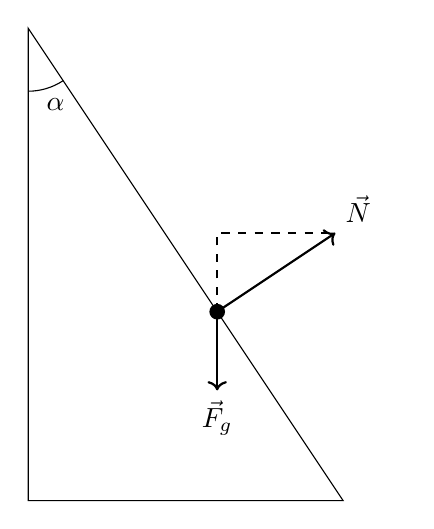
\begin{tikzpicture}
	    % Draw the triangle
	    \draw (0,0) -- (0,6) -- (4,0) -- cycle;

	    % Add the arc and label to the given angle
	    \draw (0,5.2) arc (-90:-56.31:0.8) coordinate (angle end);
	    \node [anchor=north west] at ($(0,5.2)!0.25!(angle end)$) {${\alpha}$};

	    % Pic an arbitrary point along the surface of the cone to represent
	    % the chain length element.
	    \coordinate (point) at ($(0,6)!0.6!(4,0)$);
	    \draw (point) node [fill,black,circle,inner sep=2pt] {};

	    % Draw the gravitational vector from the point
	    \draw [thick,->] (point) -- ++(0,-1)
		node [anchor=north] {$\vec F_g$};

	    % And the normal vector
	    \path [name path=Ny proj] ($(point)+(0,1)$) -- ($(point)+(2,1)$);
	    \path [name path=N vec] (point) -- ($(point)!1!90:(4,0)$);
	    \draw [name intersections={of=Ny proj and N vec, by=x}]
		[thick,->] (point) -- (x)
		node [anchor=south west] {$\vec N$}
		coordinate (norm end);

	    % Draw projections of the normal vector
	    \draw [thick,dashed] (point) -- ++(0,1) -- (norm end);
	\end{tikzpicture}
	\caption{Side View}
    \end{subfigure}
    \hfil
    \begin{subfigure}[b]{0.49\textwidth}
	\centering
	\begin{tikzpicture}
	    % Setup some coordinates:
	    \def\alpha{20}
	    \def\r{5cm}
	    \def\dr{0.2cm}
	    \def\Nr{1cm}
	    
	    \coordinate (center left)  at ($(90+\alpha:\r)$);
	    \coordinate (center mid)   at (90:\r);
	    \coordinate (center right) at ($(90-\alpha:\r)$);

	    \coordinate (outer left)   at ($(90+\alpha:\r+\dr)$);
	    \coordinate (outer mid)    at ($(90:\r+\dr)$);
	    \coordinate (outer right)  at ($(90-\alpha:\r+\dr)$);

	    \coordinate (inner left)   at ($(90+\alpha:\r-\dr)$);
	    \coordinate (inner mid)    at ($(90:\r-\dr)$);
	    \coordinate (inner right)  at ($(90-\alpha:\r-\dr)$);
	    
	    % Draw the radii
	    \draw [dashed] (0,0) -- (center left);
	    \draw [dashed] (0,0) -- (center mid);
	    \draw [dashed] (0,0) -- (center right);
	    % And label them
	    \node [anchor=west] at ($(0,0)!0.5!(center mid)$)   {$r$};
	    \node [anchor=west] at ($(0,0)!0.5!(center right)$) {$r$};

	    % Draw the chain
	    \draw [thick] (inner left) -- (outer left)
		arc (90+\alpha:90-\alpha:\r+\dr) -- (inner right)
		arc (90-\alpha:90+\alpha:\r-\dr);

	    % Draw the normal force
	    \draw (center mid) node [fill,black,circle,inner sep=2pt] {}
		node [anchor=west] {$ds$}
		[very thick,->] -- ++(0,\Nr)
		node [anchor=south] {$\vec N_r$};

	    % Finally, draw the tension vectors
	    \path [name path=Nr] ($(center mid)+(-4,-\Nr)$) -- ++(8,0);
	    \path [name path=Tl]
		(center left) -- ($(center left)!2.5cm!-90:(0,0)$);
	    \path [name path=Tr]
		(center right) -- ($(center right)!2.5cm!90:(0,0)$);

	    \draw [name intersections={of=Nr and Tl, by=x}]
		[very thick,->] (center left) -- (x)
		coordinate (left T end)
		node [anchor=north east] {$\vec T$};
	    \draw [name intersections={of=Nr and Tr, by=x}]
		[very thick,->] (center right) -- (x)
		coordinate (right T end)
		node [anchor=north west] {$\vec T$};
	    \draw [dashed] (left T end) -- (right T end);

	    % Add the known angles
	    \draw ($(0,0)!1cm!(center left)$) arc (90+\alpha:90-\alpha:1cm);
	    \node [anchor=south] at (0,1) {$d\phi $};
	    \draw ($(left T end)!1cm!(center left)$) arc ({\alpha}:0:1cm)
		node [anchor=north] {$\frac 12 d\phi $};
	\end{tikzpicture}
	\caption{Top View}
    \end{subfigure}
\end{figure}

Consider just a small element of the chain of arc length $ds$. It will have
a corresponding mass $dm = {\lambda}\,ds$ where ${\lambda} = m/L$. Knowing that it's a statics
problem, we can easily determine the normal force by balancing the vertical
component with that of gravity.
\begin{align*}
    F_g &= N \sin {\alpha} \\
    N &= \frac{{\lambda} g\,ds}{\sin {\alpha}}
\end{align*}
This leaves the horizontal component of the normal force to be balanced with
the tension within the chain.

Now switching to the top view, we consider the short chain segment $ds$, shown
above with an exagerated curvature. We note that the radial part of the
normal force must be opposed by the sum of the radial components of the two
tensions $T$ acting on the end of the chain segment. By geometry, we know that
the angle with respect to the midpoint's tangent is one half the differential
angle change $d\phi  = ds/r$. This means we balance the forces as
\begin{align*}
    2T\sin(\frac 12 d\phi ) &= N \cos {\alpha} \\
    2T\sin(\frac 12 d\phi ) &= {\lambda} g\,ds \cot {\alpha}
\end{align*}
By the small angle approximation, $\sin (\frac 12 d\phi ) \approx \frac 12 d\phi $, so after
substituting for the fact that $dr = L/2{\pi} $ and ${\lambda} = M/L$,
\begin{align}
    \boxed{
    T = \frac{Mg}{2{\pi} } \cot {\alpha}
    }
\end{align}

%%%%%%%%%%%%%%%%%%%%%%%%%%%%%%%%%%%%%%%%%%%%%%%%%%%%%%%%%%%%%%%%%%%%%%%%%%%%%%%
%%%% Problem 7
%%%%%%%%%%%%%%%%%%%%%%%%%%%%%%%%%%%%%%%%%%%%%%%%%%%%%%%%%%%%%%%%%%%%%%%%%%%%%%%
\problem{7}
\subsubsection{Question}
% Keywords
	\index{mechanics!Relativistic collision of electron and photon}

A laser beam (photon energy \SI{1}{\eV}) collides head-on with a \SI{50}{\GeV}
ultra-relativistic electron beam. What is the energy of the photons reflected
backwards in the collision?

\subsubsection{Answer}

We'll be solving the problem using conservation of 4-momentum, so we define
the following momenta with the assumption that the electron beam is moving
to the right, and the photons are initially moving to the left. Let the
unprimed and primed $q^{\mu}$ be the photon's 4-momentum before and after the
collision respectively, and define the electron's momenta $k^{\mu}$ similarly.
Then in terms of the energies $E$ and 3-momenta $p$ (actually taken to be 1D
without loss of generality) for each of the photon $\gamma $ and electron $e$:
\begin{align*}
    q^{\mu} &= \begin{pmatrix} E_\gamma /c \\ -E_\gamma /c \end{pmatrix} &
	q'^{\mu} &= \begin{pmatrix} E'_\gamma /c \\ E'_\gamma /c \end{pmatrix}
    \\
    k^{\mu} &= \begin{pmatrix} E_e/c \\ p_e \end{pmatrix} &
	k'^{\mu} &= \begin{pmatrix} E'_e/c \\ p'_e \end{pmatrix}    
\end{align*}
By conservation of momentum,
\begin{align*}
    q'^{\mu} + k'^{\mu} &= q^{\mu} + k^{\mu} \\
    k'^{\mu} &= q^{\mu} - q'^{\mu} + k^{\mu}
\end{align*}
Solving for the unknown electron momentum after the collision lets us eliminate
it from the equation; when we square the equation, the squared quantities are
Lorentz invariant, and therefore the product can be evaluated in any frame. A
convenient choice is the rest frame where the electron evaluates to its mass
energy and photons vanish.
\begin{align*}
    \underbrace{k'^{\mu} k'_{\mu}}_{m_e c^2} &=
	\underbrace{q^{\mu} q_{\mu}}_{0}
	- \underbrace{q'^{\mu} q'_{\mu}}_{0}
	+ \underbrace{k^{\mu} k_{\mu}}_{m_e c^2}
	- q'^{\mu} q_{\mu} + q'^{\mu} k_{\mu} - q^{\mu} k_{\mu}
\end{align*}
This greatly simplifies the rest of the problem to
\begin{align*}
    q'^{\mu} q_{\mu} - q'^{\mu} k_{\mu} &= - q^{\mu} k_{\mu}
\end{align*}
Inserting the energy and 3-momentum components and performing the inner
products,
\begin{align*}
    2\frac{E_\gamma  E'_\gamma }{c^2} - \frac{E'_\gamma  E_e}{c^2} + \frac{E'_\gamma  p_e}{c} &=
	-\frac{E_\gamma  E_e}{c^2} - \frac{E_\gamma  p_e}{c}
\end{align*}
Isolating $E'_\gamma $ on the left and $E_\gamma $ on the right,
\begin{align*}
    -E'_\gamma  (E_e - p_e c - 2E_\gamma ) &= - E_\gamma (E_e - p_e c)
\end{align*}
which solving for the unknown photon energy gives
\begin{align}
    \boxed{ E'_\gamma  = E_\gamma  (1 - \frac{2E_\gamma }{E_e - p_e c})^{-1} }
	\label{eqn:2002sp1.7:analytic_soln}
\end{align}

The solution is formally complete, but actually calculating a numerical answer
can prove difficult because $E_e \approx p_e c$. Therefore, we will expand the
solution. Beginning with the definition of the momentum from Einstein's energy
relation,
\begin{align*}
    p_e c &= \sqrt{{E_e}^2 - {m_e}^2c^4}
\intertext{we can subtract it from $E_e$, leading to the useful form}
    E_e - p_e c &= E_e ( 1 - \sqrt{1 - \frac{{m_e}^2c^4}{{E_e}^2}} )
\intertext{Expanding the root to first order in its argument,}
    E_e - p_e c &= E_e \cdot  \frac 12 \frac{{m_e}^2c^4}{{E_e}^2} \\
    {} &= \frac 12 \frac{{m_e}^2c^4}{E_e}
\end{align*}

Plugging this into the solution (\ref{eqn:2002sp1.7:analytic_soln}), the
photon energy is then approximately given by
\begin{align}
    \boxed{ E'_\gamma  \approx E_\gamma  ( 1 - 4 \frac{E_\gamma  E_e}{{m_e}^2c^4} )^{-1} }
	\label{eqn:2002sp1.7:approx_soln}
\end{align}
The numerics are much easier to calculate in this case, and we find that the
final energy of the reflected photon is
\begin{align}
    \boxed{ E'_\gamma  = \SI{4.273}{\eV} }
\end{align}

%%%%%%%%%%%%%%%%%%%%%%%%%%%%%%%%%%%%%%%%%%%%%%%%%%%%%%%%%%%%%%%%%%%%%%%%%%%%%%%
%%%% Problem 8
%%%%%%%%%%%%%%%%%%%%%%%%%%%%%%%%%%%%%%%%%%%%%%%%%%%%%%%%%%%%%%%%%%%%%%%%%%%%%%%
\problem{8}
\subsubsection{Question}
% Keywords
	\index{electrodynamics!LR circuit}

In the figure below, $\mathcal E = \SI{100}{\V}$, $R_1 = \SI{5}{\ohm}$,
$R_2 = \SI{10}{\ohm}$, $R_3 = \SI{15}{\ohm}$, and $L = \SI{1.0}{\henry}$. Find
the values of the currents $I_1$ and $I_2$
\begin{enumerate}[a)]
    \item immediately after the switch $S$ is closed,
    \item a long time later,
    \item immediately after switch $S$ is opened again,
    \item and then how long must you wait, after the switch is opened, before
	$I_2$ falls by a factor of $e$?
\end{enumerate}

\begin{center}
    \vspace{\baselineskip}
    \begin{circuitikz}
	\draw
	    (0,0)
		to[battery,l_=$\mathcal E$]
	    ++(0,3)
		to[closing switch,l_=$S$]
	    ++(3,0)
		to[resistor,l_=$R_1$]
	    ++(3,0)
		coordinate (I2 I3 break)
		to[resistor,l_=$R_3$,i=$I_3$]
	    ++(3,0)
		to[inductor,l_=$L$]
	    ++(0,-3)
		--
	    ++(-3,0)
		coordinate (I2 I3 combine)
		to[short,i=$I_1$]
	    (0,0)
	;
	\draw
	    (I2 I3 break)
		to[resistor,l_=$R_2$,i=$I_2$]
	    (I2 I3 combine)
	;
    \end{circuitikz}
    \vspace{\baselineskip}
\end{center}

\subsubsection{Answer}

Start by applying Kirchoff's rules to the circuit: current is conserved and
the voltage changes must sum to zero around each loop, so
\begin{align}
    I_1 &= I_2 + I_3
	\label{eqn:sp2002p1.8:kirchoff_current} \\
    0 &= \mathcal E - I_1R_1 - I_2R_2
	\label{eqn:sp2002p1.8:kirchoff_leftloop} \\
    0 &= -I_3R_3 - L \frac{dI_3}{dt} + I_2R_2
	\label{eqn:sp2002p1.8:kirchoff_rightloop}
\end{align}

Since only (\ref{eqn:sp2002p1.8:kirchoff_rightloop}) has a term involving
a time derivative, we choose to first solve for the current $I_3$. By solving
for $I_2R_2$ in (\ref{eqn:sp2002p1.8:kirchoff_leftloop}) and substituting,
we eliminate $I_2$ and have
\begin{align}
    0 &= -I_3R_3 - L\frac{dI_3}{dt} + \mathcal E - I_1R_1
    \label{eqn:sp2002p1.8:right_noI2}
\end{align}
Furthermore, by also substituting the value of $I_2$ into
(\ref{eqn:sp2002p1.8:kirchoff_current}):
\begin{align}
    I_1 &= \frac{\mathcal E}{R_1+R_2} + \frac{R_2}{R_1+R_2} I_3
    \label{eqn:sp2002p1.8:current_noI2}
\end{align}
Then by combining (\ref{eqn:sp2002p1.8:right_noI2}) and
(\ref{eqn:sp2002p1.8:current_noI2}), we can produce a differential equation
for $I_3$:
\begin{align*}
    -I_3R_3 - L\frac{dI_3}{dt} + \mathcal E - \frac{R_1}{R_1+R_2}\mathcal E -
	\frac{R_1R_2}{R_1+R_2}I_3 = 0
    \\
    -\underbrace{\frac{R_1R_2 + R_1R_3 + R_2R_3}{R_1+R_2}}_{R'}I_3 = L\frac{dI_3}{dt}
	- \frac{R_2}{R_1+R_2} \mathcal E
\end{align*}
\begin{align}
    \frac{dI_3}{dt} = -\frac{R'}{L} I_3 + \frac{1}{L}\frac{R_2}{R_1+R_2}\mathcal E
	\label{eqn:sp2002p1.8:diffeq_I3}
\end{align}
Considering just the homogeneous part, we easily solve it to find the standard
exponential solution
\begin{align*}
    I_{3h}(t) &= I_{30} e^{-R't/L}
\end{align*}
And using the ansatz $I_{3p}(t) = At + B$ for the inhomogeneous part,
\begin{align*}
    A &= -\frac{R'}{L}At - \frac{R'}{L}B + \frac 1L\frac{R_2}{R_1+R_2}\mathcal E
    \\
    A &= 0 \\
    B &= \frac{1}{R'}\frac{R_2}{R_1+R_2}\mathcal E
\end{align*}
At $t = 0$, the inductor has no current passing through it, so when the switch
is closed, the current must remain continuous. This gives us the initial
condition necessary to solve for the unknown $I_{30}$, and after doing so
and simplifying, the total solution is
\begin{align}
    I_3(t) &= \frac{\mathcal E}{R'}\frac{R_2}{R_1+R_2}(1 - e^{-R't/L})
	\label{eqn:sp2002p1.8:I3_charging}
\end{align}

Then by substituting this solution back into (\ref{eqn:sp2002p1.8:current_noI2})
we get the solution for $I_1$:
\begin{align}
    I_1(t) &= \frac{\mathcal E}{R_1+R_2} \left[ 1 + \frac{1}{R'}
	\frac{{R_2}^2}{R_1+R_2} (1 - e^{-R't/L}) \right]
	\label{eqn:sp2002p1.8:I1_charging}
\end{align}
Finally, combining both inserting both solutions for $I_1$ and $I_3$ into
(\ref{eqn:sp2002p1.8:kirchoff_current}), the solution for $I_2$ is
\begin{align}
    I_2(t) &= \frac{\mathcal E}{R_1+R_2} \left[ 1 - \frac{1}{R'}
	\frac{R_1R_2}{R_1+R_2} (1 - e^{-R't/L}) \right]
	\label{eqn:sp2002p1.8:I2_charging}
\end{align}

Plugging in all of the given values, we find that the currents at the instant
the switch is closed are
\begin{align}
    \boxed{I_1(0) = \SI{6.66}{\A}\quad\quad\text{$S$ is closed}} \\
    \boxed{I_2(0) = \SI{6.66}{\A}\quad\quad\text{$S$ is closed}}
\end{align}
For a long time later, we can let $t \rightarrow \infty $ and find that
\begin{align}
    \boxed{I_1(\infty ) = \SI{9.09}{\A}\quad\quad\text{$S$ is closed}} \\
    \boxed{I_2(\infty ) = \SI{5.54}{\A}\quad\quad\text{$S$ is closed}}
\end{align}

Right after the switch is opened, the left loop is taken out of the circuit,
so we immediately know that the value of $I_1$ is zero.
\begin{align}
    \boxed{I_1(0) = 0\quad\quad\text{$S$ is open	}}
\end{align}
For the right loop, we start by noting that the steady state current through
the inductor will be needed. Taking the limit of (\ref
{eqn:sp2002p1.8:I3_charging}), we have that the new initial condition is
\begin{align*}
    I_3(0) &= \frac{\mathcal E}{R'}\frac{R_2}{R_1+R_2}
\end{align*}
$I_2$ now is equal to $-I_3$ since there is no other path for the current to
traverse. This loop's differential equation is then
\begin{align*}
    -(R_2+R_3)I_3 - L\frac{dI_3}{dt} = 0
\end{align*}
Solving for the exponential and using the initial condition above, the time
solution is
\begin{align*}
    I_3(t) &= \frac{\mathcal E}{R'}\frac{R_2}{R_1+R_2} e^{-(R_2+R_3)t/L} \\
    I_2(t) &= -\frac{\mathcal E}{R'}\frac{R_2}{R_1+R_2} e^{-(R_2+R_3)t/L}    
\end{align*}
Therefore the current in $I_2$ just after the switch is opened reverses
direction
\begin{align}
    \boxed{I_2(0) = \SI{-3.64}{\A}}
\end{align}
Then by simple exponential relations, we know that the time time to decay by
a factor of $e$ is given by the reciprocal of the coefficient of $t$, so
inserting the appropriate numbers
\begin{align}
    \boxed{t_\mathrm{decay} = \SI{0.04}{\s}}
\end{align}

%%%%%%%%%%%%%%%%%%%%%%%%%%%%%%%%%%%%%%%%%%%%%%%%%%%%%%%%%%%%%%%%%%%%%%%%%%%%%%%
%%%% Problem 9
%%%%%%%%%%%%%%%%%%%%%%%%%%%%%%%%%%%%%%%%%%%%%%%%%%%%%%%%%%%%%%%%%%%%%%%%%%%%%%%
\problem{9}
\subsubsection{Question}
% Keywords
	\index{thermodynamics!Arbitrary engine efficiency}

An engine using \SI{1}{\mol} of an ideal diatomic gas performs the cycle $A
\rightarrow B \rightarrow C \rightarrow A$ as shown in the diagram below. $A
\rightarrow B$ is an adiabatic expansion, $B \rightarrow C$ occurs at
constant pressure, and $C \rightarrow A$ takes place at constant volume.
What is the efficiency of the cycle?

\begin{center}
    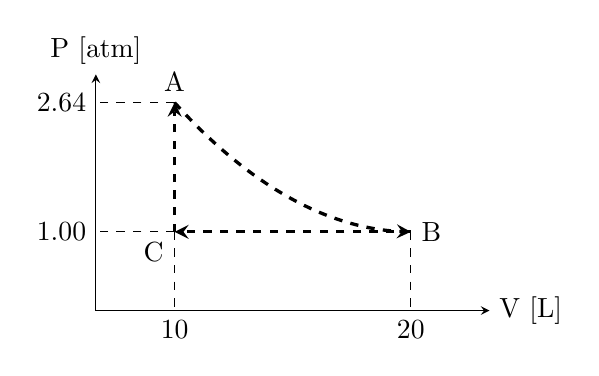
\begin{tikzpicture}[
	>=stealth
    ]
    % Draw the axes
	\draw [->] (0,0) -- (0,3) node [anchor=south] { P [\si{atm}] };
	\draw [->] (0,0) -- (5,0) node [anchor=west] {V [\si{\L}]};

	% Then draw the engine cycle
	\draw [very thick,dashed,->] (1,1)    -- (1, 2.64)
	    node [anchor=south] {A};
	\draw [very thick,dashed,->] (1,2.64) parabola[bend at end] (4,1)
	    node [anchor=west] {B};
	\draw [very thick,dashed,->] (4,1)    -- (1,1)
	    node [anchor=north east] {C};
	;

	% Then draw in the labels that give the absolute numbers
	\draw [dashed] (1,2.64) -- (0,2.64) node [anchor=east] {2.64};
	\draw [dashed] (1,1) -- (0,1) node [anchor=east] {1.00};
	\draw [dashed] (1,1) -- (1,0) node [anchor=north] {10};
	\draw [dashed] (4,1) -- (4,0) node [anchor=north] {20};
    \end{tikzpicture}
\end{center}

\subsubsection{Answer}

Since we want to find the efficiency of the cycle, we only care about the
heat exchanged during each stage of the cycle. Because the path $A
\rightarrow B$ is adiabatic, we immediately know that $Q = 0$. Then
proceeding to look at the stage $C \rightarrow A$, we know that the work
done during this cycle is identically zero since there is no area under the
curve. That means we are left simply with the equation
\begin{align*}
    dU = dQ
\end{align*}
Because this is an ideal [diatomic] classical gas, we combine the equations
\begin{align*}
    U &= \frac 52 nRT
\intertext{and}
    PV &= nRT
\end{align*}
to get that the difference in energy across the path is
\begin{align*}
    Q_{CA} &= U = \frac 52 nR(T_A - T_C) \\
    {}&= \frac 52 V_1 (P_2 - P_1)
\end{align*}

For the remaining stage $B \rightarrow C$, we use the full thermodynamic
identity:
\begin{align*}
    dU &= dQ - P\,dV
\end{align*}
The pressure $P_1$ is constant, so both integration of $dU$ and $dV$ are simply
the differences in each quantity. Again substituting for the temperature in
$U$ with the ideal gas law,
\begin{align*}
    \frac 52 nR(T_C - T_B) &= Q_{BC} - P_1(V_1 - V_2) \\
    \frac 52 P_1(V_1 - 2V_1) &= Q_{BC} + P(V_1 - 2V_1) \\
    Q_{BC} &= -\frac 72 P_1V_1
\end{align*}

We've accounted for all the heat flow in the system. $Q_{BC}$ is negative, so
this is the heat flow out of the system, while $Q_{CA}$ is positive and is the
heat flow into the system. By definition then, the efficiency ${\eta}$ of the system
is
\begin{align*}
    {\eta} &= 1 - \frac{Q_{out}}{Q_{in}} \\
    {}&= 1 - \frac{\frac 72 P_1 V_1}{\frac 52 V_1 (P_2 - P_1)} \\
    {}&= 1 - \frac 57 \frac{P_1}{P_2 - P_1}
\end{align*}
Plugging in the given values, we find the efficiency to be
\begin{align}
    \boxed{
    {\eta} = 0.146 = \SI{14.6}{\percent}
    }
\end{align}

%%%%%%%%%%%%%%%%%%%%%%%%%%%%%%%%%%%%%%%%%%%%%%%%%%%%%%%%%%%%%%%%%%%%%%%%%%%%%%%
%%%% Problem 10
%%%%%%%%%%%%%%%%%%%%%%%%%%%%%%%%%%%%%%%%%%%%%%%%%%%%%%%%%%%%%%%%%%%%%%%%%%%%%%%
\problem{10}
\subsubsection{Question}
% Keywords
	\index{mechanics!Friction and a rolling hoop}

A thin circular hoop rolls down an inclined plane under the influence of
gravity. What minimum coefficient of friction is required to ensure that it
rolls rather than slides?

\subsubsection{Answer}

Begin first by finding the motion that describes the rolling without slipping
state. We do this by solving the system's Lagrangian:
\begin{align*}
    \mathcal L &= (\frac 12 m{\dot x}^2 + \frac 12 I{\dot \theta }^2) - (mgx\sin {\alpha})
\end{align*}
where $x$ is the length along the ramp with $x=0$ at the bottom, $I$ is the
moment of inertia of the hoop, $m$ is its mass, $\theta $ is the angle of rotation
of the hoop about its center, and ${\alpha}$ is the angle of the incline plane. By
noting that rolling without slipping requires that $r\dot \theta  = \dot x$, we
can reduce the problem to the single variable $x$. The result is the following
differential equation, where $I = mR^2$ has been substituted in:
\begin{align*}
    2m \ddot x &= -mg\sin {\alpha} \\
    \ddot x &= -\frac 12 g\sin {\alpha}
\end{align*}
Therefore we know the linear acceleration will be $a = -\frac 12 g\sin {\alpha}$ in
the non-slipping case.

To find what coefficient of friction produces this motion, we consider the
forces acting on the hoop with the coordinate system still oriented along and
perpendicular to the plane. In the perpendicular direction, the normal force
$N$ is canceled by the perpendicular component of gravity, so
\begin{align*}
    N &= mg\cos {\alpha}
\end{align*}
In the parallel direction, the frictional force and the parallel component of
gravity must sum to give the requisite force, namely $ma$.
\begin{align*}
    {\mu}N - mg\sin {\alpha} &= ma = -\frac 12 mg\sin {\alpha} \\
    {\mu}mg\cos {\alpha} &= \frac 12 mg\sin {\alpha} \\
    {\mu} &= \frac 12 \tan {\alpha}
\end{align*}

\fbox{
Therefore we find that the coefficient of friction must be equal to half of
the tangent of the inclined plane's angle.
}

%%%%%%%%%%%%%%%%%%%%%%%%%%%%%%%%%%%%%%%%%%%%%%%%%%%%%%%%%%%%%%%%%%%%%%%%%%%%%%%
%%%% Problem 11
%%%%%%%%%%%%%%%%%%%%%%%%%%%%%%%%%%%%%%%%%%%%%%%%%%%%%%%%%%%%%%%%%%%%%%%%%%%%%%%
\problem{11}
\subsubsection{Question}
% Keywords
	\index{quantum!Probability to stay in ground state}

A particle is confined within a cubical box with sides of length $L$ and is
initially in the ground state. If the length of one side of the box (along
the $x$-direction) is abruptly increased to a length $2L$, what is the
probability that the particle remains in the ground state?

\subsubsection{Answer}

We start by recalling the solution for a particle in a box. In a 1D box with is
left edge at the origin, the properly normalized wavefunction is given by
\begin{align*}
    \psi (x) &= \sqrt{\frac{2}{L}} \sin (\frac{n{\pi} x}{L})
\end{align*}
where $L$ is the size of the box. The Cartesian extension into 3D is simple
and is respectively for the $L\times L\times L$ and $2L\times L\times L$ boxes:
\begin{align*}
    \psi (x,y,z) &= (\frac{2}{L})^{3/2} \sin(\frac{n_x {\pi} x}{L})
	\sin(\frac{n_y {\pi} y}{L}) \sin(\frac{n_y {\pi} y}{L}) \\
    \psi '(x,y,z) &= \frac{1}{\sqrt 2}(\frac{2}{L})^{3/2} \sin(\frac{n_x {\pi} x}{2L})
	\sin(\frac{n_y {\pi} y}{L}) \sin(\frac{n_y {\pi} y}{L})
\end{align*}

To find the probability of remaining in the ground state, we simply must
take the inner product of both wavefunctions in the ground state over an
appropriate domain; this means that the initial, unexanded box's wavefunction
is 0 within the new region.
\begin{align*}
    \mathscr{P} &= \braket{\psi _{111}}{\psi '_{111}} \\
    {} &= \frac{1}{\sqrt{2}} (\frac{2}{L})^3  (\int_0^L \sin(\frac{{\pi} x}{L})
	\sin(\frac{{\pi} x}{2L}) \,dx) (\int_0^L \sin(\frac{{\pi} y}{L})
	\sin(\frac{{\pi} y}{L}) \,dy) (\int_0^L \sin(\frac{{\pi} z}{L})
	\sin(\frac{{\pi} z}{L}))
\end{align*}
The integrals over $y$ and $z$ are simple and simply evaluate to $L/2$ as
we'd expect from the normalization factor. To evaluate the integral over $x$,
use the trigonometric identity $\sin 2\theta  = 2\sin \theta  \cos \theta $ and a change of
variables with $u = \sin({\pi} x/2L)$ to arrive at the integral
\begin{align*}
    \mathscr{P} &= \frac{2\sqrt 2}{L} \int_0^1 u^2 \cdot  \frac{2L}{{\pi} }\,du
\end{align*}
Evaluating this, we find the probability of remaining the ground state after
the box is expanded suddenly to be
\begin{align}
    \boxed{\mathscr{P} = \frac{4\sqrt 2}{3{\pi} } \approx 0.60}
\end{align}

%%%%%%%%%%%%%%%%%%%%%%%%%%%%%%%%%%%%%%%%%%%%%%%%%%%%%%%%%%%%%%%%%%%%%%%%%%%%%%%
%%%% Problem 12
%%%%%%%%%%%%%%%%%%%%%%%%%%%%%%%%%%%%%%%%%%%%%%%%%%%%%%%%%%%%%%%%%%%%%%%%%%%%%%%
\problem{12}
\subsubsection{Question}
% Keywords
	\index{mechanics!Deep-water gravity waves}
	\index{waves!Deep-water gravity waves}

The frequency $f$ of a deep water gravity wave (i.e. an ordinary ocean wave)
is given by
\begin{align*}
    f =\sqrt{\frac{1}{2{\pi} }} \rho ^a g^b {\lambda}^c
\end{align*}
where $\rho $, $g$, and ${\lambda}$ are the water density, gravitational acceleration, and
wavelength of the wave, respectively. What are the values of the exponents
$a$, $b$, and $c$, and what is the ratio of the wave group velocity to phase
velocity?

\subsubsection{Answer}

We proceed by dimensional analysis. Immediately we know that $a = 0$ since a
frequency does not have a mass component, and neither $g$ nor ${\lambda}$ have a
mass term to cancel the one in $\rho $. Furthermore, $g$ is the only one with a
time term, so it's exponent must then by $b = \frac 12$ in order to give $f$
its $[\si{\s^{-1}}]$ unit. That leaves $c = \frac 12$ in order to cancel
the $\sqrt{\si{\m}}$ dimension left over from $g$.

\begin{align*}
    \boxed{
    f = \sqrt{\frac{g{\lambda}}{2{\pi} }}
	\quad\quad\text{ with }\quad a = 0,\, b = \frac 12,\, c = \frac 12
    }
\end{align*}

The phase velocity can be derived from the frequency given by noting that
$v_p = {\omega} /k$ together with $k^{-1} = 2{\pi} {\lambda}$ and ${\omega}  = 2{\pi} f$. Put together, this
gives
\begin{align*}
    v_p &= \frac{1}{k}\sqrt{\frac{g}{k}}
\end{align*}
The group velocity is given by $v_g = d{\omega} /dk$, so
\begin{align*}
    v_g &= -\frac{1}{2k}\sqrt{\frac{g}{k}}
\end{align*}
Taking only the absolute values and finding the ratio
\begin{align}
    \boxed{\frac{v_g}{v_p} = \frac 12}
\end{align}


\springexam{2002}{2}
%%%%%%%%%%%%%%%%%%%%%%%%%%%%%%%%%%%%%%%%%%%%%%%%%%%%%%%%%%%%%%%%%%%%%%%%%%%%%%%
%%%% Problem 2
%%%%%%%%%%%%%%%%%%%%%%%%%%%%%%%%%%%%%%%%%%%%%%%%%%%%%%%%%%%%%%%%%%%%%%%%%%%%%%%
\problem{2}
\subsubsection{Question}
% Keywords
	\index{thermodynamics!Zipper partition function}
    \index{statistical mechanics!Zipper partition function}

A zipper has $N$ links; each link has a closed state with zero energy and an
open state with energy $\varepsilon $. We require, however, that the zipper can only
unzip from the left end, and that the link number $s$ can only open if all
links to the left (i.e.\ $1, 2, \ldots s-1$) are already open.
\begin{enumerate}[a.]
    \item
        Find an explicit expression for the partition function by doing the
        appropriate summation.
    \item
        In the limit $\varepsilon \gg k_B T$ find the average number of open links. This
        model is a very simplified model of the unwinding of two-stranded
        DNA molecules.
\end{enumerate}

\subsubsection{Answer}

\begin{enumerate}[a.]
    \item
        Create the partition function by induction; start by assuming there is
        only a single link. Then the partition function is a simple two-state
        system:
        \begin{align*}
            Z_1 &= e^0 + e^{-\varepsilon /k_BT} = 1 + e^{-\varepsilon /k_BT}
        \end{align*}
        Adding a second link,
        \begin{align*}
            Z_2 &= \underbrace{e^{0+0}}_{\text{both closed}} +
                \underbrace{e^{(-\varepsilon +0)/k_BT}}_{\text{1 open, 1 closed}} +
                \underbrace{e^{(-\varepsilon -\varepsilon )/k_BT}}_{\text{both open}}
            \\
            {} &= 1 + e^{-\varepsilon /k_BT} + e^{-2\varepsilon /k_BT}
        \end{align*}
        Following, for three links:
        \begin{align*}
            Z_3 &= \underbrace{e^{0+0+0}}_{\text{all closed}} +
                \underbrace{e^{(-\varepsilon +0+0)/k_BT}}_{\text{1 open, 2 closed}} +
                \underbrace{e^{(-\varepsilon -\varepsilon +0)/k_BT}}_{\text{2 open, 1 closed}} +
                \underbrace{e^{(-\varepsilon -\varepsilon -\varepsilon )/k_BT}}_{\text{all open}}
            \\
            {} &= 1 + e^{-\varepsilon /k_BT} + e^{-2\varepsilon /k_BT} + e^{-3\varepsilon /k_BT}
        \end{align*}
        By induction, we see that the maximum coefficient in the series of
        exponential factors is just the number of links, so by induction we
        conclude that
        \begin{align*}
            Z &= \sum_{s=0}^{N} e^{-s\varepsilon /k_BT}
        \end{align*}
        Applying the results of a finite geometric series, the closed-form
        solution for the partition function of the links is
        \begin{align}
            \boxed{
            Z = \frac{1 - e^{-(N+1)\varepsilon /k_BT}}{1 - e^{-\varepsilon /k_BT}}
            }
        \end{align}
    \item
        To get the average number of open links, we use the standard
        procedure for finding expvalation values.
        \begin{align*}
            \expval{s} &= \frac{1}{Z} \sum_{s=0}^N s e^{-s\varepsilon /k_BT}
        \end{align*}
        By making use of differentiation under the summation trick, we can
        find the closed-form solution:
        \begin{align*}
            \expval{s} &= \frac{1}{Z} \sum_{s=0}^N
                \frac{d}{d(\frac{\varepsilon }{k_BT})} \Big[ -e^{-s\varepsilon /k_BT} \Big] \\
            {} &= -\frac{1}{Z} \frac{\partial }{\partial (\frac{\varepsilon }{k_BT})}
                \sum_{s=0}^N e^{-s\varepsilon /k_BT} \\
        \intertext{
        Noting that the summation is the same as above,
        }
            \expval{s} &= -\frac{1}{Z} \frac{\partial Z}{\partial (\frac{\varepsilon }{k_BT})}
        \end{align*}
        First considering just the derivative part:
        \begin{align*}
            \frac{\partial Z}{\partial (\frac{\varepsilon }{k_BT})} &=
                \frac{(N+1)e^{-(N+1)\varepsilon /k_BT}}{1 - e^{-\varepsilon /k_BT}} -
                \frac{1 - e^{-(N+1)\varepsilon /k_BT}}{(1 - e^{-\varepsilon /k_BT})^2} e^{-\varepsilon /k_BT}
        \intertext{
        which when combined with the factor $-1/Z$ simplifies to
        }
            -\frac{1}{Z} \frac{\partial Z}{\partial (\frac{\varepsilon }{k_BT})} &=
                -(N+1)\frac{e^{-(N+1)\varepsilon /k_BT}}{1 - e^{-(N+1)\varepsilon /k_BT}} +
                \frac{e^{-\varepsilon /k_BT}}{1 - e^{-\varepsilon /k_BT}} \\
            &= \frac{1}{e^{\varepsilon /k_BT} - 1} - \frac{N+1}{e^{(N+1)\varepsilon /k_BT} - 1}
        \end{align*}
        Therefore the analytic solution is
        \begin{align}
            \boxed{
            \expval{s} = \frac{1}{e^{\varepsilon /k_BT}-1} - \frac{N+1}{e^{(N+1)\varepsilon /k_BT}-1}
            }
        \end{align}
        In the limit that $\varepsilon \gg k_BT$, though, the exponentials in the denominator
        are very large in comparison to 1, so we ignore the unity factors
        and make the approximation that
        \begin{align*}
            \expval{s} &= e^{-\varepsilon /k_BT} - (N+1)e^{-(N+1)\varepsilon /k_BT}
        \intertext{
        Collecting like terms,
        }
            {} &= \left[1 - (N+1)e^{-N\varepsilon /k_BT} \right] e^{-\varepsilon /k_BT}
        \intertext{
            The second term in the brackets approximate zero, so
        }
            {} &= e^{-\varepsilon /k_BT}
        \end{align*}
        Therefore in the low temperature limit where the thermal energy is
        much less than the energy of the open state,
        \begin{align}
            \boxed{
            \expval{s} = e^{-\varepsilon /k_BT}
            }
        \end{align}
\end{enumerate}


\fallexam{2002}{1}
%%%%%%%%%%%%%%%%%%%%%%%%%%%%%%%%%%%%%%%%%%%%%%%%%%%%%%%%%%%%%%%%%%%%%%%%%%%%%%%
%%%% Problem 5
%%%%%%%%%%%%%%%%%%%%%%%%%%%%%%%%%%%%%%%%%%%%%%%%%%%%%%%%%%%%%%%%%%%%%%%%%%%%%%%
\problem{5}
\subsubsection{Question}
% Keywords
	\index{mechanics!Elastic collision on spring-connected blocks}
	\index{Lagrangian!Elastic collision on spring-connected blocks}

Blocks of mass $m$ and $2m$ are free to slide without friction on a
horizontal wire. They are connected by a massless spring of equilibrium
length $L$ and force constant $k$. A projectile of mass $m$ is fired with
velocity $v$ into the block with mass $m$ and sticks to it. If the blocks
are initially at rest, what is the maximum displacement between them in the
subsequent motion?

\subsubsection{Answer}

Take time $t=0$ to be the moment the projectile collides with the mass $m$,
and let the subsequent transfer of momentum be instantaneous. In this case,
the initial conditions of the problem are then:
\begin{align*}
    x₁(0) &= 0			& \dot x₁(0) &= u \\
    x₂(0) &= L			& \dot x₂(0) &= 0
\end{align*}
where $u$ is the initial velocity of the combined project-mass system. We get
$u$ from conservation of mometum:
\begin{align*}
    2mu &= mv + 0 \\
    u &= \frac 12 v
\end{align*}

Now solve the mechanics problem using the Lagrangian approach. Both masses have
kinetic energy, and the spring stores potential energy, so
\begin{align*}
    T &= m{\dot x₁}² + m{\dot x₂}² \\
    V &= \frac 12 m (x₂ - x₁)² \\
    L &= m ({\dot x₁}² + {\dot x₂}²) - \frac 12 k({x₁}² + {x₂}² + 2x₁x₂)
\end{align*}
Setting up the differential equation, we get
\begin{align*}
    \frac{∂L}{∂x₁} &= -kx₁ + kx₂	& \frac{d}{dt}
	\left[\frac{∂L}{∂\dot x₁}\right] &= 2m \ddot x₁ \\
    \frac{∂L}{∂x₂} &=  kx₁ - kx₂	& \frac{d}{dt}
	\left[\frac{∂L}{∂\dot x₁}\right] &= 2m \ddot x₂ \\
\end{align*}
Leading to the system of equations where $ω² = k/2m$,
\begin{align*}
    \begin{bmatrix} \ddot x₁ \\ \ddot x₂ \end{bmatrix} &=
	\begin{bmatrix} -ω² & ω² \\ ω² & -ω² \end{bmatrix}
	\begin{bmatrix} x₁ \\ x₂ \end{bmatrix}
\end{align*}
Solving the eigensystem, we find the eigenfrequencies to be $λ = \{0, -2ω²\}$.
Letting ${ω'}² = 2ω²$, the eigenfunction equations are then
\begin{align*}
    \ddot ψ₁ &= 0
	& \rightarrow&&
	ψ₁ &= A₁t + B₁ \\
    \ddot ψ₂ &= -2ω² ψ₂
	& \rightarrow&&
	ψ₂ &= A₂\cos(ω't) + B₂\sin(ω't)
\end{align*}
From the eigenvectors, we express the solutions of $x₁$ and $x₂$ in terms of
$ψ₁$ and $ψ₂$:
\begin{align*}
    \begin{bmatrix} x₁ \\ x₂ \end{bmatrix} &=
	\begin{bmatrix} 1 & 1 \\ 1 & -1 \end{bmatrix}
	\begin{bmatrix} ψ₁ \\ ψ₂ \end{bmatrix}
\end{align*}
\begin{align*}
    x₁ &= A₁t + B₁ + A₂\cos(ω't) + B₂\sin(ω't) \\
    x₂ &= A₁t + B₁ - A₂\cos(ω't) - B₂\sin(ω't)
\end{align*}
Applying the boundary conditions, we find that
\begin{align*}
    x₁(t) &= \frac 14 vt + \frac 12 L - \frac 12 L\cos(ω't) +
	\frac{v}{4ω'}\sin(ω't) \\
    x₂(t) &= \frac 14 vt + \frac 12 L + \frac 12 L\cos(ω't) -
	\frac{v}{4ω'}\sin(ω't)
\end{align*}
The distance $ℓ(t) = x₂(t) - x₁(t)$ between the two masses maximizes when
\begin{align*}
    \frac{dℓ}{dt} = 0 &= \frac{d}{dt} \left[ L\cos(ω't) -
	\frac{v}{2ω'}\sin(ω't) \right] \\
    t &= -\frac{1}{ω'} \arctan (\frac{v}{2Lω'})
\end{align*}
Plugging back into the function $ℓ(t)$,
\begin{align*}
    ℓ &= L\cos \left[ -\arctan (\frac{v}{2Lω'}) \right] - \frac{v}{2ω'}
	\sin \left[ -\arctan (\frac{v}{2Lω'}) \right] \\
    ℓ &= L \frac{2Lω'}{\sqrt{v² + 4L² {ω'}²}} + \frac{v}{2ω'}
	\frac{v}{\sqrt{v² + 4L² {ω'}²}} \\
    ℓ &= \frac{\sqrt{v² + 4L² {ω'}²}}{2ω'}
\end{align*}
Finally, substituting back in $ω' = \sqrt{2k/m}$ and simplifying, we get the
final solution that maximum distance between the two masses is
\begin{empheq}[box=\fbox]{align}
    ℓ &= \sqrt{L² + \frac{\frac 12 mv²}{8k}}
\end{empheq}
which agrees qualitatively with the fact that a larger spring constant should
stiffen the system and decrease the maximum displacement, while launching the
projectile with a greater velocity would increase it.

%%%%%%%%%%%%%%%%%%%%%%%%%%%%%%%%%%%%%%%%%%%%%%%%%%%%%%%%%%%%%%%%%%%%%%%%%%%%%%%
%%%% Problem 10
%%%%%%%%%%%%%%%%%%%%%%%%%%%%%%%%%%%%%%%%%%%%%%%%%%%%%%%%%%%%%%%%%%%%%%%%%%%%%%%
\problem{10}
\subsubsection{Question}
% Keywords
	\index{dimensional analysis!Freezing ice}
	\index{thermodynamics!Freezing ice}

Ice on a pond is \SI{10}{\cm} thick and the water temperature just below the
ice is \SI{0}{\celsius}. If the air temperature is \SI{-20}{\celsius}, by
how much will the ice thickness increase in 1 hour? Assuming that the air
temperature stays the same over a long period, how will the ice thickness
increase with time? Comment on any approximation that you make in your
calculation.

Density of ice ${}= \SI{0.9}{\g\per\cm\cubed}$

Thermal conductivity of ice ${}= \SI{0.0005}{\cal\per\cm\per\s\per\celsius}$

Latent heat of fusion of water ${}= \SI{80}{\cal\per\g}$

\subsubsection{Answer}

Since the thermal heat flow is a one dimensional problem, immediately
consider everything with respect to a small area element with its normal
perpendicular to the ice-water interface $dA$. Then we want to know how much
ice is generated on the surface of the ice. This small ice element's mass is
simply
\begin{align*}
    dm &= ρ\,dA\,dz
\end{align*}
where $dz$ is the thickness of the new ice layer. To generate this ice, the
latent heat of fusion must be conducted away, so the energy released is,
\begin{align*}
    dE_f &= L_f\,dm \\
    {} &= L_f ρ \,dA\,dz
\end{align*}

The energy flow is through the ice, and we expect this to increase with the
temperature differential across the ice sheet, suggesting that the thermal
conductivity $κ$ be multiplied by the temperature difference $ΔT$. Furthermore,
the ice will decrease the rate of heat flow as it becomes thicker, so the
quantity should also be divided by the thickness $z$. This gives
\begin{align*}
    \frac{κ ΔT}{z} &= \left[ \si{\cal\per\cm\squared\per\s}
	\right]
\end{align*}
This energy is flowing through a surface element $dA$, giving the power flow
due to heat as
\begin{align*}
    \frac{κΔT\,dA}{z} &= \left[ \si{\cal\per\s} \right]
\end{align*}

This power can be matched in units with the energy released from the ice
calculated above by taking the time derivative of $dE_f$, so equating the two
we have
\begin{align*}
    L_f ρ \,dA\frac{dz}{dt} &= \frac{κΔT\,dA}{z} \\
    ∫_{z₀}^{z₀+δz} z\,dz &= ∫_0^t \frac{κΔT}{L_f ρ}\,dt \\
    2z₀ δz + (δz)² &= \frac{κΔT}{L_f ρ}t
\end{align*}
Solving for the length the ice grows $δz$,
\begin{align*}
    δz &= \frac{-2z₀ ± \sqrt{4{z₀}² - 4(\frac{κΔT}{L_f ρ})t} }{2} \\
    δz &= z₀(1 ± \sqrt{1 - \frac{κΔT}{L_f ρ {z₀}²} t})
\end{align*}
The two roots give solutions $δz = \{ \SI{0.0501}{\cm}, \SI{19.950}{\cm} \}$.
Since the second root is unrealistic, we know that the solution must then be
\begin{empheq}[box=\fbox]{align}
    δz &= \SI{0.0501}{\cm} \quad\text{in an hour}
\end{empheq}

%%%%%%%%%%%%%%%%%%%%%%%%%%%%%%%%%%%%%%%%%%%%%%%%%%%%%%%%%%%%%%%%%%%%%%%%%%%%%%%
%%%% Problem 11
%%%%%%%%%%%%%%%%%%%%%%%%%%%%%%%%%%%%%%%%%%%%%%%%%%%%%%%%%%%%%%%%%%%%%%%%%%%%%%%
\problem{11}
\subsubsection{Question}
% Keywords
	\index{statistical mechanics!Carbon-14 dating}

Carbon-14 is produced by cosmic rays interacting with the nitrogen in the
Earth's atmosphere. It is eventaully incorporated into all living things,
and since it has a half-life of \SI{5730(40)}{\year}, it is useful for
dating archaeological specimens up to several tens of thousands of years
old. The radioactivity of a particular specimen of wood containing \SI{3}{\g}
of carbon was measured with a counter whose efficiency was
\SI{18}{\percent}; a count rate of \SI{12.8(1)}{\minute^{-1}} was measured.
It is known that in \SI{1}{\g} of living wood, there are
\SI{16.1}{\minute^{-1}} radioactive carbon-14 decays. What is the age of
this specimen, and its uncertainity? (Where errors are not quoted, they can
be assumed to be negligible).

\subsubsection{Answer}
The rate $N$ after a given time is given by the exponential decay formula
\begin{align*}
    N(t) &+= N₀ e^{-t/τ}
\end{align*}
Since we have the half-life $t_{1/2}$ instead of the decay constant $τ$, we
use the relation $t_{1/2} = τ\ln 2$ to simplify the expression instead to
\begin{align*}
    N(t) &= N₀ (\frac 12)^{t/t_{1/2}}
\end{align*}

The counter use has an efficiency of $ε = 0.18$, so the measured counting
rate $N_m$ must be corrected for that. Furthermore, the sample has a mass of
\SI{3}{\g} whereas we know the rate for a one gram sample, so we also
normalize the count rate by the mass of the sample. Plugging this all into
the exponential decay function above gives
\begin{align*}
    \frac{N_m}{3ε} &= N₀ (\frac 12)^{t/t_{1/2}}
\end{align*}
The only unknown left in the equation is the time, so solving for it,
\begin{align*}
    t &= t_{1/2} \log_{1/2} (\frac{N_m}{3εN₀}) \\
    t &= t_{1/2} \frac{\ln (\frac{N_m}{3εN₀})}{\ln 2} \\
    t &= \frac{t_{1/2}}{\ln 2} \ln (\frac{N_m}{3εN₀})
\end{align*}

To find the uncertainty, we note that only the quantities $N_m$ and $t_{1/2}$
have non-negligible uncertainties, so we propagate the errors only over
these two terms:
\begin{align*}
    {σ_t}² &= (-\frac{t_{1/2}}{N_m \ln 2})² {σ_{N_m}}² +
	(\frac{1}{\ln 2} \ln(\frac{3εN₀}{N_m}))² {σ_{t_{1/2}}}² \\
    σ_t &= \frac{t_{1/2}}{\ln 2} \sqrt{ (\frac{σ_{N_m}}{N_m})² +
	(\frac{σ_{t_{1/2}}}{t_{1/2}})² \left[ \ln(\frac{3εN₀}{N_m}) \right]²}
\end{align*}
Plugging in all the numbers, we get $t = \SI{4248.8435}{\year}$ and $σ_t =
\SI{161.717}{\year}$. The given uncertainties have a single significant digit,
so adding an extra significant figure to the uncertainity and matching decimal
places in the answer, we conclude that the sample has an age of
\begin{empheq}[box=\fbox]{align}
    t &= \SI{4250(160)}{\year}
\end{empheq}


\fallexam{2007}{1}
%%%%%%%%%%%%%%%%%%%%%%%%%%%%%%%%%%%%%%%%%%%%%%%%%%%%%%%%%%%%%%%%%%%%%%%%%%%%%%%
%%%% Problem 9
%%%%%%%%%%%%%%%%%%%%%%%%%%%%%%%%%%%%%%%%%%%%%%%%%%%%%%%%%%%%%%%%%%%%%%%%%%%%%%%
\problem{9}
\subsubsection{Question}
% Keywords
	\index{thermodynamics!Light bulb as blackbody radiator}
	\index{circuits!Light bulb as blackbody radiator}

An electric bulb is rated at \SI{100}{\W} when used with a DC voltage of \SI
{110}{\V}. What total power is dissipated if this voltage is applied to two
such bulbs connected in series? It can be assumed that each bulb dissipates
heat by radiation from its filament similar to a black body and that the
resistance of the filament is proportional to its absolute temperature.

\subsubsection{Answer}

Beginning from the known properties of a single bulb, we know that the
dissipated power in a single bulb $P_0$ is like a black body, so the power
must follow the Stefan-Boltzmann law:
\begin{align*}
	P_0 &= {\sigma}_B {T_0}^4
\end{align*}
where $T_0$ is operating equilibrium temperature. In addition, we are told
that the bulb is like a resistor with a resistance proportional to its
temperature:
\begin{align*}
	P_0 &= \frac{V^2}{R} = \frac{V_0^2}{C T_0}
\end{align*}
Combining the two equations gives the proportionality constant for a single
bulb in the circuit.
\begin{align*}
	C &= \frac{{V_0}^2}{{\sigma}_B {T_0}^5}
\end{align*}

When a second bulb is added to the circuit, the voltage across each bulb is
dropped and a corresponding change in the equilibrium temperature is
created. Since the bulbs are in series, the voltage $V = \frac 12 V_0$ across
each resistor sums in series. Repeating the same procedure as in the first
case,
\begin{align*}
	{\sigma}_B T^4 &= 2 \frac{V^2}{R} = 2 \frac{(\frac 12 V_0)^2}{C T} \\
	{\sigma}_B T^5 &= \frac 12 \frac{{V_0}^2}{C}
\end{align*}
and inserting the constant $C$,
\begin{align*}
	T^5 &= \frac 18 {T_0}^5 \\
	T &= \frac{1}{2^{1/5}} T_0
\end{align*}
Therefore from the Stefan-Boltmann law, the total power dissipated is
\begin{align*}
	P &= {\sigma}_B T^4 = \frac{1}{2^{4/5}} {\sigma}_B {T_0}^4
\end{align*}
\begin{align}
	\boxed{ P = \frac{\SI{100}{\W}}{2^{4/5}} = \SI{57.435}{\W} }
\end{align}



\fallexam{2008}{1}
%%%%%%%%%%%%%%%%%%%%%%%%%%%%%%%%%%%%%%%%%%%%%%%%%%%%%%%%%%%%%%%%%%%%%%%%%%%%%%%
%%%% Problem 2
%%%%%%%%%%%%%%%%%%%%%%%%%%%%%%%%%%%%%%%%%%%%%%%%%%%%%%%%%%%%%%%%%%%%%%%%%%%%%%%
\problem{2}
\subsubsection{Question}
% Keywords
	\index{mechanics!Impulse on a rod}

If an impulse is delivered to the end of a uniform rod of length $ℓ$, lying on
a frictionless plane, how far will it travel while making one revolution? The
impulse is in the plane of the table and perpendicular to the rod.

\subsubsection{Answer}

For a given impulse $\vec J$, the change in the motion is $\vec J = Δ\vec p$.
If the rod start at rest, then the final momentum must be $\vec p = \vec J$.
This means the rod is moving laterally with a velocity
\begin{align*}
    V = \frac 1m \vec J
\end{align*}
which when integrated over a time $t$ gives the distance it has moved $\vec x$.
\begin{align*}
    \vec x = \frac 1m \vec J t
\end{align*}

The impulse also imparts a rotation on the rod because the force was not
applied at the rod's center of mass. The torque $\vec τ$ relates the force
to the angular momentum $\vec L$ by
\begin{align*}
    \vec r × \vec F &= \vec τ = \dot{\vec L}
\end{align*}
Integrating both sides of the equation, we can write the equation in terms of
the given impulse:
\begin{align*}
    \vec r × \int \vec F \,dt &= \int \dot{\vec L} \,dt \\
    \vec r × \vec J &= Δ\vec L
\end{align*}
Again, since the rod starts at rest, we know that the final angular momentum
must be
\begin{align*}
    \vec L = \vec r × \vec J
\end{align*}
The rotation about the rod's center of mass  occurs at a rate $\vec ω$
dependent on the moment of inertia $I = \frac{1}{12} mℓ²$, so
\begin{align*}
    \vec ω = \frac{12}{mℓ²} \vec r × \vec J
\end{align*}
We know that the impulse is applied perpendicular to the rod, so we can easily
integrate the expression in time and solve for the time it takes to revolve
$2π$ radians:
\begin{align*}
    θ = 2π &= \frac{12}{mℓ²} rJt \\
    t &= \frac{πmℓ²}{6 rJ}
\end{align*}

Plugging this back into the linear motion equation, the rod travels
\begin{align*}
    \vec x = \frac{1}{m} \vec J ⋅ \frac{πmℓ²}{6 rJ}
\end{align*}
where we can set $r = \frac 12 ℓ$ and therefore simplifies to
\begin{align}
    \boxed{
    \vec x = \frac{πℓ}{3} \hat J
    }
\end{align}
where $\hat J$ is the direction of the applied impulse.

%%%%%%%%%%%%%%%%%%%%%%%%%%%%%%%%%%%%%%%%%%%%%%%%%%%%%%%%%%%%%%%%%%%%%%%%%%%%%%%
%%%% Problem 3
%%%%%%%%%%%%%%%%%%%%%%%%%%%%%%%%%%%%%%%%%%%%%%%%%%%%%%%%%%%%%%%%%%%%%%%%%%%%%%%
\problem{3}
\subsubsection{Question}
% Keywords
	\index{electrodynamics!Properties of a magnetic field}

A time-indpendent magnetic field is given by $\vec B = 2bxy \,\hat ı +
ay² \,\hat ȷ$.
\begin{enumerate}[a)]
    \item
        What is the relationship between the constants $a$ and $b$?
    \item
        Determine the steady current density $J$ that gives rise to this field.
\end{enumerate}

\subsubsection{Answer}
For part (a), we realize that all magnetic fields must be divergenceless.
Therefore we can find the requirements on the constants $a$ and $b$ by
constraining the divergence to be zero.
\begin{align*}
    \vec ∇ ⋅ \vec B = 0 &= \frac{∂}{∂x}(2bxy) + \frac{∂}{∂y}(ay²) \\
    0 &= 2by + 2ay \\
    b &= -a
\end{align*}
Therefore the relation between the constants is that
\begin{align}
    \boxed {b = -a}
\end{align}

For the second part, we make use of Maxwell's equations. Assuming that none of
the field is due to a time-varying electric field, we make use of
\begin{align*}
    \vec ∇ × \vec B &= μ₀ \vec J
\end{align*}
to calculate the current that generates the field. Doing so, we find that the
solution is
\begin{align}
    \boxed{ \vec J = \frac{2a}{μ₀} x \,\hat k }
\end{align}

%%%%%%%%%%%%%%%%%%%%%%%%%%%%%%%%%%%%%%%%%%%%%%%%%%%%%%%%%%%%%%%%%%%%%%%%%%%%%%%
%%%% Problem 4
%%%%%%%%%%%%%%%%%%%%%%%%%%%%%%%%%%%%%%%%%%%%%%%%%%%%%%%%%%%%%%%%%%%%%%%%%%%%%%%
\problem{4}
\subsubsection{Question}
% Keywords
	\index{electrodynamics!Charges from multipole moments}

A set of four point charges $q₁$, $q₂$, $q₃$, and $q₄$ are arranged
collinearly along the $z$-axis at $z₁ = 0$, $z₂ = a$, $z₃ = 2a$, $z₄ = 4a$,
respectively and the resulting electric field at a distant point $\vec r$ ($r
≫ a$) decays \emph{faster} than $1/r³$. Determine the values of $q₁$ and $q₄$
which $q₂ = +2$ and $q₃ = +4$. Units for all charges are Coulombs.

\subsubsection{Answer}

Given that the electric field must fall off faster than $1/r³$, this
corresponds to a potential which drops off faster than $1/r²$. We know that
the monopole moment drops off like $1/r$ and the dipole like $1/r²$, so we
conclude that the first configuration which could satisfy the given
requirement is that of a quadrupole moment.

Making use of the fact that he monopole and dipole moments are vanishing, we
can use them to generate constraint equations for what the charges must be:
we have two unknown charges and the two equations will allow us to solve them.

For the monopole, the sum of all charges must simply equal zero. Therefore
we immediately know that
\begin{align*}
    0 &= q₁ + q₄ + 6 \\
    -6 &= q₁ + q₄
\end{align*}

The dipole moment (where we take the dipole considered at the origin) is given
by
\begin{align*}
    \vec p = \sum_i \vec{r_i} q_i
\end{align*}
This gives us the equation
\begin{align*}
    0 &= 10a + 4aq₄ \\
    q₄ &= -\frac 52
\end{align*}
The charge $q₁$ does not show up in the equation since it is located at the
origin. This lets us very simply then solve for $q₁$ as
\begin{align*}
    -6 &= q₁ - \frac 52
\end{align*}
Therefore, the solution is that the charges have values of
\begin{align}
    \boxed{ q₁ = -\frac 72 } \\
    \boxed{ q₄ = -\frac 52 }
\end{align}

%%%%%%%%%%%%%%%%%%%%%%%%%%%%%%%%%%%%%%%%%%%%%%%%%%%%%%%%%%%%%%%%%%%%%%%%%%%%%%%
%%%% Problem 5
%%%%%%%%%%%%%%%%%%%%%%%%%%%%%%%%%%%%%%%%%%%%%%%%%%%%%%%%%%%%%%%%%%%%%%%%%%%%%%%
\problem{5}
\subsubsection{Question}
% Keywords
	\index{quantum!Spectral emission line width}

The Lyman-α transition in atomic hydrogen has a wavelength $λ =
\SI{121.5}{\nm}$, and a transition rate of \SI{0.6e9}{\s^{-1}}. Estimate the
minimum value of $Δλ/λ$.

\subsubsection{Answer}

We can make an estimate of the spread $Δλ$ by making use of the Heisenberg
uncertainty relation for energy-time. Starting with the variation in
wavelength,
\begin{align*}
    Δλ &= λ - λ' \\
    {} &= \frac{hc}{E} - \frac{hc}{E'} \\
    {} &= \frac{hc(E' - E)}{E E'}
\intertext{Making use of the approximation that $E ≈ E'$,}
    {} &= \frac{hcΔE}{E²}
\end{align*}
Dividing by the frequency and substituting in the uncertainty relation $ΔEΔt =
\frac{ℏ}{2}$,
\begin{align*}
    \frac{Δλ}{λ} &= \frac{hc}{λ} ⋅ \frac{1}{E²}\frac{ℏ}{2Δt} \\
    {} &= \frac{λ}{4πcΔt}
\end{align*}
For the time, we estimate the transition rate is occuring as fast as it can
within the limits of the uncertainty relation, so we can let $Δt ≈ \SI{0.6e9}
{\s^{-1}}$. Plugging in the other values, we find the fractional line width
to be estimated as
\begin{align}
    \boxed{ \frac{Δλ}{λ} ≈ \num{1.935e-8} ≈ \text{1 part in 50 million} }
\end{align}

%%%%%%%%%%%%%%%%%%%%%%%%%%%%%%%%%%%%%%%%%%%%%%%%%%%%%%%%%%%%%%%%%%%%%%%%%%%%%%%
%%%% Problem 11
%%%%%%%%%%%%%%%%%%%%%%%%%%%%%%%%%%%%%%%%%%%%%%%%%%%%%%%%%%%%%%%%%%%%%%%%%%%%%%%
\problem{11}
\subsubsection{Question}
% Keywords
	\index{statistical mechanics!Radiometric dating from mass ratios}

A rock is found to contain \SI{4.20}{\mg} of ${}^{238}U$ and \SI{2.00}{\mg}
of ${}^{206}Pb$. Assume tha the rock contained no lead at the time of its
formation, so that all the lead now present is due to th decay of the
uranium orignally present in the rock. Find the age of the rock given that
the half-life of ${}^{238}U$ is \SI{4.47e9}{\year}. The decay times of all
intermediate elements are negligibly short and ignore any differences in the
binding energies.

\subsubsection{Answer}

From decay processes, we know that the uranium atom count will decrease as an
exponential according to
\begin{align*}
    N_U = N_{U0}e^{-t/τ}
\end{align*}
where $τ = t_{1/2}/\ln 2$. Likewise, the number of lead atoms will increase
according to
\begin{align*}
    N_{Pb} = N_{U0} (1 - e^{-t/τ})
\end{align*}
Solveing for $N_{U0}$ in the first equation and substituting it into the
second, we can solve for the time required to generate a specific number of
uranium and lead atoms in a sample.
\begin{align*}
    N_{Pb} &= N_U e^{t/τ} (1 - e^{-t/τ}) \\
    t &= τ \ln(\frac{N_{Pb}}{N_U} + 1) \\
    t &= \frac{t_{1/2}}{\ln 2} \ln(\frac{N_{Pb}}{N_U} + 1)
\end{align*}
We were only given the masses, though, so we approximate the mass of each
atom by the number of nucleons in the nucleus; each uranium atom has a mass
of $m_U = 238m_N$ making the $N_U$ atoms have a mass of $M_U = 238 N_U m_N$,
and similar for the lead. This gives us the final equation
\begin{align*}
    t &= \frac{t_{1/2}}{\ln 2} \ln(\frac{238}{206} \frac{M_{Pb}}{M_U} + 1)
\end{align*}
Plugging in all the numbers,
\begin{align}
    \boxed{ t = \SI{2.83e9}{\year} }
\end{align}

%%%%%%%%%%%%%%%%%%%%%%%%%%%%%%%%%%%%%%%%%%%%%%%%%%%%%%%%%%%%%%%%%%%%%%%%%%%%%%%
%%%% Problem 12
%%%%%%%%%%%%%%%%%%%%%%%%%%%%%%%%%%%%%%%%%%%%%%%%%%%%%%%%%%%%%%%%%%%%%%%%%%%%%%%
\problem{12}
\subsubsection{Question}
% Keywords
	\index{circuits!Current amplitude and phase in LRC circuit}

The applied AC voltage in the circuit is given by $V(t) = V₀ \sin ωt$, with 
a frequency fixed at $ω = 1/(LC)^{1/2}$. Determine the steady state 
amplitude and phase of the current through the resistor $R$. Express your 
answer in terms of the amplitude $V₀$ of the applied voltage and the other 
circuit parameters.

\begin{center}
	\vspace{\baselineskip}
	\begin{circuitikz}
		\resetparens
		\draw (0,-2)
		to [sV,l=$V(t)$] ++(0,4)
			-- ++(3,0)
		to [L,l=$L$] ++(0,-2)
			coordinate (split)
			-- ++(-1,0)
		to [C,l=$C$] ++(0,-2)
			-- (0,-2)
			(split) -- ++(1,0)
		to [R,l=$R$] ++(0,-2)
			-- (0,-2)
		;
	\end{circuitikz}
	\vspace{\baselineskip}
\end{center}

\subsubsection{Answer}

AC problems are simplified by using complex impedances, so we first convert 
the given voltage into a complex one:
\begin{align*}
	\tilde V(t) &= V₀ e^{iωt}
\end{align*}
where the physical solution can be recovered by keeping the imaginary 
component of the complex solution. Then to solve the problem, we realize 
that there is another complimentary circuit diagram which is helpful: the 
one with the resistor and capacitor replaced by an effective resistor 
(impedance). The circuit looks like
\begin{center}
	\vspace{\baselineskip}
	\begin{circuitikz}
		\resetparens
		\draw (0,-2)
		to [sV,l=$V(t)$] ++(0,4)
			-- ++(3,0)
		to [R,l=$Z_L$] ++(0,-2)
		to [R,l=$Z_{eff}$] ++(0,-2)
			-- (0,-2)
		;
	\end{circuitikz}
	\vspace{\baselineskip}
\end{center}
The inductor has been been replaced by an effective resistor with impedance 
$Z_L = iωL$. The effective resistor that replaced the capacitor and resistor 
is a complex impedance that is calculated the same as for traditional 
resistors in parallel:
\begin{align*}
	Z_{eff} &= ( \frac{1}{Z_C} + \frac{1}{Z_R} )^{-1} \\
		&= ( iωC + \frac{1}{R} )^{-1} \\
		&= \frac{R}{iωCR + 1}
\end{align*}
Now making use of Kirchoff's loop rule on this simplified circuit where the 
total current passing through the voltage source is labeled $\tilde I₀$,
\begin{align*}
	0 &= \tilde V - \tilde I₀ (Z_L + Z_{eff}) \\
	\tilde V &= (iωL + \frac{R}{iωCR + 1}) \tilde I₀ \\
	\tilde V &= \frac{R(1 - ω²LC) + iωL}{iωRC + 1} \tilde I₀
\intertext{The first term in the numerator goes to zero since $ω² = 1/LC$,
leaving}
	\tilde I₀ &= \frac{iωRC + 1}{iωL} V₀ e^{iωt}
\end{align*}

To isolate the current passing through the resistor, we return to the 
original unsimplified circuit diagram and apply Kirchoff's loop rule to only 
the inner loop. If we define the current through capacitor to be $I₁$ and
through the resistor to be $I₂$, we get
\begin{align*}
	0 &= -\tilde I₂ Z_R + \tilde I₁ Z_C \\
	\tilde I₁ &= \frac{Z_R}{Z_C} I₂ \\
	\tilde I₁ &= iωRC I₂ \\	
\end{align*}
Remembering the the current passing into a junction must be conserved, we know
that $I₀ = I₁ + I₂$ and therefore,
\begin{align*}
	\tilde I₀ &= iωRC \tilde I₂ + \tilde I₂ \\
	\tilde I₂ &= \frac{1}{iωRC + 1} \tilde I₀
\end{align*}
Inserting the solution for $I₀$ from the previous part leaves
\begin{align*}
	\tilde I₂ &= \frac{V₀}{iωL} e^{iωt}
\end{align*}
To prepare for finding the physical solution, we transform the coefficient
complex polar form.
\begin{align*}
	\tilde I₂ &= \left|-\frac{iV₀}{ωL}\right| e^{i\arg(-iV₀/ωL)} e^{iωt} \\
		&= \frac{V₀}{ωL} e^{-iπ/2} e^{iωt}
\end{align*}
Therefore taking the imaginary part of the solution,
\begin{align}
	\boxed{
	I_R(t) = V₀ \sqrt{\frac{C}{L}} \sin(ωt - \frac π2)
	}
\end{align}
The current's amplitude is $V₀\sqrt{C/L}$ and has a phase of $-π/2$ with
respect to the voltage.


\fallexam{2008}{2}
%%%%%%%%%%%%%%%%%%%%%%%%%%%%%%%%%%%%%%%%%%%%%%%%%%%%%%%%%%%%%%%%%%%%%%%%%%%%%%%
%%%% Problem 1
%%%%%%%%%%%%%%%%%%%%%%%%%%%%%%%%%%%%%%%%%%%%%%%%%%%%%%%%%%%%%%%%%%%%%%%%%%%%%%%
\problem{1}
\subsubsection{Question}
% Keywords
	\index{Lagrangian!Bead on a Wire}
    \index{mechanics!Small Oscillations}

A particle of mass $m$ is constrained to move without friction on a circular
wire of radius $R$ rotating with constant angular frequency ${\omega}$ about a
vertical diameter. Gravity can not be neglected.
\begin{enumerate}[a)]
    \item
        Write down the Lagrangian for the system and the equations of motion.
    \item
        Find the equilibrium position(s) of the particle and determine
        whether this position is stable.
    \item
        Calculate the frequency of small oscillations about any stable points.
\end{enumerate}

\begin{figure}[H]
    \centering
    \begin{tikzpicture}
        % The axis
        \draw [dashed,->] (0,-1) -- (0,4);
        % The hoop
        \draw (0,1.5) circle (1.5);
        % The bead
        \draw ($(0,1.5)!1.5cm!30:(0,0)$)
            node[circle,fill=black,anchor=center,inner sep=2pt] {}
            coordinate (bead);
        % Label the angle
        \draw [dashed] (0,1.5) -- (bead);
        \draw ($(0,1.5)!0.5cm!(0,0)$)
            coordinate (arc start)
            arc (-90:-60:0.5cm)
            coordinate (arc end);
        \draw ($(arc start)!0.5!(arc end)$)
            node [anchor=north] {$\,\,\theta $};
    \end{tikzpicture}
\end{figure}

\subsubsection{Answer}

To start constructing the Lagrangian and equations of motion, we first specify
the kinetic and potential energies. For the kinetic energy, there is an energy
associated with the rotation about the axis and one along the bead. These
combined to give
\begin{align*}
    T &= \frac 12 m (R{\omega}\sin \theta )^2 + \frac 12 m (R\dot \theta )^2 \\
    {} &= \frac 12 m R^2 {\omega}^2 \sin^2 \theta  + \frac 12 m R^2 {\dot \theta }^2
\end{align*}
The potential energy is all gravitational, so
\begin{align*}
    V &= -mgR\cos \theta 
\end{align*}
where the zero point was taken to be at the center of the hoop to avoid adding
extra constant terms to the Lagrangian. Combining the two, we get
\begin{align}
    \boxed{
    \mathcal L = \frac 12 mR^2{\omega}^2\sin^2 \theta  + \frac 12 mR^2{\dot \theta }^2 + mgR\cos \theta 
    }
\end{align}
Taking the appropriate derivatives in $\theta $, the equation of motion is
\begin{align}
    \boxed{
    \ddot \theta  = {\omega}^2 \sin \theta  \cos \theta  - \frac{g}{R}\sin \theta 
    }
\end{align}

In order to determine any possible stable points, we note that a stable point
is a place where the angle does not change in time. Since this also equates to
$\ddot \theta  = 0$, we set the equation above equal to zero and solve for the angles
which satisfy this condition. They end up being the trivial $\theta  = \{0, {\pi}\}$
where the sine function is zero as well as
\begin{align*}
    \cos \theta _0 &= \frac{g}{R{\omega}^2}
\end{align*}
The three stable points are then
\begin{align}
    \boxed{ \theta _0 = \left\{ 0, \arccos(\frac{g}{R{\omega}^2}), {\pi} \right\} }
\end{align}

To determine the stability of each, we must determine whether we get
oscillatory or exponential solutions to the differential equation of motion.
To do this, we suppose the angle $\theta $ is composed of the equilibrium angle
$\theta _0$ and a small perturbation $\Delta $. Expanding the equation in terms of this,
\begin{align*}
    \ddot \Delta  = {\omega}^2\sin(\theta _0+\Delta )\cos(\theta _0+\Delta ) - \frac{g}{R}\sin(\theta _0+\Delta )
\end{align*}
Using several trigonometric expansions, the equation can be expanded into the
form
\begin{align*}
    \ddot \Delta  = {\omega}^2\left[ \cos \theta _0\sin \theta _0 (\cos^2\Delta  - \sin^2\Delta ) + \cos \Delta \sin \Delta 
        (\cos^2\theta _0 - \sin^2\theta _0) \right] - \frac{g}{R}\left[ \sin \theta _0\cos \Delta  +
        \cos \theta _0\sin \Delta  \right]   
\end{align*}

For the case where $\theta _0 = 0$,
\begin{align*}
    \ddot \Delta  &= {\omega}^2 \cos \Delta  \sin \Delta  - \frac{g}{R} \sin \Delta 
\intertext{Expanding to first order in $\Delta  \approx 0$,}
    \ddot \Delta  &= -(\frac{g}{R} - {\omega}^2)\Delta 
\end{align*}
Therefore, the equilibrium point $\theta _0 = 0$ is only stable if ${\omega} <
\sqrt{\frac{g}{R}}$.

Likewise for for $\theta _0 = {\pi}$,
\begin{align*}
    \ddot \Delta  &= (\frac{g}{R} + {\omega}^2) \Delta 
\end{align*}
The coefficient on $\Delta $ will never be negative, so the angle $\theta _0 = {\pi}$ will
be unstable under all conditions.

For the final angle where $\theta _0 = \arccos(\frac{g}{R{\omega}^2})$, we must do several
substitutions and expansions. $\cos \theta _0$ is trivial. $\sin \theta _0$ ends up being
$\sqrt{R{\omega}^2 - g^2}/(R{\omega}^2)$ by triangle relations. If we substitute these in plus
do an expansion to first order for small $\Delta $, we get the equation
\begin{align*}
    \ddot \Delta  &= {\omega}^2 \left[ \frac{g\sqrt{R{\omega}^2-g^2}}{R^2{\omega}^2} + \Delta  \frac{2g^2-R{\omega}^2}{R^2{\omega}^2}
        \right] - \frac{g}{R} \left[\frac{\sqrt{R{\omega}^2-g^2}}{R^2{\omega}^2} + \Delta 
        \frac{g}{R{\omega}^2} \right]
\end{align*}
If we consider only the homogeneous terms dependent on $\Delta $,
\begin{align*}
    \ddot \Delta  &= \frac{g^2 - R{\omega}^2}{R^2{\omega}^2} \Delta 
\end{align*}
This equation is stable if and only if the coefficient on $\Delta $ is negative, so
it must be that ${\omega} > \frac{g}{\sqrt{R}}$.

In summary, the equilibrium points have the following conditions:
\begin{align}
    \boxed{ \theta _0 = 0 \quad\quad \text{Stable iff } {\omega} < \sqrt{\frac gR} }
\end{align}
\begin{align}
    \boxed{ \theta _0 = \arccos(\frac{g}{R{\omega}^2}) \quad\quad \text{Stable iff }
        {\omega} > \frac{g}{\sqrt{R}} }
\end{align}
\begin{align}
    \boxed{ \theta _0 = {\pi}  \quad\quad \text{Never stable} }
\end{align}


About the two stable points, we simply use the coefficient that has already
been isolated to determine the frequency of the oscillations about that point.
\begin{align}
    \boxed{ {\omega}_1 = \sqrt{\frac{g}{R} - {\omega}^2} \quad\quad\text{for $\theta _0 = 0$} }
\end{align}
\begin{align}
    \boxed{ {\omega}_2 = \sqrt{\frac{R{\omega}^2 - g^2}{R^2{\omega}^2}}\quad\quad\text{for $\theta _0 =
        \arccos(\frac{g}{R{\omega}^2})$} }
\end{align}

%%%%%%%%%%%%%%%%%%%%%%%%%%%%%%%%%%%%%%%%%%%%%%%%%%%%%%%%%%%%%%%%%%%%%%%%%%%%%%%
%%%% Problem 2
%%%%%%%%%%%%%%%%%%%%%%%%%%%%%%%%%%%%%%%%%%%%%%%%%%%%%%%%%%%%%%%%%%%%%%%%%%%%%%%
\problem{2}
\subsubsection{Question}
% Keywords
	\index{electrostatics!Charged sphere in uniform electric field}
    \index{Gauss' Law!Charged sphere in uniform electric field}

The general solution of the Laplace's equation for an electrostatic problem
having azimuthal symmetry can be written as
\begin{align*}
    V(r,\theta ) &= \sum_{\ell =0}^\infty  (A_\ell  r^\ell  + \frac{B_\ell }{r^{\ell +1}}) P_\ell (\cos \theta )
\end{align*}
Now consider the following problem. A solid spherical conductor of radius $R$
having charge $Q$ is placed in an otherwise uniform electric field $\vec E
= E_0\hat z$.
\begin{enumerate}[(a)]
    \item
        Qualitatively describe the electric field inside and outside of the
        sphere.
    \item
        Solve the problem and find the electric potential in the region outside
        the sphere.
\end{enumerate}

\subsubsection{Answer}

To provide a qualitative description, we make use of several properties of
conductors. The electric field inside the conductor is guaranteed to be zero
in the limit of a perfect conductor which can move its electrons anywhere
they're needed to cancel any applied fields. For the region outside the
sphere, it is easiest to describe the region just outside the surface and
the region at infinitely large distances. Far away, the effects of the the
sphere are negligible and the electric field is the external uniform field.
Near the surface, though, all field lines are perpendicular to the surface;
therefore, the external field's lines are curved so that any intersections
occur perpendicular to the surface.

In summary
\par\fbox{\begin{minipage}{\textwidth}
    \begin{enumerate}
        \item
            The field is uniform at large distances
        \item
            The field is perpendicular to the surface of the conductor at
            the conductor's surface
        \item
            There is no field within the interior of the conductor
    \end{enumerate}
\end{minipage}}
\vspace{\baselineskip}

In order to analyze the problem analytically, we make use of the
superposition principle to simplify the problem. Because the sphere carries
its own charge, we treat this case as a superposition of the two simpler
cases of a charged sphere in vacuum and that of a perfectly conducting,
grounded sphere in a uniform electric field.

Since we are only concerned with the potential outside the sphere, we can use
Gauss' Law to get the potential due to the charge $Q$. It is
\begin{align*}
    V_Q(r,\theta ) &= \frac{Q}{4{\pi}\varepsilon _0r} & r &> R
\end{align*}

The uniform field is the considered by satisfying the appropriate boundary
conditions to solve for the coefficients $A_\ell $ and $B_\ell $ in the general
solution given above. We start by converting the given electric field to a
potential. In Cartesian coordinates,
\begin{align*}
    \vec E = E_0\hat z = -\vec \nabla V_\infty  \quad\quad\Rightarrow\quad\quad V_\infty  &= -E_0z
\end{align*}
which when converted to spherical coordinates gives the potential as $r\rightarrow \infty $
\begin{align*}
    V_\infty  &= -E_0r\cos \theta 
\end{align*}
In the infinite distance limit, $B_\ell /r^{\ell +1} \rightarrow  0$ so the boundary condition
equation becomes
\begin{align*}
    -E_0r\cos \theta  &= \sum_{\ell =0}^\infty  A_\ell  r^\ell  P_\ell (\cos \theta ) \\
\intertext{By the orthogonality of the Legendre polynomials, only $A_1$ is
non-zero:}
    -E_0r\cos \theta  &= A_1r\cos \theta  \\
    A_1 &= -E_0
\end{align*}

The general solution has thus been simplified to
\begin{align*}
    V_0(r,\theta ) &= -E_0r\cos \theta  + \sum_{\ell =0}^\infty  \frac{B_\ell }{r^{\ell +1}}P_\ell (\cos \theta )
\end{align*}
By our choice of making use of the superposition principle, we have set the
potential to be zero at the surface, so at $r = R$, the boundary conditions
lets us solve for the values of the $B_\ell $:
\begin{align*}
    0 &= -E_0R\cos \theta  + \sum_{\ell =0}^\infty  \frac{B_\ell }{R^{\ell +1}}P_\ell (\cos \theta )
\intertext{The Legendre polynomial orthogonality again eliminates all
coefficients except $B_1$.}
    E_0R\cos \theta  &= \frac{B_1}{R^2}\cos \theta  \\
    B_1 &= E_0R^3 
\end{align*}
This gives us the solution to the grounded sphere as
\begin{align*}
    V_0(r,\theta ) &= -E_0r\cos \theta  \left[ 1 - (\frac{R}{r})^3  \right]
\end{align*}

Therefore by superposition of both solutions, the potential in this situation
at all points outside the sphere is
\begin{align}
    \boxed{ V(r,\theta ) = \frac{Q}{4{\pi}\varepsilon _0r} - E_0r\cos \theta  \left[ 1 -
        (\frac{R}{r})^3  \right] }
\end{align}

%%%%%%%%%%%%%%%%%%%%%%%%%%%%%%%%%%%%%%%%%%%%%%%%%%%%%%%%%%%%%%%%%%%%%%%%%%%%%%%
%%%% Problem 3
%%%%%%%%%%%%%%%%%%%%%%%%%%%%%%%%%%%%%%%%%%%%%%%%%%%%%%%%%%%%%%%%%%%%%%%%%%%%%%%
\problem{3}
\subsubsection{Question}
% Keywords
	\index{quantum!Reflection and transmission through a barrier}

Consider the transmission of a beam of particles of mass $m$ and momentum $p
= {\hbar}k$, in one dimension, incident on a rectangular potential barrier of
height $V_0$ and extending from $x = 0$ to $x = L$, in the special case that
the energy $E$ of the incident particle \emph{is exactly equal} to the
barrier height $V_0$.
\begin{enumerate}[(a)]
    \item
        Calculate the transmission and reflection coefficients $T$ and $R$.
    \item
        Check some properties of your answers in (a): is probability
        conserved? Do $T$ and $R$ have the expected limiting values for $L$
        very large or very small?
    \item
        For what values of the de Broglie wavelength of the particles is the transmitted fraction equal to $1/2$?
\end{enumerate}

\subsubsection{Answer}

Consider a beam of particles incident from the left as shown in the figure
below:
\begin{figure}[H]
    \centering
    \begin{tikzpicture}
        % Make the axes
        \draw[dashed,<->] (-1,0) -- (8,0)
            node [anchor=west] {$\hat x$};
        \draw[dashed,<->] (2,-1) -- (2,2.5)
            node [anchor=south] {$V$};
        % Draw the potential
        \draw (0,0) -- (2,0) -- (2,1.5) -- (5,1.5) -- (5,0) -- (7,0);
        % Label the special values of note
        \draw (2,0) node[anchor=north] {$x = 0$};
        \draw (5,0) node[anchor=north] {$x = L$};
        \draw (5,1.5) node[anchor=west] {$V = V_0$};
        % Show the indicent particle beam
        \draw[very thick,->] (0,1.5)
            node[anchor=east] {$E = V_0$}
            -- (1.9,1.5);
        % Label the regions
        \draw (1,   0.75) node {\Large I};
        \draw (3.5, 0.75) node {\Large II};
        \draw (6,   0.75) node {\Large III};
    \end{tikzpicture}
\end{figure}

Ignoring normalization for a minute, we know that in regions I and III that
the wavefunction is that of a free particle:
\begin{align*}
    \psi (x) &= Ae^{ikx} + B^{-ikx}
        & k^2 &= \frac{2mE}{{\hbar}^2}
\end{align*}
In region II, the energy $E$ cancels with the potential $V$ in the Schr\"odinger
equation, so the solution takes the form of a first order polynomial
\begin{align*}
    \psi (x) &= Ax + B
\end{align*}

We will only be concerned with the reflection and transmission coefficients,
and knowing that they are defined in terms of a ratio of the wavefunction
amplitude for the reflected and transmitted components with respect to the
incident amplitude, we simplify our solution by directly setting the incident
particle amplitude to unity. Furthermore, we know that there is no leftward
traveling component in region III. Assigning each component a unique and
appropriate unknown coefficient, the three wavefunctions are
\begin{align*}
    \psi _{\text{I}} &= e^{ikx} + re^{-ikx}\\
    \psi _{\text{II}} &= ax + b\\
    \psi _{\text{III}} &= te^{ikx}
\end{align*}

We find the values for $r$ and $t$ by applying continuity boundary conditions
at the interfaces between each solution. Starting at $x = 0$,
\begin{align*}
    \psi _{\text{I}}(0) &= \psi _{\text{II}}(0)
        & \psi _{\text{I}}'(0) &= \psi _{\text{II}}'(0) \\
    1 + r &= b
        & ik(1-r) &= a
\end{align*}
Then putting the values into $\psi _{\text{I}}$ and solving the boundary conditions
at $x = L$,
\begin{align*}
    \psi _{\text{II}}(L) &= \psi _{\text{III}}(L)
        & \psi _{\text{II}}'(L) &= \psi _{\text{III}}'(L) \\
    ik(1-r)L + 1+r &= te^{ikL}
        & ik(1-r) &= ikte^{ikL}
\end{align*}
From the equation on the right, we solve for $t$ as a function of $r$ and
insert it into the condition on the left:
\begin{align*}
    t &= (1-r)e^{-ikL} \\
    ik(1-r)L + 1 + r &= ((1-r)e^{-ikL})e^{ikL} \\
    r &= \frac{-ikL}{2-ikL}
\intertext{Plugged back into $t$ gives}
    t &= \frac{2}{2-ikL}e^{-ikL}
\end{align*}

We then just take the complex square of both amplitudes to get the reflection
and transmission coefficients:
\begin{align}
    \boxed{ R = |r|^2 = \frac{k^2L^2}{4 + k^2L^2} }
\end{align}
\begin{align}
    \boxed{ T = |t|^2 = \frac{4}{4 + k^2L^2} }
\end{align}

These satisfy the requisite properties: the probabilities sum to unity so all
particles are accounted for, in the limit that the barrier vanishes no
particles are reflected and all are transmitted, and in the limit that the
barrier grows to infinite depth, all particles are reflected.
\begin{align}
    \boxed{ R + T = 1}
\end{align}
\begin{align}
    \boxed{
    T \underset{L\rightarrow 0}{\longrightarrow} 1 \quad\quad
        T \underset{L\rightarrow \infty }{\longrightarrow} 0
    }
\end{align}
\begin{align}
    \boxed{
    R \underset{L\rightarrow 0}{\longrightarrow} 0 \quad\quad
        R \underset{L\rightarrow \infty }{\longrightarrow} 1
    }
\end{align}

This system can be tuned such that half of the particles are transmitted
through the barrier by changing the energy of the particles. To do so, we set
the transmission probability to $\frac 12$ and solve for the particles'
corresponding de Broglie wavelength.
\begin{align*}
    \frac 12 &= \frac{4}{4+k^2L^2} \\
    4 &= k^2L^2 \\
    k^2 &= \frac{4}{L^2}
\intertext{Making use of the definition of $k^2$ in terms of the energy,}
    \frac{2mE}{{\hbar}^2} &= \frac{4}{L^2}
\intertext{Then writing the energy in terms of the de Broglie wavelength:}
    \frac{2m}{{\hbar}^2} \frac{4{\pi}^2{\hbar}^2}{2m{\lambda}^2} &= \frac{4}{L^2}
\end{align*}

Therefore, the particles' incident momentum can be tuned and half the particles
will be transmitted when
\begin{align}
    \boxed{ {\lambda} = {\pi}L }
\end{align}

%%%%%%%%%%%%%%%%%%%%%%%%%%%%%%%%%%%%%%%%%%%%%%%%%%%%%%%%%%%%%%%%%%%%%%%%%%%%%%%
%%%% Problem 4
%%%%%%%%%%%%%%%%%%%%%%%%%%%%%%%%%%%%%%%%%%%%%%%%%%%%%%%%%%%%%%%%%%%%%%%%%%%%%%%
\problem{4}
\subsubsection{Question}
% Keywords
	\index{quantum!Periodic array of potential wells}
	\index{solid state!Periodic array of potential wells}

Consider a one-dimensional infinite array of points labeled by an index $n$
and separated by a fixed unit distance. At each point there is an identical
very deep and narrow potential well. Let $\ket{n}$ denote an eigenstate of a
\emph{single} well, with energy $E$.
\begin{enumerate}[(a)]
    \item
        Argue that if the wells are so narrow that the different sites can
        be considered uncoupled, then $\ket{n}$ is an eigenstate of the
        total Hamiltonian $H$ with eigenvalue $E$. What is its degeneracy?
        Then show that the state $\ket{k}$ defined as
        \begin{align*}
            \ket{k} = \sum_{n=-\infty }^\infty  e^{ink} \ket{n}
        \end{align*}
        with $-{\pi} < k < {\pi}$ is an eigenstate of both $H$ and the translation
        operator $T$ defined as $T\ket{n} = \ket{n+1}$. Find the respective
        eigenvalues.
    \item
        Assume now that neighboring sites are weakly coupled so that the
        total Hamiltonian can now be written as
        \begin{align*}
            H = \sum_{n=-\infty }^\infty  ( \ket{n}E\bra{n} - \ket{n+1}D\bra{n} -
                \ket{n}D\bra{n+1} )
        \end{align*}
        where the coupling parameter $D$ is real and we assume that
        $\braket{n}{n'} = \Delta _{n,n'}$. Show that $\ket{n}$ is no longer an
        eigenstate of $H$ but that $\ket{k}$ still is. Find the eigenvalue.
\end{enumerate}

\subsubsection{Answer}

The only reasonable choice for the form of the total Hamiltonian $H$ is a
superposition of the Hamiltonian of individual sites.
\begin{align*}
    H &= \sum_i H_i
\end{align*}
If we then operate on a state $\ket{n}$ with the total Hamiltonian,
\begin{align*}
    H\ket{n} &= (\sum_i H_i)\ket{n} \\
    {} &= \sum_i H_i\ket{n} \\
    H\ket{n} &= H_i \Delta _{i,n} \ket{n}
\end{align*}
Only the $n$-th Hamiltonian will operate on $\ket{n}$, so the state is in fact
an eigenstate of the total Hamiltonian with an eigenvalue of $E$.
\begin{align}
    \boxed{ H\ket{n} = E\ket{n}} \\
    \boxed{ \text{$N$-fold degeneracy} }
\end{align}
Because each state $n$ has the same eigenvalue of $E$, the degeneracy is
equal to the number of sites. If there are $N$ sites in the array, then that
is also the degeneracy of the total system.

Similarly for the state $\ket{k}$ as defined will can be operated on by the
total Hamiltonian:
\begin{align*}
    H\ket{k} &= H (\sum_n e^{ink}\ket{n}) \\
    {} &= \sum_n e^{ink} H\ket{n}
\intertext{Then because we've already shown that $\ket{n}$ is an eigenstate
of $H$ with eigenvalue $E$}
    {} &= \sum_n e^{ink} E\ket{n} \\
    H\ket{k} &= E (\sum_n e^{ink}\ket{n})
\end{align*}
We find that $\ket{k}$ is also an eigenstate of the total Hamiltonian with
ane eigenvalue of $E$ as well.
\begin{align}
    \boxed{ H\ket{k} = E\ket{k} }
\end{align}

Finally, we define a translation operator $T$ for $\ket{n}$ and determine its
effect on the state $\ket{k}$.
\begin{align*}
    T\ket{k} &= T (\sum_n e^{ink}\ket{n}) \\
    {} &= \sum_n e^{ink} T\ket{n} \\
    {} &= \sum_n e^{ink} \ket{n+1} \\
\intertext{We can insert a factor of unity to extract a more useful form}
    {} &= \sum_n e^{i(n+1)k}e^{-ik} \ket{n+1} \\
    {} &= e^{-ik} \sum_n e^{i(n+1)k} \ket{n+1} 
\end{align*}
and since $n \in  (-\infty ,\infty )$, the distinction between $n$ and $n+1$ is
inconsequential to the definition of $\ket{k}$. Therefore
\begin{align}
    \boxed{ T\ket{k} = e^{-ik}\ket{k} }
\end{align}
The translation operator has a phase eigenvalue of $e^{-ik}$ when operating
on the Bloch wave function $\ket{k}$.

If the total Hamiltonian is then modified include nearest neighbor
interactions, the individual site wavefunctions $\ket{n}$ are no longer
eigenstates of the total Hamiltonian as shown by explicit calculation:
\begin{align*}
    H\ket{n} &= \left[ \sum_{n'} \ket{n'}E\bra{n'} - \ket{n'+1}D\bra{n'}
        - \ket{n'}D\bra{n'+1} \right] \ket{n} \\
    {} &= \sum_{n'} \ket{n'}E\braket{n'}{n} -
        \ket{n'+1}D\braket{n'}{n} - \ket{n'}D\braket{n'+1}{n} \\
    {} &= \sum_{n'} \Delta _{n,n'}(E\ket{n'} - D\ket{n'+1}) - D\Delta _{n,n'+1}\ket{n'} \\
    {} &= E\ket{n} - D\ket{n+1} - D\ket{n-1}
\end{align*}
There are now three wavefunctions left with two different coefficients, so the
problem is not an eigenvalue problem.
\begin{align}
    \boxed{ E\ket{n} - D\ket{n+1} - D\ket{n-1} = H\ket{n} {\ne} {\lambda}\ket{n} }
\end{align}

Operating on the Bloch wavefunction, though
\begin{align*}
    H\ket{k} &= \left[ \sum_{n'} \ket{n'}E\bra{n'} - \ket{n'+1}D\bra{n'}
        - \ket{n'}D\bra{n'+1} \right] (\sum_n e^{ink}\ket{n}) \\
    {} &= \sum_{n,n'} \ket{n'}Ee^{ink}\braket{n'}{n} -
        \ket{n'+1}De^{ink}\braket{n'}{n} - \ket{n'}De^{ink}\braket{n'+1}{n} \\
    {} &= \sum_{n,n'} Ee^{ink}\Delta _{n,n'}\ket{n'} - De^{ink}\Delta _{n,n'}\ket{n'+1} -
        De^{ink}\Delta _{n,n'+1}\ket{n'} \\
\intertext{Consuming the summation over $n'$ to select a non-zero term in the
Kronecker delta leaves}
    {} &= \sum_{n} Ee^{ink}\ket{n} - De^{ink}\ket{n+1} - De^{ink}\ket{n-1}
\intertext{We can then separate each term into a summation:}
    {} &= E\sum_{n}(e^{ink}\ket{n}) - D\sum_{n}(e^{ink}\ket{n+1}) -
        D\sum_{n}(e^{ink}\ket{n-1})
\intertext{Then using the same unity-factor trick as in demonstrating that
$\ket{k}$ is an eigenstate of $T$,}
    {} &= E\sum_{n}(e^{ink}\ket{n}) - De^{-ik}\sum_{n}(e^{i(n+1)k}\ket{n+1}) -
        De^{ik}\sum_{n}(e^{i(n-1)k}\ket{n-1})
\end{align*}
Each of these terms is the definition of $\ket{k}$, so we find that $\ket{k}$
is still an eigenstate of this new Hamiltonian with an eigenvalue of $E - 2D
\cos k$.
\begin{align}
    \boxed{ H\ket{k} = (E - 2D\cos k)\ket{k} }
\end{align}

%%%%%%%%%%%%%%%%%%%%%%%%%%%%%%%%%%%%%%%%%%%%%%%%%%%%%%%%%%%%%%%%%%%%%%%%%%%%%%%
%%%% Problem 5
%%%%%%%%%%%%%%%%%%%%%%%%%%%%%%%%%%%%%%%%%%%%%%%%%%%%%%%%%%%%%%%%%%%%%%%%%%%%%%%
\problem{5}
\subsubsection{Question}
% Keywords
	\index{thermodynamics!Mixing gases}

Two mono-atomic ideal gases, each occupying a volume $V = \SI{1}{\m^3 }$, are
separated by a removable insulating partition. They have different
temperatures $T_1 = \SI{350}{\K}$ and $T_2 = \SI{450}{\K}$, and different
pressures $p_1 = \SI{e3}{\N\per\m^2}$ and $p_2 = \SI{5e3}{\N\per\m^2}$. The
partition is removed, and the gases are allowed to mix while remaining
thermally isolated from the outside.
\begin{enumerate}[(a)]
    \item
        What are the final temperature $T_f$ (in \si{\K}) and pressures $p_f$
        (in \si{\N\per\m^2})?
    \item
        What is the net change in entropy due to mixing (in \si{\J\per\K})?
\end{enumerate}

\subsubsection{Answer}

Starting with conservation of energy, the total internal energy after the
partition is removed must be the same as the sum of the internal energies of
both starting gases.
\begin{align*}
    U &= U_1 + U_2 \\
    \frac 32 Nk_B T_f &= \frac 32 N_1k_B T_1 + \frac 32 N_2k_B T_2 \\
    T_f &= \frac{N_1T_1 + N_2T_2}{N_1 + N_2}
\end{align*}
where we made use of the fact that particle number must also be a conserved
quantity so that $N = N_1 + N_2$. The original particle numbers $N_1$ and $N_2$
can be determined from the ideal gas law in the initial state:
\begin{align*}
    p_1V &= N_1k_B T_1             &   p_2V &= N_2 k_B T_2 \\
    N_1 &= \frac{p_1V}{k_B T_1}    &   N_2 &= \frac{p_2V}{k_B T_2}
\end{align*}
Plugging these into the final temperature $T_f$ above and simplifying gives
the value in terms of known quantities as
\begin{align*}
    T_f &= \frac{p_1 + p_2}{p_1T_2 + p_2T_1} T_1T_2
\end{align*}
which when the numbers are plugged in gives a final temperature of
\begin{align}
    \boxed{ T_f = \SI{429.55}{\K} }
\end{align}
We can then plug this temperature into a formulation of the ideal gas law
for the system after the partition has been removed to get the final pressure.
\begin{align*}
    p_f (2V) &= (N_1+N_2) k_B T_f \\
    p_f &= \frac{(N_1+N_2)k_B}{2V} \frac{N_1T_1 + N_2T_2}{N_1+N_2} \\
    p_f &= \frac{k_B}{2V}(N_1T_1 + N_2T_2)
\end{align*}
Again substitution for $N_1$ and $N_2$ in terms of the original pressures and
temperatures gives
\begin{align*}
    p_f &= \frac{p_1 + p_2}{2}
\end{align*}
which when the values are plugged in
\begin{align}
    \boxed{ p_f = \SI{3e3}{\N\per\m^2} }
\end{align}

From the Sackur-Tetrode equation, we can calculate the change in the entropy
from the beginning state to the final one. We start by simplifying the
equation to isolate constant factors:
\begin{align*}
    S &= Nk_B \left\{\frac 52 + \ln\left[ \frac{V}{N}
		(\frac{4{\pi} mU}{3Nh^2})^{3/2} \right] \right\} \\
    {} &= \frac 52 Nk_B + Nk_B \ln\left[ \frac{V}{N}
		(\frac{4{\pi} mU}{3Nh^2})^{3/2} \right] \\
    {} &= Nk_B \left\{ \frac 52 + \frac 32 \ln(\frac{4{\pi} m}{3h^2})
        + \ln\left[ \frac{V}{N}(\frac{U}{N})^{3/2} \right] \right\}
\end{align*}
Then with the change in entropy defined as
\begin{align*}
    \Delta S = S - S_1 - S_2
\end{align*}
we start calculating the sum term-by-term. For the first two constant terms,
the fact that $N = N_1 + N_2$ causes these terms to cancel with those in $S_1$
and $S_2$. That leaves us just with the last term.
\begin{align*}
    \Delta S &= (N_1+N_2)k_B
        \ln\left[\frac{2V}{N}(\frac{\frac 32 Nk_B T_f}{N})^{3/2}\right]
        - N_1k_B\ln\left[\frac{V}{N_1}(\frac{\frac 32 N_1k_B T_1}{N_1})^{3/2}\right]
        - N_2k_B\ln\left[\frac{V}{N_2}(\frac{\frac 32 N_2k_B T_2}{N_2})^{3/2}\right]
    \\
\intertext{By the ideal gas law, $V/N = k_BT/p$ which simplifies the expression
to}
    {} &= N_1k_B\ln\left[
            \frac{2k_B T_f}{p_f}(\frac 32 k_B T_f)^{3/2} \cdot 
            \frac{p_1}{k_B T_1}(\frac{1}{\frac 32 k_B T_1})^{3/2}
        \right] + N_2k_B\ln\left[
            \frac{2k_B T_f}{p_f}(\frac 32 k_B T_f)^{3/2} \cdot 
            \frac{p_2}{k_B T_2}(\frac{1}{\frac 32 k_B T_2})^{3/2}
        \right]
    \\
    {} &= N_1k_B\ln\left[
            \frac{p_1}{p_f}(\frac{T_f}{T_1})^{5/2}
        \right] + N_2k_B\ln\left[
            \frac{p_2}{p_f}(\frac{T_f}{T_2})^{5/2}
        \right] + (N_1+N_2)k_B \ln 2
\end{align*}
Using the ideal gas law again to manipulate the coefficients $Nk_B = pV/T$,
\begin{align*}
    \Delta S &= V\left\{ \frac{p_1}{T_1}\ln\left[
            \frac{p_1}{p_f}(\frac{T_f}{T_1})^{5/2}
        \right] + \frac{p_2}{T_2}\ln\left[
            \frac{p_2}{p_f}(\frac{T_f}{T_2})^{5/2}
        \right] + \frac{p_f}{T_f} \ln 2 \right\}
\end{align*}
Plugging in the values for all these numbers as given or we determined, the
change in entropy is
\begin{align}
    \boxed{ \Delta S = \SI{7.55}{\J/\K} }
\end{align}

%%%%%%%%%%%%%%%%%%%%%%%%%%%%%%%%%%%%%%%%%%%%%%%%%%%%%%%%%%%%%%%%%%%%%%%%%%%%%%%
%%%% Problem 6
%%%%%%%%%%%%%%%%%%%%%%%%%%%%%%%%%%%%%%%%%%%%%%%%%%%%%%%%%%%%%%%%%%%%%%%%%%%%%%%
\problem{6}
\subsubsection{Question}
% Keywords
	\index{special relativity!Rocket sending signal to Earth}

A rocket passes Earth at a speed $v = 0.6c$. When a clock on the rocket says
that one hour has elapsed since passing, the rocket sends a light signal
back to Earth.
\begin{enumerate}[(a)]
    \item
        Suppose that the Earth and rocket clocks were synchronized at zero
        at the time passing. According to the \emph{Earth} clocks, when was
        the signal sent?
    \item
        According to the \emph{Earth} clocks, when did the signa arrive back
        on Earth?
    \item
        According to the \emph{rocket} clocks, how long after the rocket
        passed did the signal arrive back on Earth?
\end{enumerate}

\subsubsection{Answer}

Let $\beta = v/c$.

\begin{enumerate}[(a)]
    \item
        Let $t'_{sent} = \SI{1}{\hour}$ be the time at which the rocket sent
        the signal according to its own clock. Because from the Earth's
        reference frame the rocket's clocks are running slow, the clocks on
        Earth must show a time greater than the rocket's by a factor of $\gamma $.
        \begin{align*}
            t_{sent} &= \gamma t'_{sent} \\
            {} &= \frac{\SI{1}{\hour}}{\sqrt{1 - \beta^2}}
        \end{align*}
        \begin{align}
            \boxed{ t_{sent} = \frac 54 \,\si{\hour} = \SI{1.25}{\hour} }
        \end{align}
    \item
        The returning light will traverse the intermediate distance at $c$, so
        $t_{ret} = x/c$. The distance from the Earth is simply the velocity
        times the time (in Earth's reference frame), so together,
        \begin{align*}
            t_{ret} &= \frac{vt_{sent}}{c} \\
            {} &= \beta t_{sent} \\
            t_{ret} &= \frac 34 \,\si{\hour} = \SI{0.75}{\hour}
        \end{align*}
        The total round trip time is then
        \begin{align}
            \boxed{ t_{tot} = t_{sent} + t_{ret} = \SI{2}{\hour} }
        \end{align}
    \item
        Because the rocket is flying away from the Earth, the distance behind
        it towards the earth appears to have been length expanded by a factor
        of $\gamma $ compared to the distance that Earth would report. Therefore the
        time for the signal to be sent from the rocket to Earth appears to the
        rocket to be
        \begin{align*}
            t'_{ret} &= \frac{\gamma x}{c} \\
            {} &= \gamma t_{ret} \\
            t'_{ret} &= \frac{15}{16} \,\si{\hour} = \SI{0.9375}{\hour}
        \end{align*}
        Added to the 1 hour that the rocket observes as the time before it
        sent the signal, the signal would arrive at earth at time
        \begin{align*}
            \boxed{ t'_{tot} = \frac{31}{16} \,\si{\hour} = \SI{1.9375}{\hour} }
        \end{align*}
\end{enumerate}


\springexam{2010}{1}
%%%%%%%%%%%%%%%%%%%%%%%%%%%%%%%%%%%%%%%%%%%%%%%%%%%%%%%%%%%%%%%%%%%%%%%%%%%%%%%
%%%% Problem 1
%%%%%%%%%%%%%%%%%%%%%%%%%%%%%%%%%%%%%%%%%%%%%%%%%%%%%%%%%%%%%%%%%%%%%%%%%%%%%%%
%\subsection{Problem 1}
\problem{1}
\subsubsection{Question}
% Keywords
	\index{unsolved!Spring 2010 I.P1}
	\index{mechanics!Small Oscillations}
	\index{Lagrangian!Pendulum}

Consider a thin uniform and rigid rod of mass $m$ and length $L$. A small ball of mass $M$ is attached to one end of the rod. The other end of the rod is suspended from the ceiling and the system is free to oscillate about the suspension point without friction. Compute the period of the small oscillations (in a plane) of this system. Verify that you obtain the expected result when $M \gg m$.

\subsubsection{Answer}


%%%%%%%%%%%%%%%%%%%%%%%%%%%%%%%%%%%%%%%%%%%%%%%%%%%%%%%%%%%%%%%%%%%%%%%%%%%%%%%
%%%% Problem 2
%%%%%%%%%%%%%%%%%%%%%%%%%%%%%%%%%%%%%%%%%%%%%%%%%%%%%%%%%%%%%%%%%%%%%%%%%%%%%%%
%\subsection{Problem 2}
\problem{2}
\subsubsection{Question}
% Keywords
	\index{unsolved!Spring 2010 I.P2}
	\index{quantum!Semi-Infinite Potential Well}
Consider a semi-infinite one dimensional potential well. The potential is infinite at $x = 0$, it is zero for $0 < x < a$, and it has the finite value $V_0 > 0$ for all $x > a$. Compute the minimum value of $a$ for which such a potential can confine a particle of mass $m$.

\subsubsection{Answer}



%%%%%%%%%%%%%%%%%%%%%%%%%%%%%%%%%%%%%%%%%%%%%%%%%%%%%%%%%%%%%%%%%%%%%%%%%%%%%%%
%%%% Problem 3
%%%%%%%%%%%%%%%%%%%%%%%%%%%%%%%%%%%%%%%%%%%%%%%%%%%%%%%%%%%%%%%%%%%%%%%%%%%%%%%
%\subsection{Problem 3}
\problem{3}
\subsubsection{Question}
% Keywords
	\index{unsolved!Spring 2010 I.P3}
	\index{particle!Threshold Energy}

The electron has mass $m_e = 0.511 \text{ MeV}/c^2$. The top quark has mass $m_t = 173 \text{ GeV}/c^2$. A machine produces a beam of electrons, of energy $E_1$ each. A second machine produces a beam of positrons, of energy $E_2$ each. The two beams are made to collide head on. A total amount of energy can be given to the electrons and positrons beams, in whatever ratio; namely $E_1=xE$, $E_2 = (1 - x) E$. (i) For any value of $x$, compute the threshold energy $E$ that allows the production of pairs of real top and anti-top quarks when one electron collides with a positron (you may disregard $m_e$ when compared to $m_t$). (ii) Which choice of $x$ gives the smallest value of $E$?

\subsubsection{Answer}



%%%%%%%%%%%%%%%%%%%%%%%%%%%%%%%%%%%%%%%%%%%%%%%%%%%%%%%%%%%%%%%%%%%%%%%%%%%%%%%
%%%% Problem 4
%%%%%%%%%%%%%%%%%%%%%%%%%%%%%%%%%%%%%%%%%%%%%%%%%%%%%%%%%%%%%%%%%%%%%%%%%%%%%%%
%\subsection{Problem 4}
\problem{4}
\subsubsection{Question}
% Keywords
	\index{unsolved!Spring 2010 I.P4}
	\index{electrodynamics!Solenoid}
A very long linear solenoid is made of n circular loops per unit length. The area of each loop is $A$. The current in this solenoid is increased linearly with time, $I = \alpha t$ , where $\alpha$ is a constant. (i) What is the magnetic field inside this solenoid?

The solenoid is placed perpendicularly to a planar circuit, as shown in Figure 1 (the solenoid extends both inside and outside the page, for a distance much greater than the dimensions of the circuit; the arrows on the figure show the direction of the current in the loops of the solenoid). The circuit shown in the figure consists of two resistors, of resistances $R_1$ and $R_2$ , and two voltmeters. The internal resistances of the two voltmeters are much greater than $R_1$ and $R_2$ . (ii) What are the magnitudes of the potential differences $V_1$ and $V_2$ measured by the two voltmeters?

\subsubsection{Answer}


%%%%%%%%%%%%%%%%%%%%%%%%%%%%%%%%%%%%%%%%%%%%%%%%%%%%%%%%%%%%%%%%%%%%%%%%%%%%%%%
%%%% Problem 5
%%%%%%%%%%%%%%%%%%%%%%%%%%%%%%%%%%%%%%%%%%%%%%%%%%%%%%%%%%%%%%%%%%%%%%%%%%%%%%%
%\subsection{Problem 5}
\problem{5}
\subsubsection{Question}
% Keywords
	\index{unsolved!Spring 2010 I.P5}
	\index{electrostatics!Coaxial Superconducting Loops}
Consider two identical and coaxial superconducting loops. Each loop has self-inductance $L$. Initially, the two loops are very far apart from each other, and a current $I$ flows in each of them; the currents in the two loops have the same direction. Starting from this initial configuration, the two loops are then ``translated'' one on the top of the other, and superimposed (you can assume that they do not touch, although their distance becomes negligible). What is the final current in each of them? What are the initial and final energies of the system?

\subsubsection{Answer}



%%%%%%%%%%%%%%%%%%%%%%%%%%%%%%%%%%%%%%%%%%%%%%%%%%%%%%%%%%%%%%%%%%%%%%%%%%%%%%%
%%%% Problem 6
%%%%%%%%%%%%%%%%%%%%%%%%%%%%%%%%%%%%%%%%%%%%%%%%%%%%%%%%%%%%%%%%%%%%%%%%%%%%%%%
%\subsection{Problem 6}
\problem{6}
\subsubsection{Question}
% Keywords
	\index{unsolved!Spring 2010 I.P6}
	\index{thermodynamics!Equilibrium Heat Flux}
Two parallel perfectly black planes are in a vacuum, and are kept at constant and different temperatures $T_1$ and $T_2$. Denote by $\Phi$ the heat flux between these two planes. If a third perfectly black plane is inserted between these two planes, the system reaches a new steady state, for which the flux between the two external plates is $\Phi^\prime=6\Phi$. Compute the ratio $\Phi^\prime/\Phi$.

\subsubsection{Answer}

%%%%%%%%%%%%%%%%%%%%%%%%%%%%%%%%%%%%%%%%%%%%%%%%%%%%%%%%%%%%%%%%%%%%%%%%%%%%%%%
%%%% Problem 7
%%%%%%%%%%%%%%%%%%%%%%%%%%%%%%%%%%%%%%%%%%%%%%%%%%%%%%%%%%%%%%%%%%%%%%%%%%%%%%%
%\subsection{Problem 7}
\problem{7}
\subsubsection{Question}
% Keywords
	\index{unsolved!Spring 2010 I.P7}
	\index{quantum!1D Harmonic Oscillator}
A nonrelativistic particle of mass $m$ and electric charge $q$ is in the ground state of a one-dimensional simple harmonic oscillator potential $V (x) = m\omega^2x^2/2$. Recall that the normalized wavefunction for this state is
\begin{equation}
	\psi = \qty(\frac{m\omega}{\pi\hbar})^{1/4}\exp(-\frac{m\omega x^2}{2\hbar})
\end{equation}
At some moment, a uniform electric field in the x direction is switched on very quickly (i.e., on a timescale which can be regarded as instantaneous for this problem), and is then kept constant. (i) Show that the new (i.e., with the electric field switched on) potential to which the particle is subject is of the simple harmonic oscillator type. (ii) Compute the probability that the particle is found in the ground state of this new potential.

\subsubsection{Answer}



%%%%%%%%%%%%%%%%%%%%%%%%%%%%%%%%%%%%%%%%%%%%%%%%%%%%%%%%%%%%%%%%%%%%%%%%%%%%%%%
%%%% Problem 8
%%%%%%%%%%%%%%%%%%%%%%%%%%%%%%%%%%%%%%%%%%%%%%%%%%%%%%%%%%%%%%%%%%%%%%%%%%%%%%%
%\subsection{Problem 8}
\problem{8}
\subsubsection{Question}
% Keywords
	\index{unsolved!Spring 2010 I.P8}
	\index{thermodynamics!Latent Heat}
The latent heat of melting for ordinary ice is $334$ J/g. Use this and your own experience on how the volumes of ice and water differ to determine the sign and estimate the slope of the melting curve for water in the $p-T$ (pressure and temperature) plane.
\subsubsection{Answer}



%%%%%%%%%%%%%%%%%%%%%%%%%%%%%%%%%%%%%%%%%%%%%%%%%%%%%%%%%%%%%%%%%%%%%%%%%%%%%%%
%%%% Problem 9
%%%%%%%%%%%%%%%%%%%%%%%%%%%%%%%%%%%%%%%%%%%%%%%%%%%%%%%%%%%%%%%%%%%%%%%%%%%%%%%
%\subsection{Problem 9}
\problem{9}
\subsubsection{Question}
% Keywords
	\index{unsolved!Spring 2010 I.P9}
	\index{thermodynamics!Ideal Gas Cycle}
An engine with 1 mol of an ideal gas starts at $V_1 = 26.9$ liters and performs a cycle consisting of four steps:
\begin{enumerate}
	\item Heating at constant pressure to twice its initial volume, $V_2 = 2 V_1$.
	\item Isothermal expansion at $T_2$ to $V_3 = 3 V_1$.
	\item Cooling at constant volume to $T_1=250$K.
	\item Isothermal compression to its original volume $V_1$.
\end{enumerate}Assume that the molar heat capacity at constant volume for this gas is $C_V = 21$ J/K. (i) Calculate the $P, V, T$ (pressure, volume, temperature) points, and draw the engine cycle on a $P-V$ diagram. (ii) Determine the efficiency of this engine.


\subsubsection{Answer}



%%%%%%%%%%%%%%%%%%%%%%%%%%%%%%%%%%%%%%%%%%%%%%%%%%%%%%%%%%%%%%%%%%%%%%%%%%%%%%%
%%%% Problem 10
%%%%%%%%%%%%%%%%%%%%%%%%%%%%%%%%%%%%%%%%%%%%%%%%%%%%%%%%%%%%%%%%%%%%%%%%%%%%%%%
%\subsection{Problem 10}
\problem{10}
\subsubsection{Question}
% Keywords
	\index{unsolved!Spring 2010 I.P10}
	\index{relativity!Compton Scattering}
	\index{relativity!Half Life}
A particle of mass $M$ is initially moving along the $x-$axis, with constant speed $v$ (as measured in the laboratory frame), which can vary from $0$ to near the speed of light. This particle decays into two identical particles of mass $m$, with isotropic probability in its rest frame. In the following, unprimed quantities are in the laboratory frame, while primed quantities are in the rest frame of the initial particle. Choose the $x$ and $x^\prime$ axis of these two frames to coincide. Denote by $\mathbf{p}$ the momentum of one of the decay products. Choose the axes such that $p_z = p_z^\prime = 0$. Denote by $\theta$ the angle in the laboratory frame between the x-axis and the velocity of this decay product ($\theta=0$ if the decay product moves in the direction of the initial particle). The corresponding angle $\theta^\prime$ in the rest frame of the initial particle is shown in Figure 2. (i) For a given $\theta^\prime$, compute $p_x^\prime$ , $p_y^\prime$, $p_x$, $p_y$, and determine the relation between $\theta$ and $\theta^\prime$. (ii) Consider a beam of many such initial particles, all moving along the same straight line with velocity $v$. Consider the value of $v$ for which, in the laboratory frame, half of the decay products are emitted inside a cone forming an angle $\theta\le\theta_0$ with the direction of the initial beam. Find the relation between $\theta_0$ and $v$, as $v$ varies from $0$ to the speed of light.

\subsubsection{Answer}

%%%%%%%%%%%%%%%%%%%%%%%%%%%%%%%%%%%%%%%%%%%%%%%%%%%%%%%%%%%%%%%%%%%%%%%%%%%%%%%
%%%% Problem 11
%%%%%%%%%%%%%%%%%%%%%%%%%%%%%%%%%%%%%%%%%%%%%%%%%%%%%%%%%%%%%%%%%%%%%%%%%%%%%%%
%\subsection{Problem 11}
\problem{11}
\subsubsection{Question}
% Keywords
	\index{unsolved!Spring 2010 I.P11}
	\index{optics!Radius of Curvature}
A cook has a spherically shaped soup spoon. On looking into the concave side he sees his inverted image 4 cm from the bottom of the spoon (see Figure 3). Without changing his distance to the spoon, he turns it over, and sees an erect image of himself 3 cm from the bottom of the spoon. What is the radius of curvature of the spoon?

\subsubsection{Answer}

%%%%%%%%%%%%%%%%%%%%%%%%%%%%%%%%%%%%%%%%%%%%%%%%%%%%%%%%%%%%%%%%%%%%%%%%%%%%%%%
%%%% Problem 12
%%%%%%%%%%%%%%%%%%%%%%%%%%%%%%%%%%%%%%%%%%%%%%%%%%%%%%%%%%%%%%%%%%%%%%%%%%%%%%%
%\subsection{Problem 12}
\problem{12}
\subsubsection{Question}
% Keywords
	\index{unsolved!Spring 2010 I.P12}
	\index{particle!Neutrino Interactions}
In one day in 1987, the IMB detector observed 8 neutrino interactions. The normal background interaction rate in the detector was two a day. (i) What is the probability of eight background events being detected in one day? (ii) In fact, all those neutrinos occurred in a 10 second period. What is the probability that all those events were due to a background fluctuation?
\subsubsection{Answer}



\springexam{2010}{2}
%%%%%%%%%%%%%%%%%%%%%%%%%%%%%%%%%%%%%%%%%%%%%%%%%%%%%%%%%%%%%%%%%%%%%%%%%%%%%%%
%%%% Problem 1
%%%%%%%%%%%%%%%%%%%%%%%%%%%%%%%%%%%%%%%%%%%%%%%%%%%%%%%%%%%%%%%%%%%%%%%%%%%%%%%
%\subsection{Problem 1}
\problem{1}
\subsubsection{Question}
% Keywords
	\index{unsolved!Spring 2010 II.P1}
	\index{mechanics!Coupled Harmonic Oscillator}

Two identical objects $A$ and $B$, of mass $m$ each, are connected by a spring, of spring constant $k$. At $t = 0$ the two objects are at rest, and the spring is in its equilibrium position. For $t > 0$, the object $A$ is subject to an external force $F_{ext}= F \cos(\omega t)$, with $F$ and $\omega$ constant, as shown in Figure 1. Compute the motion of the object $B$ for any $t \ge 0$. Neglect all friction.

\subsubsection{Answer}


%%%%%%%%%%%%%%%%%%%%%%%%%%%%%%%%%%%%%%%%%%%%%%%%%%%%%%%%%%%%%%%%%%%%%%%%%%%%%%%
%%%% Problem 2
%%%%%%%%%%%%%%%%%%%%%%%%%%%%%%%%%%%%%%%%%%%%%%%%%%%%%%%%%%%%%%%%%%%%%%%%%%%%%%%
%\subsection{Problem 2}
\problem{2}
\subsubsection{Question}
% Keywords
	\index{unsolved!Spring 2010 II.P2}
	\index{quantum!3D Neutron}
The neutron has the magnetic dipole moment $$\boldsymbol{\mu} = \gamma \mathbf{S}$$ where $\gamma$ is a constant, and $\mathbf{S}$ is the spin of the neutron.

A nonrelativistic neutron with momentum $k$ is moving in a uniform and constant magnetic field. The interaction between the neutron magnetic dipole moment and the magnetic field gives a term in the Hamiltonian $H$ of this system. (i) Write down the complete Hamiltonian $H$.

(ii) Assume that the magnetic field is $\mathbf{B} = (0, 0, B_z)$. What are the possible energies for the neutron? What are the corresponding normalized wave functions? (To get the normalization, require that there is a probability one that the neutron is at some place in a large volume $L^3$ ).

(iii) Answer the same questions as in part (ii), in the case of a magnetic field $\mathbf{B} = (B_x, 0, B_z) \equiv \abs{\mathbf{B}} (\sin(\theta), 0, \cos(\theta)).$

(iv) Assume now that $B_x$ is very small, and can be treated as a perturbation on the problem solved at point (ii), where $B_x$ was taken to vanish. Starting from the unperturbed solutions obtained in (ii), compute the possible energies of the neutron to first order in $B_x$. Compare with the exact energies obtained in (iii).

\subsubsection{Answer}



%%%%%%%%%%%%%%%%%%%%%%%%%%%%%%%%%%%%%%%%%%%%%%%%%%%%%%%%%%%%%%%%%%%%%%%%%%%%%%%
%%%% Problem 3
%%%%%%%%%%%%%%%%%%%%%%%%%%%%%%%%%%%%%%%%%%%%%%%%%%%%%%%%%%%%%%%%%%%%%%%%%%%%%%%
%\subsection{Problem 3}
\problem{3}
\subsubsection{Question}
% Keywords
	\index{unsolved!Spring 2010 II.P3}
	\index{statistical mechanics!Two Particle Statistics}
Let $Z_1(m)$ be the partition function of a single (quantum) particle of mass $m$ in a volume $L^3$, at the temperature $T$.

(i) Consider a system of two such particles, assuming that they do not interact. Denote by $Z_{2,\text{dist}}(m)$ the partition function of the system assuming that the two particles are distinguishable. Express this quantity in terms of $Z_1(m)$.

(ii) Assume now that the two particles are indistinguishable spin zero bosons. Denote by $Z_{2,\text{bose}}(m)$ the partition function for this system. Express this quantity in terms of $Z_1(m)$ and $Z_1(m/2)$.

(iii) Comparing the cases (i) and (ii), calculate (to lowest order in the quantum effects) the correction to the expectation value of the energy of the two particle system due to Bose statistics. In which regime is the correction negligible?

\subsubsection{Answer}



%%%%%%%%%%%%%%%%%%%%%%%%%%%%%%%%%%%%%%%%%%%%%%%%%%%%%%%%%%%%%%%%%%%%%%%%%%%%%%%
%%%% Problem 4
%%%%%%%%%%%%%%%%%%%%%%%%%%%%%%%%%%%%%%%%%%%%%%%%%%%%%%%%%%%%%%%%%%%%%%%%%%%%%%%
%\subsection{Problem 4}
\problem{4}
\subsubsection{Question}
% Keywords
	\index{unsolved!Spring 2010 II.P4}
	\index{mechanics!Two Body Problem}
Consider a system of two particles, with identical masses, orbiting in a circle around their center of mass. (i) Show that the gravitational potential energy of the system is $-2$ times the total kinetic energy.

(ii) This relation is true, on average, for any system of particles held together by their mutual gravitational attraction: $\bar{U}_{\text{potential}}= -2\bar{U}_{\text{kinetic}}$, where $\bar{U}$'s are the total amount of potential and kinetic energies, averaged over some sufficiently long time. Suppose that you add a small amount of energy to such system, and then you wait until it equilibrates. Will the particles in the system, on average, move faster, or more slowly? Explain.

(iii) Compute the potential energy for a uniform spherical distribution of particles of radius $R$ and total mass $M$.

(iv) Assume that a star can be modeled by an ideal gas of particles obeying classical statistics, at the same temperature $T$, which interact among themselves only gravitationally. Estimate the temperature of a star of mass $M = 2 \times 10^{30}$Kg and radius $R = 7 \times 10^8$m. Assume for simplicity that the star contains only protons and electrons.

\subsubsection{Answer}


%%%%%%%%%%%%%%%%%%%%%%%%%%%%%%%%%%%%%%%%%%%%%%%%%%%%%%%%%%%%%%%%%%%%%%%%%%%%%%%
%%%% Problem 5
%%%%%%%%%%%%%%%%%%%%%%%%%%%%%%%%%%%%%%%%%%%%%%%%%%%%%%%%%%%%%%%%%%%%%%%%%%%%%%%
%\subsection{Problem 5}
\problem{5}
\subsubsection{Question}
% Keywords
	\index{unsolved!Spring 2010 II.P5}
	\index{electrodynamics!Current in a Wire}
Consider a uniform infinitely long cylindrical wire, of cross section area $A$, with a current $I$ flowing through it. Consider a charged object, of charge $q > 0$, moving parallel to the wire, with speed $v$. The object is outside the wire, at the distance $d$ from it $d \gg \sqrt{A}$. The wire is neutral, and the object moves in the direction opposite to the flow of the current in the wire.

(i) Compute the magnitude and direction of the magnetic force $\mathbf{F}$ acting on the charged object.

(ii) Assume the following idealized situation for the wire: the wire is made of only protons and electrons, uniformly distributed within it. The proton and electrons have the same number density $n$ ($n$ has dimension of inverse volume). The protons are at rest, while all the electrons move with the same velocity $\mathbf{v}$. Assume that this velocity is equal (both in magnitude and direction) to that of the outside object. Express the current $I$ in terms of $v$ (and of any other relevant parameter), and insert this expression in the formula for the magnetic force computed in (i).

All the above statements are made by an observer $\mathcal{O}$ at rest with respect to the wire. Consider now the same situation in the rest-frame of the outside charged object.

(iii) Does the object experience a magnetic force in this frame?

(iv) Compute the number densities of protons $(n_+^\prime)$ and electrons $(n_-^\prime)$ inside the wire in this frame (hint 1: the electric charge of any individual particle is the same in both frames; hint 2: notice that, due to the symmetry of the problem, there is a simple relation between the ratio $n_+^\prime/n$ and the ratio $n_-^\prime/n$).

(v) Compute the linear charge density of the wire in this frame (charge per unit length along the wire). Compute the force $\mathbf{F}^\prime$ acting on the outside object in this frame.

(vi) Show that the resulting ratio $\mathbf{F}^\prime/\mathbf{F}$ is only function of the $\gamma$ factor between the two frames, and of no other parameters. Show that this result is the one you would have expected, given that $\mathbf{F} = {\Delta}\mathbf{p}/{\Delta}t$, $\mathbf{F}^\prime= {\Delta}\mathbf{p}^\prime/{\Delta}t^\prime$, and how ${\Delta}\mathbf{p}$ and ${\Delta}t$ are related to ${\Delta}\mathbf{p}^\prime$ and ${\Delta}t^\prime$.	

\subsubsection{Answer}



%%%%%%%%%%%%%%%%%%%%%%%%%%%%%%%%%%%%%%%%%%%%%%%%%%%%%%%%%%%%%%%%%%%%%%%%%%%%%%%
%%%% Problem 6
%%%%%%%%%%%%%%%%%%%%%%%%%%%%%%%%%%%%%%%%%%%%%%%%%%%%%%%%%%%%%%%%%%%%%%%%%%%%%%%
%\subsection{Problem 6}
\problem{6}
\subsubsection{Question}
% Keywords
	\index{unsolved!Spring 2010 II.P6}
	\index{Lagrangian!Particle on a Cone}

A particle of mass m is confined to slide on the surface of an ``upside-down'' cone with semi-angle $\alpha$, as shown in Figure 2, and is subject to the constant gravitational field of the Earth surface. The axis of the cone is on the $z$-axis. Neglect any form of friction for points (i) and (ii).

(i) Write down the Lagrangian for this particle, using the coordinates $r$ and $\theta$, defined by $x = r\cos(\theta)$ and $y = r \sin(\theta)$ (notice that $r$ and $\theta$ completely specify the position of the particle on the surface of the cone). Write down the Euler-Lagrange equations, obtained from this Lagrangian, that describe the motion of the particle.

(ii) For appropriate speed $\abs{\mathbf{v}}$, the particle can move on a horizontal, and therefore circular, trajectory with $z = \bar{z} = $constant. Write down the relation between $\bar{z}$ and the speed. Write down the total energy for the particle in this motion.

(iii) For this part only, assume that the cone is filled by some viscous medium, so that the particle is subject to a dragging force $\mathbf{F}_{\text{drag}}=-b\mathbf{v}$, where $b$ is constant and $\mathbf{v}$ is the velocity of the particle. Assuming that the particle is initially (at $t = 0$) on a circular horizontal orbit, with height $\bar{z}_0$, and that the effect of the drag is small, so that the orbits of the particle can be approximated as circular at all times (with a very slowly decreasing radius, due to the drag), compute the time evolution of the height of the particle $\bar{z}(t)$.


\subsubsection{Answer}



\fallexam{2010}{1}
%%%%%%%%%%%%%%%%%%%%%%%%%%%%%%%%%%%%%%%%%%%%%%%%%%%%%%%%%%%%%%%%%%%%%%%%%%%%%%%
%%%% Problem 1: Aditya
%%%%%%%%%%%%%%%%%%%%%%%%%%%%%%%%%%%%%%%%%%%%%%%%%%%%%%%%%%%%%%%%%%%%%%%%%%%%%%%
%\subsection{Problem 1}
\problem{1}
\subsubsection{Question}
% Keywords 
	\index{particle!Decay}
A positively charge particle $\Sigma^+$ decays into a neutron $n$ and a pion $\pi^+$. Both the neutron and pion are observed to move in the same direction as the $\Sigma^+$ was originally moving, with momentum $\abs{\mathbf{p}_n} = 4702\text{MeV/c}$, and $\abs{\mathbf{p}_{\pi^+}}=171\text{MeV/c}$. What is the mass of $\Sigma^+$? The rest energy of the neutron and the charged pion are, respectively, $E_{0n}=940\text{MeV}$, and $E_{0\pi^+}=140\text{MeV}$.

\subsubsection{Answer}
We need to use the invariance of the relativistic four momentum for this problem. Let $p^\mu_{\Sigma^+} = p^\mu_{n} + p^\mu_{\pi^+}$, then the relativistic invariant is
\begin{equation*}
	p^2_{\Sigma^+} = m^2_{\Sigma^+} = m^2_n + m^2_{\pi^+} + 2p_{n}\cdot p_{\pi^+},
\end{equation*}
where $p_n\cdot p_{\pi^+} = E_{n} E_{\pi^+} - \abs{\mathbf{p}_n}\abs{\mathbf{p}_{\pi^+}}$. Plugging in for the above values, and taking the positive square root, one finds
\begin{equation*}
	m_{\Sigma^+} = 1189.3 \text{ MeV/c}.
\end{equation*}


%%%%%%%%%%%%%%%%%%%%%%%%%%%%%%%%%%%%%%%%%%%%%%%%%%%%%%%%%%%%%%%%%%%%%%%%%%%%%%%
%%%% Problem 2
%%%%%%%%%%%%%%%%%%%%%%%%%%%%%%%%%%%%%%%%%%%%%%%%%%%%%%%%%%%%%%%%%%%%%%%%%%%%%%%
%\subsection{Problem 2}
\problem{2}
\subsubsection{Question}
% Keywords
	\index{unsolved!Fall 2010 I.P2}
	\index{quantum!Time Independent Perturbation Theory}
The spin-orbit interaction for an electron in a hydrogen atom is governed by the Hamiltonian
\begin{equation*}
	H_{SO} = \frac{1}{4\pi \epsilon_0}\frac{e^2}{2m^2c^2r^3}\mathbf{L}\cdot\mathbf{S} 
\end{equation*}
where $\epsilon_0$ is the vacuum permitivity, $e$ and $m$ are the electron's electric charge and mass, respectively, $c$ is the speed of light, $r$ is the radial distance of the electron from the proton, and $\mathbf{L}$ and $\mathbf{S}$ are the orbital and spin angular momentum of the electron.
\begin{enumerate}
	\item Compute the energy correction due to the spin-orbit term. You may need the following identity:
	\begin{equation*}
		\expval{\frac{1}{r^3}} = \frac{2}{a^3n^3l(l+1)(2l+1)}
	\end{equation*}
	where $a$ is the Bohr radius and $n$ and $l$ are the principle and orbital quantum numbers, respectively (notice the identity holds for $l\ne 0$).
	\item Describe the energy level splitting for $n=2$ (use spectroscopic notation).
\end{enumerate}
\subsubsection{Answer}



%%%%%%%%%%%%%%%%%%%%%%%%%%%%%%%%%%%%%%%%%%%%%%%%%%%%%%%%%%%%%%%%%%%%%%%%%%%%%%%
%%%% Problem 3: Aditya
%%%%%%%%%%%%%%%%%%%%%%%%%%%%%%%%%%%%%%%%%%%%%%%%%%%%%%%%%%%%%%%%%%%%%%%%%%%%%%%
%\subsection{Problem 3}
\problem{3}
\subsubsection{Question}
% Keywords
	\index{quantum!Bohr radius}
Consider the positronium, namely a bound state of a positron and an electron. What is the corresponding Bohr radius? What is the energy corresponding to the $(n=2)\to(n=1)$ transition?

\subsubsection{Answer}
In the hydrogen atom, the reduced mass may be neglected in the calculations since $m_{e^-}/m_p$. In this case, the Bohr radius is instead
\begin{equation*}
	a = \frac{4\pi \epsilon_0\hbar^2}{\mu e^2}
\end{equation*}
where $\mu = m_{e^-}m_{e^+}/(m_{e^{-}} + m_{e^{+}}) = \frac{1}{2}m_{e^-}$ is the reduced mass. The energy corresponding to the $(n=2)\to(n=1)$ transition is given by 
\begin{align*}
	\Delta E = E_2 - E_1 = E_1\qty[\frac{1}{2^2} - \frac{1}{1^2}] = - \frac{3}{4} E_1
\end{align*}
where the ground state binding energy is $E_1 = - \frac{\mu}{2\hbar^2}\qty(\frac{e^2}{4\pi \epsilon_0})^2 = - \frac{m_e}{4\hbar}\qty(\frac{e^2}{4\pi \epsilon_0})^2 = -6.8$ eV. Thus
\begin{equation}
	\boxed{\Delta E = - \frac{3E_1}{4} = 5.1 \text{ eV}}
\end{equation}


%%%%%%%%%%%%%%%%%%%%%%%%%%%%%%%%%%%%%%%%%%%%%%%%%%%%%%%%%%%%%%%%%%%%%%%%%%%%%%%
%%%% Problem 4
%%%%%%%%%%%%%%%%%%%%%%%%%%%%%%%%%%%%%%%%%%%%%%%%%%%%%%%%%%%%%%%%%%%%%%%%%%%%%%%
%\subsection{Problem 4}
\problem{4}
\subsubsection{Question}
% Keywords
	\index{unsolved!Fall 2010 I.P4}
	\index{electrodynamics!Dielectrics}
Two conductors of arbitrary shape are placed (without touching each other) in a liquid with a uniform conductivity $\sigma$. At $t = 0$ a total charge of $+Q_0$ is placed on one of the conductors, and $-Q_0$ on the other. Derive the time dependence of the charge on the conductors as a function of time.

\subsubsection{Answer}


%%%%%%%%%%%%%%%%%%%%%%%%%%%%%%%%%%%%%%%%%%%%%%%%%%%%%%%%%%%%%%%%%%%%%%%%%%%%%%%
%%%% Problem 5
%%%%%%%%%%%%%%%%%%%%%%%%%%%%%%%%%%%%%%%%%%%%%%%%%%%%%%%%%%%%%%%%%%%%%%%%%%%%%%%
%\subsection{Problem 5}
\problem{5}
\subsubsection{Question}
% Keywords
	\index{unsolved!Fall 2010 I.P5}
	\index{mechanics!Ekman spiral}
	\index{dimensional analysis!Ekman spiral}
Wind-driven currents in a body of water on the Earth spiral down due to a combination of viscous and Coriolis forces. The pitch of this spiral (called Ekman spiral in oceanography) is a length $\lambda$ which depends on the water density $\rho$, the viscosity $\eta$, and the angular speed of the Earth rotation $\omega$. Assuming that $\lambda\propto\rho^a\eta^b\omega^c$, use dimensional analysis to find the exponents $a$, $b$, and $c$.

\subsubsection{Answer}



%%%%%%%%%%%%%%%%%%%%%%%%%%%%%%%%%%%%%%%%%%%%%%%%%%%%%%%%%%%%%%%%%%%%%%%%%%%%%%%
%%%% Problem 6
%%%%%%%%%%%%%%%%%%%%%%%%%%%%%%%%%%%%%%%%%%%%%%%%%%%%%%%%%%%%%%%%%%%%%%%%%%%%%%%
%\subsection{Problem 6}
\problem{6}
\subsubsection{Question}
% Keywords
	\index{unsolved!Fall 2010 I.P6}
	\index{thermodynamics!Volume Occupation of Ideal Gases}
A container of volume $V$ is divided into two parts by a sliding partition. On one side there is one mole of an ideal gas made of spin $1/2$ particles, and on the other side one mole of an ideal gas consisting of spin zero particles. The two gases have the same temperature $T$. Find the ratio of the volumes occupied by the two gases $(i)$ at $T = 0$ and $(ii)$ at very high $T$.

\subsubsection{Answer}

%%%%%%%%%%%%%%%%%%%%%%%%%%%%%%%%%%%%%%%%%%%%%%%%%%%%%%%%%%%%%%%%%%%%%%%%%%%%%%%
%%%% Problem 7
%%%%%%%%%%%%%%%%%%%%%%%%%%%%%%%%%%%%%%%%%%%%%%%%%%%%%%%%%%%%%%%%%%%%%%%%%%%%%%%
%\subsection{Problem 7}
\problem{7}
\subsubsection{Question}
% Keywords
	\index{unsolved!Fall 2010 I.P7}
	\index{thermodynamics!Equilibrium of Ideal Gases}
	\index{statistical mechanics!Equilibrium of Ideal Gases}
A cylindrical container of total volume $4V$, thermally insulated, is separated into two compartments of volumes $V$ and $3V$ by a non-insulated partition. The partition is initially fixed: the smaller compartment holds one mole of an ideal gas, and the larger one six moles of a different ideal gas. The system has the temperature $T_0$. The partition is then allowed to slide inside the container (see Figure 2) until the system reaches equilibrium.
\begin{enumerate}
	\item What is the final temperature?
	\item What are the final volumes?
	\item What is the change in entropy in this process? 
\end{enumerate}
\subsubsection{Answer}



%%%%%%%%%%%%%%%%%%%%%%%%%%%%%%%%%%%%%%%%%%%%%%%%%%%%%%%%%%%%%%%%%%%%%%%%%%%%%%%
%%%% Problem 8
%%%%%%%%%%%%%%%%%%%%%%%%%%%%%%%%%%%%%%%%%%%%%%%%%%%%%%%%%%%%%%%%%%%%%%%%%%%%%%%
%\subsection{Problem 8}
\problem{8}
\subsubsection{Question}
% Keywords
	\index{statistical mechanics!Fermi Lattice}
Consider a monovalent simple cubic metal in which the interactions between the electrons and the lattice are so weak that the electrons can be treated as free. $(i)$ Calculate the Fermi wavevector $k_F$ in terms of the lattice spacing $a$. $(ii)$ Show that the minimum energy that a photon must have to be absorbed by this metal is (approximately) $0.063$ times the Fermi energy. Hint: You may use free electron bands in the reduced zone scheme.

\subsubsection{(Partial) Answer}
The definition of the Fermi wavevector is given by $k_F = \qty(3\rho \pi^2)^{1/3}$ where $\rho = Nq/V$ is the free electron density; $N$ is the number of atoms, $q$ is the number of electrons (typically $1$ or $2$), and $V$ is the lattice volume. Since the simple cubic metal is monovalent, $q =1$ and $V=a^3$, thus
\begin{equation}
	k_F = \qty(\frac{3N\pi^2}{a^3})^{1/3}.
\end{equation}


%%%%%%%%%%%%%%%%%%%%%%%%%%%%%%%%%%%%%%%%%%%%%%%%%%%%%%%%%%%%%%%%%%%%%%%%%%%%%%%
%%%% Problem 9
%%%%%%%%%%%%%%%%%%%%%%%%%%%%%%%%%%%%%%%%%%%%%%%%%%%%%%%%%%%%%%%%%%%%%%%%%%%%%%%
%\subsection{Problem 9}
\problem{9}
\subsubsection{Question}
% Keywords
	\index{unsolved!Fall 2010 I.P9}
	\index{mechanics!Escape velocity}
An astronaut is on the surface of a spherical asteroid, with a uniform density equal to the average density of Earth. Estimate the condition on the radius of the asteroid, for which the astronaut can escape from the asteroid with a jump (give a numerical answer).

\subsubsection{Answer}



%%%%%%%%%%%%%%%%%%%%%%%%%%%%%%%%%%%%%%%%%%%%%%%%%%%%%%%%%%%%%%%%%%%%%%%%%%%%%%%
%%%% Problem 10
%%%%%%%%%%%%%%%%%%%%%%%%%%%%%%%%%%%%%%%%%%%%%%%%%%%%%%%%%%%%%%%%%%%%%%%%%%%%%%%
%\subsection{Problem 10}
\problem{10}
\subsubsection{Question}
% Keywords
	\index{unsolved!Fall 2010 I.P10}
	\index{mechanics!Yo-yo}
	\index{Lagrangian!Yo-yo}
A yo-yo consists of two disks of radius $R_2$ connected by an axle of radius $R_1 < R_2$ (see Figure 3). The yo-yo descends under the influence of gravity by the unwinding of a string wrapped around its axle (the top end of the string is kept fixed). The total mass of the yo-yo is $m$, and the axle and the string have negligible mass. Compute the downward acceleration of the yo-yo's center of mass, and the tension in the string.

\subsubsection{Answer}



\fallexam{2010}{2}
%%%%%%%%%%%%%%%%%%%%%%%%%%%%%%%%%%%%%%%%%%%%%%%%%%%%%%%%%%%%%%%%%%%%%%%%%%%%%%%
%%%% Problem 1
%%%%%%%%%%%%%%%%%%%%%%%%%%%%%%%%%%%%%%%%%%%%%%%%%%%%%%%%%%%%%%%%%%%%%%%%%%%%%%%
%\subsection{Problem 1}
\problem{1}
\subsubsection{Question}
% Keywords
	\index{unsolved!Fall 2010 II.P1}

Consider the system shown in Figure 1: Two objects, of mass $m_1$ and $m_2$ , can be treated as point-like. Each of them is suspended from the ceiling by a wire of negligible mass, and of length $L$. The two objects are connected to each other by a spring, of spring constant $k$. The spring is relaxed when the two wires are vertical, as shown in the Figure. Denote by $\theta_1$ and $\theta_2$ the angles that the two wires form with the vertical, for an arbitrary position of the two masses ($\theta_1 = \theta_2 = 0$ in the figure). Consider small oscillations of the two masses in the plane of the Figure, about the equilibrium position shown in the Figure.

(i) Find the angular frequencies $\omega$ of the two normal modes of the system (in other terms, the eigenfrequencies of the system). (ii) Provide the physical explanation of why the eigenfrequencies are what they are. (iii) Find the time evolution $\theta_1 (t)$ and $\theta_2 (t)$ for small oscillations of the two objects, starting at rest from the initial values $\theta_1 = 0$ , and $\theta_2 = \epsilon$.
\subsubsection{Answer}


%%%%%%%%%%%%%%%%%%%%%%%%%%%%%%%%%%%%%%%%%%%%%%%%%%%%%%%%%%%%%%%%%%%%%%%%%%%%%%%
%%%% Problem 2
%%%%%%%%%%%%%%%%%%%%%%%%%%%%%%%%%%%%%%%%%%%%%%%%%%%%%%%%%%%%%%%%%%%%%%%%%%%%%%%
%\subsection{Problem 2}
\problem{2}
\subsubsection{Question}
% Keywords
	\index{unsolved!Fall 2010 II.P2}
The Hamiltonian for a rigid body is
\begin{equation*}
	H = \frac{1}{2}\qty(\frac{L_1^2}{I_1}+\frac{L_2^2}{I_2}+\frac{L_3^2}{I_3})
\end{equation*}
where $I_i$ are the principal moments of inertia and $(L_1, L_2, L_3) = (L_x, L_y, L_z)$ are the angular momentum operators. This Hamiltonian describes the rotational spectrum of molecules.
\begin{enumerate}
	\item First consider the case $I_1 = I_2 = I_3 = I$ - that is, a spherical top, such as methane. Write down a formula for the energy levels in terms of an appropriate quantum number.
	\item Next consider the case $I_1 = I_2 = I_0\ne I_3$ - that is, a symmetric top, such as ammonia. Show that $\comm{L_3}{H} = 0$ and $\comm{L_2}{H} = 0$, and write the Hamiltonian in terms of $L_3$ and $L_2$. Then write down a formula for the energy levels in terms of appropriate quantum numbers. Indicate the allowed ranges of the quantum numbers and indicate if there are any energy degeneracies.
	\item Now consider a slightly asymetric top, such as water molecule, for which we can write
	\begin{align*}
		I_1 &= I_0 -\alpha\\
		I_2 &= I_0 +\alpha
	\end{align*}
	where $\alpha$ is small. Write down the Hamiltonian for this system as a sum of the symmetric top Hamiltonian (from part (ii)) and a perturbation term. Find the shifts in energy levels relative to those of the symmetric top, using perturbation theory to first order in $\alpha$. Be complete and list the energy shifts for all values of the two quantum numbers in part (ii).
\end{enumerate}
\subsubsection{Answer}



%%%%%%%%%%%%%%%%%%%%%%%%%%%%%%%%%%%%%%%%%%%%%%%%%%%%%%%%%%%%%%%%%%%%%%%%%%%%%%%
%%%% Problem 3
%%%%%%%%%%%%%%%%%%%%%%%%%%%%%%%%%%%%%%%%%%%%%%%%%%%%%%%%%%%%%%%%%%%%%%%%%%%%%%%
%\subsection{Problem 3}
\problem{3}
\subsubsection{Question}
% Keywords
	\index{unsolved!Fall 2010 II.P3}

A nonrelativistic particle of mass m moves in one dimension in a square well potential with walls of infinite height at a distance $L$ apart (to be concrete, you may take $V = 0$ for $0 < x < L$ and $V = +\infty$ elsewhere). At time $t = 0$ the particle is in a state with equal admixtures (with zero relative phase) of the two lowest energy eigenstates of the system.
\begin{enumerate}
	\item Write down the wavefunction for this particle at $t = 0$ and at an arbitrary later time $t$.
	\item Calculate and plot as a function of time the probability that the particle will be found in the right-hand side of the well, i.e. at some $x > L/2$.
\end{enumerate}

\subsubsection{Answer}



%%%%%%%%%%%%%%%%%%%%%%%%%%%%%%%%%%%%%%%%%%%%%%%%%%%%%%%%%%%%%%%%%%%%%%%%%%%%%%%
%%%% Problem 4
%%%%%%%%%%%%%%%%%%%%%%%%%%%%%%%%%%%%%%%%%%%%%%%%%%%%%%%%%%%%%%%%%%%%%%%%%%%%%%%
%\subsection{Problem 4}
\problem{4}
\subsubsection{Question}
% Keywords
	\index{unsolved!Fall 2010 II.P4}

Consider a gas of (nonrelativistic) spin $1/2$ fermions, of mass $m$, in the volume $V$. Denote by $n_\pm$ the densities of the fermions with spin up and spin down, respectively.
\begin{enumerate}
	\item Assuming that the ground state for this system can be described as two Fermi spheres, one for spin up and the other for spin down, find the ground state kinetic energy in terms of $n_+$ and $n_-$.
	\item Assuming now that the average densities deviate slightly from average, $n_\pm\approx(n/2)(1\pm\delta)$, expand the kinetic energy to the lowest nontrivial order in $\delta$.
	\item Assume that the interactions between these fermions can be described in terms of a potential energy term $U$ of the form:
	\begin{equation}
		\frac{U}{V} = \alpha n_+n_-
	\end{equation}
	Add the potential energy to the kinetic energy obtained above, and find the total energy to lowest nontrivial order in $\delta$. Show that for small $\alpha$ one has $\delta= 0$ in the ground state, but that for $\alpha>\alpha_c$ where $\alpha_c$ is a critical value that you should find as a function of $n$, the ground state is ferromagnetic (that is, $\delta \ne 0$).
\end{enumerate}

\subsubsection{Answer}


%%%%%%%%%%%%%%%%%%%%%%%%%%%%%%%%%%%%%%%%%%%%%%%%%%%%%%%%%%%%%%%%%%%%%%%%%%%%%%%
%%%% Problem 5
%%%%%%%%%%%%%%%%%%%%%%%%%%%%%%%%%%%%%%%%%%%%%%%%%%%%%%%%%%%%%%%%%%%%%%%%%%%%%%%
%\subsection{Problem 5}
\problem{5}
\subsubsection{Question}
% Keywords
	\index{unsolved!Fall 2010 II.P5}

A solenoid, of radius a and length $L\gg a$, has n turns per unit length of wire carrying the current $I$. An insulating cylindrical shell with negligible thickness, radius $b > a$, and length $L \gg b$, is placed with the axis of the shell coinciding with the axis of the solenoid. The shell has a total mass $M$ and a total charge $Q$, distributed uniformly on it. The current through the solenoid is reduced from $I = I_0$ to $I = 0$ over some time interval.
\begin{enumerate}
	\item Discuss (very briefly) what happens to the shell during this time interval. Compute the velocity acquired by the shell after the current of the solenoid has been dropped to zero. Ignore any effects of the magnetic field produced by the shell (assume that the shell can move without any mechanical friction).
	\item Answer the same questions in part (i), including the magnetic field induced by the shell. Discuss under which condition the magnetic field produced by the shell can be ignored.
	\item Derive a relation between the initial vector potential of the magnetic field of the solenoid at the radius of the shell and the final velocity of the shell (the approximated one obtained in part (i)). Notice that the vector potential is not uniquely defined from the magnetic field; however, choose the vector potential for which the relation to be derived is as simple as possible.
\end{enumerate}

\subsubsection{Answer}



\springexam{2011}{1}
%%%%%%%%%%%%%%%%%%%%%%%%%%%%%%%%%%%%%%%%%%%%%%%%%%%%%%%%%%%%%%%%%%%%%%%%%%%%%%%
%%%% Problem 1
%%%%%%%%%%%%%%%%%%%%%%%%%%%%%%%%%%%%%%%%%%%%%%%%%%%%%%%%%%%%%%%%%%%%%%%%%%%%%%%
%\subsection{Problem 1}
\problem{1}
\subsubsection{Question}
% Keywords
	\index{unsolved!Spring 2011 I.P1}

A monoenergetic muon beam is produced at point $A$ and directed to point $B$, which is 20 km away. Suppose that only 2/3 of the muons reach point $B$ and the remainder decay in flight. Find the energy of the muons. In the rest frame of a muon, its mass and lifetime are 105.7 MeV/$c^2$ and $2.2\times10^{-6}$ s, respectively.

\subsubsection{Answer}


%%%%%%%%%%%%%%%%%%%%%%%%%%%%%%%%%%%%%%%%%%%%%%%%%%%%%%%%%%%%%%%%%%%%%%%%%%%%%%%
%%%% Problem 2
%%%%%%%%%%%%%%%%%%%%%%%%%%%%%%%%%%%%%%%%%%%%%%%%%%%%%%%%%%%%%%%%%%%%%%%%%%%%%%%
%\subsection{Problem 2}
\problem{2}
\subsubsection{Question}
% Keywords
	\index{unsolved!Spring 2011 I.P2}
A wheel consists of a thin cylindrical steel shell of radius $R$, mass $M$, and density $\rho$ mounted on light but very strong spokes. The wheel rotates around a vertical axle, which coincides with its axis of symmetry, and is used to store energy.
\begin{enumerate}
	\item Find the stress in the steel shell when the angular speed of rotation is $\omega$.
	\item If steel breaks apart when the stress reaches $3\times10^8$ N/m$^2$ , what is the maximum energy that can be stored per unit volume?
\end{enumerate}

\subsubsection{Answer}



%%%%%%%%%%%%%%%%%%%%%%%%%%%%%%%%%%%%%%%%%%%%%%%%%%%%%%%%%%%%%%%%%%%%%%%%%%%%%%%
%%%% Problem 3
%%%%%%%%%%%%%%%%%%%%%%%%%%%%%%%%%%%%%%%%%%%%%%%%%%%%%%%%%%%%%%%%%%%%%%%%%%%%%%%
%\subsection{Problem 3}
\problem{3}
\subsubsection{Question}
% Keywords
	\index{unsolved!Spring 2011 I.P3}
Suppose that Chicago and Minneapolis are connected by an underground train that is confined to run on a straight track of 600 km between the two cities. The train is released from rest at either city and powered solely by gravity (ignore all dissipative forces). Ignore the rotation of the earth and assume that it is a uniform sphere of $6\times10^24$ kg in mass and 6400 km in radius. How long does a one-way trip last and what is the maximum speed of the train?
\subsubsection{Answer}



%%%%%%%%%%%%%%%%%%%%%%%%%%%%%%%%%%%%%%%%%%%%%%%%%%%%%%%%%%%%%%%%%%%%%%%%%%%%%%%
%%%% Problem 4
%%%%%%%%%%%%%%%%%%%%%%%%%%%%%%%%%%%%%%%%%%%%%%%%%%%%%%%%%%%%%%%%%%%%%%%%%%%%%%%
%\subsection{Problem 4}
\problem{4}
\subsubsection{Question}
% Keywords
	\index{unsolved!Spring 2011 I.P4}
A long cylindrical capacitor has an inner cylinder of adjustable radius and a thin outer cylindrical shell of fixed radius $b$. The inner cylinder is at a fixed potential $V$ and the outer shell is at a fixed zero potential. You need to adjust the radius of the inner cylinder so as to minimize the electric field at the surface of the inner cylinder. Find this radius $R_{in}$ of the inner cylinder.
\subsubsection{Answer}


%%%%%%%%%%%%%%%%%%%%%%%%%%%%%%%%%%%%%%%%%%%%%%%%%%%%%%%%%%%%%%%%%%%%%%%%%%%%%%%
%%%% Problem 5
%%%%%%%%%%%%%%%%%%%%%%%%%%%%%%%%%%%%%%%%%%%%%%%%%%%%%%%%%%%%%%%%%%%%%%%%%%%%%%%
%\subsection{Problem 5}
\problem{5}
\subsubsection{Question}
% Keywords
	\index{unsolved!Spring 2011 I.P5}
A parallel-plate capacitor has two plates each of area $A$ and is connected to a battery of voltage $V$ . The initial separation between the two plates is $d$.
\begin{enumerate}
	\item If one plate is fixed and the other is moved by an external force to double the separation, what is the work done by the external force?
	\item Show that the work in (1) equals the net change of energy in the battery-capacitor system.
\end{enumerate}
 
\subsubsection{Answer}



%%%%%%%%%%%%%%%%%%%%%%%%%%%%%%%%%%%%%%%%%%%%%%%%%%%%%%%%%%%%%%%%%%%%%%%%%%%%%%%
%%%% Problem 6
%%%%%%%%%%%%%%%%%%%%%%%%%%%%%%%%%%%%%%%%%%%%%%%%%%%%%%%%%%%%%%%%%%%%%%%%%%%%%%%
%\subsection{Problem 6}
\problem{6}
\subsubsection{Question}
% Keywords
	\index{unsolved!Spring 2011 I.P6}
A non-relativistic particle of mass $m$ is in the potential $V(x) = -\alpha\delta(x)$ with $\alpha> 0$. How many bound states are there? Find the energy eigenvalue and the expectation value of $x^2$ for each bound state.
\subsubsection{Answer}

%%%%%%%%%%%%%%%%%%%%%%%%%%%%%%%%%%%%%%%%%%%%%%%%%%%%%%%%%%%%%%%%%%%%%%%%%%%%%%%
%%%% Problem 7
%%%%%%%%%%%%%%%%%%%%%%%%%%%%%%%%%%%%%%%%%%%%%%%%%%%%%%%%%%%%%%%%%%%%%%%%%%%%%%%
%\subsection{Problem 7}
\problem{7}
\subsubsection{Question}
% Keywords
	\index{unsolved!Spring 2011 I.P7}
The sun radiates photons at a total power of $4\times10^26$ Watts, which is supplied by a series of reactions effectively converting four protons into a ${}^4$He nucleus.
\begin{enumerate}
	\item Write down the effective net reaction of converting four protons into a 4 He nucleus by considering conservation laws.
	\item By using the values of the particle masses provided on the cover sheet, estimate the total number of neutrinos emitted by the sun per second.
\end{enumerate}
\subsubsection{Answer}



%%%%%%%%%%%%%%%%%%%%%%%%%%%%%%%%%%%%%%%%%%%%%%%%%%%%%%%%%%%%%%%%%%%%%%%%%%%%%%%
%%%% Problem 8
%%%%%%%%%%%%%%%%%%%%%%%%%%%%%%%%%%%%%%%%%%%%%%%%%%%%%%%%%%%%%%%%%%%%%%%%%%%%%%%
%\subsection{Problem 8}
\problem{8}
\subsubsection{Question}
% Keywords
	\index{unsolved!Spring 2011 I.P8}
The speed of sound in a gas is $v = \sqrt{(\partial P/\partial \rho)_S}$, where $P$, $\rho$, and $S$ are the pressure, mass density, and entropy of the gas, respectively. A standing sound wave forms in a tube filled with iodine vapor (an ideal gas) at 400 K. The frequency of the wave is 1000 Hz and the distance between the adjacent nodes is 6.77 cm. Determine whether iodine vapor is a monoatomic or diatomic gas. The atomic weight of iodine is 127.
\subsubsection{Answer}



%%%%%%%%%%%%%%%%%%%%%%%%%%%%%%%%%%%%%%%%%%%%%%%%%%%%%%%%%%%%%%%%%%%%%%%%%%%%%%%
%%%% Problem 9
%%%%%%%%%%%%%%%%%%%%%%%%%%%%%%%%%%%%%%%%%%%%%%%%%%%%%%%%%%%%%%%%%%%%%%%%%%%%%%%
%\subsection{Problem 9}
\problem{9}
\subsubsection{Question}
% Keywords
	\index{unsolved!Spring 2011 I.P9}
Derive the relation between the pressure and energy density of black-body radiation. You may do this by considering the collisions of photons with the wall of a cavity enclosing such radiation, or by any other way that you may choose.
\subsubsection{Answer}



%%%%%%%%%%%%%%%%%%%%%%%%%%%%%%%%%%%%%%%%%%%%%%%%%%%%%%%%%%%%%%%%%%%%%%%%%%%%%%%
%%%% Problem 10
%%%%%%%%%%%%%%%%%%%%%%%%%%%%%%%%%%%%%%%%%%%%%%%%%%%%%%%%%%%%%%%%%%%%%%%%%%%%%%%
%\subsection{Problem 10}
\problem{10}
\subsubsection{Question}
% Keywords
	\index{unsolved!Spring 2011 I.P10}
A windmill has blades of 15 meters in diameter. If the wind is blowing into the windmill at a speed of 12 m/s and the downstream air moves at a speed of 10 m/s, estimate the power generated by the windmill. The density of air blown into the windmill is 1.3 kg/m$^3$ .
\subsubsection{Answer}



\springexam{2011}{2}
%%%%%%%%%%%%%%%%%%%%%%%%%%%%%%%%%%%%%%%%%%%%%%%%%%%%%%%%%%%%%%%%%%%%%%%%%%%%%%%
%%%% Problem 1
%%%%%%%%%%%%%%%%%%%%%%%%%%%%%%%%%%%%%%%%%%%%%%%%%%%%%%%%%%%%%%%%%%%%%%%%%%%%%%%
%\subsection{Problem 1}
\problem{1}
\subsubsection{Question}
% Keywords
	\index{unsolved!Spring 2011 II.P1}

A pendulum, which consists of a light rod of length $l$ and a bob of mass $m$, is attached to the ceiling. A second identical pendulum is attached to the bob of the first. Denote the angle each rod makes with respect to the vertical as $\theta_1$ and $\theta_2$, respectively (see Figure 1). Assume that both angles are small for all time $t$. Find the relative amplitudes and phases of $\theta_1(t)$ and $\theta_2(t)$ when the system is oscillating in the normal modes, as well as the corresponding frequencies.

\subsubsection{Answer}


%%%%%%%%%%%%%%%%%%%%%%%%%%%%%%%%%%%%%%%%%%%%%%%%%%%%%%%%%%%%%%%%%%%%%%%%%%%%%%%
%%%% Problem 2
%%%%%%%%%%%%%%%%%%%%%%%%%%%%%%%%%%%%%%%%%%%%%%%%%%%%%%%%%%%%%%%%%%%%%%%%%%%%%%%
%\subsection{Problem 2}
\problem{2}
\subsubsection{Question}
% Keywords
	\index{unsolved!Spring 2011 II.P2}
In a region with a uniform vertically upward magnetic field of magnitude $B$, two long straight conducting rails with negligible resistance are set up in a horizontal plane with distance $l$ between them (see Figure 2). Their left ends are connected to a capacitor of capacitance $C$. A metal rod of mass $m$ and resistance $R$ can move on the rails without friction. At time $t = 0$, there is no charge on the capacitor and the rod is released with a velocity $v_0$ to the right.
\begin{enumerate}
	\item Find the charge on the capacitor as a function of $t$.
	\item Find the terminal velocity of the rod.
	\item Show that energy is conserved by considering changes between the initial and terminal states.
\end{enumerate}

\subsubsection{Answer}



%%%%%%%%%%%%%%%%%%%%%%%%%%%%%%%%%%%%%%%%%%%%%%%%%%%%%%%%%%%%%%%%%%%%%%%%%%%%%%%
%%%% Problem 3
%%%%%%%%%%%%%%%%%%%%%%%%%%%%%%%%%%%%%%%%%%%%%%%%%%%%%%%%%%%%%%%%%%%%%%%%%%%%%%%
%\subsection{Problem 3}
\problem{3}
\subsubsection{Question}
% Keywords
	\index{unsolved!Spring 2011 II.P3}
\begin{enumerate}
	\item A non-relativistic particle of mass m is in the ground state of the potential
	\begin{equation*}
		V(x)=\begin{cases}
			0, & 0< x< a\\
			\infty, &\text{elsewhere}.
		\end{cases}
	\end{equation*}
	At some point of time, the potential suddenly changes to
	\begin{equation*}
		V(x)=\begin{cases}
			0, & 0< x< 2a\\
			\infty, &\text{elsewhere}.
		\end{cases}
	\end{equation*}
	Some time later, a measurement of the energy of the particle is made. Find the probability that the particle will be measured to have the ground-state energy for the new potential.
	\item Do the same for the three-dimensional case where the initial potential is
	\begin{equation}
		V(x)=\begin{cases}
			0, & 0< r< a\\
			\infty, &\text{elsewhere}.
		\end{cases}
	\end{equation}
	and the new potential is
	\begin{equation}
		V(x)=\begin{cases}
			0, & 0< r< a\\
			\infty, &\text{elsewhere}.
		\end{cases}
	\end{equation}
	It is suggested that you (a) derive or write down the radial part of the Schr\"odinger equation that needs to be satisfied, and (b) note that the equation only needs to be solved for the ground state.
\end{enumerate}

\subsubsection{Answer}



%%%%%%%%%%%%%%%%%%%%%%%%%%%%%%%%%%%%%%%%%%%%%%%%%%%%%%%%%%%%%%%%%%%%%%%%%%%%%%%
%%%% Problem 4
%%%%%%%%%%%%%%%%%%%%%%%%%%%%%%%%%%%%%%%%%%%%%%%%%%%%%%%%%%%%%%%%%%%%%%%%%%%%%%%
%\subsection{Problem 4}
\problem{4}
\subsubsection{Question}
% Keywords
	\index{unsolved!Spring 2011 II.P4}

Consider a single electron in the Coulomb potential of a nucleus with proton number $Z$. Assume that the electric charge of the nucleus is distributed uniformly within a sphere of radius $R$.
\begin{enumerate}
	\item Calculate the Coulomb potential energy $V (r)$ for the electron as a function of radius $r$ (with the origin at the center of the nucleus).
	\item The ground-state wave function for the electron in a hydrogen-like atom with a pointlike nucleus is $\psi(\mathbf{r})\propto\exp(-r/a)$, where $a$ is a constant. Use this information to make a leading-order estimate of the shift in the ground-state energy due to the Coulomb interaction between the electron and a nucleus of finite $R$ (relative to the case of a point-like nucleus).
	\item Evaluate the energy shift in (2) for $Z = 81$ and $R = 7$ fm.
\end{enumerate}

\subsubsection{Answer}


%%%%%%%%%%%%%%%%%%%%%%%%%%%%%%%%%%%%%%%%%%%%%%%%%%%%%%%%%%%%%%%%%%%%%%%%%%%%%%%
%%%% Problem 5
%%%%%%%%%%%%%%%%%%%%%%%%%%%%%%%%%%%%%%%%%%%%%%%%%%%%%%%%%%%%%%%%%%%%%%%%%%%%%%%
%\subsection{Problem 5}
\problem{5}
\subsubsection{Question}
% Keywords
	\index{unsolved!Spring 2011 II.P5}
	\index{statistical mechanics!Ideal Spinless Gas}
An ideal gas of $N$ spinless atoms has volume $V$, temperature $T$, and partition function $Z_0$ .
\begin{enumerate}
	\item By assuming that the atoms obey Maxwell-Boltzmann statistics, find an expression for $Z_0$ .
	\item Now consider that each atom has two internal energy levels with energy $\epsilon$ and $\epsilon+\Delta$, respectively. Find the new partition function.
	\item Calculate the specific heat at constant volume for the case in (2).
\end{enumerate}

\subsubsection{Answer}



\fallexam{2011}{1}
%%%%%%%%%%%%%%%%%%%%%%%%%%%%%%%%%%%%%%%%%%%%%%%%%%%%%%%%%%%%%%%%%%%%%%%%%%%%%%%
%%%% Problem 1
%%%%%%%%%%%%%%%%%%%%%%%%%%%%%%%%%%%%%%%%%%%%%%%%%%%%%%%%%%%%%%%%%%%%%%%%%%%%%%%
%\subsection{Problem 1}
\problem{1}
\subsubsection{Question}
% Keywords
	\index{mechanics!Pendulum in Elevator}
	\index{pendulum!Pendulum in Elevator}

An elevator operator in a skyscraper, being a very meticulous person, put a
pendulum clock on the wall of the elevator to make sure that he spends exactly 8
hours a day at his work place. Over the course of his work day, he records that
the time during which the elevator has acceleration $a$ is exactly equal to the
time during which it has acceleration $-a$. Does the elevator operator work, in
actual time, (1) more than 8 hours, (2) exactly 8 hours, or (3) less than 8
hours? Why?

\subsubsection{Answer}
The nominal period of a pendulum is
\begin{align*}
	T_{nom} &= 2π \sqrt\frac{ℓ}{g}
\end{align*}
but within the elevator, the acceleration $g$ is not going to be constant and
will rather depend on the acceleration of the elevator. Therefore,
\begin{align*}
	T_↑ &= 2π\sqrt\frac{ℓ}{g+a} & T_↓ &= 2π\sqrt\frac{ℓ}{g-a}
\end{align*}
for the upward and downward cases, respectively.

Since the elevator operator observed that equal time was spent going up as was
spent going down, so he must have observed $N$ oscillations in both cases. In
order to compare to the actual time, we simply compare the elevator's total time
measurement with that of a stationary clock.
\begin{align*}
	NT_↑ + NT_↓ \stackrel{?}{=} 2NT_{nom}
\end{align*}

\begin{align*}
	2πN\sqrt\frac{ℓ}{g+a} + 2πN\sqrt\frac{ℓ}{g-a}
		&\stackrel{?}{=} 4πN\sqrt\frac{ℓ}{g}
		\\
	\sqrt\frac{1}{g+a} + \sqrt\frac{1}{g-a} &\stackrel{?}{=} 2\sqrt\frac{1}{g}\\
	\sqrt\frac{g}{g+a} + \sqrt\frac{g}{g-a} &\stackrel{?}{=} 2 \\
\end{align*}
Use the test value $a=5$ for comparison (with $g = 10$)
\begin{align}
	\boxed{
	2.23 > 2
	}
\end{align}
Therefore the elevator operator actually spends more than 8 hours in the
elevator during his shift.

%%%%%%%%%%%%%%%%%%%%%%%%%%%%%%%%%%%%%%%%%%%%%%%%%%%%%%%%%%%%%%%%%%%%%%%%%%%%%%%
%%%% Problem 2
%%%%%%%%%%%%%%%%%%%%%%%%%%%%%%%%%%%%%%%%%%%%%%%%%%%%%%%%%%%%%%%%%%%%%%%%%%%%%%%
\problem{2}
\subsubsection{Question}
% Keywords
	\index{mechanics!Central Forces}
	\index{Lagrangian!Central Forces}
	\index{orbits!Central Forces}

A classical particle is subject to an attractive central force proportional to
$r^α$, where $r$ is the radius and $α$ is a constant. Show by perturbation
analysis what is required of $α$ in order for the particle to have a stable
circular orbit.

\subsubsection{Answer}
Construct the Lagrangian for the system in order to determine the equations of
motion for the given central force (noting that we were given the \emph{force}
so we need to make an appropriate potential).
\begin{align*}
	T &= \frac{1}{2}m ( \dot r² + r²\dot θ² )
		& V &= \frac{k}{α+1}r^{α+1}
\end{align*}
\begin{align*}
	\sL &= \frac{1}{2}m\dot r² + \frac{1}{2}mr²\dot θ² - \frac{k}{α+1}r^{α+1}
\end{align*}
Conservation of angular momentum is a consequence of the $θ$ and $\dot θ$
coordinates:
\begin{align*}
	0 &= \frac{∂\sL}{∂θ} - \frac{d}{dt} \left[ \frac{∂\sL}{∂\dot θ} \right] \\
	0 &= \frac{d}{dt} \left[ mr²\dot θ \right] \\
\intertext{Nothing that}
	ℓ &= \left|\frac{\vec r × \vec p}{m}\right| = r²\dot θ
\intertext{we can say that}
	\dot θ &= \frac{ℓ}{r²}
\end{align*}

Then returning to the $r$ and $\dot r$ coordinates in the Lagrangian,
\begin{align*}
	\frac{∂\sL}{∂r} &= mr\dot θ² - kr^α &
		\frac{∂\sL}{∂\dot r} &= m\dot r
	\\
	{}&{}&
	\frac{d}{dt}\left[ \frac{∂\sL}{∂\dot φ} \right]
		&= m \ddot r
\end{align*}
Putting the differential equation together and substituting for the angular
momentum per unit mass gives
\begin{align}
	m\ddot r &= \frac{mℓ²}{r³} - kr^α
\end{align}

In the case that the orbit is circular, $r$ must be a constant, so let $r = a$
and note that $\ddot r = 0$ necessarily.
\begin{align*}
	\frac{mℓ²}{a³} &= ka^α
\end{align*}

Returning to the differential equation, let the actual distance $r$ be a
perturbation from a circular orbit, and Taylor expand in $x$ where $x = r - a$.
\begin{align*}
	m\ddot x &= \frac{mℓ²}{a³} (1 + \frac{x}{a} )^{-3} -
		ka^α \left(1 + \frac{x}{a} \right)^α \\
	m\ddot x &≈ \frac{mℓ²}{a³} (1 - 3\frac{x}{a} + \ldots ) -
		ka^α (1 + α\frac{x}{a} + \ldots ) \\
	m\ddot x &≈ ka^α (1 - 3\frac{x}{a} ) -
		ka^α (1 + α\frac{x}{a} ) \\
	m\ddot x &≈ -3ka^α \frac{x}{a} - αka^α\frac{x}{a} \\
	m\ddot x &≈ -ka^{α-1} (3+α)x \\
\end{align*}

To form a stable orbit, the coefficient on $x$ must be negative, giving a simple
harmonic solution. Therefore $3+α > 0$ to keep the coefficient negative and
\begin{align}
	\boxed{
	a > -3
	}
\end{align}

%%%%%%%%%%%%%%%%%%%%%%%%%%%%%%%%%%%%%%%%%%%%%%%%%%%%%%%%%%%%%%%%%%%%%%%%%%%%%%%
%%%% Problem 3
%%%%%%%%%%%%%%%%%%%%%%%%%%%%%%%%%%%%%%%%%%%%%%%%%%%%%%%%%%%%%%%%%%%%%%%%%%%%%%%
\problem{3}
\subsubsection{Question}
% Keywords
	\index{electrostatics!Charges in Conductor Cavities}
	\index{Gauss' Law!Charges in Conductor Cavities}

A neutral conductor A with a spherical outer surface of radius $R$ contains
three cavities B, C, and D, but is solid otherwise. B and C are spherical, and
D is hemispherical. Without touching A, positive charges $q_B$ and $q_C$ are
introduced at the centers of B and C, respectively.
\begin{enumerate}
	\item
		Give the amount and the distribution of the induced charges on the
		surfaces of A, B, C, and D.
	\item
		Now another positive charge $q_E$ is introduced at a distance $r > R$
		from the center of A. Describe qualitatively the distribution of
		induced charges on the surfaces of A, B, C, and D.
	\item
		Give the amount of the induced charges on the surfaces of A, B, C, and
		D for the situation in (2).
\end{enumerate}

\subsubsection{Answer (1)}
An ideal conductor will not support an electric field inside the solid, so each
of cavities B and C will have a surface charge to cancel the electric fields
emminating from $q_B$ and $q_C$ respectively.
\begin{itemize}
	\item
		Cavity B will have a uniform surface charge density of $-q_B/4πr²_B$,
		where $r_B$ is the radius of cavity B, with total induced charge $-q_B$
		(because of symmetry and use of a Gaussian surface).
	\item
		Cavity C will have a uniform surface charge density of $-q_C/4πr²_C$,
		where $r_C$ is the radius of cavity B, with total induced charge $-q_C$
		(because of symmetry and use of a Gaussian surface).
\end{itemize}
Cavity D will not have a surface charge since a Guassian surface coincident with
its boundary contains no charge.

The surface A will have total charge $q_B + q_C$ with uniform surface charge
density of $(q_B + q_C) / 4πR²$ in accordance with the symmetry of a Gaussian
surface containing the sphere as well as properties of an ideal conductor.

\subsubsection{Answer (2)}
The surfaces B, C, and D will remain unaffected since the surrounding conductor
shields the cavities from electric fields produced by charge $q_E$. The
distribution on surface A will shift so that the negative charge concentration
is greatest on the side nearest to $q_E$ with an increasingly positive
distribution towards the opposite side.

\subsubsection{Answer (3)}
The surface of A will still contain the same total charge $q_B + q_C$ since only
a redistribution of induced charges occurred along the surface. Similarly,
because surface B, C, and D are shielded from the electric field of $q_E$ by
conductor A, the total charges along their surfaces remains unchanged as well.

%%%%%%%%%%%%%%%%%%%%%%%%%%%%%%%%%%%%%%%%%%%%%%%%%%%%%%%%%%%%%%%%%%%%%%%%%%%%%%%
%%%% Problem 4
%%%%%%%%%%%%%%%%%%%%%%%%%%%%%%%%%%%%%%%%%%%%%%%%%%%%%%%%%%%%%%%%%%%%%%%%%%%%%%%
\problem{4}
\subsubsection{Question}
% Keywords
	\index{electrostatics!Dielectric Breakdown of Air}

The dielectric strength of air at standard temperature and pressure is
\SI{3e6}{\V\per\m}. What is the maximum intensity in units of \si{\W\per\m^2}
for a monocromatic laser that can be used in the laboratory?

\subsubsection{Answer}
Failure of a dielectric occurs when the energy density in the dielectric is
great enough to overcome the ionization energy of the constituent atoms. This
suggests that an electric field of greater than \SI{3e6}{\V\per\m} would cause
this ionization to occur.

Starting here, We can calculate the energy density of the electric field at any
point in space by
\begin{align*}
	U_{em} = \frac{ε₀}{2}E²
\end{align*}
(where we've used the vacuum energy density since air differs very little from
the vacuum permittivity).

Then the power transmitted by the laser is $P = cU_{em}$, so plugging in the
numbers,
\begin{align*}
	P &= \frac{1}{2}
		\left( \SI[per-mode=fraction]{8.854e-12}
			{\coulomb\squared\per\N\per\m\squared} \right)
		\left( \SI{3e8}{\m\per\s} \vphantom{\frac{V}{V}} \right)
		\left( \SI{3e6}{\V\per\m} \right)² \\
	P &= \SI{1.19e10}{\W\per\m\squared}
\end{align*}

\begin{center}
	\fbox{The maximum power of a laser usable in the lab is \SI{1.19e10}
	{\W\per\m\squared}.}
\end{center}

%%%%%%%%%%%%%%%%%%%%%%%%%%%%%%%%%%%%%%%%%%%%%%%%%%%%%%%%%%%%%%%%%%%%%%%%%%%%%%%
%%%% Problem 5
%%%%%%%%%%%%%%%%%%%%%%%%%%%%%%%%%%%%%%%%%%%%%%%%%%%%%%%%%%%%%%%%%%%%%%%%%%%%%%%
\problem{5}
\subsubsection{Question}
% Keywords
	\index{particle!Proton Collision}
	\index{relativity!Proton Collision}

What is the minimum energy of the projectile proton required to induce the
reaction $p + p \rightarrow p + p + p + \bar p$ if the target proton is at rest?

\subsubsection{Answer}
Energy and momentum must be conserved. At the minimum allowed energy, the
resultant 4 proton/anti-protons will be colinear with no relative momentum with
respect to one another, so the momenum equation in the lab frame is simply
\begin{align}
	p_i = 4p_f
\end{align}
Similarly, the resultant (anti-)protons are indistinguishable, so they will
all have equivalent energy $E_f$. The initial protons have different energies
since one is at rest in the lab frame while the other is moving, leading to
the energy equation
\begin{align*}
	\sqrt{p²_i c² + m²_p c⁴} + m_p c² &= 4\sqrt{p²_f c² + m²_p c⁴}
\end{align*}
Substituting the momentum relation into the equation, squaring, and simplifying,
\begin{align*}
	\sqrt{16p²_f c² + m²_p c⁴} + m_p c² &= 4\sqrt{p²_f c² + m²_p c⁴} \\
	16p²_f c² + m²_p c⁴ + m²_p c⁴ + 2\sqrt{m²_p c⁴(16p²_f c² + m²_p c⁴)}
		&= 16p²_f c² + 16m²_p c⁴ \\
	2\sqrt{m²_p c⁴(16p²_f c² + m²_p c⁴)} &= 14m²_p c⁴ \\
	16p²_f c² + m²_p c⁴ &= 49m²_p c⁴ \\
	p²_f &= 3m²_p c⁴
\end{align*}
Therefore,
\begin{align*}
	p²_i &= 48m²_p c⁴ \\
\intertext{and}
	E₁ &= \sqrt{49m²_p c⁴}
\end{align*}
\begin{align}
	\boxed{
	E₁ ≈ \SI{6.567}{\GeV\per c\squared}
	}
\end{align}

%%%%%%%%%%%%%%%%%%%%%%%%%%%%%%%%%%%%%%%%%%%%%%%%%%%%%%%%%%%%%%%%%%%%%%%%%%%%%%%
%%%% Problem 8
%%%%%%%%%%%%%%%%%%%%%%%%%%%%%%%%%%%%%%%%%%%%%%%%%%%%%%%%%%%%%%%%%%%%%%%%%%%%%%%
\problem{8}
\subsubsection{Question}
% Keywords
	\index{thermodynamics!Atmospheric Scale Height (Pressure)}

Assume that the atmosphere near the earth's surface is in approximate
hydrostatic equilibrium, where any movement of air parcels is gentle and
adiabatic. Find an expression for the pressure $P$ of the atmosphere as a
function of the height $z$.

\subsubsection{Answer}
Note that the pressure at a given point is due to the mass of air above the
given point. Then by moving an infinitesimal distance vertically, the total
mass is changed by the density of the air (which is affected by the
gravitational force). This leads to the differential equation
\begin{align*}
	\frac{dP}{dz} &= ρg
\end{align*}
Then using the ideal gas equation
\begin{align*}
	PV &= N k_B T \\
\intertext{multiply and divide by the average molecular mass $m$ of the air (in
\si{\kg}) which combined with the number of molecules $N$ gives the total mass}
	PV &= (Nm) \frac{1}{m} k_B T \\
\intertext{and then divide by the volume to get the ideal gas equation in terms
of the mass density}
	P &= \frac{Nm}{V} \frac{1}{m} k_B T \\
	P &= ρ \frac{k_B T}{m} \\
	ρ &= \frac{P m}{k_B T}
\end{align*}
Finally, substitute this into the differential equation above and solve to
get the atmospheric scale height equation.
\begin{align*}
	\frac{dP}{dz} ={}& \frac{P m}{k_B T}g \\
	\frac{dP}{P} ={}& \frac{mg}{k_B T} dz
\end{align*}
\begin{align}
	\boxed{
	P(z) = P₀ e^{z/ξ}
		\quad\quad\text{where }ξ = \frac{k_B T}{mg}
	}
\end{align}


\fallexam{2011}{2}
%%%%%%%%%%%%%%%%%%%%%%%%%%%%%%%%%%%%%%%%%%%%%%%%%%%%%%%%%%%%%%%%%%%%%%%%%%%%%%%
%%%% Problem 1
%%%%%%%%%%%%%%%%%%%%%%%%%%%%%%%%%%%%%%%%%%%%%%%%%%%%%%%%%%%%%%%%%%%%%%%%%%%%%%%
\subsection{Problem 1}

\subsubsection{Question}
Mass $m₁$ moves freely along a fixed, long, horizontal rod. The position of
$m₁$ on the rod is $x$. A massless string of length $ℓ$ is attached to $m₁$
at the end and to mass $m₂$ at the other. Mass $m₂$ executes pendulum motion
in the vertical plane containing the rod.
\begin{enumerate}
	\item
		Find the Lagrangian of the system.
	\item
		Derive the equations of motion and the corresponding conservation laws.
	\item
		Assume that $x(0)=x₀$, $\dot x(0)=0$, $φ(0)=φ₀$ $(|φ₀| ≪ 1)$,
		and $\dot φ(0)=0$. Find $x(t)$ and $φ(t)$ for $t > 0$.
\end{enumerate}


\subsubsection{Answer (1)}
For the sliding support mass $m₁$:
\begin{align*}
	T₁ &= \frac{1}{2}m₁ \dot{x}² \\
	V₁ &= 0
\end{align*}
For the pendulum mass $m₂$:
\begin{align*}
	T₂ &= \frac{1}{2}m₂ \dot{y}² + \frac{1}{2}m₂(\dot x + \dot x₂)² \\
	V₂ &= -m₂gy₂ \\
\intertext{Then using $x₂ = ℓ\sin φ$ and $y₂ = -ℓ\cos φ$,}
	T₂ &= \frac{1}{2}m₂ \left( ℓ²\dot φ² + \dot x² + 2ℓ\dot φ\dot x \cos φ
		\right) \\
	V₂ &= -m₂ g y₂
\end{align*}
Putting the Lagrangian together equals the first line. Applying the small
angle approximation gives the second line where the kinetic energy term
involving $\cos φ$ can be simply expanded as $\cos φ ≈ 1$, but the potential
energy term must be expanded to second order so that $\cos φ ≈ 1 -
\frac{1}{2}φ²$.

\begin{empheq}[box=\fbox]{align}
	\sL &= \frac{1}{2} (m₁ + m₂)\dot x² + \frac{1}{2} m₂ \left(
		ℓ²\dot φ² + 2ℓ\dot φ\dot x\cos φ \right) + m₂gℓ\cos φ
	\\
	\sL &≈ \frac{1}{2} (m₁ + m₂)\dot x² + \frac{1}{2} m₂ \left(
		ℓ²\dot φ² + 2ℓ\dot φ\dot x \right) + m₂gℓ - \frac{1}{2}m₂gℓφ²
\end{empheq}

\subsubsection{Answer (2)}
Constructing the Euler-Lagrange equations for $x$ and $\dot x$:
\begin{align*}
	\frac{∂\sL}{∂x} &= 0 &
		\frac{∂\sL}{∂\dot x} &= (m₁ + m₂)\dot x + m₂ℓ\dot φ
	\\
	{}&{}&
	\frac{d}{dt}\left[ \frac{∂\sL}{∂\dot x} \right]
		&= (m₁ + m₂)\ddot x + m₂ℓ\ddot φ
\end{align*}
\begin{align}
	(m₁ + m₂)\ddot x + m₂ℓ\ddot φ = 0
\end{align}
and for $φ$ and $\dot φ$:
\begin{align*}
	\frac{∂\sL}{∂φ} &= -m₂gℓφ &
		\frac{∂\sL}{∂\dot φ} &= m₂ℓ²\dot φ + m₂ℓ\dot x
	\\
	{}&{}&
	\frac{d}{dt}\left[ \frac{∂\sL}{∂\dot φ} \right]
		&= m₂ℓ²\ddot φ + m₂ℓ\ddot x
\end{align*}
\begin{align}
	-m₂gℓφ - m₂ℓ²\ddot φ + m₂ℓ\ddot x = 0
\end{align}

The equations of motion are:
\begin{empheq}[box=\fbox]{align}
	\ddot x + \frac{m₂}{m₁+m₂} ℓ \ddot φ &= 0 \\
	\ddot φ + \frac{1}{ℓ}\ddot x + \frac{g}{ℓ}φ &= 0
\end{empheq}

\subsubsection{Answer (3)}
Solve for $\ddot x$ and substitute into the other differential equation
\begin{align}
	\ddot φ - \frac{1}{ℓ}\frac{m₂}{m₁+m₂} ℓ \ddot φ + \frac{g}{ℓ}φ &= 0\nonumber
	\\
	\frac{m₁}{m₁+m₂} \ddot φ + \frac{g}{ℓ}φ &= 0\nonumber
	\\
	\ddot φ + \frac{g}{ℓ}\frac{m₁+m₂}{m₁} φ &= 0
\end{align}
This is just the differential equation for a simple harmonic oscillator, so
considering the given boundary conditions,
\begin{empheq}[box=\fbox]{align}
	\begin{split}
		φ(t) ={}& φ₀\cos(ωt) \\
		{}&\text{where } ω² = \frac{g}{ℓ}\frac{m₁+m₂}{m₁}
	\end{split}
\end{empheq}

Then differentiating $φ(t)$ twice and substituting into the first equation,
\begin{align*}
	\ddot x &= ℓφ₀ω²\frac{m₂}{m₁+m₂}\cos(ωt)
\end{align*}
Then integrating twice and applying the boundary conditions,
\begin{empheq}[box=\fbox]{align}
	x(t) &= x₀ - \frac{g}{ω²}\frac{m₂}{m₁}\cos(ωt)
\end{empheq}



\springexam{2012}{1}
%%%%%%%%%%%%%%%%%%%%%%%%%%%%%%%%%%%%%%%%%%%%%%%%%%%%%%%%%%%%%%%%%%%%%%%%%%%%%%%
%%%% Problem 1
%%%%%%%%%%%%%%%%%%%%%%%%%%%%%%%%%%%%%%%%%%%%%%%%%%%%%%%%%%%%%%%%%%%%%%%%%%%%%%%
\problem{1}
\subsubsection{Question}
% Keywords
	\index{quantum!Significance in limits}

For a many particle system of weekly interacting particles, will quantum
effects be more important for (a) high densities or low densities and (b)
high temperatures or low temperatures for a system. Explain your answers in
terms of the de Broglie wavelength $λ$ defined as $λ² ≡ h²⁄(3mk_BT)$ where
$m$ is the mass of the particles and $k_b$ Boltzmann's constant.

\subsubsection{Answer}
\renewcommand{\labelenumi}{(\alph{enumi})}
\begin{enumerate}
	\item
		High density — The de Broglie wavelength gives a ``size'' of the
		particle, and in the high density limit, the wavefunctions overlap
		significantly so quantum effects and interactions are critical to
		the behavior of the system.
	\item
		Low temperature — Since $λ² \propto T^{-1}$, as $T → 0$, $λ$ increases
		so that again the wavefunctions overlap and quantum effects are
		significant.
\end{enumerate}

%%%%%%%%%%%%%%%%%%%%%%%%%%%%%%%%%%%%%%%%%%%%%%%%%%%%%%%%%%%%%%%%%%%%%%%%%%%%%%%
%%%% Problem 2
%%%%%%%%%%%%%%%%%%%%%%%%%%%%%%%%%%%%%%%%%%%%%%%%%%%%%%%%%%%%%%%%%%%%%%%%%%%%%%%
\problem{2}
\subsubsection{Question}
% Keywords
	\index{quantum!Helium ionization}

The ground state energy of Helium is \SI{-79}{\eV}. What is its ionization
energy, which is the energy required to remove just one electron?

\subsubsection{Answer}
Using the Hydrogen solution with modifications for single-electron atoms of
higher $Z$, we know that the ground state energy of singly ionized Helium is
\begin{align*}
	E_{He}^{1} = 2² (\SI{-13.6}{\eV}) = \SI{-54.4}{\eV}
\end{align*}
Therefore, the difference between the singly-ionized and neutral ground state
energies gives the first ionization energy of the Helium atom.
\begin{align}
	\boxed{
	E_i = \SI{-24.6}{\eV}
	}
\end{align}

%%%%%%%%%%%%%%%%%%%%%%%%%%%%%%%%%%%%%%%%%%%%%%%%%%%%%%%%%%%%%%%%%%%%%%%%%%%%%%%
%%%% Problem 3
%%%%%%%%%%%%%%%%%%%%%%%%%%%%%%%%%%%%%%%%%%%%%%%%%%%%%%%%%%%%%%%%%%%%%%%%%%%%%%%
\problem{3}
\subsubsection{Question}
% Keywords
	\index{dimensional analysis!Vacuum (Casimir) force}

It is known that the force per unit area ($F/A$) between two neutral
conducting plates due to polarization fluctuations of the vacuum (namely,
the Casimir force) is a function of $h$ (Planck's constant), $c$ (speed of
light), and $z$ (distance between the plates) only. Using only dimensional
analysis, obtain $F/A$ as a function of $h$, $c$, and $z$.

\subsubsection{Answer}
The units of $F/A$ are
\begin{align*}
	\frac{F}{A} &= \left[ \frac{\si{\kg}}{\si{\m\s\squared}} \right]
\end{align*}
The \si{\kg} suggests a factor proportional to $h$, making the equation
\begin{align*}
	\frac{F}{A} &\sim \left[ \frac{1}{\si{\m\cubed\s}} \right] h \\
\intertext{Accounting for the factor of seconds requires a $c$:}
	\frac{F}{A} &\sim \left[ \frac{1}{\si{\m\tothe{4}}} \right] hc \\
\intertext{Finally, account for all the factors of distance:}
	\frac{F}{A} &\sim \frac{hc}{z⁴} \\
\end{align*}
Therefore,
\begin{align}
	\boxed{
	\frac{F}{A} \sim \frac{hc}{z⁴}
	}
\end{align}

%%%%%%%%%%%%%%%%%%%%%%%%%%%%%%%%%%%%%%%%%%%%%%%%%%%%%%%%%%%%%%%%%%%%%%%%%%%%%%%
%%%% Problem 4
%%%%%%%%%%%%%%%%%%%%%%%%%%%%%%%%%%%%%%%%%%%%%%%%%%%%%%%%%%%%%%%%%%%%%%%%%%%%%%%
\problem{4}
\subsubsection{Question}
% Keywords
	\index{circuits!Parallel capacitors with switches}

In the circuit diagram opposite, initially the two identical capacitors with
capacitance $C$ are uncharged. The connections between the components are
all made with short copper wires. The battery is an ideal EMF and supplies a
voltage $V$.
\begin{enumerate}
	\item
		At first Switch A is closed and Switch B is kept open. What is the
		final sotred energy on capacitor $C_a$?
	\item
		Switch A is opened and afterwards Switch B is closed. What is the
		final energy stored in both capacitors?
	\item
		Provide a physical explanation for any difference between the
		results of parts (a) and (b), if there is one.
\end{enumerate}
\begin{center}
	\begin{circuitikz}
		\draw
			% Draw the battery
			(0,-1) to [battery=$V$] ++(0,2)
			% and then the switches
			to [cspst=$A$] ++(2,0)
				coordinate (between)
			to [cspst=$B$] ++(2,0)
			% then down through capacitor B
			to [capacitor=$C_b$] ++(0,-2)
			% And complete the outer loop
			to [short] (0,-1);
		;
		% Go back and draw capacitor A
		\draw (between) to [capacitor=$C_a$] ++(0,-2);
	\end{circuitikz}
\end{center}

\subsubsection{Answer}
\begin{enumerate}
	\item
		Initially, the right side of the circuit with $C_b$ can be ignored,
		so the total energy is simply the energy stored within $C_a$.
		\begin{align}
			\boxed{
			E = \frac 12 CV²
			}
		\end{align}
	\item
		The system is now effectively just the two capacitors on the right.
		Because the voltage difference is supported across both capacitors,
		the system can be modeled as an effective capacitor in parallel
		\begin{align*}
			C_{eff} &= 2C
		\end{align*}
		The total charge stored by the capacitors must remain the same when
		switching from Switch A being closed to Switch B. Initially,
		\begin{align*}
			Q &= CV_i
		\end{align*}
		and afterwards it is
		\begin{align*}
			Q &= C_{eff}V = 2CV_f
		\end{align*}
		so the final voltage across the capacitors is
		\begin{align*}
			V_f &= \frac 12 V_i
		\end{align*}
		This means the total energy is
		\begin{align*}
			E &= \frac 12 C_{eff} {V_f}²
		\end{align*}
		\begin{align}
			\boxed{
			E = \frac 14 CV²
			}
		\end{align}
	\item
		The energy is dissipated (heat, fields, etc).
\end{enumerate}

%%%%%%%%%%%%%%%%%%%%%%%%%%%%%%%%%%%%%%%%%%%%%%%%%%%%%%%%%%%%%%%%%%%%%%%%%%%%%%%
%%%% Problem 5
%%%%%%%%%%%%%%%%%%%%%%%%%%%%%%%%%%%%%%%%%%%%%%%%%%%%%%%%%%%%%%%%%%%%%%%%%%%%%%%
\problem{5}
\subsubsection{Question}
% Keywords
	\index{orbits!Angular momentum of a planet}
	\index{mechanics!Angular momentum of a planet}

A planet of mass $m$ moves around the sun, mass $M$, in an elliptical orbit
with minimum and maximum distances of $r₁$ and $r₂$, respectively. Find the
angular momentum of the planet relative to the center of the sun in terms of
these quantities and the gravitational constant $G$.

\subsubsection{Answer}
We solve the problem using conservation of energy since we know that stable
elliptical orbits have constant energy. The generic equation is
\begin{align*}
	E &= \frac{L²}{2I} - \frac{GMm}{r}
\end{align*}
where $L$ is the angular momentum and $I$ the moment of inertia. Substituting
for the values at both $r₁$ and $r₂$ and equating,
\begin{align*}
	\frac{L²}{2m{r₁}²} - \frac{GMm}{r₁} &= \frac{L²}{2m{r₂}²} - \frac{GMm}{r₂}\\
	\frac{L²}{2m}(\frac{1}{{r₁}²} - \frac{1}{{r₂}²}) &=
		GMm(\frac{1}{r₁} - \frac{1}{r₂})
\end{align*}
which leads to the solution
\begin{align}
	\boxed{
	L = \sqrt{ \frac{2GMm² r₁ r₂}{r₁ + r₂} }
	}
\end{align}

%%%%%%%%%%%%%%%%%%%%%%%%%%%%%%%%%%%%%%%%%%%%%%%%%%%%%%%%%%%%%%%%%%%%%%%%%%%%%%%
%%%% Problem 6
%%%%%%%%%%%%%%%%%%%%%%%%%%%%%%%%%%%%%%%%%%%%%%%%%%%%%%%%%%%%%%%%%%%%%%%%%%%%%%%
\problem{6}
\subsubsection{Question}
% Keywords
	\index{mechanics!Central Forces}
	\index{Lagrangian!Central Forces}
	\index{orbits!Central Forces}

A particle moves in a circular orbit under the influence of a central force
that varies as the $n$-th power of the distance. Show that this motion is
unstable if $n < -3$. (Hint: Consider the centrifugal potential.)

\subsubsection{Answer}
See solution for \nameref{prob:F2011I02} with the condition inverted so
that \emph{in}stability is $n < -3$ rather than stability requiring $n > -3$.

%%%%%%%%%%%%%%%%%%%%%%%%%%%%%%%%%%%%%%%%%%%%%%%%%%%%%%%%%%%%%%%%%%%%%%%%%%%%%%%
%%%% Problem 7
%%%%%%%%%%%%%%%%%%%%%%%%%%%%%%%%%%%%%%%%%%%%%%%%%%%%%%%%%%%%%%%%%%%%%%%%%%%%%%%
\problem{7}
\subsubsection{Question}
% Keywords
	\index{thermodynamics!Isentropic compression}

A classical, ideal, monatomic gas of $N$ particles is reversibly compressed
\emph{isentropically}, i.e.~with the entropy kept constant, from an initial
temperature $T₀$ and pressure $P$ to a pressure $2P$. Find (a) the work done
on the system, and (b) the net change in entropy of the system and its
surroundings.

\begin{enumerate}
	\item
		An isentropic process is the same as an adiabatic process since no
		heat can be exchanged ($T\dd S = Q = 0$), so we begin with the relation
		that $PV^{γ}$ is a constant. Combining this with the ideal gas law,
		we can determine that
		\begin{align*}
			P^{1-γ}T^{γ} = \mathrm{const}
		\end{align*}
		where $γ = C_p/C_v$ is the ratio of heat capacities with $C_p =
		\frac 52 Nk_B$ and $C_v = \frac 32 Nk_B$ for a monatomic ideal gas.
		Using this, we solve for the final temperature of the system after
		compressions as
		\begin{align*}
			T_f &= 2^{2/5} T₀ ≈ 1.32T₀
		\end{align*}
		Combining both of
		\begin{align*}
			ΔU &= C_v ΔT \\
			ΔU &= Q + W
		\end{align*}
		where $Q = 0$, we get that
		\begin{align}
			\boxed{
			W = \frac 32 Nk_B T₀ (2^{2/5} - 1)
			}
		\end{align}
	\item
		Because the compression is done reversibly, by definition, $ΔS = 0$.
\end{enumerate}

%%%%%%%%%%%%%%%%%%%%%%%%%%%%%%%%%%%%%%%%%%%%%%%%%%%%%%%%%%%%%%%%%%%%%%%%%%%%%%%
%%%% Problem 8
%%%%%%%%%%%%%%%%%%%%%%%%%%%%%%%%%%%%%%%%%%%%%%%%%%%%%%%%%%%%%%%%%%%%%%%%%%%%%%%
\problem{8}
\subsubsection{Question}
% Keywords
	\index{thermodynamics!Fermi gas properties}
	\index{statistical mechanics!Fermi gas properties}

For an idea Fermi gas of $N$ neutral spin-$\frac 12$ particles in a volume
$V$ at $T = 0$, calculate the following:
\begin{enumerate}
	\item The chemical potential
	\item The average energy per particle
	\item The pressure
\end{enumerate}

\subsubsection{Answer}
\begin{enumerate}
	\item
		At $T = 0$, the particles are all in the lowest state allowed by
		Fermi-Dirac statistics, so the chemical potential, defined by the
		energy required to add another particle to the system, is equal to the
		Fermi energy. For a particle contained within a box $V$, the energy
		per particle is
		\begin{align*}
			ε_n &= \frac{π²ℏ²}{2mV^{2/3}} n²
		\end{align*}
		Given a Fermi energy $ε_F$, the maximum occupied state is
		\begin{align*}
			n_F &= \sqrt{\frac{2mV^{2/3}}{π²ℏ²}} \sqrt{ε_F}
		\end{align*}
		Equally we know that all $N$ particles must exist within the
		eighth-sphere of $n$ space, where the extra factor of 2 is because
		there are two spin states per $n$:
		\begin{align*}
			N &= 2·\frac 18 · \frac 43 π{n_F}³ \\
			N &= \frac 13 π ( \frac{2m}{π²ℏ²} )^{3/2} V {ε_F}^{3/2} \\
			ε_F &= \frac{ℏ²}{2m} (\frac{3π²N}{V})^{2/3}
		\end{align*}
		Therefore $μ = ε_F$,
		\begin{align}
			\boxed{
			μ = \frac{ℏ²}{2m} (\frac{3π²N}{V})^{2/3}
			}
		\end{align}
	\item
		To get the total energy, we can imagine filling all $N$ particles one
		at a time, so that at each step, there are $N'$ total particles:
		\begin{align*}
			U &= ∫_0^N ε_F \dd N' \\
			U &= \frac{ℏ²}{2m} (\frac{3π²}{V})^{2/3} ∫_0^N N^{2/3} \dd N' \\
			U &= \frac{ℏ²}{2m} (\frac{3π²}{V})^{2/3} · \frac 35 N^{5/3} \dd N'
		\end{align*}
		Therefore, the average energy per particle is $U/N$ or
		\begin{align}
			\boxed{
			\langle ε \rangle = \frac 35 ε_F
			}
		\end{align}
	\item
		From the thermodynamic relation
		\begin{align*}
			dU &= T\dd S - P\dd V + μ\dd N
		\end{align*}
		we can read off the derivative that defines the pressure $P$ as
		\begin{align*}
			P &= - ( \frac{∂U}{∂V} )_{S,N}
		\end{align*}
		Doing so, we get that
		\begin{align*}
			\frac{∂U}{∂V} &= \frac 35 N · \frac{ℏ²}{2m} (\frac{3π²}{V})^{2/3} ·
				(-\frac{2}{3V})
		\end{align*}
		making the pressure
		\begin{align}
			\boxed{
			P = \frac 25 \frac{N}{V} ε_F
			}
		\end{align}
\end{enumerate}

%%%%%%%%%%%%%%%%%%%%%%%%%%%%%%%%%%%%%%%%%%%%%%%%%%%%%%%%%%%%%%%%%%%%%%%%%%%%%%%
%%%% Problem 10
%%%%%%%%%%%%%%%%%%%%%%%%%%%%%%%%%%%%%%%%%%%%%%%%%%%%%%%%%%%%%%%%%%%%%%%%%%%%%%%
\problem{10}
\subsubsection{Question}
% Keywords
	\index{electrostatics!Hall effect}
	\index{solid state!Hall effect}

A piece of $p$-doped silicon has a carrier density
$n=\SI[per-mode=reciprocal]{e15}{\per\cm\cubed}$ and dimensions of $Δx =
\SI{10}{\mm}$, $Δy = \SI{2}{\mm}$, and $Δz = \SI{1}{\mm}$. A magnetic field
of $B_z = \SI{1}{T}$ is applied in the $z$-direction and a current $I_x =
\SI{1}{\A}$ flows in the $x$-direction, and the voltage $V_y$ is measured.
\begin{enumerate}
	\item
		Express the current density $j_x$ in terms of the carrier density $n$
		and the carrier velocity $v_x$.
	\item
		Write down the equilibrium force condition that determins $V_y$.
	\item
		Find $V_y$ in volts.
\end{enumerate}

\subsubsection{Answer}

\begin{enumerate}
	\item
		The current passing through each thin cross-sectional slice of the
		conductor is dependent on the charge of a carrier, carrier density,
		and velocity of the flow.
		\begin{align*}
			I_x &= enΔyΔzv_x
		\end{align*}
		The current density is just the current passing through each point, so
		\begin{align*}
			j_x &= \frac{I_x}{ΔyΔz}
		\end{align*}
		\begin{align}
			\boxed{
			j_x = nev_x
			}
		\end{align}
	\item
		The positive carriers drift to the edge of the conductor due to the
		magnetic field and the holes accumulate on the opposite edge. An
		electric field is created between the charge separation, so an
		equilibrium is set up between the electric field trying to bring the
		opposite charges together and the magnetic drift separating them.
		\begin{align*}
			0 &= e\vec E + \vec v × \vec B
		\end{align*}
		By the right-hand rule, the positive charges accumulate along $y=0$, so
		$\vec E = E \hat y$. Similarly, $\vec v × \vec B = -v_xB_z\hat y$:
		\begin{align*}
			0 &= eE\hat y - ev_xB_z\hat y
		\end{align*}
		Written in terms of the potential $V_y = EΔy$, the equilibrium
		condition becomes
		\begin{align}
			\boxed{
			V_y = v_xB_zΔy
			}
		\end{align}
	\item
		Substituting in for given quantities
		\begin{align*}
			V_y &= \frac{I_x B_z}{neΔz} \\
			V_y &= \frac{(\SI{1}{\A})(\SI{1}{T})}
				{(\SI[per-mode=reciprocal]{e15}{\per\cm\cubed})
				 (\SI{1.612e-19}{\coulomb})(\SI{1}{\mm})}
		\end{align*}
		\begin{align}
			\boxed{
			V_y = \SI{6.24}{\V}
			}
		\end{align}
\end{enumerate}


\springexam{2012}{2}
%%%%%%%%%%%%%%%%%%%%%%%%%%%%%%%%%%%%%%%%%%%%%%%%%%%%%%%%%%%%%%%%%%%%%%%%%%%%%%%
%%%% Problem 1
%%%%%%%%%%%%%%%%%%%%%%%%%%%%%%%%%%%%%%%%%%%%%%%%%%%%%%%%%%%%%%%%%%%%%%%%%%%%%%%
\problem{1}
\subsubsection{Question}
% Keywords
	\index{quantum!Expectation values}

An electron in a hydrogen atom occupies a state:
\begin{align*}
	\ket{ψ} &= \sqrt{\frac 13}\ket{3,1,0,+} + \sqrt{\frac 23} \ket{2,1,1,-}
\end{align*}
where the properly normalized states are specified by the quantum numbers
$\ket{n,ℓ,m,±}$ and the $±$ specifies whether the spin is up or down.

\makeatletter
\newcommand{\interitemtext}[1]{%
	\begin{list}{}
		{
			\itemindent=0mm\labelsep=0mm
			\labelwidth=0mm\leftmargin=0mm
			\addtolength{\leftmargin}{-\@totalleftmargin}
		}
		\item #1
	\end{list}
}
\makeatother

\renewcommand{\labelenumi}{(\alph{enumi})}
\begin{enumerate}
	\item
		What is the expectation value of the energy in terms of the ground
		state energy?
	\item
		If you meausred the expectation values of the orbital momentum squared
		$\expect{L²}$, the square of the spin $\expect{S²}$, and their
		$z$-components $\expect{L_z}$ and $\expect{S_z}$, what would be the
		result?
	\item
		Show that if you measure the position of the electron, the probability
		density for finding it an an angle specified by $θ$ and $ϕ$
		integrated over all values of $r$ is independent of $θ$ and $ϕ$. Note,
		for this part you will need $Y_1^0 = \sqrt{3/4π}\cos θ$ and $Y_1^1 =
		-\sqrt{3/8π} \sin θ \exp(iϕ)$. You do \emph{not}, however, need to
		know the radial functions, only that they are properly normalized and
		orthogonal to each other.
	\item
		List all additional possible states that are degenerate with the first
		state in the linear combination above. Note: this part can be done
		even if you have not answered the previous parts.
\interitemtext{Assume now that the state $\ket{ψ}$, given above, is the
initial state of an electron in a hydrogen atom.}
	\item
		Write down the elctron's state as a function of time for all $t>0$.
	\item
		go through the results you obtained in parts (a) through (c) and
		determine which of them are time independent.
\end{enumerate}

\subsubsection{Answer}
\begin{enumerate}
	\item
		Calculate the energy by sandwhiching the Hamiltonian between the
		wavefunction:
		\begin{align*}
			\expect{E} &= \braopket{ψ}{H}{ψ} \\
			{} &= (\sqrt{\frac 13}\bra{3,1,0,+} + \sqrt{\frac 23}
				\bra{2,1,1,-})H(\sqrt{\frac 13}\ket{3,1,0,+} + \sqrt{\frac 23}
				\ket{2,1,1,-}) \\
			\begin{split}
			{} &= \frac 13 \braopket{3,1,0,+}{H}{3,1,0,+} + \frac{\sqrt{2}}{3}
				\braopket{2,1,1,-}{H}{3,1,0,+} \\
				&\quad + \frac{\sqrt{2}}{3} \braopket{3,1,0,+}{H}{2,1,1,-} +
				\frac 23 \braopket{2,1,1,-}{H}{2,1,1,-}
			\end{split}\\
		\intertext{For every term, the wavefunctions are eigenstates of the
		Hamiltonian, so we extract the appropriate energy term from every
		bra-ket sandwhich. Then the middle two terms integrate to zero since
		states with different $n$ are orthogonal while the first and last terms
		integrate to unity since they are properly normalized.}
			\expect{E} &= \frac 13 E₃ + 0 + 0 + \frac 23 E₂ \\
		\intertext{Each energy is related to the ground state energy by
		$E_n = E₀/n²$, so}
			{} &= \frac 13 \frac{E₀}{9} + \frac 23 \frac{E₀}{4}
		\end{align*}
		\begin{align}
			\boxed{
			\expect{E} = \frac{11}{54} E₀ ≈ \SI{-2.77}{\eV}
			}
		\end{align}
	\item
		For each of the other expectation values, the process is very
		similar with an appropriate change for eigenvalues; specifically,
		\begin{align*}
			L²\ket{n,ℓ,m,±} &= ℓ(ℓ+1)ℏ²\ket{n,ℓ,m,±} \\
			S²\ket{n,ℓ,m,±} &= \frac 12(\frac 12 + 1)ℏ²\ket{n,ℓ,m,±} \\
			L_z\ket{n,ℓ,m,±} &= ℓℏ\ket{n,ℓ,m,±} \\
			S_z\ket{n,ℓ,m,±} &= ±\frac 12 ℏ\ket{n,ℓ,m,±}
		\end{align*}
		The same restrictions that the middle terms integrate to zero because
		of orthogonality and the first and last terms integrate to unity still
		applies, so we can almost immediately conclude that
		\begin{align}
			\boxed{\expect{L²} = 2ℏ²} \\
			\boxed{\expect{S²} = \frac{3ℏ²}{4}} \\
			\boxed{\expect{L_z} = \frac{2ℏ}{3}} \\
			\boxed{\expect{S_z} = -\frac{ℏ}{6}}
		\end{align}
	\item
		In the $\ket{r,θ,ϕ}$ basis,
		\begin{align*}
			\ket{3,1,0} &= R_{3,1}(r) Y_1^0(θ,ϕ) = R_{31}(r)
				\sqrt{\frac{3}{4π}}\cos θ \\
			\ket{2,1,1} &= R_{2,1}(r) Y_1^1(θ,ϕ) = -R_{21}(r)
				\sqrt{\frac{3}{8π}} e^{iϕ} \sin θ \\
		\end{align*}
		This means that the probability density is
		\begin{align*}
			\braket{ψ}{ψ} &= \frac 13 \braket{3,1,0}{3,1,0} +
				\frac{\sqrt{2}}{3} \braket{2,1,1}{3,1,0} +
				\frac{\sqrt{2}}{3} \braket{3,1,0}{2,1,1} +
				\frac 23 \braket{2,1,1}{2,1,1} \\
			{} &= \frac{1}{4π}\cos² θ R_{31}²(r) - \frac{1}{π} \sin θ \cos θ
				(e^{iϕ} + e^{-iϕ}) R_{21}(r) R_{31}(r) + \frac{1}{4π}
				\sin² θ R_{21}²(r)
		\end{align*}
		Integrating over $r$,
		\begin{align*}
			\begin{split}
				∫_0^∞ \braket{ψ}{ψ} \dd r &=
					∫_0^∞ \frac{1}{4π}\cos² θ R_{31}²(r) -
					\frac{1}{π} \sin θ\cos θ (e^{iϕ} + e^{-iϕ})
					R_{21}(r)R_{31}(r)\\
					&\quad + \frac{1}{4π} \sin² θ R_{21}²(r) \dd r
			\end{split}\\
		\intertext{Integrating over all $r$, we know that $R_{nℓ}R_{n'ℓ'}$
		are orthonormal, so again the first and last terms' $R$ integrates to
		unity and the middle term integrates to zero.}
			{} &= \frac{1}{4π}(\cos² θ + \sin² θ)
		\end{align*}
		Therefore we find that the probability density is constant in $θ$ and
		$ϕ$ when integrated over all $r$.
		\begin{align}
			\boxed{
			∫_0^∞ \braket{ψ}{ψ} \dd r = \frac{1}{4π}
			}
		\end{align}
	\item
		The states degenerate with the first term in $ψ$ are all combinations
		of allowed $ℓ$, $m$, and $±$: $n$ must remain at $n=3$ since it is the
		$n$ quantum number which determines the energy of the state. The
		angular momentum number $ℓ$ has to be in the range $[0, n-1]$, so there
		are at least 3 cases.
		\begin{align*}
			\ket{3,0,m,±} \\
			\ket{3,1,m,±} \\
			\ket{3,2,m,±}
		\end{align*}
		Then for each $ℓ$, the projection $m$ can take a range of values
		$m ∈ [-ℓ,ℓ]$ so using $\{...,-1,0,-1,...\}$ to denote a set of options,
		\begin{align*}
			\ket{3,0,m,±} &\rightarrow \ket{3,0,\{0\},±}
				& \text{2 states} \\
			\ket{3,1,m,±} &\rightarrow \ket{3,1,\{-1,0,1\},±}
				& \text{6 states} \\
			\ket{3,2,m,±} &\rightarrow \ket{3,2,\{-2,-1,0,1,2\},±}
				& \text{10 states}
		\end{align*}
		\begin{center}
			\framebox{In total, there are 18 degenerate states}
		\end{center}
	\item
		To get the time evolution, we simply use the fact that for each basis
		eigenstate, we can add the time evolution component
		\begin{align*}
			\exp (-\frac{iE_nt}{ℏ})
		\end{align*}
		to get (in terms of the ground state energy $E₀$)
		\begin{align}
			\boxed{
			\ket{ψ(t)} = \sqrt{\frac 13}\ket{3,1,0,+} e^{-iE₀t/9ℏ} +
				\sqrt{\frac 23} \ket{2,1,1,-} e^{-iE₀t/4ℏ}
			}
		\end{align}
	\item
		From Ehrenfest's Theorem, we can quickly find the answers to most of
		the question without worrying about the wavefunction. Ehrenfest's
		Theorem is
		\begin{align*}
			\frac{\dd}{\dd t}\expect{E} &= -\frac iℏ \expect{[Ω,H]} +
				\expect{\frac{∂Ω}{∂t}}
		\end{align*}
		None of the operators $L²$, $S²$, $L_z$, and $S_z$ are explicit in
		time, so the second term on the right can be dropped. Then because
		each of these operators commute with the Hamiltonian, the first term
		on the right is also dropped. Therefore, the expectation values are
		constant in time, so
		\begin{align}
			\boxed{\expect{L²} \quad\text{Time independent}} \\
			\boxed{\expect{S²} \quad\text{Time independent}} \\
			\boxed{\expect{L_z} \quad\text{Time independent}} \\
			\boxed{\expect{S_z} \quad\text{Time independent}}
		\end{align}
		For the probabilty density, we return to the integral in part (c) and
		insert the appropriate exponential terms. The first and last terms'
		exponentials cancel each other out, leaving
		\begin{align*}
			\begin{split}
				∫_0^∞ \braket{ψ}{ψ} \dd r &=
					∫_0^∞ \frac{1}{4π}\cos² θ R_{31}²(r) -
					\frac{1}{π} \sin θ\cos θ (e^{iϕ} + e^{-iϕ})
					R_{21}(r)R_{31}(r) \\
					&\quad · \left[ \exp(\frac{i(E₂-E₃)t}{ℏ}) +
					\exp(-\frac{i(E₂-E₃)t}{ℏ}) \right] \\
					&\quad + \frac{1}{4π} \sin² θ R_{21}²(r) \dd r
			\end{split}
		\end{align*}
		The integral is unaffected by the new time factors, though, so
		integrating over $r$, the middle term still goes to zero and we're
		left with the same result previously of $1/4π$, therefore
		\begin{align}
			\boxed{
			∫_0^∞ \braket{ψ}{ψ} \dd r \quad\text{Time independent}
			}
		\end{align}
\end{enumerate}

%%%%%%%%%%%%%%%%%%%%%%%%%%%%%%%%%%%%%%%%%%%%%%%%%%%%%%%%%%%%%%%%%%%%%%%%%%%%%%%
%%%% Problem 5
%%%%%%%%%%%%%%%%%%%%%%%%%%%%%%%%%%%%%%%%%%%%%%%%%%%%%%%%%%%%%%%%%%%%%%%%%%%%%%%
\problem{5}
\subsubsection{Question}
% Keywords
	\index{thermodynamics!Magnetic moments}
	\index{statistical mechanics!Magnetic moments}

Coinsider $N$ non-interacting, stationary particles, each with magnetic
moment $\vec μ$ at temperature $T$ in a uniform external magnetic field
$\vec B$. Their energy is $-\vec μ · \vec B$. Calculate the partition
function $Z$, the internal energy, and magnetization for two distinct cases
(a and b below):
\begin{enumerate}
	\item
		The mgnetic moment of each particle can be oriented only parallel or
		anti-parallel to the magnetic field.
	\item
		The magnetic moment of each particle can rotate freely.
	\item
		Show that, in both cases, the total magnetization $\vec M$ can be
		written as a derivative of the parition function.
	\item
		In each case, calculate the fluctuations of magnetization
		$\expect{(Δ\vec u)²}$.
\end{enumerate}

\subsubsection{Question}
\begin{enumerate}
	\item
		Begin by constructing the partition function for a single particle.
		Since there are only two energy states, the sum is simply over the
		two Boltzmann factors:
		\begin{align*}
			Z₁ &= e^{μB/kT} + e^{-μB/kT}
		\end{align*}
		This can be simplified using trigonometric identities to
		\begin{align*}
			Z₁ &= 2 \cosh (\frac{μB}{kT})
		\end{align*}
		For fixed site particles, the partition function for $N$ particles
		is simply $Z = Z^N$, so
		\begin{align}
			\boxed{
			Z = 2^N \cosh^N (\frac{μB}{kT})
			}
		\end{align}
		The total energy can be calculated either by finding the expectation
		energy per particle $\expect{ε}$ and multiplying by $N$ using the
		Boltzmann factors directly, or by using the thermodynamic identity
		\begin{align*}
			 U &= kT² \frac{∂\ln Z}{∂T}
		\end{align*}
		Doing so,
		\begin{align*}
			U &= kT² \frac{N}{2\cosh(\frac{μB}{kT})} · 2\sinh(\frac{μB}{kT})
				· (-\frac{μB}{kT²})
		\end{align*}
		\begin{align}
			\boxed{
			U = -NμB \tanh (\frac{μB}{kT})
			}
		\end{align}
		To find the Magnetization, we use the Boltzmann factors directly since
		we don't know a thermodynamic relation. Let
		\begin{align*}
			\expect{m} &= \sum_μ μ \frac{e^{-ε_μ/kT}}{Z₁} \\
			{} &= \frac{1}{Z₁}( -μ e^{μB/kT} + μ e^{-μB/kT} ) \\
			{} &= -μ \frac{2\sinh(\frac{μB}{kT})}{2\cosh(\frac{μB}{kT})}
		\end{align*}
		So knowing that $\expect{M} = N\expect{m}$,
		\begin{align}
			\boxed{
			\expect{M} = -Nμ \tanh(\frac{μB}{kT})
			}
		\end{align}
	\item
		In the continuous case, the sum needs to be changed into an integral,
		remembering to keep $Z$ unitless. This requires dividing by the volume
		of the energy state, which in this case is $μB$. (Justification: think
		of the energy vector $\vec μ · \vec B = μB\cos θ$ on the unit circle
		of length $μB$. From geometry, the unitless $\dd θ$ is related to
		$\dd ε$ by the factor $μB$.)
		\begin{align*}
			Z₁ &= ∫_{-μB}^{μB} e^{-ε/kT} \frac{\dd ε}{μB} \\
		\intertext{Letting $u = -\frac{ε}{kT}$,}
			Z₁ &= -\frac{kT}{μB} ∫_{μB/kT}^{-μB/kT} e^u \dd u \\
			{} &= 2 \frac{kT}{μB} \sinh (\frac{μB}{kT})
		\end{align*}
		Therefore the partition function for all $N$ particles is
		\begin{align}
			\boxed{
			Z = (\frac{2kT}{μB})^N \sinh^N(\frac{μB}{kT})
			}
		\end{align}
		The total energy is found in the same way as the previous case, giving
		\begin{align}
			\boxed{
			U = NkT - NμB \coth (\frac{μB}{kT})
			}
		\end{align}
		For the magnetization, we also calculate the expectation value from
		integrating the probability distribution, again making sure to keep
		the correct units. This time we work with the relevant projection of
		the magnetic moment $m = μ\cos θ$ so that when combined with the energy
		$ε = -μB\cos θ$, the magnetization per particle in each state is $m =
		-ε/B$.
		\begin{align*}
			\expect{m} &= ∫_{-μB}^{μB} -\frac{ε}{B} \frac{e^{-ε/kT}}{Z₁}
				\frac{\dd ε}{μB} \\
			{} &= \frac{1}{μZ₁}(\frac{kT}{B})² ∫_{-μB/kT}^{μB/kT} e^u \dd u \\
			{} &= \frac{kT}{B} \frac{2\sinh(\frac{μB}{kT})}
				{2\sinh(\frac{μB}{kT})} \\
			{} &= \frac{kT}{B}
		\end{align*}
		The total magnetization $\expect{M} = N\expect{m}$ is
		\begin{align}
			\boxed{
			\expect{M} = \frac{NkT}{B}
			}
		\end{align}
		Note that this is to be expected for the continuous case limit which
		corresponds to the classical limit. We'd expect the total energy to
		be related to the magnetization by $U = MB$. Rearranging the terms,
		\begin{align*}
			\expect{M}B &= NkT \\
			U &= NkT
		\end{align*}
		which is the expected result from the equipartition theorem for a
		stationary particle with two rotational degrees of freedom.
	\item
		Proving the discrete case only differs from the continuous case
		proof by the obvious substitutions, so only the continuous case will
		be presented here. Begin by writing the first starting integral
		from the previous problem
		\begin{align*}
			\expect{m} &= ∫_{-μB}^{μB} m \frac{e^{-ε/kT}}{Z₁}
				\frac{\dd ε}{μB}
		\end{align*}
		The $Z₁$ can be pulled outside the integral since it is a constant.
		Then note that per our definition $ε = -mB$, it follows that
		\begin{align*}
			\frac{∂ε}{∂B} &= -m
		\end{align*}
		We identify the integral above to be a result of using the chain
		rule, so we undo that and get
		\begin{align*}
			\expect{m} &= \frac{1}{Z₁} ∫_{-μB}^{μB} \frac{∂}{∂B}( -e^{-ε/kT} )
				\frac{\dd ε}{μB}
		\intertext{Changing the order of integration and differentiation,}
			{} &= \frac{1}{Z₁} \frac{∂}{∂B}( ∫_{-μB}^{μB} -e^{-ε/kT}
				\frac{\dd ε}{μB} )
		\intertext{The term within the brackets is simply the definition of
		the partition function, so}
			\expect{m} &= \frac{1}{Z₁} \frac{∂Z₁}{∂B} = \frac{∂\ln Z₁}{∂B}
		\end{align*}
		To then get the total magnetization $\expect{M}$, we use several
		properties of differentiation and logarithms:
		\begin{align*}
			\expect{M} &= N\expect{m} \\
			{} &= N \frac{∂\ln Z₁}{∂B} \\
			{} &= \frac{∂ (N\ln Z₁)}{∂B} \\
			{} &= \frac{∂\ln (Z₁)^N}{∂B}
		\end{align*}
		Giving us the final expression
		\begin{align}
			\boxed{
			\expect{M} = \frac{∂\ln Z}{∂B}
			}
		\end{align}
	\item
		Using the definition
		\begin{align*}
			\expect{(Δμ)²} &= \expect{μ²} - \expect{μ}²
		\end{align*}
		we already know $\expect{μ}²$ for both cases from the previous
		problems, so we must only calculate $\expect{μ²}$.
\end{enumerate}


\fallexam{2012}{1}
%%%%%%%%%%%%%%%%%%%%%%%%%%%%%%%%%%%%%%%%%%%%%%%%%%%%%%%%%%%%%%%%%%%%%%%%%%%%%%%
%%%% Problem 2
%%%%%%%%%%%%%%%%%%%%%%%%%%%%%%%%%%%%%%%%%%%%%%%%%%%%%%%%%%%%%%%%%%%%%%%%%%%%%%%
\problem{2}
\subsubsection{Question}
% Keywords
	\index{quantum!Infinite square-well periodicity}

Show that a particle in a one-dimensional infinite square well initially in a
state $Ψ(x,0)$ will always return to that state after a time $T = 4ma²/π\hbar$
where $a$ is the width of the well.

\subsubsection{Answer}
Use the standard time independent Schödinger equation
\begin{align*}
	Ψ(x,t) &= ψ(x) e^{iEt/\hbar}
\end{align*}
with associated differential equation
\begin{align*}
	-\frac{\hbar²}{2m} \frac{d²ψ}{dx²} + V(x)ψ &= Eψ
\end{align*}

For an infinite square well, the potential has the form
\begin{align*}
	V(x) &=
		\begin{cases}
			0	&	|x| < \frac{a}{2} \\
			∞	&	\text{otherwise}
		\end{cases}
\end{align*}
so that the only region to consider is $-\frac{a}{2} < x < \frac{a}{2}$. In this
region, the differential equation takes the form of a harmonic oscillator
\begin{align*}
	\frac{d²ψ}{dx²} &= -\frac{2mE}{\hbar²}ψ
\end{align*}
leading to solutions
\begin{align*}
	ψ(x) ={}& A\cos kx + B\sin kx \\
	{}& \text{where } k² = \frac{2mE}{\hbar²}
\end{align*}

The boundary conditions $ψ(-\frac{a}{2}) = 0$ and $ψ(\frac{a}{2}) = 0$ impose
\begin{align*}
	ψ\left(-\frac{a}{2}\right) &= 0 = A\cos \frac{ka}{2} - B\sin \frac{ka}{2} \\
	ψ\left(\frac{a}{2}\right)  &= 0 = A\cos \frac{ka}{2} + B\sin \frac{ka}{2}
\end{align*}
so that $B = 0$ and
\begin{align*}
	0 &= 2A \cos \frac{ka}{2} \\
	\frac{(2n+1)π}{2} &= \frac{ka}{2} \\
	k &= \frac{(2n+1)π}{a}
\end{align*}

We already had a relation for $k$ defined, so substitute and solve for the
energies $E_n$.
\begin{align*}
	\frac{(2n+1)²π²}{a²} &= \frac{2mE}{\hbar²} \\
	E_n &= \frac{(2n+1)²π²\hbar²}{2ma²}
\end{align*}

Then considering $Ψ(x,t)$, the complex exponential is periodic in time with
period
\begin{align*}
	T_n &= \frac{2π\hbar}{E}
\end{align*}
where $n = 0$ will be the case with the longest periodicity, so
\begin{align*}
	T &= \frac{2π\hbar · 2ma²}{π²\hbar²} \\
	{} &= \frac{4ma²}{π\hbar}
\end{align*}

Therefore, the function is periodic in time with a periodicity
\begin{empheq}[box=\fbox]{align}
	T &= \frac{4ma²}{π\hbar}
\end{empheq}

%%%%%%%%%%%%%%%%%%%%%%%%%%%%%%%%%%%%%%%%%%%%%%%%%%%%%%%%%%%%%%%%%%%%%%%%%%%%%%%
%%%% Problem 4
%%%%%%%%%%%%%%%%%%%%%%%%%%%%%%%%%%%%%%%%%%%%%%%%%%%%%%%%%%%%%%%%%%%%%%%%%%%%%%%
\problem{4}
\subsubsection{Question}
% Keywords
	\index{particle!Compton scattering}
	\index{relativity!Compton scattering}

A photon collides with a stationary electron. If the photon scatters at an
angle $θ$, show that the resulting wavelength $λ'$ is given in terms of the
original wavelength $λ$ by
\begin{align*}
	λ' &= λ + \frac{h}{mc} (1 - \cos θ)
\end{align*}
where $m$ is the mass of the electron.

\subsubsection{Answer}
Start by considering conservation of momentum for the system. The initial values
are
\begin{align*}
	p_{γx} &= \frac{h}{λ}		&		p'_{γx} &= \frac{h}{λ'} \cos θ \\
	p_{γy} &= 0					&		p'_{γy} &= \frac{h}{λ'} \sin θ \\
	p_{ex} &= 0					&		p'_{ex} &= ? \\
	p_{ey} &= 0					&		p'_{ey} &= ?
\end{align*}
and considering each component in turn:
\begin{align*}
	\frac{h}{λ} + 0 &= \frac{h}{λ'}\cos θ + p'_{ex}
		& 0 &= \frac{h}{λ'}\sin θ + p'_{ey}
	\\
	p'_{ex} &= \frac{h}{λ} - \frac{h}{λ'}\cos θ
		& p'_{ey} &= -\frac{h}{λ'}\sin θ
\end{align*}
The total momentum of the electron is then
\begin{align}
	p²_e &= \left( \frac{h}{λ} - \frac{h}{λ'}\cos θ \right)² +
		\left( -\frac{h}{λ'}\sin θ \right)²
		\nonumber
	\\
	{} &= \frac{h²}{λ²} - \frac{2h²}{λλ'}\cos θ + \frac{h²}{λ'^2}\cos ²θ +
		\frac{h²}{λ'^2}\sin ²θ
		\nonumber
	\\
	p²_e &= h² \left( \frac{1}{λ²} + \frac{1}{λ'^2} \right) -
		\frac{2h²}{λλ'}\cos θ
\end{align}

Then consider energy conservation, with initial values
\begin{align*}
	E_γ &= \frac{hc}{λ}			&		E'_γ &= \frac{hc}{λ'} \\
	E_e &= mc²					&		E'_e &= \frac{{p'_e}²}{2m} + mc²
\end{align*}
leading to the equation
\begin{align*}
	\frac{hc}{λ} + mc² &= \frac{hc}{λ'} + \frac{{p'_e}²}{2m} + mc²
	\\
	\frac{hc}{λ} &= \frac{hc}{λ'} + \frac{h²}{2m} \left( \frac{1}{λ²} +
		\frac{1}{λ'^2} \right) - \frac{2h²}{2mλλ'}\cos θ
	\\
	\frac{hc}{λ} - \frac{hc}{λ'} &= \frac{h²}{2m} \left( \frac{1}{λ²} +
		\frac{1}{λ'^2} \right) - \frac{2h²}{2mλλ'}\cos θ
	\\
	\frac{λ' - λ}{λλ'} &= \frac{h}{2mc} \frac{λ'^2 + λ²}{λ²{λ'}^2} -
		\frac{h}{mcλλ'}\cos θ
	\\
	λ' - λ &= \frac{h}{2mc} \left( \frac{(λ' - λ)² + 2λλ'}{λλ'} \right) -
		\frac{h}{mc}\cos θ
	\\
	λ' - λ &= \frac{h}{2mc} \left( \frac{(λ' - λ)²}{λλ'} + 2 \right) -
		\frac{h}{mc}\cos θ
	\\
	λ' - λ &= \frac{h}{2mc} \frac{(λ' - λ)²}{λλ'} + \frac{h}{mc}(1 - \cos θ)
\end{align*}
The difference in the wavelengths is small, so
\begin{align*}
	\frac{(λ' - λ)²}{λλ'} &≈ 0
\end{align*}
leading to the final Compton scattering equation
\begin{empheq}[box=\fbox]{align}
	λ' &= λ + \frac{h}{mc}(1 - \cos θ)
\end{empheq}


\fallexam{2012}{2}
%%%%%%%%%%%%%%%%%%%%%%%%%%%%%%%%%%%%%%%%%%%%%%%%%%%%%%%%%%%%%%%%%%%%%%%%%%%%%%%
%%%% Problem 1
%%%%%%%%%%%%%%%%%%%%%%%%%%%%%%%%%%%%%%%%%%%%%%%%%%%%%%%%%%%%%%%%%%%%%%%%%%%%%%%
%\subsection{Problem 1}
\problem{1}
\subsubsection{Question}
% Keywords
	\index{unsolved!Fall 2012 II.P1}

In the middle of an infinite square well extending from $x = 0$ to $x = a$ we put a delta function potential $H = \kappa\delta(x-a/2)$ where $\kappa$ is constant. (a) Find the first order perturbation correction to the energies. (b) For the ground state, find also the second order correction to the energy.

\subsubsection{Answer}


%%%%%%%%%%%%%%%%%%%%%%%%%%%%%%%%%%%%%%%%%%%%%%%%%%%%%%%%%%%%%%%%%%%%%%%%%%%%%%%
%%%% Problem 2
%%%%%%%%%%%%%%%%%%%%%%%%%%%%%%%%%%%%%%%%%%%%%%%%%%%%%%%%%%%%%%%%%%%%%%%%%%%%%%%
%\subsection{Problem 2}
\problem{2}
\subsubsection{Question}
% Keywords
	\index{unsolved!Fall 2012 II.P2}
\begin{enumerate}
	\item Beginning with the Lorentz transformations show that when an object is moving with velocity $v_2$ in a reference frame that is moving with velocity $v_1$ with respect to an observer, the velocity $v$ of the object as seen by the observer is:
	\begin{equation}
		v = \frac{v_1+v_2}{1+v_1v_2/c^2}
	\end{equation}
	\item A spaceship is initially at rest with respect to frame $S$. At a given instant, it starts to accelerate with a constant acceleration, $a$, in the instantaneous rest frame of the spaceship. What is the relative speed of the spaceship in frame $S$ when the spaceship’s clock reads time $t$? (c) The command center, which is stationary in frame $S$, communicates with the spaceship by using a laser with a wavelength of $\lambda_s$. What would be the wavelength of the laser beam observed on board the spaceship at time t?
\end{enumerate}
\subsubsection{Answer}



%%%%%%%%%%%%%%%%%%%%%%%%%%%%%%%%%%%%%%%%%%%%%%%%%%%%%%%%%%%%%%%%%%%%%%%%%%%%%%%
%%%% Problem 3
%%%%%%%%%%%%%%%%%%%%%%%%%%%%%%%%%%%%%%%%%%%%%%%%%%%%%%%%%%%%%%%%%%%%%%%%%%%%%%%
%\subsection{Problem 3}
\problem{3}
\subsubsection{Question}
% Keywords
	\index{unsolved!Fall 2012 II.P3}
Consider a classical model of a $CO_2$ molecule where the masses are connected by springs of spring constant $k$. Assume all motion to be linear along the axis of the molecule. (a) Find the relative frequencies for the two vibrational modes. (b) Find the eigenvectors for the modes of the molecule, including any zero frequency mode.
\subsubsection{Answer}



%%%%%%%%%%%%%%%%%%%%%%%%%%%%%%%%%%%%%%%%%%%%%%%%%%%%%%%%%%%%%%%%%%%%%%%%%%%%%%%
%%%% Problem 4
%%%%%%%%%%%%%%%%%%%%%%%%%%%%%%%%%%%%%%%%%%%%%%%%%%%%%%%%%%%%%%%%%%%%%%%%%%%%%%%
%\subsection{Problem 4}
\problem{4}
\subsubsection{Question}
% Keywords
	\index{statistical mechanics!Free Fermi Gas}
Consider a free Fermi gas of $N$ electrons in two dimensions confined to a square of area $A$. (a) Find the Fermi energy $(\epsilon_F)$ in terms of $N$ and $A$. (b) Derive the formula for the density of states and show that it is independent of energy. (c) Use this to find the chemical potential $\mu$ as a function of $N$ and the temperature. (d) What is the behavior of the system at low temperature?
\subsubsection{(Partial) Answer}
To find the Fermi energy, we only need to solve the Schroedinger equation for an infinite potential well in two dimensions. The energy levels for this system are well known;
\begin{equation}
	E_{n_1n_2} = \frac{\hbar^2}{2m}\qty[\frac{n_x^2}{\ell_x^2} + \frac{n_y^2}{\ell_y^2}] = \frac{\hbar^2}{2m}k^2
\end{equation}
where $k^2$ is the magnitude of the wave vector in $2$D. In order to obtain the Fermi energy, first split the $2$D surface into squares of width $L$. Then center a circle on the corner of a square. Since electrons are fermions, they will fill up one a quadrant of the circle in $k$ space whose radius $k_F$ is determined by the fact that each pair of electrons requires an area $A\sim L^2$. Let $N_q= qN$ denote the number of free electrons, then the Fermi relation says (area of the circle contained in the square) = (number of electrons per unit lattice area)
\begin{align}
	\frac{1}{4}\qty(\pi k_F^2) = \frac{N_e}{2}\qty(\frac{\pi^2}{A}) \implies \boxed{k_F^2 = \frac{2\pi}{A}N_e = 2\pi n_e.}
\end{align}
Solving for the energy leads us to $\epsilon_F = \frac{\hbar^2}{2m}k_F^2 = \frac{\hbar^2}{2m}2\pi n_e.$



%%%%%%%%%%%%%%%%%%%%%%%%%%%%%%%%%%%%%%%%%%%%%%%%%%%%%%%%%%%%%%%%%%%%%%%%%%%%%%%
%%%% Problem 5
%%%%%%%%%%%%%%%%%%%%%%%%%%%%%%%%%%%%%%%%%%%%%%%%%%%%%%%%%%%%%%%%%%%%%%%%%%%%%%%
%\subsection{Problem 5}
\problem{5}
\subsubsection{Question}
% Keywords
	\index{unsolved!Fall 2012 II.P5}
If magnetic charges were found, (a) write down the proper set of four Maxwell equations in vacuum to include the electric and magnetic charges as well as electric and magnetic currents. (b) Suppose a magnetic monopole of strength, $q_m$ , passes through a zero resistance loop of wire and moves far away. If the self-inductance of the loop is $a$, what would be the electric current induced in the loop? (c) Set up the equation of motion of an electrically charged particle (charge $q_e$ , mass $m$) about a fixed magnetic monopole of strength, $q_m$.
\subsubsection{Answer}



\springexam{2013}{1}
%%%%%%%%%%%%%%%%%%%%%%%%%%%%%%%%%%%%%%%%%%%%%%%%%%%%%%%%%%%%%%%%%%%%%%%%%%%%%%%
%%%% Problem 1
%%%%%%%%%%%%%%%%%%%%%%%%%%%%%%%%%%%%%%%%%%%%%%%%%%%%%%%%%%%%%%%%%%%%%%%%%%%%%%%
%\subsection{Problem 1}
\problem{1}
\subsubsection{Question}
% Keywords
	\index{unsolved!Spring 2013 I.P1}

Three perfectly cylindrical frictionless oil pipes are packed inside an inclined railway car as shown on the figure. Find the range of angles $\theta$ where such a packing is stable.

\subsubsection{Answer}


%%%%%%%%%%%%%%%%%%%%%%%%%%%%%%%%%%%%%%%%%%%%%%%%%%%%%%%%%%%%%%%%%%%%%%%%%%%%%%%
%%%% Problem 2
%%%%%%%%%%%%%%%%%%%%%%%%%%%%%%%%%%%%%%%%%%%%%%%%%%%%%%%%%%%%%%%%%%%%%%%%%%%%%%%
%\subsection{Problem 2}
\problem{2}
\subsubsection{Question}
% Keywords
	\index{unsolved!Spring 2013 I.P2}
An ``air molecule'' at room temperature and atmospheric pressure is moving with the average speed of $450$ m/sec. It travels about $7\times10^{-6}$ cm between collisions. Estimate how much time it takes for a molecule to travel $1$cm?
\subsubsection{Answer}



%%%%%%%%%%%%%%%%%%%%%%%%%%%%%%%%%%%%%%%%%%%%%%%%%%%%%%%%%%%%%%%%%%%%%%%%%%%%%%%
%%%% Problem 3
%%%%%%%%%%%%%%%%%%%%%%%%%%%%%%%%%%%%%%%%%%%%%%%%%%%%%%%%%%%%%%%%%%%%%%%%%%%%%%%
%\subsection{Problem 3}
\problem{3}
\subsubsection{Question}
% Keywords
	\index{unsolved!Spring 2013 I.P3}
A particle of mass $m$, moving with velocity $v$, crosses a boundary between the region where its potential energy is equal to $U_1$ to a region where its potential energy is equal to $U_2$. Derive a ``Snell’s law'' of refraction for this boundary.
\subsubsection{Answer}



%%%%%%%%%%%%%%%%%%%%%%%%%%%%%%%%%%%%%%%%%%%%%%%%%%%%%%%%%%%%%%%%%%%%%%%%%%%%%%%
%%%% Problem 4
%%%%%%%%%%%%%%%%%%%%%%%%%%%%%%%%%%%%%%%%%%%%%%%%%%%%%%%%%%%%%%%%%%%%%%%%%%%%%%%
%\subsection{Problem 4}
\problem{4}
\subsubsection{Question}
% Keywords
	\index{unsolved!Spring 2013 I.P4}
A coaxial cable made of ideal conductor (no resistance) has an inner cylindrical conductor of radius a, and air gap between $r = a$ and $r = b$, and another conductor between $r = b$ and $r = c$, as shown. The inner conductor is connected to a voltage source at one of its ends such that its voltage with respect to the outer conductor is $V_0$ . The inner conductor carries a current $I_0$ in the $–z$ direction (into the page) which is returned along the outer conductor via a resister which connects the inner and outer conductors at the other end. Calculate the magnitude and direction of the electric field $\mathbf{E}$ and magnetic field $\mathbf{B}$ in the region in the air gap where $a < r < b.$
\subsubsection{Answer}


%%%%%%%%%%%%%%%%%%%%%%%%%%%%%%%%%%%%%%%%%%%%%%%%%%%%%%%%%%%%%%%%%%%%%%%%%%%%%%%
%%%% Problem 5
%%%%%%%%%%%%%%%%%%%%%%%%%%%%%%%%%%%%%%%%%%%%%%%%%%%%%%%%%%%%%%%%%%%%%%%%%%%%%%%
%\subsection{Problem 5}
\problem{5}
\subsubsection{Question}
% Keywords
	\index{unsolved!Spring 2013 I.P5}
An ideal voltage generator with output voltage $V=V_0\sin(\omega t)$ where $V_0 = 100$ Volts is connected to the circuit shown below. Calculate the time-averaged power dissipated in the 100 $\Omega$ resistor as a function of the generator frequency $\Omega$.
\subsubsection{Answer}



%%%%%%%%%%%%%%%%%%%%%%%%%%%%%%%%%%%%%%%%%%%%%%%%%%%%%%%%%%%%%%%%%%%%%%%%%%%%%%%
%%%% Problem 6
%%%%%%%%%%%%%%%%%%%%%%%%%%%%%%%%%%%%%%%%%%%%%%%%%%%%%%%%%%%%%%%%%%%%%%%%%%%%%%%
%\subsection{Problem 6}
\problem{6}
\subsubsection{Question}
% Keywords
	\index{unsolved!Spring 2013 I.P6}
A beam of monoenergetic $\pi^+$ of kinetic energy $T = 140$ MeV and rest mass $m_0 = 140$ MeV/$c^2$ is to traverse a total flight path of length $D = 20$ m. Calculate the fraction of Pions that survive the 20 m trip, provided that the mean lifetime of charged Pions is $\tau= 2.6\times10^{-8}$ sec (in the rest frame of the pion).
\subsubsection{Answer}

%%%%%%%%%%%%%%%%%%%%%%%%%%%%%%%%%%%%%%%%%%%%%%%%%%%%%%%%%%%%%%%%%%%%%%%%%%%%%%%
%%%% Problem 7
%%%%%%%%%%%%%%%%%%%%%%%%%%%%%%%%%%%%%%%%%%%%%%%%%%%%%%%%%%%%%%%%%%%%%%%%%%%%%%%
%\subsection{Problem 7}
\problem{7}
\subsubsection{Question}
% Keywords
	\index{unsolved!Spring 2013 I.P7}
Some organic molecules have a spin triplet $(S = 1)$ excited state at an energy $k_B\Delta$ above a singlet $(S = 0)$ ground state. Find an expression for the magnetic moment, $\expval{\mu}$, in a field $\mathbf{B}$. What is the susceptibility at high temperature?
\subsubsection{Answer}



%%%%%%%%%%%%%%%%%%%%%%%%%%%%%%%%%%%%%%%%%%%%%%%%%%%%%%%%%%%%%%%%%%%%%%%%%%%%%%%
%%%% Problem 8
%%%%%%%%%%%%%%%%%%%%%%%%%%%%%%%%%%%%%%%%%%%%%%%%%%%%%%%%%%%%%%%%%%%%%%%%%%%%%%%
%\subsection{Problem 8}
\problem{8}
\subsubsection{Question}
% Keywords
	\index{unsolved!Spring 2013 I.P8}
Two identical perfect gases with the same pressure $P$ and the same number of particles $N$, but with different temperatures, $T_1$ and $T_2$ are confined in two vessels, of volume $V_1$ and $V_1$ that are then connected. Find the change in entropy after the system has reached equilibrium.
\subsubsection{Answer}



%%%%%%%%%%%%%%%%%%%%%%%%%%%%%%%%%%%%%%%%%%%%%%%%%%%%%%%%%%%%%%%%%%%%%%%%%%%%%%%
%%%% Problem 9
%%%%%%%%%%%%%%%%%%%%%%%%%%%%%%%%%%%%%%%%%%%%%%%%%%%%%%%%%%%%%%%%%%%%%%%%%%%%%%%
%\subsection{Problem 9}
\problem{9}
\subsubsection{Question}
% Keywords
	\index{unsolved!Spring 2013 I.P9}
A charged particle is residing in an infinite one-dimensional square well potential.
\begin{enumerate}
	\item Write down an expression for the matrix element of the electric dipole moment for the particle when making a transition from one quantized level to another.
	\item From consideration of your answer in part (a), what would be the corresponding selection rules governing the allowed transitions for this particle? Provide a physical justification for your answer.
\end{enumerate} 
\subsubsection{Answer}



%%%%%%%%%%%%%%%%%%%%%%%%%%%%%%%%%%%%%%%%%%%%%%%%%%%%%%%%%%%%%%%%%%%%%%%%%%%%%%%
%%%% Problem 10
%%%%%%%%%%%%%%%%%%%%%%%%%%%%%%%%%%%%%%%%%%%%%%%%%%%%%%%%%%%%%%%%%%%%%%%%%%%%%%%
%\subsection{Problem 10}
\problem{10}
\subsubsection{Question}
% Keywords
	\index{unsolved!Spring 2013 I.P10}
Consider a diatomic molecule of two dissimilar nuclei that have the following properties: a reduced mass $\mu = 20 m_p$ (where $m_p$ is the mass of a proton), interatomic spacing, $r_0 = 3.0\times10^{-10}$ m, and the force constant, $C = 8\times10^{18}$ eV/$cm^2$.
\begin{enumerate}
	\item What is the energy difference, in $eV$, between the $r = 0$ and $r = 1$ rotational levels for this molecule in the vibrational ground state?
	\item What is the energy difference, in $eV$, between the $\nu = 0$ and $\nu = 1$ vibrational levels for this molecule? [Assume that the rotational state does not change.]
\end{enumerate}
\subsubsection{Answer}



\springexam{2013}{2}
%%%%%%%%%%%%%%%%%%%%%%%%%%%%%%%%%%%%%%%%%%%%%%%%%%%%%%%%%%%%%%%%%%%%%%%%%%%%%%%
%%%% Problem 1
%%%%%%%%%%%%%%%%%%%%%%%%%%%%%%%%%%%%%%%%%%%%%%%%%%%%%%%%%%%%%%%%%%%%%%%%%%%%%%%
%\subsection{Problem 1}
\problem{1}
\subsubsection{Question}
% Keywords
	\index{unsolved!Spring 2013 II.P1}
	\index{Lagrangian!Cylindrical Drum}
A uniform cylindrical drum of mass $M$ and radius $R$ is free to rotate about its axis, which is horizontal. An elastic cable with spring constant $\kappa$ and negligible mass is wound on the drum. (In real life, $\kappa$ will decrease as the cable unwinds, but ignore this effect and assume that it is a constant.) On its free end, it carries a mass $m$, which is allowed to fall down unwinding the elastic cable.
\begin{enumerate}
	\item Write down a Lagrangian function in terms of the drum rotation angle $\theta$ and the vertical displacement $x$ of the mass $m$. Derive the corresponding equations of motions.
	\item Find proper normal modes and determine oscillation frequency (or frequencies) of the system.
\end{enumerate}
\subsubsection{Answer}


%%%%%%%%%%%%%%%%%%%%%%%%%%%%%%%%%%%%%%%%%%%%%%%%%%%%%%%%%%%%%%%%%%%%%%%%%%%%%%%
%%%% Problem 2
%%%%%%%%%%%%%%%%%%%%%%%%%%%%%%%%%%%%%%%%%%%%%%%%%%%%%%%%%%%%%%%%%%%%%%%%%%%%%%%
%\subsection{Problem 2}
\problem{2}
\subsubsection{Question}
% Keywords
	\index{unsolved!Spring 2013 II.P2}
An electron is oscillating in a simple harmonic oscillator potential with an angular frequency $\omega=10^{15}$ rad/sec and amplitude $x_0 = 10^{–10}$ m.
\begin{enumerate}
	\item Calculate the amount of energy radiated per cycle. If you don’t remember the radiation equation, you may want to think about what quantities should be included, and dimensional analysis may be useful.
	\item What is the ratio of the radiated energy per cycle to the average mechanical energy?
	\item How long will it take the system to radiate away half of its energy?
\end{enumerate}
\subsubsection{Answer}



%%%%%%%%%%%%%%%%%%%%%%%%%%%%%%%%%%%%%%%%%%%%%%%%%%%%%%%%%%%%%%%%%%%%%%%%%%%%%%%
%%%% Problem 3
%%%%%%%%%%%%%%%%%%%%%%%%%%%%%%%%%%%%%%%%%%%%%%%%%%%%%%%%%%%%%%%%%%%%%%%%%%%%%%%
%\subsection{Problem 3}
\problem{3}
\subsubsection{Question}
% Keywords
	\index{unsolved!Spring 2013 II.P3}
An engine, that uses a photon gas as the working substance, operates in accordance with the Carnot cycle. The energy of a photon gas is given by Stefan-Boltzmann law $U=\alpha V\tau^4$, and the entropy, $\sigma$, is given by $4U/3\tau$, where $U$ is the energy, $\alpha$ is the Stefan-Boltzmann constant, $V$ is the volume of the gas, and $\tau$ is the temperature.

Given $\tau_h$, $\tau_l$, the high and low temperatures of the cycle, and starting with isothermal compression at $(V_l, \tau_l)$ calculate the work done by the gas for each stage of the cycle and compute the total work. Use this information to calculate the efficiency of the engine.
\subsubsection{Answer}



%%%%%%%%%%%%%%%%%%%%%%%%%%%%%%%%%%%%%%%%%%%%%%%%%%%%%%%%%%%%%%%%%%%%%%%%%%%%%%%
%%%% Problem 4
%%%%%%%%%%%%%%%%%%%%%%%%%%%%%%%%%%%%%%%%%%%%%%%%%%%%%%%%%%%%%%%%%%%%%%%%%%%%%%%
%\subsection{Problem 4}
\problem{4}
\subsubsection{Question}
% Keywords
	\index{unsolved!Spring 2013 II.P4}
	\index{statistical mechanics!One Particle System (3 Levels)}
	\index{thermodynamics!One Particle System (3 Levels)}
Consider a one-particle system capable of three states $(-\epsilon,0,\epsilon)$ in thermal contact with a reservoir at temperature $T$. Find:
\begin{enumerate}
	\item Partition function
	\item Average Energy
	\item Heat capacity at constant volume
	\item Entropy
	\item Free energy
\end{enumerate}
In addition, find the leading temperature dependence of (b), (c), and (d) when $T\gg \epsilon$ and $T\ll \epsilon$.
\subsubsection{Answer}


%%%%%%%%%%%%%%%%%%%%%%%%%%%%%%%%%%%%%%%%%%%%%%%%%%%%%%%%%%%%%%%%%%%%%%%%%%%%%%%
%%%% Problem 5
%%%%%%%%%%%%%%%%%%%%%%%%%%%%%%%%%%%%%%%%%%%%%%%%%%%%%%%%%%%%%%%%%%%%%%%%%%%%%%%
%\subsection{Problem 5}
\problem{5}
\subsubsection{Question}
% Keywords
	\index{unsolved!Spring 2013 II.P5}
The nucleus of a hydrogen atom isotope of mass 3 is radioactive, and changes suddenly into a helium nucleus of mass 3 with the emission of an electron that escapes the nucleus. If the initial hydrogen atom was in its ground state, what is the probability that the single-electron helium ion formed by this radioactive decay is in the 1s state? Which other state(s) will it be found in, other than the 1s state? Useful information:
\begin{equation*}
	\psi_{nlm} = R_{nl}(r)Y^{m}_{l}(\theta,\varphi);\ R_{10}(r) = 2\qty(\frac{z}{a_0})^{3/2}e^{-Zr/a_0};\ \int_0^\infty e^{-x}x^n\dd x = n!
\end{equation*}
\subsubsection{Answer}



\fallexam{2013}{1}
%%%%%%%%%%%%%%%%%%%%%%%%%%%%%%%%%%%%%%%%%%%%%%%%%%%%%%%%%%%%%%%%%%%%%%%%%%%%%%%
%%%% Problem 1
%%%%%%%%%%%%%%%%%%%%%%%%%%%%%%%%%%%%%%%%%%%%%%%%%%%%%%%%%%%%%%%%%%%%%%%%%%%%%%%
\problem{1}
\subsubsection{Question}
% Keywords
	\index{quantum!Spinning electron}
	\index{mechanics!Spinning electron}

Assuming the electron to be a classical particle, a sphere of radius 
\SI{e-15}{\m} and of a uniform mass density with an intrinsic angular 
momentum of order $ℏ$, compute the speed of rotation at the electron's 
equator. How does your result compare with the speed of light?

\subsubsection{Answer}

Since we're assuming the electron is a classical sphere, we can equate the 
angular momentum of a spinning sphere to the intrinsic angular momentum $ℏ$. 
Knowing that the moment of inertia of a sphere is $I = \frac 25 m r²$ for a 
sphere of uniform density, that means the momentum equation is,
\begin{align*}
	ℏ &= \frac 25 m R² ω
\end{align*}
Then solving for the frequency and relating it to the velocity of a point on
the equator,
\begin{align*}
	v &= \frac 52 \frac{ℏ}{mR}
\end{align*}
Plugging in the values,
\begin{align}
	\boxed{ v = \SI{2.89e11}{\m\per\s} = \SI{965}{c} }
\end{align}


%%%%%%%%%%%%%%%%%%%%%%%%%%%%%%%%%%%%%%%%%%%%%%%%%%%%%%%%%%%%%%%%%%%%%%%%%%%%%%%
%%%% Problem 2
%%%%%%%%%%%%%%%%%%%%%%%%%%%%%%%%%%%%%%%%%%%%%%%%%%%%%%%%%%%%%%%%%%%%%%%%%%%%%%%
\problem{2}
\subsubsection{Question}
% Keywords
	\index{quantum!Distinguishable electrons}

Two electrons can be considered distinguishable if they are well separated 
in space from each other, that is, their single particle wavefunctions are 
non-overlapping. In that case, for every possible $x₁$ value, either 
$ψ_α(x₁)$ and $ψ_β(x₁)$ is zero. Show that for non-overlapping wavefunctions 
as defined above, the probability density for the total antisymmetric 
wavefunction $ψ^*_Aψ_A$ is equal to the probability density of the total 
symmetric wavefunction $ψ^*_Sψ_S$.

\subsubsection{Answer}

We start by constructing the antisymmetric and symmetric wavefunctions:
\begin{align*}
	ψ_A &= \frac{1}{\sqrt 2}( ψ_α(x₁)ψ_β(x₂) - ψ_α(x₂)ψ_β(x₁) ) \\
	ψ_S &= \frac{1}{\sqrt 2}( ψ_α(x₁)ψ_β(x₂) + ψ_α(x₂)ψ_β(x₁) )
\end{align*}
Then calculating the complex square of both (where the $A/S$ indicates the 
choice of $±$),
\begin{align*}
	\resetparens
	ψ^*_{A/S}ψ_{A/S} = \frac 12 \Big(
		&  ψ^*_α(x₁)ψ^*_β(x₂)ψ_α(x₁)ψ_β(x₂) \\
		&∓ ψ^*_α(x₁)ψ^*_β(x₂)ψ_α(x₂)ψ_β(x₁) \\
		&∓ ψ^*_α(x₂)ψ^*_β(x₁)ψ_α(x₁)ψ_β(x₂) \\
		&+ ψ^*_α(x₂)ψ^*_β(x₁)ψ_α(x₂)ψ_β(x₁)
	\Big)
\end{align*}
The first and fourth lines are simply the complex square of each 
wavefunction. The second and third, though, contain the cross-terms, and 
since we are given that the wavefunctions are non-overlapping, that means 
necessarily the product of different wavefunctions at the same point in 
space must be zero. Therefore both the second and third lines result in a 
value of 0, thus simplifying the expression to,
\begin{align}
	\boxed{
	ψ^*ψ = \frac 12 \Big( |ψ_α(x₁)|² |ψ_β(x₂)|² + |ψ_α(x₂)|² |ψ_β(x₁)|² \Big)
	}
\end{align}

%%%%%%%%%%%%%%%%%%%%%%%%%%%%%%%%%%%%%%%%%%%%%%%%%%%%%%%%%%%%%%%%%%%%%%%%%%%%%%%
%%%% Problem 3
%%%%%%%%%%%%%%%%%%%%%%%%%%%%%%%%%%%%%%%%%%%%%%%%%%%%%%%%%%%%%%%%%%%%%%%%%%%%%%%
\problem{3}
\subsubsection{Question}
% Keywords
	\index{mechanics!Hooke-like Bohr atom}
	\index{quantum!Hooke-like Bohr atom}

A particle of mass $m$ moves in a circular orbit of radius $r$ in a 
hypothetical atom where the force on the particle is in the form of a 
generalized Hooke's alw: $F = -Cr$ directed towards the center of the atom, 
where $C$ is the `spring constant'. Assuming that Bohr's postulates for the 
atom apply in this case, in particular, that the orbital angular momentum 
is quantized with a quantum number $n$, derive:
\begin{enumerate}[(a)]
	\item The radii of the allowed orbits
	\item
		The energies of these orbits in terms of the quantum number $n$. 
		(You may take the potential energy of this ``spring atom'' to be 
		$V(r) = \frac 12 Cr²$.)
\end{enumerate}

\subsubsection{Answer}

With the assumption that the orbits are circular, we know that the Hooke 
force must provide the centripital acceleration. Setting them equal and 
solving for the angular frequency by $v = ωr$,
\begin{align*}
	m \frac{v²}{r} &= Cr \\
	ω &= \sqrt{\frac{C}{m}}
\end{align*}
The point-particle electron then has an associated moment of inertia and 
angular momentum as it orbits the nucleus.
\begin{align*}
	L &= mr² ⋅ \sqrt{\frac{C}{m}} \\
	nℏ &= r² \sqrt{Cm}
\end{align*}
The quantization condition on the orbital radii is
\begin{align}
	\boxed{ r = (\frac{ℏ²}{Cm})^{1/4} \sqrt{n} }
\end{align}

To find the energies, we simply sum the kinetic energy from the orbital 
motion with the potential energy contained in the ``spring''.
\begin{align*}
	E_n &= \frac 12 I ω² + \frac 12 C r² \\
	&= \frac 12 m r² \frac{C}{m} + \frac 12 C r² \\
	&= C r² = C ⋅ \sqrt{\frac{ℏ²}{Cm}} n
\end{align*}
Therefore the associated energy states are
\begin{align}
	\boxed{ E_n = ℏn\sqrt{\frac{C}{m}} }
\end{align}


\fallexam{2013}{2}
%%%%%%%%%%%%%%%%%%%%%%%%%%%%%%%%%%%%%%%%%%%%%%%%%%%%%%%%%%%%%%%%%%%%%%%%%%%%%%%
%%%% Problem 1
%%%%%%%%%%%%%%%%%%%%%%%%%%%%%%%%%%%%%%%%%%%%%%%%%%%%%%%%%%%%%%%%%%%%%%%%%%%%%%%
%\subsection{Problem 1}
\problem{1}
\subsubsection{Question}
% Keywords
	\index{unsolved!Fall 2013 II.P1}
A free particle of mass $m$ and spin $s$ is initially (at $t = 0$) in a state corresponding to the wave function
\begin{equation*}
	\psi(r) = \qty(\frac{\gamma}{\pi})^{3/4}e^{-\gamma r^2/2}
\end{equation*}
\begin{enumerate}
	\item Calculate the probability density of finding the particle with momentum $\hbar\kappa$ at any time $t$. Is it isotropic?
	\item What is the probability of finding the particle with energy E?
	\item Examine whether the particle is in an eigenstate of the square of the angular momentum $\mathbf{L}$, and of its $z$-component $\mathbf{L}_z$, for any time $t$.
\end{enumerate}
\subsubsection{Answer}


%%%%%%%%%%%%%%%%%%%%%%%%%%%%%%%%%%%%%%%%%%%%%%%%%%%%%%%%%%%%%%%%%%%%%%%%%%%%%%%
%%%% Problem 2
%%%%%%%%%%%%%%%%%%%%%%%%%%%%%%%%%%%%%%%%%%%%%%%%%%%%%%%%%%%%%%%%%%%%%%%%%%%%%%%
%\subsection{Problem 2}
\problem{2}
\subsubsection{Question}
% Keywords
	\index{unsolved!Fall 2013 II.P2}
Consider an elastic film (2D square lattice of $N$ atoms) stretched over a rigid square with side $L$. Assume that only transverse modes, i.e. corresponding to displacements orthogonal to the film, can be excited and that sound velocity $u$ is frequency independent. Find:
\begin{enumerate}
	\item The dispersion relationship between $\omega$ and $k$ (wave number of the sound)? 
	\item The maximum energy of an atom (often referred to as the Debye energy $\theta_D = k_BT_D$, where $T_D$ is the Debye temperature).
	\item The energy $U$ for extreme temperatures, $T\gg T_D$ and $T\ll T_D$.
	\item The heat capacity $C_V$ , for $T\gg T_D$ and $T\ll T_D$.
\end{enumerate}
\subsubsection{Answer}



%%%%%%%%%%%%%%%%%%%%%%%%%%%%%%%%%%%%%%%%%%%%%%%%%%%%%%%%%%%%%%%%%%%%%%%%%%%%%%%
%%%% Problem 3
%%%%%%%%%%%%%%%%%%%%%%%%%%%%%%%%%%%%%%%%%%%%%%%%%%%%%%%%%%%%%%%%%%%%%%%%%%%%%%%
%\subsection{Problem 3}
\problem{3}
\subsubsection{Question}
% Keywords
	\index{unsolved!Fall 2013 II.P3}
Two identical pendulae $(\omega_0 = g/l)$ are connected by a light coupling spring. With the coupling spring connected, one pendulum is clamped and the period of the other is found to be T seconds. With neither of the connected pendulum clamped, that is, free to oscillate, what are the periods of the two normal modes?
\subsubsection{Answer}



%%%%%%%%%%%%%%%%%%%%%%%%%%%%%%%%%%%%%%%%%%%%%%%%%%%%%%%%%%%%%%%%%%%%%%%%%%%%%%%
%%%% Problem 4
%%%%%%%%%%%%%%%%%%%%%%%%%%%%%%%%%%%%%%%%%%%%%%%%%%%%%%%%%%%%%%%%%%%%%%%%%%%%%%%
%\subsection{Problem 4}
\problem{4}
\subsubsection{Question}
% Keywords
	\index{unsolved!Fall 2013 II.P4}
Two long coaxial cylindrical metal tubes (inner radius $a$, outer radius $b$) stand vertically in a tank of dielectric oil (with dielectric constant $\epsilon$ and mass density $\rho$). The inner cylinder is maintained at potential $V$, while the outer one is grounded. To what height h does the oil rise in the space between the tubes? For simplicity, you can assume that the top surface of the oil between the cylinders is flat and horizontal.
\subsubsection{Answer}


%%%%%%%%%%%%%%%%%%%%%%%%%%%%%%%%%%%%%%%%%%%%%%%%%%%%%%%%%%%%%%%%%%%%%%%%%%%%%%%
%%%% Problem 5
%%%%%%%%%%%%%%%%%%%%%%%%%%%%%%%%%%%%%%%%%%%%%%%%%%%%%%%%%%%%%%%%%%%%%%%%%%%%%%%
%\subsection{Problem 5}
\problem{5}
\subsubsection{Question}
% Keywords
	\index{unsolved!Fall 2013 II.P5}
At Brookhaven National Laboratory, a beam of heavy nuclei smash into a target composed of the same, identical nuclei. The kinetic energy of the beam particles is $14.5$ GeV per nucleon. What is the Lorentz factor $\gamma$ of each nucleus as seen by an observer in the center of mass frame?

Assume that these nuclei stop each other and form one composite nuclear system, what nucleon density results? Compare this density with the average density of a neutron star with mass $1.4$ solar masses and radius $R = 10$ km. Atomic nuclei have a normal density of $n_0 = 0.15$ nucleons/fm$^3$ , $m_N = 1.7\times10^{-27}$ kg and the solar mass, $M_O = 2\times10^{30}$ kg.
\subsubsection{Answer}



\springexam{2014}{1}
%%%%%%%%%%%%%%%%%%%%%%%%%%%%%%%%%%%%%%%%%%%%%%%%%%%%%%%%%%%%%%%%%%%%%%%%%%%%%%%
%%%% Problem 1
%%%%%%%%%%%%%%%%%%%%%%%%%%%%%%%%%%%%%%%%%%%%%%%%%%%%%%%%%%%%%%%%%%%%%%%%%%%%%%%
%\subsection{Problem 1}
\problem{1}
\subsubsection{Question}
% Keywords
	\index{unsolved!Spring 2014 I.P1}
Consider the one-dimensional motion at positive displacement $x$ of a particle subject to a force $R = - \frac{b_1}{x^3} $ where $b_1$ is a positive constant.
\begin{enumerate}
	\item Find the escape velocity from position $x_0$.
	\item Suppose the force was $F = - b_2/x$, ($b_2$ is also positive). Show that the escape velocity is infinite.
\end{enumerate}
\subsubsection{Answer}


%%%%%%%%%%%%%%%%%%%%%%%%%%%%%%%%%%%%%%%%%%%%%%%%%%%%%%%%%%%%%%%%%%%%%%%%%%%%%%%
%%%% Problem 2
%%%%%%%%%%%%%%%%%%%%%%%%%%%%%%%%%%%%%%%%%%%%%%%%%%%%%%%%%%%%%%%%%%%%%%%%%%%%%%%
%\subsection{Problem 2}
\problem{2}
\subsubsection{Question}
% Keywords
	\index{unsolved!Spring 2014 I.P2}
A classical particle of mass $m$ moves in a closed orbit in the gravitational field of a mass $M \gg m$; $M$ is at the origin and the potential energy is $V = -k/r$. Besides energy and angular momentum there is another conserved quantity, the Laplace-Runge-Lenz vector $\mathbf{A}$
\begin{equation*}
	\mathbf{A} = \mathbf{p}\times\mathbf{L}-\frac{mk}{r}\mathbf{r}
\end{equation*}
where $\mathbf{p}$, $\mathbf{r}$ and $\mathbf{L}$ denote the linear momentum, position, and angular momentum of the particle, respectively.
\begin{enumerate}
	\item In one or two lines argue why $\mathbf{A}$ is in the plane of the orbit.
	\item The magnitude of the vector $\mathbf{A}$ is related to the eccentricity $\epsilon$ of the orbit. Recalling that when the origin coincides with one of the foci the equation of an ellipse can be written as $$\frac{1}{r} = C(1 + \epsilon \cos(\theta))$$, $r$ where $\theta$ is the azimuthal angle measured relative to $\mathbf{A}$ $(\mathbf{A}\cdot\mathbf{r}= Ar\cos\theta)$ and $C$ is a constant, relate the magnitude $A$ to the eccentricity $\epsilon$, the mass $m$, and $k$.
\end{enumerate}
\subsubsection{Answer}



%%%%%%%%%%%%%%%%%%%%%%%%%%%%%%%%%%%%%%%%%%%%%%%%%%%%%%%%%%%%%%%%%%%%%%%%%%%%%%%
%%%% Problem 3
%%%%%%%%%%%%%%%%%%%%%%%%%%%%%%%%%%%%%%%%%%%%%%%%%%%%%%%%%%%%%%%%%%%%%%%%%%%%%%%
%\subsection{Problem 3}
\problem{3}
\subsubsection{Question}
% Keywords
	\index{unsolved!Spring 2014 I.P3}
Find the magnetic flux through a square loop due to a current $I$ in a long straight wire. The loop is coplanar with the wire and has two sides parallel to it. The loop has side length $a$ and its side nearest to the wire is a distance $b$ from the wire.
\subsubsection{Answer}



%%%%%%%%%%%%%%%%%%%%%%%%%%%%%%%%%%%%%%%%%%%%%%%%%%%%%%%%%%%%%%%%%%%%%%%%%%%%%%%
%%%% Problem 4
%%%%%%%%%%%%%%%%%%%%%%%%%%%%%%%%%%%%%%%%%%%%%%%%%%%%%%%%%%%%%%%%%%%%%%%%%%%%%%%
%\subsection{Problem 4}
\problem{4}
\subsubsection{Question}
% Keywords
	\index{unsolved!Spring 2014 I.P4}
A system is described by the wave function $\Psi = A \cos^2(\phi)$, where $A$ is a normalization constant and $\phi$ is the azimuthal angle. You measure the angular momentum of this system along the $z$ axis. Compute which results you can obtain from such a measurement, and their probabilities.
\subsubsection{Answer}


%%%%%%%%%%%%%%%%%%%%%%%%%%%%%%%%%%%%%%%%%%%%%%%%%%%%%%%%%%%%%%%%%%%%%%%%%%%%%%%
%%%% Problem 5
%%%%%%%%%%%%%%%%%%%%%%%%%%%%%%%%%%%%%%%%%%%%%%%%%%%%%%%%%%%%%%%%%%%%%%%%%%%%%%%
%\subsection{Problem 5}
\problem{5}
\subsubsection{Question}
% Keywords
	\index{unsolved!Spring 2014 I.P5}
Derive the average momentum $\expval{\hat{p}}$ for a packet with a normalizable wave function of the form $$\Psi(x) = C\phi(x)e^{ikx}$$ where $C$ is a normalization constant and $\phi(x)$ is a real function.
\subsubsection{Answer}



%%%%%%%%%%%%%%%%%%%%%%%%%%%%%%%%%%%%%%%%%%%%%%%%%%%%%%%%%%%%%%%%%%%%%%%%%%%%%%%
%%%% Problem 6
%%%%%%%%%%%%%%%%%%%%%%%%%%%%%%%%%%%%%%%%%%%%%%%%%%%%%%%%%%%%%%%%%%%%%%%%%%%%%%%
%\subsection{Problem 6}
\problem{6}
\subsubsection{Question}
% Keywords
	\index{unsolved!Spring 2014 I.P6}
Galaxy A moves away from our galaxy at a speed of $0.6c$. Galaxy B moves away at $0.7c$ with a trajectory that is $45$ degrees to A. Write down the transformation of space and time differential coordinates $({\Delta}t, {\Delta}x, {\Delta}y)$ between two objects moving at constant velocity $v_0$ relative to each other (orient the axes as you see fit), derive the velocity transformation, and express the velocity of B as observed by the civilization in A.
\subsubsection{Answer}

%%%%%%%%%%%%%%%%%%%%%%%%%%%%%%%%%%%%%%%%%%%%%%%%%%%%%%%%%%%%%%%%%%%%%%%%%%%%%%%
%%%% Problem 7
%%%%%%%%%%%%%%%%%%%%%%%%%%%%%%%%%%%%%%%%%%%%%%%%%%%%%%%%%%%%%%%%%%%%%%%%%%%%%%%
%\subsection{Problem 7}
\problem{7}
\subsubsection{Question}
% Keywords
	\index{unsolved!Spring 2014 I.P7}
A circular storage ring with an orbit diameter of 10 meters stores protons with 1 GeV kinetic energy.
\begin{enumerate}
	\item How long do they take to complete one orbit?
	\item What magnetic field strength is needed to constrain them in orbit?
\end{enumerate}
\subsubsection{Answer}



%%%%%%%%%%%%%%%%%%%%%%%%%%%%%%%%%%%%%%%%%%%%%%%%%%%%%%%%%%%%%%%%%%%%%%%%%%%%%%%
%%%% Problem 8
%%%%%%%%%%%%%%%%%%%%%%%%%%%%%%%%%%%%%%%%%%%%%%%%%%%%%%%%%%%%%%%%%%%%%%%%%%%%%%%
%\subsection{Problem 8}
\problem{8}
\subsubsection{Question}
% Keywords
	\index{unsolved!Spring 2014 I.P8}
Consider a planar square lattice with $N$ classical spins at each site $i$ represented by the unit vector $\mathbf{S}_i$. Each spin is restricted to point along only four directions: $\pm\hat{\mathbf{x}}$ and $\pm\hat{\mathbf{y}}$. Each spin interacts only with its nearest neighbors according to the Hamiltonian $$H = -J\sum_{\expval{ij}}\mathbf{S}_i\cdot\mathbf{S}_j$$ where $J > 0$ is the exchange interaction and $\expval{ij}$ denotes a pair of nearest neighbor sites. Since we are ultimately interested in the thermodynamic limit $N\to\infty$ the effect of the boundary is negligible.

By computing the internal energy of the ferromagnetic ordered state (in which all spins are perfectly parallel to each other) and the entropy of the paramagnetic state (in which the spins are completely disordered), and by considering the free energy of the system give an estimate for the temperature at which the system undergoes a phase transition from the ferromagnetic to the paramagnetic state in the limit $N\to\infty$.
\subsubsection{Answer}



%%%%%%%%%%%%%%%%%%%%%%%%%%%%%%%%%%%%%%%%%%%%%%%%%%%%%%%%%%%%%%%%%%%%%%%%%%%%%%%
%%%% Problem 9
%%%%%%%%%%%%%%%%%%%%%%%%%%%%%%%%%%%%%%%%%%%%%%%%%%%%%%%%%%%%%%%%%%%%%%%%%%%%%%%
%\subsection{Problem 9}
\problem{9}
\subsubsection{Question}
% Keywords
	\index{unsolved!Spring 2014 I.P9}
Two protons are at large distance from each other. Initially one proton is at rest and the other is moving head-on toward the first with kinetic energy $\mathcal{E}$. The motion is nonrelativistic, $v\ll c$. Find the minimal distance $r_{min}$ between the protons. At what energy will the minimum distance between the protons be $r_{min}= 10^{-13}$ cm?
\subsubsection{Answer}



%%%%%%%%%%%%%%%%%%%%%%%%%%%%%%%%%%%%%%%%%%%%%%%%%%%%%%%%%%%%%%%%%%%%%%%%%%%%%%%
%%%% Problem 10
%%%%%%%%%%%%%%%%%%%%%%%%%%%%%%%%%%%%%%%%%%%%%%%%%%%%%%%%%%%%%%%%%%%%%%%%%%%%%%%
%\subsection{Problem 10}
\problem{10}
\subsubsection{Question}
% Keywords
	\index{unsolved!Spring 2014 I.P10}
	\index{optics!Reflection and Transmission}
	\index{optics!Index of Refraction}
Mirrors 1 and 4 in Figure 1 are `half-silvered' so half the intensity of light incident upon them is transmitted and half is reflected. Ignore multiple reflections at all the mirrors and assume that other reflections and attenuations are negligible.
\begin{enumerate}
	\item Find the dependence of the intensity of transmission of the device on $L$, the indices of refraction $n_1$ and $n_2$, and the wavelength $\lambda$ of the incident monochromatic, phase coherent light.
	\item You are provided with a crude light detector that can only measure the maximum and minimum of intensity with any confidence (but not intermediate light levels). You are starting with both chambers evacuated and you have a pressure gauge. Show how to determine the index of refraction of a gas as a function of pressure by monitoring the transmission intensity as gas is added to one of the tubes.
\end{enumerate}
\subsubsection{Answer}



\springexam{2014}{2}
%%%%%%%%%%%%%%%%%%%%%%%%%%%%%%%%%%%%%%%%%%%%%%%%%%%%%%%%%%%%%%%%%%%%%%%%%%%%%%%
%%%% Problem 1
%%%%%%%%%%%%%%%%%%%%%%%%%%%%%%%%%%%%%%%%%%%%%%%%%%%%%%%%%%%%%%%%%%%%%%%%%%%%%%%
%\subsection{Problem 1}
\problem{1}
\subsubsection{Question}
% Keywords
	\index{unsolved!Spring 2014 II.P1}
	\index{Lagrangian!Bead on a Wire}
A bead of mass $m$ is constrained to move on a frictionless hoop (see Figure 1). The hoop of radius $R$ is forced to rotate about the vertical diameter with angular speed $\omega.$ The position of the bead is specified by coordinate $\theta$. Write the Lagrangian for the system and derive the differential equation of motion for $\theta$. Include the gravitational force in your analysis. Determine the equilibrium solutions for this problem, that is, the values of constant $\theta$ that solve the differential equation of motion. For each solution, discuss the conditions under which this solution exists and indicate whether it is a stable or an unstable equilibrium solution.
\subsubsection{Answer}


%%%%%%%%%%%%%%%%%%%%%%%%%%%%%%%%%%%%%%%%%%%%%%%%%%%%%%%%%%%%%%%%%%%%%%%%%%%%%%%
%%%% Problem 2
%%%%%%%%%%%%%%%%%%%%%%%%%%%%%%%%%%%%%%%%%%%%%%%%%%%%%%%%%%%%%%%%%%%%%%%%%%%%%%%
%\subsection{Problem 2}
\problem{2}
\subsubsection{Question}
% Keywords
	\index{unsolved!Spring 2014 II.P2}
	\index{electrostatics!Conducting Sphere}
A charge $q$ is uniformly distributed throughout a spherical volume of radius $a$. Surrounding and concentric with this charge distribution is an uncharged, conducting spherical shell of inner radius $b$ and outer radius $c (c > b > a)$. The space between the charge distribution and the conducting shell is filled with a linear isotropic, homogeneous dielectric, having dielectric constant ${\kappa}$. Find the polarization vector $\mathbf{P}$ in the dielectric, and find the electrostatic field $\mathbf{E}$ and potential $V$ everywhere. Take $V$ to approach zero at large distances from this configuration. Make two sketches highlighting the main features of the functional dependence of $\mathbf{E}$ and $V$ on the radial coordinate.
\subsubsection{Answer}



%%%%%%%%%%%%%%%%%%%%%%%%%%%%%%%%%%%%%%%%%%%%%%%%%%%%%%%%%%%%%%%%%%%%%%%%%%%%%%%
%%%% Problem 3
%%%%%%%%%%%%%%%%%%%%%%%%%%%%%%%%%%%%%%%%%%%%%%%%%%%%%%%%%%%%%%%%%%%%%%%%%%%%%%%
%\subsection{Problem 3}
\problem{3}
\subsubsection{Question}
% Keywords
	\index{unsolved!Spring 2014 II.P3}
An ideal gas engine is working in a reversible Joule cycle shown in the $T$ vs. $S$ diagram (figure 2). The gas is monatomic and has $n$ moles.

1. Draw the corresponding P-V diagram for the cycle.

2. Express the work done in terms of temperatures $T_1, T_2, T_3,\text{ and }T_4$.

3. Find the efficiency of the engine in terms of these temperatures.
\subsubsection{Answer}



%%%%%%%%%%%%%%%%%%%%%%%%%%%%%%%%%%%%%%%%%%%%%%%%%%%%%%%%%%%%%%%%%%%%%%%%%%%%%%%
%%%% Problem 4
%%%%%%%%%%%%%%%%%%%%%%%%%%%%%%%%%%%%%%%%%%%%%%%%%%%%%%%%%%%%%%%%%%%%%%%%%%%%%%%
%\subsection{Problem 4}
\problem{4}
\subsubsection{Question}
% Keywords
	\index{unsolved!Spring 2014 II.P4}
A particle is in an infinitely deep one-dimensional potential well of the width $a$ located at $0\le x\le a$
\begin{align*}
	V(x) &= 0, &0\le x\le a\\
	V(x) &= \infty, &x\le 0,\ x\ge a
\end{align*}
\begin{enumerate}
	\item Find the normalized wave functions that describe its energy states. 
	\item Find the first order corrections ${\Delta}E_n$ to the energy levels for a perturbation of the form
	\begin{align*}
		\Delta V(x) &= V_0 \frac{2x}{a}, && 0\le x\le \frac{a}{2},\\
		\Delta V(x) &= V_0\qty(2-\frac{2x}{a}), && \frac{a}{2}\le x\le a
	\end{align*}
\end{enumerate}
(Hint: to solve integrals of the form $\int x \cos(kx)\dd x$ you may use the technique of differentiating with respect to a parameter, as in $\int x \cos(kx)\dd x = \dv{k} \int \sin(kx) \dd x$.)
\subsubsection{Answer}


%%%%%%%%%%%%%%%%%%%%%%%%%%%%%%%%%%%%%%%%%%%%%%%%%%%%%%%%%%%%%%%%%%%%%%%%%%%%%%%
%%%% Problem 5
%%%%%%%%%%%%%%%%%%%%%%%%%%%%%%%%%%%%%%%%%%%%%%%%%%%%%%%%%%%%%%%%%%%%%%%%%%%%%%%
%\subsection{Problem 5}
\problem{5}
\subsubsection{Question}
% Keywords
	\index{unsolved!Spring 2014 II.P5}
	\index{relativity!Compton Scattering}
It has been proposed to create a terrestrial source of high energy photons by having low energy laser photons collide with accelerator-generated high energy electrons. Consider a laser photon with energy $\hbar\omega = 1$ eV that collides head-to-head with an electron and reflects backward. The energy of the electron is $E = 50$ GeV $(= 50 {\times} 10^9 \text{ eV})$. Find the energy of the photon after the collision.

[Hints: 1. note that you cannot neglect the electron mass because it is much larger than the photon energy; 2. to simplify calculations you may want to transform to (and back from) the center of mass frame. A different approach (with the same goal) is to make use of $(E + pc)(E - pc) = E^2 - p^2 c^2 = m^2 c^4$ ].
\subsubsection{Answer}

























\fallexam{2014}{1}
%%%%%%%%%%%%%%%%%%%%%%%%%%%%%%%%%%%%%%%%%%%%%%%%%%%%%%%%%%%%%%%%%%%%%%%%%%%%%%%
%%%% Problem 1
%%%%%%%%%%%%%%%%%%%%%%%%%%%%%%%%%%%%%%%%%%%%%%%%%%%%%%%%%%%%%%%%%%%%%%%%%%%%%%%
%\subsection{Problem 1}
\problem{1}
\subsubsection{Question}
% Keywords
	\index{unsolved!Fall 2014 I.P1}
A photon source is at the focus of a parabolic mirror and both are attached to a rocket, see Figure 1. Upon reflection the photons form a parallel beam. Find the final velocity of a rocket if it starts from rest with mass $m_1$ at and its final rest mass is $m_2$. (Be sure to use relativistic expressions throughout.)
\subsubsection{Answer}


%%%%%%%%%%%%%%%%%%%%%%%%%%%%%%%%%%%%%%%%%%%%%%%%%%%%%%%%%%%%%%%%%%%%%%%%%%%%%%%
%%%% Problem 2
%%%%%%%%%%%%%%%%%%%%%%%%%%%%%%%%%%%%%%%%%%%%%%%%%%%%%%%%%%%%%%%%%%%%%%%%%%%%%%%
%\subsection{Problem 2}
\problem{2}
\subsubsection{Question}
% Keywords
	\index{unsolved!Fall 2014 I.P2}
In a laboratory on Earth mass $m_1$ is on a table and connected by a string, which runs over a frictionless pulley, to mass $m_2$ that is hanging from the side of the table. The table moves horizontally with acceleration a such that $m_2$ is tilted at a constant angle away from the table and $m_1$ is sliding. Find the tension in the string if the coefficient of kinetic friction between $m_1$ and the table is $\mu$.
\subsubsection{Answer}



%%%%%%%%%%%%%%%%%%%%%%%%%%%%%%%%%%%%%%%%%%%%%%%%%%%%%%%%%%%%%%%%%%%%%%%%%%%%%%%
%%%% Problem 3
%%%%%%%%%%%%%%%%%%%%%%%%%%%%%%%%%%%%%%%%%%%%%%%%%%%%%%%%%%%%%%%%%%%%%%%%%%%%%%%
%\subsection{Problem 3}
\problem{3}
\subsubsection{Question}
% Keywords
	\index{unsolved!Fall 2014 I.P3}
	\index{oscillator!Anisotropic}
	\index{mathematics!Lissajous Curves}
Consider a two-dimensional anisotropic oscillator where the potential energy is given by
\begin{equation*}
	V= \frac{1}{2}\qty(k_1x^2+k_2y^2)
\end{equation*}
\begin{enumerate}
	\item Find the position and velocity as functions of time if the initial position and velocity are given by $r = (x_0, y_0)$ and $v = (0, 0)$.
	\item What is the condition on $k_1$ and $k_2$ for the particle’s trajectory to be a closed Lissajous figure?
\end{enumerate}
\subsubsection{Answer}



%%%%%%%%%%%%%%%%%%%%%%%%%%%%%%%%%%%%%%%%%%%%%%%%%%%%%%%%%%%%%%%%%%%%%%%%%%%%%%%
%%%% Problem 4
%%%%%%%%%%%%%%%%%%%%%%%%%%%%%%%%%%%%%%%%%%%%%%%%%%%%%%%%%%%%%%%%%%%%%%%%%%%%%%%
%\subsection{Problem 4}
\problem{4}
\subsubsection{Question}
% Keywords
	\index{unsolved!Fall 2014 I.P4}
	\index{optics!Index of Refraction}
The refractive index of glass can be represented approximately by the empirical relation
\begin{equation}
	n = A + B\lambda^{-2}
\end{equation}
where $\lambda$ is the wavelength of light in vacuum. What are the corresponding phase and group velocities of light in glass? Do your formulae reduce to what you expect if there is no dispersion?
\subsubsection{Answer}


%%%%%%%%%%%%%%%%%%%%%%%%%%%%%%%%%%%%%%%%%%%%%%%%%%%%%%%%%%%%%%%%%%%%%%%%%%%%%%%
%%%% Problem 5
%%%%%%%%%%%%%%%%%%%%%%%%%%%%%%%%%%%%%%%%%%%%%%%%%%%%%%%%%%%%%%%%%%%%%%%%%%%%%%%
%\subsection{Problem 5}
\problem{5}
\subsubsection{Question}
% Keywords
	\index{unsolved!Fall 2014 I.P5}
Two identical bodies, each characterized by a heat capacity at constant pressure $C$ which is independent of temperature, are used as heat reservoirs for a heat engine. The bodies remain at constant pressure and undergo no change of phase. Initially, their temperature are $T_1$ and $T_2$, $T_1 > T_2$. At the final state, as a result of the operation of the heat engine, the bodies will attain a common final temperature $T_f$.
\begin{enumerate}
	\item What is the total amount of work $W$ done by the engine? Express the answer in terms of $C,T_1,T_2,$ and $T_f.$
	\item Use arguments based on entropy considerations to derive an inequality relating $T_f$ to the initial temperatures.
	\item For given initial temperatures, what is the maximum amount of work obtainable from the engine?
\end{enumerate}
\subsubsection{Answer}



%%%%%%%%%%%%%%%%%%%%%%%%%%%%%%%%%%%%%%%%%%%%%%%%%%%%%%%%%%%%%%%%%%%%%%%%%%%%%%%
%%%% Problem 6
%%%%%%%%%%%%%%%%%%%%%%%%%%%%%%%%%%%%%%%%%%%%%%%%%%%%%%%%%%%%%%%%%%%%%%%%%%%%%%%
%\subsection{Problem 6}
\problem{6}
\subsubsection{Question}
% Keywords
	\index{unsolved!Fall 2014 I.P6}
	\index{electrostatics!Hydrogen Atom}
	\index{quantum!Hydrogen Atom}
	Consider a model for the hydrogen atom in which the proton is assumed to be a point charge located at the origin and the electron is described by a continuous charge distribution with spherical symmetry:
	\begin{equation}
		\rho(r) = -\frac{e}{\pi a^3}\exp(-\frac{2r}{a})
	\end{equation}
	where $a$ is the Bohr radius and $r$ is the distance from the origin. Here $e$ is the absolute value of the charge of the electron. In the presence of an electric field $\mathbf{E}$, the proton is displaced from the origin to a new equilibrium position a distance $d\ll a$ from the origin. Calculate $d$ and the induced dipole moment $p$ to find an expression for the polarizability of the hydrogen atom. Hint: use the approximation $d\ll a$ before evaluating the integral.

\subsubsection{Answer}

%%%%%%%%%%%%%%%%%%%%%%%%%%%%%%%%%%%%%%%%%%%%%%%%%%%%%%%%%%%%%%%%%%%%%%%%%%%%%%%
%%%% Problem 7
%%%%%%%%%%%%%%%%%%%%%%%%%%%%%%%%%%%%%%%%%%%%%%%%%%%%%%%%%%%%%%%%%%%%%%%%%%%%%%%
%\subsection{Problem 7}
\problem{7}
\subsubsection{Question}
% Keywords
	\index{unsolved!Fall 2014 I.P7}
	\index{thermodynamics!Specific Heat of Superconductors}
At low enough temperatures, the thermodynamic properties of a two-dimensional $d$-wave superconductor can be described in terms of a gas of non-interacting fermions that follow the $p_2$ dispersion relation $E(\mathbf{k}) = \sqrt{a^2 k_x^2 + b^2 k_y^2}$, with $a, b$ denoting positive constants. The total number of these fermions is not conserved. Determine how the specific heat of this system depends on the temperature $T$ in this low-temperature regime. Hint: you do not need to evaluate the pre-factors and you can ignore the spin degeneracy.
\subsubsection{Answer}



%%%%%%%%%%%%%%%%%%%%%%%%%%%%%%%%%%%%%%%%%%%%%%%%%%%%%%%%%%%%%%%%%%%%%%%%%%%%%%%
%%%% Problem 8
%%%%%%%%%%%%%%%%%%%%%%%%%%%%%%%%%%%%%%%%%%%%%%%%%%%%%%%%%%%%%%%%%%%%%%%%%%%%%%%
%\subsection{Problem 8}
\problem{8}
\subsubsection{Question}
% Keywords
	\index{unsolved!Fall 2014 I.P8}
	\index{quantum!Wavefunction Probabilities}
The wavefunction of a particle in the ground state of a one-dimensional oscillator with potential energy $U(x) = m^2\omega^2 x^2 /2$ is
\begin{equation*}
	\psi(x) = \frac{e^{-x^2/(2\ell^2)}}{(\pi \ell^2)^{1/4}}
\end{equation*}
where $\ell=\sqrt{\hbar/(m\omega)}$. The oscillator potential is abruptly shifted by distance $a$ so that the potential energy becomes $U(x) = m^2 \omega^2 (x - a)^2/2.$ What is the probability that the particle will stay in the ground state?
\subsubsection{Answer}
After the shift, the wave function should read 
\begin{equation*}
	\psi(x) = \frac{e^{-(x-a)^2/(2\ell^2)}}{(\pi\ell^2)^{1/4}}.
\end{equation*}
To find the probability of finding the new wave function in the old ground state, we need to calculate
\begin{align}
	P = \abs{\braket{\psi_{g,o}}{\psi_{g,n}}}
\end{align}


%%%%%%%%%%%%%%%%%%%%%%%%%%%%%%%%%%%%%%%%%%%%%%%%%%%%%%%%%%%%%%%%%%%%%%%%%%%%%%%
%%%% Problem 9
%%%%%%%%%%%%%%%%%%%%%%%%%%%%%%%%%%%%%%%%%%%%%%%%%%%%%%%%%%%%%%%%%%%%%%%%%%%%%%%
%\subsection{Problem 9}
\problem{9}
\subsubsection{Question}
% Keywords
	\index{unsolved!Fall 2014 I.P9}
	
\subsubsection{Answer}


%%%%%%%%%%%%%%%%%%%%%%%%%%%%%%%%%%%%%%%%%%%%%%%%%%%%%%%%%%%%%%%%%%%%%%%%%%%%%%%
%%%% Problem 10
%%%%%%%%%%%%%%%%%%%%%%%%%%%%%%%%%%%%%%%%%%%%%%%%%%%%%%%%%%%%%%%%%%%%%%%%%%%%%%%
%\subsection{Problem 10}
\problem{10}
\subsubsection{Question}
% Keywords
	\index{unsolved!Fall 2014 I.P10}

The magnetic field inside a large piece of magnetic material is $\mathbf{B}_0$, so that $\mathbf{H}_0 = (1/\mu_0)\mathbf{B}_0 - \mathbf{M},$ where $\mathbf{M}$ is a magnetization that is frozen in the material.
\begin{enumerate}
	\item A long narrow cylinder with the long axis parallel to $\mathbf{M}$ is hollowed out of the material. Find the field $\mathbf{B}$ at the center of the cavity in terms of $\mathbf{B}_0$, and $\mathbf{M}$. Also find $\mathbf{H}$ at the center of the cavity in terms of $\mathbf{H}_0$, and $\mathbf{M}$.
	\item Do the same assuming that the cavity is a thin disc with the symmetry axis parallel to $\mathbf{M}$.
	\item Do the same assuming that a small spherical cavity is hollowed out of the material.
\end{enumerate}
Note: the magnetic field inside a magnetized sphere with frozen-in magnetization $\mathbf{M}$ is $\mathbf{B}=\frac{2}{3}\mu_0\mathbf{M}.$
\subsubsection{Answer}



\fallexam{2014}{2}
%%%%%%%%%%%%%%%%%%%%%%%%%%%%%%%%%%%%%%%%%%%%%%%%%%%%%%%%%%%%%%%%%%%%%%%%%%%%%%%
%%%% Problem 1
%%%%%%%%%%%%%%%%%%%%%%%%%%%%%%%%%%%%%%%%%%%%%%%%%%%%%%%%%%%%%%%%%%%%%%%%%%%%%%%
%\subsection{Problem 1}
\problem{1}
\subsubsection{Question}
% Keywords
	\index{unsolved!Fall 2014 II.P1}
A particle of mass $m$ and electric charge $q$ is constrained to move along a smooth vertical hoop of radius $R$. The hoop is in a laboratory on Earth. At the lowest point of the hoop there is another fixed charge $q$. Find the equilibrium positions of $m$ and the frequency of small oscillations about the equilibrium.
\subsubsection{Answer}


%%%%%%%%%%%%%%%%%%%%%%%%%%%%%%%%%%%%%%%%%%%%%%%%%%%%%%%%%%%%%%%%%%%%%%%%%%%%%%%
%%%% Problem 2
%%%%%%%%%%%%%%%%%%%%%%%%%%%%%%%%%%%%%%%%%%%%%%%%%%%%%%%%%%%%%%%%%%%%%%%%%%%%%%%
%\subsection{Problem 2}
\problem{2}
\subsubsection{Question}
% Keywords
	\index{unsolved!Fall 2014 II.P2}
Consider a long cylindrical co-axial capacitor with an inner conductor of radius $a$, outer conductor of radius $b$, and a linear dielectric in between that has permittivity $\epsilon(\rho)=\epsilon_r(\rho)\epsilon_0$, where $\rho$ is the radial coordinate of a cylindrical coordinate system. The capacitor has a positive surface charge density $\sigma$ on the inner conductor and is charged to a voltage $V$. You can tune the function $\epsilon(\rho)$.
\begin{enumerate}
	\item What is the function $\epsilon(\rho)$ such that the energy density in the capacitor is independent of $\rho$?
	\item Assuming this energy density, calculate the electric field, the electric displacement, and the polarization.
	\item Calculate the bound volume and surface charges.
\end{enumerate}
Note: you may need to solve part B before you can completely determine $\epsilon(\rho)$ in terms of the parameters provided. Once $\epsilon(\rho)$ is determined, use its explicit form in all other expressions (such as fields, polarization, etc).
\subsubsection{Answer}



%%%%%%%%%%%%%%%%%%%%%%%%%%%%%%%%%%%%%%%%%%%%%%%%%%%%%%%%%%%%%%%%%%%%%%%%%%%%%%%
%%%% Problem 3
%%%%%%%%%%%%%%%%%%%%%%%%%%%%%%%%%%%%%%%%%%%%%%%%%%%%%%%%%%%%%%%%%%%%%%%%%%%%%%%
%\subsection{Problem 3}
\problem{3}
\subsubsection{Question}
% Keywords
	\index{unsolved!Fall 2014 II.P3}
Consider a system of $N$ non-interacting atoms in contact with a thermal reservoir at a temperature $T$. Each one of these atoms can be only in one of two states: the ground state, with zero energy, and the excited state, with energy $\epsilon > 0$.
\begin{enumerate}
	\item Find the general expression for the free energy F of the system, and evaluate it in the limiting cases $T \to 0$ and $kT \gg \epsilon$.
	\item Compute the specific heat of the system and determine how it depends on the temperature in the cases $T \to 0$ and $kT \gg \epsilon$.
	\item The energy $\epsilon$ of the excited state of an atom depends on its average distance from the other atoms such that $\epsilon = b/v^\gamma$, where $b$ is a constant, $v = V/N$ is the volume of the system per atom, and $\gamma > 1$ is the so-called Gruneisen parameter. Find the equation of state relating the pressure $P$, the volume $V$, and the total energy $E$ of the system.
\end{enumerate}
\subsubsection{Answer}



%%%%%%%%%%%%%%%%%%%%%%%%%%%%%%%%%%%%%%%%%%%%%%%%%%%%%%%%%%%%%%%%%%%%%%%%%%%%%%%
%%%% Problem 4
%%%%%%%%%%%%%%%%%%%%%%%%%%%%%%%%%%%%%%%%%%%%%%%%%%%%%%%%%%%%%%%%%%%%%%%%%%%%%%%
%\subsection{Problem 4}
\problem{4}
\subsubsection{Question}
% Keywords
	\index{unsolved!Fall 2014 II.P4}
	\index{statistical mechanics!Half Life}
The probability of nuclear decay when an ${\alpha}$-particle (bound state of two protons and two neutrons) is emitted has a very strong dependence on the energy of the ${\alpha}$-particle $E$. Empirically it was formulated in 1911 as the Geiger-Nuttal law:
\begin{equation*}
	\ln t_{1/2} = a_1\frac{Z}{\sqrt{E}} - a_2
\end{equation*}
where $t_{1/2}$ is the half-life (in seconds), $Z$ is the electric charge of the final nucleus, and $a_{1,2}$ are constants. The law was explained in 1928 by George Gamow who used the WKB approximation to calculate the transmission coefficient for the potential
\begin{equation*}
	U(r) = \begin{cases}
		-U_0 \text{ at } r< r_0\\
		Z\alpha/r \text{ at } r>r_0,
	\end{cases}
\end{equation*}
which represents a potential well at $r < r_0$ and a Coulomb repulsion at $r > r_0$.

Use this potential to find the coefficient $a_1$ for $E\ll Z{\alpha}/r_0$, where you can neglect the size of the nucleus, i.e. take the limit $r_0 \to 0$. Determine the numerical value of $a_1$ when the energy $E$ is measured in MeV.

Reminder: the WKB approximation consists of assuming that the phase of the wave function in a weakly inhomogeneous potential $U(x)$ can be written as $\int k(x) dx$ where $k(x)$ is the wave number corresponding to the value of the potential at point x. Hint: an integral of the form $\int_0^1\sqrt{\frac{1}{x}-1} dx$ can be solved by substituting $x =\sin^2(\phi)$.
\subsubsection{Answer}


%%%%%%%%%%%%%%%%%%%%%%%%%%%%%%%%%%%%%%%%%%%%%%%%%%%%%%%%%%%%%%%%%%%%%%%%%%%%%%%
%%%% Problem 5
%%%%%%%%%%%%%%%%%%%%%%%%%%%%%%%%%%%%%%%%%%%%%%%%%%%%%%%%%%%%%%%%%%%%%%%%%%%%%%%
%\subsection{Problem 5}
\problem{5}
\subsubsection{Question}
% Keywords
	\index{unsolved!Fall 2014 II.P5}
A slow neutron hits a hydrogen atom in its ground state and forms a final state containing a deuterium atom and a photon, $n+H\to D+\gamma$.

The nucleus of the deuterium atom, a deuteron, is the bound state of a neutron and proton with a binding energy of $2.23$ MeV.

What is the velocity of the deuterium in the final state in the limit of zero kinetic energy of the initial neutron? In this limit, what is the total probability to find the electron in any excited state of the deuterium atom?

Hints: (1) You can treat the deuterium motion as non-relativistic, $v \ll c$; (2) transition to a coordinate system moving with velocity $\mathbf{v}$ leads to multiplication of the wave function $\phi(\mathbf{r})$ by a factor $\exp(-im\mathbf{v}\mathbf{r}/\hbar)$; (3) the hydrogen wave function for the ground state is $\psi_0 = (1/\sqrt{\pi a^3})\exp(-r/a),$ where $a$ is the Bohr radius of the atom: $a = \hbar/(mc{\alpha})$ with ${\alpha} = 1/137.$
\subsubsection{Answer}



% \springexam{2015}{1}
% %%%%%%%%%%%%%%%%%%%%%%%%%%%%%%%%%%%%%%%%%%%%%%%%%%%%%%%%%%%%%%%%%%%%%%%%%%%%%%%
%%%% Problem 1
%%%%%%%%%%%%%%%%%%%%%%%%%%%%%%%%%%%%%%%%%%%%%%%%%%%%%%%%%%%%%%%%%%%%%%%%%%%%%%%
%\subsection{Problem 1}
\problem{1}
\subsubsection{Question}
% Keywords
	\index{unsolved!Spring 2015 I.P1}


\subsubsection{Answer}


%%%%%%%%%%%%%%%%%%%%%%%%%%%%%%%%%%%%%%%%%%%%%%%%%%%%%%%%%%%%%%%%%%%%%%%%%%%%%%%
%%%% Problem 2
%%%%%%%%%%%%%%%%%%%%%%%%%%%%%%%%%%%%%%%%%%%%%%%%%%%%%%%%%%%%%%%%%%%%%%%%%%%%%%%
%\subsection{Problem 2}
\problem{2}
\subsubsection{Question}
% Keywords
	\index{unsolved!Spring 2015 I.P2}

\subsubsection{Answer}



%%%%%%%%%%%%%%%%%%%%%%%%%%%%%%%%%%%%%%%%%%%%%%%%%%%%%%%%%%%%%%%%%%%%%%%%%%%%%%%
%%%% Problem 3
%%%%%%%%%%%%%%%%%%%%%%%%%%%%%%%%%%%%%%%%%%%%%%%%%%%%%%%%%%%%%%%%%%%%%%%%%%%%%%%
%\subsection{Problem 3}
\problem{3}
\subsubsection{Question}
% Keywords
	\index{unsolved!Spring 2015 I.P3}

\subsubsection{Answer}



%%%%%%%%%%%%%%%%%%%%%%%%%%%%%%%%%%%%%%%%%%%%%%%%%%%%%%%%%%%%%%%%%%%%%%%%%%%%%%%
%%%% Problem 4
%%%%%%%%%%%%%%%%%%%%%%%%%%%%%%%%%%%%%%%%%%%%%%%%%%%%%%%%%%%%%%%%%%%%%%%%%%%%%%%
%\subsection{Problem 4}
\problem{4}
\subsubsection{Question}
% Keywords
	\index{unsolved!Spring 2015 I.P4}

\subsubsection{Answer}


%%%%%%%%%%%%%%%%%%%%%%%%%%%%%%%%%%%%%%%%%%%%%%%%%%%%%%%%%%%%%%%%%%%%%%%%%%%%%%%
%%%% Problem 5
%%%%%%%%%%%%%%%%%%%%%%%%%%%%%%%%%%%%%%%%%%%%%%%%%%%%%%%%%%%%%%%%%%%%%%%%%%%%%%%
%\subsection{Problem 5}
\problem{5}
\subsubsection{Question}
% Keywords
	\index{unsolved!Spring 2015 I.P5}

\subsubsection{Answer}



%%%%%%%%%%%%%%%%%%%%%%%%%%%%%%%%%%%%%%%%%%%%%%%%%%%%%%%%%%%%%%%%%%%%%%%%%%%%%%%
%%%% Problem 6
%%%%%%%%%%%%%%%%%%%%%%%%%%%%%%%%%%%%%%%%%%%%%%%%%%%%%%%%%%%%%%%%%%%%%%%%%%%%%%%
%\subsection{Problem 6}
\problem{6}
\subsubsection{Question}
% Keywords
	\index{unsolved!Spring 2015 I.P6}

\subsubsection{Answer}

%%%%%%%%%%%%%%%%%%%%%%%%%%%%%%%%%%%%%%%%%%%%%%%%%%%%%%%%%%%%%%%%%%%%%%%%%%%%%%%
%%%% Problem 7
%%%%%%%%%%%%%%%%%%%%%%%%%%%%%%%%%%%%%%%%%%%%%%%%%%%%%%%%%%%%%%%%%%%%%%%%%%%%%%%
%\subsection{Problem 7}
\problem{7}
\subsubsection{Question}
% Keywords
	\index{unsolved!Spring 2015 I.P7}

\subsubsection{Answer}



%%%%%%%%%%%%%%%%%%%%%%%%%%%%%%%%%%%%%%%%%%%%%%%%%%%%%%%%%%%%%%%%%%%%%%%%%%%%%%%
%%%% Problem 8
%%%%%%%%%%%%%%%%%%%%%%%%%%%%%%%%%%%%%%%%%%%%%%%%%%%%%%%%%%%%%%%%%%%%%%%%%%%%%%%
%\subsection{Problem 8}
\problem{8}
\subsubsection{Question}
% Keywords
	\index{unsolved!Spring 2015 I.P8}

\subsubsection{Answer}


%%%%%%%%%%%%%%%%%%%%%%%%%%%%%%%%%%%%%%%%%%%%%%%%%%%%%%%%%%%%%%%%%%%%%%%%%%%%%%%
%%%% Problem 9
%%%%%%%%%%%%%%%%%%%%%%%%%%%%%%%%%%%%%%%%%%%%%%%%%%%%%%%%%%%%%%%%%%%%%%%%%%%%%%%
%\subsection{Problem 9}
\problem{8}
\subsubsection{Question}
% Keywords
	\index{unsolved!Spring 2015 I.P9}

\subsubsection{Answer}


%%%%%%%%%%%%%%%%%%%%%%%%%%%%%%%%%%%%%%%%%%%%%%%%%%%%%%%%%%%%%%%%%%%%%%%%%%%%%%%
%%%% Problem 10
%%%%%%%%%%%%%%%%%%%%%%%%%%%%%%%%%%%%%%%%%%%%%%%%%%%%%%%%%%%%%%%%%%%%%%%%%%%%%%%
%\subsection{Problem 10}
\problem{10}
\subsubsection{Question}
% Keywords
	\index{unsolved!Spring 2015 I.P10}

\subsubsection{Answer}



% \springexam{2015}{2}
% %%%%%%%%%%%%%%%%%%%%%%%%%%%%%%%%%%%%%%%%%%%%%%%%%%%%%%%%%%%%%%%%%%%%%%%%%%%%%%%
%%%% Problem 1
%%%%%%%%%%%%%%%%%%%%%%%%%%%%%%%%%%%%%%%%%%%%%%%%%%%%%%%%%%%%%%%%%%%%%%%%%%%%%%%
%\subsection{Problem 1}
\problem{1}
\subsubsection{Question}
% Keywords
	\index{unsolved!Spring 2014 I.P1}
Consider the one-dimensional motion at positive displacement $x$ of a particle subject to a force $R = - \frac{b_1}{x^3} $ where $b_1$ is a positive constant.
\begin{enumerate}
	\item Find the escape velocity from position $x_0$.
	\item Suppose the force was $F = - b_2/x$, ($b_2$ is also positive). Show that the escape velocity is infinite.
\end{enumerate}
\subsubsection{Answer}


%%%%%%%%%%%%%%%%%%%%%%%%%%%%%%%%%%%%%%%%%%%%%%%%%%%%%%%%%%%%%%%%%%%%%%%%%%%%%%%
%%%% Problem 2
%%%%%%%%%%%%%%%%%%%%%%%%%%%%%%%%%%%%%%%%%%%%%%%%%%%%%%%%%%%%%%%%%%%%%%%%%%%%%%%
%\subsection{Problem 2}
\problem{2}
\subsubsection{Question}
% Keywords
	\index{unsolved!Spring 2014 I.P2}
A classical particle of mass $m$ moves in a closed orbit in the gravitational field of a mass $M \gg m$; $M$ is at the origin and the potential energy is $V = -k/r$. Besides energy and angular momentum there is another conserved quantity, the Laplace-Runge-Lenz vector $\mathbf{A}$
\begin{equation*}
	\mathbf{A} = \mathbf{p}\times\mathbf{L}-\frac{mk}{r}\mathbf{r}
\end{equation*}
where $\mathbf{p}$, $\mathbf{r}$ and $\mathbf{L}$ denote the linear momentum, position, and angular momentum of the particle, respectively.
\begin{enumerate}
	\item In one or two lines argue why $\mathbf{A}$ is in the plane of the orbit.
	\item The magnitude of the vector $\mathbf{A}$ is related to the eccentricity $\epsilon$ of the orbit. Recalling that when the origin coincides with one of the foci the equation of an ellipse can be written as $$\frac{1}{r} = C(1 + \epsilon \cos(\theta))$$, $r$ where $\theta$ is the azimuthal angle measured relative to $\mathbf{A}$ $(\mathbf{A}\cdot\mathbf{r}= Ar\cos\theta)$ and $C$ is a constant, relate the magnitude $A$ to the eccentricity $\epsilon$, the mass $m$, and $k$.
\end{enumerate}
\subsubsection{Answer}



%%%%%%%%%%%%%%%%%%%%%%%%%%%%%%%%%%%%%%%%%%%%%%%%%%%%%%%%%%%%%%%%%%%%%%%%%%%%%%%
%%%% Problem 3
%%%%%%%%%%%%%%%%%%%%%%%%%%%%%%%%%%%%%%%%%%%%%%%%%%%%%%%%%%%%%%%%%%%%%%%%%%%%%%%
%\subsection{Problem 3}
\problem{3}
\subsubsection{Question}
% Keywords
	\index{unsolved!Spring 2014 I.P3}
Find the magnetic flux through a square loop due to a current $I$ in a long straight wire. The loop is coplanar with the wire and has two sides parallel to it. The loop has side length $a$ and its side nearest to the wire is a distance $b$ from the wire.
\subsubsection{Answer}



%%%%%%%%%%%%%%%%%%%%%%%%%%%%%%%%%%%%%%%%%%%%%%%%%%%%%%%%%%%%%%%%%%%%%%%%%%%%%%%
%%%% Problem 4
%%%%%%%%%%%%%%%%%%%%%%%%%%%%%%%%%%%%%%%%%%%%%%%%%%%%%%%%%%%%%%%%%%%%%%%%%%%%%%%
%\subsection{Problem 4}
\problem{4}
\subsubsection{Question}
% Keywords
	\index{unsolved!Spring 2014 I.P4}
A system is described by the wave function $\Psi = A \cos^2(\phi)$, where $A$ is a normalization constant and $\phi$ is the azimuthal angle. You measure the angular momentum of this system along the $z$ axis. Compute which results you can obtain from such a measurement, and their probabilities.
\subsubsection{Answer}


%%%%%%%%%%%%%%%%%%%%%%%%%%%%%%%%%%%%%%%%%%%%%%%%%%%%%%%%%%%%%%%%%%%%%%%%%%%%%%%
%%%% Problem 5
%%%%%%%%%%%%%%%%%%%%%%%%%%%%%%%%%%%%%%%%%%%%%%%%%%%%%%%%%%%%%%%%%%%%%%%%%%%%%%%
%\subsection{Problem 5}
\problem{5}
\subsubsection{Question}
% Keywords
	\index{unsolved!Spring 2014 I.P5}
Derive the average momentum $\expval{\hat{p}}$ for a packet with a normalizable wave function of the form $$\Psi(x) = C\phi(x)e^{ikx}$$ where $C$ is a normalization constant and $\phi(x)$ is a real function.
\subsubsection{Answer}



%%%%%%%%%%%%%%%%%%%%%%%%%%%%%%%%%%%%%%%%%%%%%%%%%%%%%%%%%%%%%%%%%%%%%%%%%%%%%%%
%%%% Problem 6
%%%%%%%%%%%%%%%%%%%%%%%%%%%%%%%%%%%%%%%%%%%%%%%%%%%%%%%%%%%%%%%%%%%%%%%%%%%%%%%
%\subsection{Problem 6}
\problem{6}
\subsubsection{Question}
% Keywords
	\index{unsolved!Spring 2014 I.P6}
Galaxy A moves away from our galaxy at a speed of $0.6c$. Galaxy B moves away at $0.7c$ with a trajectory that is $45$ degrees to A. Write down the transformation of space and time differential coordinates $({\Delta}t, {\Delta}x, {\Delta}y)$ between two objects moving at constant velocity $v_0$ relative to each other (orient the axes as you see fit), derive the velocity transformation, and express the velocity of B as observed by the civilization in A.
\subsubsection{Answer}

%%%%%%%%%%%%%%%%%%%%%%%%%%%%%%%%%%%%%%%%%%%%%%%%%%%%%%%%%%%%%%%%%%%%%%%%%%%%%%%
%%%% Problem 7
%%%%%%%%%%%%%%%%%%%%%%%%%%%%%%%%%%%%%%%%%%%%%%%%%%%%%%%%%%%%%%%%%%%%%%%%%%%%%%%
%\subsection{Problem 7}
\problem{7}
\subsubsection{Question}
% Keywords
	\index{unsolved!Spring 2014 I.P7}
A circular storage ring with an orbit diameter of 10 meters stores protons with 1 GeV kinetic energy.
\begin{enumerate}
	\item How long do they take to complete one orbit?
	\item What magnetic field strength is needed to constrain them in orbit?
\end{enumerate}
\subsubsection{Answer}



%%%%%%%%%%%%%%%%%%%%%%%%%%%%%%%%%%%%%%%%%%%%%%%%%%%%%%%%%%%%%%%%%%%%%%%%%%%%%%%
%%%% Problem 8
%%%%%%%%%%%%%%%%%%%%%%%%%%%%%%%%%%%%%%%%%%%%%%%%%%%%%%%%%%%%%%%%%%%%%%%%%%%%%%%
%\subsection{Problem 8}
\problem{8}
\subsubsection{Question}
% Keywords
	\index{unsolved!Spring 2014 I.P8}
Consider a planar square lattice with $N$ classical spins at each site $i$ represented by the unit vector $\mathbf{S}_i$. Each spin is restricted to point along only four directions: $\pm\hat{\mathbf{x}}$ and $\pm\hat{\mathbf{y}}$. Each spin interacts only with its nearest neighbors according to the Hamiltonian $$H = -J\sum_{\expval{ij}}\mathbf{S}_i\cdot\mathbf{S}_j$$ where $J > 0$ is the exchange interaction and $\expval{ij}$ denotes a pair of nearest neighbor sites. Since we are ultimately interested in the thermodynamic limit $N\to\infty$ the effect of the boundary is negligible.

By computing the internal energy of the ferromagnetic ordered state (in which all spins are perfectly parallel to each other) and the entropy of the paramagnetic state (in which the spins are completely disordered), and by considering the free energy of the system give an estimate for the temperature at which the system undergoes a phase transition from the ferromagnetic to the paramagnetic state in the limit $N\to\infty$.
\subsubsection{Answer}



%%%%%%%%%%%%%%%%%%%%%%%%%%%%%%%%%%%%%%%%%%%%%%%%%%%%%%%%%%%%%%%%%%%%%%%%%%%%%%%
%%%% Problem 9
%%%%%%%%%%%%%%%%%%%%%%%%%%%%%%%%%%%%%%%%%%%%%%%%%%%%%%%%%%%%%%%%%%%%%%%%%%%%%%%
%\subsection{Problem 9}
\problem{9}
\subsubsection{Question}
% Keywords
	\index{unsolved!Spring 2014 I.P9}
Two protons are at large distance from each other. Initially one proton is at rest and the other is moving head-on toward the first with kinetic energy $\mathcal{E}$. The motion is nonrelativistic, $v\ll c$. Find the minimal distance $r_{min}$ between the protons. At what energy will the minimum distance between the protons be $r_{min}= 10^{-13}$ cm?
\subsubsection{Answer}



%%%%%%%%%%%%%%%%%%%%%%%%%%%%%%%%%%%%%%%%%%%%%%%%%%%%%%%%%%%%%%%%%%%%%%%%%%%%%%%
%%%% Problem 10
%%%%%%%%%%%%%%%%%%%%%%%%%%%%%%%%%%%%%%%%%%%%%%%%%%%%%%%%%%%%%%%%%%%%%%%%%%%%%%%
%\subsection{Problem 10}
\problem{10}
\subsubsection{Question}
% Keywords
	\index{unsolved!Spring 2014 I.P10}
	\index{optics!Reflection and Transmission}
	\index{optics!Index of Refraction}
Mirrors 1 and 4 in Figure 1 are `half-silvered' so half the intensity of light incident upon them is transmitted and half is reflected. Ignore multiple reflections at all the mirrors and assume that other reflections and attenuations are negligible.
\begin{enumerate}
	\item Find the dependence of the intensity of transmission of the device on $L$, the indices of refraction $n_1$ and $n_2$, and the wavelength $\lambda$ of the incident monochromatic, phase coherent light.
	\item You are provided with a crude light detector that can only measure the maximum and minimum of intensity with any confidence (but not intermediate light levels). You are starting with both chambers evacuated and you have a pressure gauge. Show how to determine the index of refraction of a gas as a function of pressure by monitoring the transmission intensity as gas is added to one of the tubes.
\end{enumerate}
\subsubsection{Answer}



\fallexam{2015}{1}
%%%%%%%%%%%%%%%%%%%%%%%%%%%%%%%%%%%%%%%%%%%%%%%%%%%%%%%%%%%%%%%%%%%%%%%%%%%%%%%
%%%% Problem 1
%%%%%%%%%%%%%%%%%%%%%%%%%%%%%%%%%%%%%%%%%%%%%%%%%%%%%%%%%%%%%%%%%%%%%%%%%%%%%%%
%\subsection{Problem 1}
\problem{1}
\subsubsection{Question}
% Keywords
	\index{electrostatics!Method of Images}
A positive point charge $q$ is fixed at a distance $a = 10$ cm above a grounded and conducting plane. An equal negative charge $-q$ is at a distance $b$ above the plane, on the segment perpendicular to the plane that goes from the plane to the positive charge. Compute the value of $b$ for which no force is acting on the negative charge, neglecting gravity.

\subsubsection{Answer}
The trick with this problem is that the charge at $b$ is placed in between the conducting plane and the charge at $a$. First, for convenience, let us name each of these point charges. Take $P_1 = (q,a)$, and $P_2=(-q,b)$. To solve this problem, use the method of images to remove the conducting plane and place charges $P_3 = (q,-b)$ and $P_4 = (-q,-a)$. Since the force on $(-q,b)$ should be zero, apply the superposition principle along with Coulomb's law to find
\begin{equation*}
	0=\sum_{i}\mathbf{F}(P_i,P_1) = (-q)\sum_{i}\mathbf{E}(P_i,P_1).
\end{equation*}
Thus the sum of the electric fields should vanish. Since these point charges are colinear, this significantly reduces the problem. Then
\begin{align*}
	\mathbf{E}_{12} + \mathbf{E}_{32} + \mathbf{E}_{42} &= \frac{q}{4\pi \epsilon_0}\qty[\frac{(-\hat{\mathbf{z}})}{(a-b)^2} - \frac{(\hat{\mathbf{z}})}{(b-(-a))^2} + \frac{\hat{\mathbf{z}}}{(b-(-b))^2}] = 0\\
	&\implies -\frac{1}{(b-a)^2} - \frac{1}{(b+a)^2} + \frac{1}{(2b)^2} =0
\end{align*}
This is an algebraic problem now. After the dust settles, we find the equation $-7b^4 - 10 a^2b^2 + a^4 = 0.$ The solutions are
\begin{align*}
	b^2 = \frac{5a^2\pm a^2\sqrt{32}}{-7} \implies b \approx 65.7 \text{ cm}
\end{align*}
where we have taken the negative solution and used $a=10$ cm.


%%%%%%%%%%%%%%%%%%%%%%%%%%%%%%%%%%%%%%%%%%%%%%%%%%%%%%%%%%%%%%%%%%%%%%%%%%%%%%%
%%%% Problem 2
%%%%%%%%%%%%%%%%%%%%%%%%%%%%%%%%%%%%%%%%%%%%%%%%%%%%%%%%%%%%%%%%%%%%%%%%%%%%%%%
%\subsection{Problem 2}
\problem{2}
\subsubsection{Question}
% Keywords
	\index{unsolved!Fall 2015 I.P2}
Consider a free Fermi gas consisting of $N$ spin $\frac{1}{2}$ particles of mass $m$ in 2 dimensions confined to a square with area $A = L^2$. 
\begin{enumerate}
	\item Find the Fermi energy $\epsilon_F$ (in terms of $N$, $A$, and $m$).
	\item Derive a formula for the density of states. (Hint: You should find that it is a constant, independent of $\epsilon$).
	\item Find the average energy per particle in terms of $\epsilon_F$.
\end{enumerate}
\subsubsection{Answer}



%%%%%%%%%%%%%%%%%%%%%%%%%%%%%%%%%%%%%%%%%%%%%%%%%%%%%%%%%%%%%%%%%%%%%%%%%%%%%%%
%%%% Problem 3
%%%%%%%%%%%%%%%%%%%%%%%%%%%%%%%%%%%%%%%%%%%%%%%%%%%%%%%%%%%%%%%%%%%%%%%%%%%%%%%
%\subsection{Problem 3}
\problem{3}
\subsubsection{Question}
% Keywords
	\index{unsolved!Fall 2015 I.P3}
An electron in a hydrogen atom does not fall to the proton because of quantum motion (which may be accounted for by the Heisenberg uncertainty relation for an electron localized in the volume with size $r$). This is true because the absolute value of the Coulomb potential energy goes to minus infinity with decreasing distance to the center $r$ relatively slowly, like $-1/r$. Is such an ``atom'' stable for any potential behaving as $-1/r^s$? If not, find the range of values of $s$ at which the ``atom'' is stable, so that ``the electron'' does not fall to the center.
\subsubsection{Answer}



%%%%%%%%%%%%%%%%%%%%%%%%%%%%%%%%%%%%%%%%%%%%%%%%%%%%%%%%%%%%%%%%%%%%%%%%%%%%%%%
%%%% Problem 4
%%%%%%%%%%%%%%%%%%%%%%%%%%%%%%%%%%%%%%%%%%%%%%%%%%%%%%%%%%%%%%%%%%%%%%%%%%%%%%%
%\subsection{Problem 4}
\problem{4}
\subsubsection{Question}
% Keywords
	\index{thermodynamics!Mean Free Path of $N_2$ and Particle Velocity}
	\index{statistical mechanics!Mean Free Path of $N_2$ and Particle Velocity}

Estimate the average velocity (in \si{\m\per\s}) and the mean free path (in \si{\m}) of nitrogen molecules in this room. Hint: Recall that atmospheric pressure is about $10^5$ N/m$^2$.
\subsubsection{Answer}
See solution for \nameref{prob:F2000I08}. These problems are identical.


%%%%%%%%%%%%%%%%%%%%%%%%%%%%%%%%%%%%%%%%%%%%%%%%%%%%%%%%%%%%%%%%%%%%%%%%%%%%%%%
%%%% Problem 5
%%%%%%%%%%%%%%%%%%%%%%%%%%%%%%%%%%%%%%%%%%%%%%%%%%%%%%%%%%%%%%%%%%%%%%%%%%%%%%%
%\subsection{Problem 5}
\problem{5}
\subsubsection{Question}
% Keywords
	\index{unsolved!Fall 2015 I.P5}
A coaxial cable of length $l=1$ m is made of two thin coaxial copper cylinders with diameters $a = 1$ cm and $b = 2$ cm separated by air. At one end of the cable the internal and external cylinders are connected by a short wire. At the other end internal and external cylinders are connected to opposite poles of a battery. The current runs on the external cylinder to the opposite end of the cable and then returns back to the battery via the internal cylinder. Calculate the cable inductance $L$ in H (Henry).
\subsubsection{Answer}



%%%%%%%%%%%%%%%%%%%%%%%%%%%%%%%%%%%%%%%%%%%%%%%%%%%%%%%%%%%%%%%%%%%%%%%%%%%%%%%
%%%% Problem 6
%%%%%%%%%%%%%%%%%%%%%%%%%%%%%%%%%%%%%%%%%%%%%%%%%%%%%%%%%%%%%%%%%%%%%%%%%%%%%%%
%\subsection{Problem 6}
\problem{6}
\subsubsection{Question}
% Keywords
	\index{unsolved!Fall 2015 I.P6}
A particle of mass $m$ can move in 1 spatial dimension $x$. Its wave function is
\begin{equation*}
	\psi(x,t) = N e^{-a\abs{x}-ibt}
\end{equation*}
where $t$ is time, and $N,$ $a,$ and $b$ are positive constants. Find the potential $V(x)$ which governs the motion of this particle. (Hint: Take into account the discontinuity in the slope of the wave function at $x = 0$.)
\subsubsection{Answer}

%%%%%%%%%%%%%%%%%%%%%%%%%%%%%%%%%%%%%%%%%%%%%%%%%%%%%%%%%%%%%%%%%%%%%%%%%%%%%%%
%%%% Problem 7
%%%%%%%%%%%%%%%%%%%%%%%%%%%%%%%%%%%%%%%%%%%%%%%%%%%%%%%%%%%%%%%%%%%%%%%%%%%%%%%
%\subsection{Problem 7}
\problem{7}
\subsubsection{Question}
% Keywords
	\index{unsolved!Fall 2015 I.P7}
Consider the arrangement shown at right with a rectangular cart with mass $M$ that can move horizontally along a rail on massless pulleys. A sphere with mass $m$ is attached too the cart by a massless string of length $L$. If the string is always taut and there are no dissipative forces, what is the period of small oscillations for the sphere?
\subsubsection{Answer}



%%%%%%%%%%%%%%%%%%%%%%%%%%%%%%%%%%%%%%%%%%%%%%%%%%%%%%%%%%%%%%%%%%%%%%%%%%%%%%%
%%%% Problem 8
%%%%%%%%%%%%%%%%%%%%%%%%%%%%%%%%%%%%%%%%%%%%%%%%%%%%%%%%%%%%%%%%%%%%%%%%%%%%%%%
%\subsection{Problem 8}
\problem{8}
\subsubsection{Question}
% Keywords
	\index{unsolved!Fall 2015 I.P8}
Consider a particle which has only two energy states, $E_1 = 0$, $E_2 = \epsilon$.
\begin{enumerate}
	\item Compute the aver energy $\expval{E}$ of such particle in a reservoir with temperature $T$.
	\item Calculate the heat capacity $C_V$ of a system of $N$ such non-interacting particles.
\end{enumerate}
\subsubsection{Answer}


%%%%%%%%%%%%%%%%%%%%%%%%%%%%%%%%%%%%%%%%%%%%%%%%%%%%%%%%%%%%%%%%%%%%%%%%%%%%%%%
%%%% Problem 9
%%%%%%%%%%%%%%%%%%%%%%%%%%%%%%%%%%%%%%%%%%%%%%%%%%%%%%%%%%%%%%%%%%%%%%%%%%%%%%%
%\subsection{Problem 9}
\problem{9}
\subsubsection{Question}
% Keywords
	\index{unsolved!Fall 2015 I.P9}
A solid cylinder with a uniform density has a mass $M$ and radius $R$ is released with zero initial speed from the top of an inclined surface, as shown in the figure. 
\begin{enumerate}
	\item Calculate explicitly that moment of inertia off the cylinder.
	\item How long does it take for it to reach the bottom of the surface, assuming that it rolls without sliding?
	\item Suppose a hollow cylindrical shell with the same mass $M$ and radius $R$ is released at the same time as the cylinder. Does it reach the bottom of the inclined surface sooner or later than the cylinder? Explain your reasoning.
\end{enumerate}
\subsubsection{Answer}


%%%%%%%%%%%%%%%%%%%%%%%%%%%%%%%%%%%%%%%%%%%%%%%%%%%%%%%%%%%%%%%%%%%%%%%%%%%%%%%
%%%% Problem 10
%%%%%%%%%%%%%%%%%%%%%%%%%%%%%%%%%%%%%%%%%%%%%%%%%%%%%%%%%%%%%%%%%%%%%%%%%%%%%%%
%\subsection{Problem 10}
\problem{10}
\subsubsection{Question}
% Keywords
	\index{unsolved!Fall 2015 I.P10}
A particular Cerenkov particle detector consists of a tank full of water. A tau passes through the detector and collides with a nucleus of a hydrogen atom in the detector. The tau-antineutrino and proton annihilate in the collision to produce an anti‐tau and a neutron.
\begin{enumerate}
	\item What is that minimum energy the tau‐antineutrino needs to have in the rest frame of the detector in order for this interaction to happen?
	\item Using the minimum energy from part (a), what is the magnitude and direction (with respect to the incoming anti‐neutrino) of the momentum of the produced anti‐tau?
\end{enumerate}
That anti‐tau has a mass of $1.8$ GeV/$c^2$. The proton and neutron each have a mass of $0.90$ GeV/$c^2$. Assume the antineutrino is massless.
\subsubsection{Answer}



\fallexam{2015}{2}
%%%%%%%%%%%%%%%%%%%%%%%%%%%%%%%%%%%%%%%%%%%%%%%%%%%%%%%%%%%%%%%%%%%%%%%%%%%%%%%
%%%% Problem 1
%%%%%%%%%%%%%%%%%%%%%%%%%%%%%%%%%%%%%%%%%%%%%%%%%%%%%%%%%%%%%%%%%%%%%%%%%%%%%%%
%\subsection{Problem 1}
\problem{1}
\subsubsection{Question}
% Keywords
	\index{unsolved!Fall 2015 II.P1}
A long linear solenoid has length $\ell,$ radius $r$, and $n$ turns per unit length. The solenoid is part of a circuit having resistor of resistance $R$ and a generator of emf $\mathcal{E}$. The emf of the generator is very slowly increased in such a way that the current $I$ in the windings of the solenoid grows as $I=at$, where $a$ is a small positive constant and $t$ is time. 
\begin{enumerate}
	\item Compute the total magnetic energy inside the solenoid.
	\item Compute the induced electric field inside and outside the solenoid.
	\item Compute the flux of the Poynting vector through the solenoid (evaluate $\mathbf{B}$ just inside the solenoid), and show that is it equal to the rate of increase with time of the magnetic energy inside the solenoid.
	\item When the current reaches the value $I_0$, the generator is switched off. Compute how the current evolves from this time on, and show that energy is conserved. 
\end{enumerate}
\subsubsection{Answer}


%%%%%%%%%%%%%%%%%%%%%%%%%%%%%%%%%%%%%%%%%%%%%%%%%%%%%%%%%%%%%%%%%%%%%%%%%%%%%%%
%%%% Problem 2
%%%%%%%%%%%%%%%%%%%%%%%%%%%%%%%%%%%%%%%%%%%%%%%%%%%%%%%%%%%%%%%%%%%%%%%%%%%%%%%
%\subsection{Problem 2}
\problem{2}
\subsubsection{Question}
% Keywords
	\index{unsolved!Fall 2015 II.P2}
You decide to do a Rutherford-type scattering experiment to find the composition of an unknown material. You shoot a beam of oxygen nuclei ($m=16m_p$, where $m_p$ is the proton mass) at the material, and find that the oxygen nuclei that are scattered by $60^\circ$  have $54\%$ of their initial kinetic energy. What is the mass of the nucleus that scattered the oxygen in units of the proton mass? You can assume that the velocity of the oxygen beam is much less than the speed of light.
\subsubsection{Answer}



%%%%%%%%%%%%%%%%%%%%%%%%%%%%%%%%%%%%%%%%%%%%%%%%%%%%%%%%%%%%%%%%%%%%%%%%%%%%%%%
%%%% Problem 3
%%%%%%%%%%%%%%%%%%%%%%%%%%%%%%%%%%%%%%%%%%%%%%%%%%%%%%%%%%%%%%%%%%%%%%%%%%%%%%%
%\subsection{Problem 3}
\problem{3}
\subsubsection{Question}
% Keywords
	\index{unsolved!Fall 2015 II.P3}
Consider a particle of mass $m$ in an infinite one dimensional potential well of width $2L$ (i.e., $V=0$ for $-L<x<L$ and is infinite otherwise).
\begin{enumerate}
	\item Compute the (properly normalized) eigenfunctions and the corresponding eigenenergies.
	\item Assume that the potential is perturbed by a small potential of height $V_0$ and width $2a$, where $a\le L$. Compute the corrections to the eigenenergies to leading order in $V_0$.
	\item Compute the perturbed energies in the limit of $a=L$, and compare them with exact solutions in this limit. 
\end{enumerate}
\subsubsection{Answer}



%%%%%%%%%%%%%%%%%%%%%%%%%%%%%%%%%%%%%%%%%%%%%%%%%%%%%%%%%%%%%%%%%%%%%%%%%%%%%%%
%%%% Problem 4
%%%%%%%%%%%%%%%%%%%%%%%%%%%%%%%%%%%%%%%%%%%%%%%%%%%%%%%%%%%%%%%%%%%%%%%%%%%%%%%
%\subsection{Problem 4}
\problem{4}
\subsubsection{Question}
% Keywords
	\index{unsolved!Fall 2015 II.P4}
	A metallic ball with radius $R$ is immersed and suspended in a weakly conducting medium with a uniform conductivity $\sigma$ in the middle of a large metallic vessel (e.g., salty water in a metallic bathtub).
	\begin{enumerate}
		\item One wire from the battery is attached t the ball and the second wire is attached to the vessel. Calculate the resistance of the media. You can assume that the current is spherically symmetric around the ball. (This is how a standard plasma probe tests the ionization degree of a plasma).
		\item After the ball is charge to a charge $Q_0$, the batter is disconnected at $t=0$ and the ball discharges with time. Find how the ball charge $Q$ depends on time and the characteristic time of this discharge by writing a simple differential equation for $Q(t)$ (this characteristic time is called the Maxwell time). 
	\end{enumerate}
\subsubsection{Answer}


%%%%%%%%%%%%%%%%%%%%%%%%%%%%%%%%%%%%%%%%%%%%%%%%%%%%%%%%%%%%%%%%%%%%%%%%%%%%%%%
%%%% Problem 5
%%%%%%%%%%%%%%%%%%%%%%%%%%%%%%%%%%%%%%%%%%%%%%%%%%%%%%%%%%%%%%%%%%%%%%%%%%%%%%%
%\subsection{Problem 5}
\problem{5}
\subsubsection{Question}
% Keywords
	\index{unsolved!Fall 2015 II.P5}
	A hemoglobin molecule can bind four $O_2$ molecules. Assume that $\epsilon$ is the energy of each bound $O_2$, relative to $O_2$ at rest at an infinite distance. Let $\lambda=\exp(\mu/kT)$ denote the absolute activity of the free $O_2$, where $\mu$ is the chemical potential.
	\begin{enumerate}
		\item Find the appropriate partition function.
		\item What is the probability that one and only one $O_2$ is adsorbed on a hemoglobin molecule? Carefully sketch the result qualitatively as a function of $\lambda$. 
		\item What is the probability that all four $O_2$ are adsorbed? Sketch this result also as a function of $\lambda$. 
	\end{enumerate}
\subsubsection{Answer}



% \springexam{2016}{1}
% %%%%%%%%%%%%%%%%%%%%%%%%%%%%%%%%%%%%%%%%%%%%%%%%%%%%%%%%%%%%%%%%%%%%%%%%%%%%%%%
%%%% Problem 1
%%%%%%%%%%%%%%%%%%%%%%%%%%%%%%%%%%%%%%%%%%%%%%%%%%%%%%%%%%%%%%%%%%%%%%%%%%%%%%%
%\subsection{Problem 1}
\problem{1}
\subsubsection{Question}
% Keywords
	\index{unsolved!Spring 2016 I.P1}


\subsubsection{Answer}


%%%%%%%%%%%%%%%%%%%%%%%%%%%%%%%%%%%%%%%%%%%%%%%%%%%%%%%%%%%%%%%%%%%%%%%%%%%%%%%
%%%% Problem 2
%%%%%%%%%%%%%%%%%%%%%%%%%%%%%%%%%%%%%%%%%%%%%%%%%%%%%%%%%%%%%%%%%%%%%%%%%%%%%%%
%\subsection{Problem 2}
\problem{2}
\subsubsection{Question}
% Keywords
	\index{unsolved!Spring 2016 I.P2}

\subsubsection{Answer}



%%%%%%%%%%%%%%%%%%%%%%%%%%%%%%%%%%%%%%%%%%%%%%%%%%%%%%%%%%%%%%%%%%%%%%%%%%%%%%%
%%%% Problem 3
%%%%%%%%%%%%%%%%%%%%%%%%%%%%%%%%%%%%%%%%%%%%%%%%%%%%%%%%%%%%%%%%%%%%%%%%%%%%%%%
%\subsection{Problem 3}
\problem{3}
\subsubsection{Question}
% Keywords
	\index{unsolved!Spring 2016 I.P3}

\subsubsection{Answer}



%%%%%%%%%%%%%%%%%%%%%%%%%%%%%%%%%%%%%%%%%%%%%%%%%%%%%%%%%%%%%%%%%%%%%%%%%%%%%%%
%%%% Problem 4
%%%%%%%%%%%%%%%%%%%%%%%%%%%%%%%%%%%%%%%%%%%%%%%%%%%%%%%%%%%%%%%%%%%%%%%%%%%%%%%
%\subsection{Problem 4}
\problem{4}
\subsubsection{Question}
% Keywords
	\index{unsolved!Spring 2016 I.P4}

\subsubsection{Answer}


%%%%%%%%%%%%%%%%%%%%%%%%%%%%%%%%%%%%%%%%%%%%%%%%%%%%%%%%%%%%%%%%%%%%%%%%%%%%%%%
%%%% Problem 5
%%%%%%%%%%%%%%%%%%%%%%%%%%%%%%%%%%%%%%%%%%%%%%%%%%%%%%%%%%%%%%%%%%%%%%%%%%%%%%%
%\subsection{Problem 5}
\problem{5}
\subsubsection{Question}
% Keywords
	\index{unsolved!Spring 2016 I.P5}

\subsubsection{Answer}



%%%%%%%%%%%%%%%%%%%%%%%%%%%%%%%%%%%%%%%%%%%%%%%%%%%%%%%%%%%%%%%%%%%%%%%%%%%%%%%
%%%% Problem 6
%%%%%%%%%%%%%%%%%%%%%%%%%%%%%%%%%%%%%%%%%%%%%%%%%%%%%%%%%%%%%%%%%%%%%%%%%%%%%%%
%\subsection{Problem 6}
\problem{6}
\subsubsection{Question}
% Keywords
	\index{unsolved!Spring 2016 I.P6}

\subsubsection{Answer}

%%%%%%%%%%%%%%%%%%%%%%%%%%%%%%%%%%%%%%%%%%%%%%%%%%%%%%%%%%%%%%%%%%%%%%%%%%%%%%%
%%%% Problem 7
%%%%%%%%%%%%%%%%%%%%%%%%%%%%%%%%%%%%%%%%%%%%%%%%%%%%%%%%%%%%%%%%%%%%%%%%%%%%%%%
%\subsection{Problem 7}
\problem{7}
\subsubsection{Question}
% Keywords
	\index{unsolved!Spring 2016 I.P7}

\subsubsection{Answer}



%%%%%%%%%%%%%%%%%%%%%%%%%%%%%%%%%%%%%%%%%%%%%%%%%%%%%%%%%%%%%%%%%%%%%%%%%%%%%%%
%%%% Problem 8
%%%%%%%%%%%%%%%%%%%%%%%%%%%%%%%%%%%%%%%%%%%%%%%%%%%%%%%%%%%%%%%%%%%%%%%%%%%%%%%
%\subsection{Problem 8}
\problem{8}
\subsubsection{Question}
% Keywords
	\index{unsolved!Spring 2016 I.P8}

\subsubsection{Answer}


%%%%%%%%%%%%%%%%%%%%%%%%%%%%%%%%%%%%%%%%%%%%%%%%%%%%%%%%%%%%%%%%%%%%%%%%%%%%%%%
%%%% Problem 9
%%%%%%%%%%%%%%%%%%%%%%%%%%%%%%%%%%%%%%%%%%%%%%%%%%%%%%%%%%%%%%%%%%%%%%%%%%%%%%%
%\subsection{Problem 9}
\problem{8}
\subsubsection{Question}
% Keywords
	\index{unsolved!Spring 2016 I.P9}

\subsubsection{Answer}


%%%%%%%%%%%%%%%%%%%%%%%%%%%%%%%%%%%%%%%%%%%%%%%%%%%%%%%%%%%%%%%%%%%%%%%%%%%%%%%
%%%% Problem 10
%%%%%%%%%%%%%%%%%%%%%%%%%%%%%%%%%%%%%%%%%%%%%%%%%%%%%%%%%%%%%%%%%%%%%%%%%%%%%%%
%\subsection{Problem 10}
\problem{10}
\subsubsection{Question}
% Keywords
	\index{unsolved!Spring 2016 I.P10}

\subsubsection{Answer}



% \springexam{2016}{2}
% %%%%%%%%%%%%%%%%%%%%%%%%%%%%%%%%%%%%%%%%%%%%%%%%%%%%%%%%%%%%%%%%%%%%%%%%%%%%%%%
%%%% Problem 1
%%%%%%%%%%%%%%%%%%%%%%%%%%%%%%%%%%%%%%%%%%%%%%%%%%%%%%%%%%%%%%%%%%%%%%%%%%%%%%%
%\subsection{Problem 1}
\problem{1}
\subsubsection{Question}
% Keywords
	\index{unsolved!Spring 2014 I.P1}
Consider the one-dimensional motion at positive displacement $x$ of a particle subject to a force $R = - \frac{b_1}{x^3} $ where $b_1$ is a positive constant.
\begin{enumerate}
	\item Find the escape velocity from position $x_0$.
	\item Suppose the force was $F = - b_2/x$, ($b_2$ is also positive). Show that the escape velocity is infinite.
\end{enumerate}
\subsubsection{Answer}


%%%%%%%%%%%%%%%%%%%%%%%%%%%%%%%%%%%%%%%%%%%%%%%%%%%%%%%%%%%%%%%%%%%%%%%%%%%%%%%
%%%% Problem 2
%%%%%%%%%%%%%%%%%%%%%%%%%%%%%%%%%%%%%%%%%%%%%%%%%%%%%%%%%%%%%%%%%%%%%%%%%%%%%%%
%\subsection{Problem 2}
\problem{2}
\subsubsection{Question}
% Keywords
	\index{unsolved!Spring 2014 I.P2}
A classical particle of mass $m$ moves in a closed orbit in the gravitational field of a mass $M \gg m$; $M$ is at the origin and the potential energy is $V = -k/r$. Besides energy and angular momentum there is another conserved quantity, the Laplace-Runge-Lenz vector $\mathbf{A}$
\begin{equation*}
	\mathbf{A} = \mathbf{p}\times\mathbf{L}-\frac{mk}{r}\mathbf{r}
\end{equation*}
where $\mathbf{p}$, $\mathbf{r}$ and $\mathbf{L}$ denote the linear momentum, position, and angular momentum of the particle, respectively.
\begin{enumerate}
	\item In one or two lines argue why $\mathbf{A}$ is in the plane of the orbit.
	\item The magnitude of the vector $\mathbf{A}$ is related to the eccentricity $\epsilon$ of the orbit. Recalling that when the origin coincides with one of the foci the equation of an ellipse can be written as $$\frac{1}{r} = C(1 + \epsilon \cos(\theta))$$, $r$ where $\theta$ is the azimuthal angle measured relative to $\mathbf{A}$ $(\mathbf{A}\cdot\mathbf{r}= Ar\cos\theta)$ and $C$ is a constant, relate the magnitude $A$ to the eccentricity $\epsilon$, the mass $m$, and $k$.
\end{enumerate}
\subsubsection{Answer}



%%%%%%%%%%%%%%%%%%%%%%%%%%%%%%%%%%%%%%%%%%%%%%%%%%%%%%%%%%%%%%%%%%%%%%%%%%%%%%%
%%%% Problem 3
%%%%%%%%%%%%%%%%%%%%%%%%%%%%%%%%%%%%%%%%%%%%%%%%%%%%%%%%%%%%%%%%%%%%%%%%%%%%%%%
%\subsection{Problem 3}
\problem{3}
\subsubsection{Question}
% Keywords
	\index{unsolved!Spring 2014 I.P3}
Find the magnetic flux through a square loop due to a current $I$ in a long straight wire. The loop is coplanar with the wire and has two sides parallel to it. The loop has side length $a$ and its side nearest to the wire is a distance $b$ from the wire.
\subsubsection{Answer}



%%%%%%%%%%%%%%%%%%%%%%%%%%%%%%%%%%%%%%%%%%%%%%%%%%%%%%%%%%%%%%%%%%%%%%%%%%%%%%%
%%%% Problem 4
%%%%%%%%%%%%%%%%%%%%%%%%%%%%%%%%%%%%%%%%%%%%%%%%%%%%%%%%%%%%%%%%%%%%%%%%%%%%%%%
%\subsection{Problem 4}
\problem{4}
\subsubsection{Question}
% Keywords
	\index{unsolved!Spring 2014 I.P4}
A system is described by the wave function $\Psi = A \cos^2(\phi)$, where $A$ is a normalization constant and $\phi$ is the azimuthal angle. You measure the angular momentum of this system along the $z$ axis. Compute which results you can obtain from such a measurement, and their probabilities.
\subsubsection{Answer}


%%%%%%%%%%%%%%%%%%%%%%%%%%%%%%%%%%%%%%%%%%%%%%%%%%%%%%%%%%%%%%%%%%%%%%%%%%%%%%%
%%%% Problem 5
%%%%%%%%%%%%%%%%%%%%%%%%%%%%%%%%%%%%%%%%%%%%%%%%%%%%%%%%%%%%%%%%%%%%%%%%%%%%%%%
%\subsection{Problem 5}
\problem{5}
\subsubsection{Question}
% Keywords
	\index{unsolved!Spring 2014 I.P5}
Derive the average momentum $\expval{\hat{p}}$ for a packet with a normalizable wave function of the form $$\Psi(x) = C\phi(x)e^{ikx}$$ where $C$ is a normalization constant and $\phi(x)$ is a real function.
\subsubsection{Answer}



%%%%%%%%%%%%%%%%%%%%%%%%%%%%%%%%%%%%%%%%%%%%%%%%%%%%%%%%%%%%%%%%%%%%%%%%%%%%%%%
%%%% Problem 6
%%%%%%%%%%%%%%%%%%%%%%%%%%%%%%%%%%%%%%%%%%%%%%%%%%%%%%%%%%%%%%%%%%%%%%%%%%%%%%%
%\subsection{Problem 6}
\problem{6}
\subsubsection{Question}
% Keywords
	\index{unsolved!Spring 2014 I.P6}
Galaxy A moves away from our galaxy at a speed of $0.6c$. Galaxy B moves away at $0.7c$ with a trajectory that is $45$ degrees to A. Write down the transformation of space and time differential coordinates $({\Delta}t, {\Delta}x, {\Delta}y)$ between two objects moving at constant velocity $v_0$ relative to each other (orient the axes as you see fit), derive the velocity transformation, and express the velocity of B as observed by the civilization in A.
\subsubsection{Answer}

%%%%%%%%%%%%%%%%%%%%%%%%%%%%%%%%%%%%%%%%%%%%%%%%%%%%%%%%%%%%%%%%%%%%%%%%%%%%%%%
%%%% Problem 7
%%%%%%%%%%%%%%%%%%%%%%%%%%%%%%%%%%%%%%%%%%%%%%%%%%%%%%%%%%%%%%%%%%%%%%%%%%%%%%%
%\subsection{Problem 7}
\problem{7}
\subsubsection{Question}
% Keywords
	\index{unsolved!Spring 2014 I.P7}
A circular storage ring with an orbit diameter of 10 meters stores protons with 1 GeV kinetic energy.
\begin{enumerate}
	\item How long do they take to complete one orbit?
	\item What magnetic field strength is needed to constrain them in orbit?
\end{enumerate}
\subsubsection{Answer}



%%%%%%%%%%%%%%%%%%%%%%%%%%%%%%%%%%%%%%%%%%%%%%%%%%%%%%%%%%%%%%%%%%%%%%%%%%%%%%%
%%%% Problem 8
%%%%%%%%%%%%%%%%%%%%%%%%%%%%%%%%%%%%%%%%%%%%%%%%%%%%%%%%%%%%%%%%%%%%%%%%%%%%%%%
%\subsection{Problem 8}
\problem{8}
\subsubsection{Question}
% Keywords
	\index{unsolved!Spring 2014 I.P8}
Consider a planar square lattice with $N$ classical spins at each site $i$ represented by the unit vector $\mathbf{S}_i$. Each spin is restricted to point along only four directions: $\pm\hat{\mathbf{x}}$ and $\pm\hat{\mathbf{y}}$. Each spin interacts only with its nearest neighbors according to the Hamiltonian $$H = -J\sum_{\expval{ij}}\mathbf{S}_i\cdot\mathbf{S}_j$$ where $J > 0$ is the exchange interaction and $\expval{ij}$ denotes a pair of nearest neighbor sites. Since we are ultimately interested in the thermodynamic limit $N\to\infty$ the effect of the boundary is negligible.

By computing the internal energy of the ferromagnetic ordered state (in which all spins are perfectly parallel to each other) and the entropy of the paramagnetic state (in which the spins are completely disordered), and by considering the free energy of the system give an estimate for the temperature at which the system undergoes a phase transition from the ferromagnetic to the paramagnetic state in the limit $N\to\infty$.
\subsubsection{Answer}



%%%%%%%%%%%%%%%%%%%%%%%%%%%%%%%%%%%%%%%%%%%%%%%%%%%%%%%%%%%%%%%%%%%%%%%%%%%%%%%
%%%% Problem 9
%%%%%%%%%%%%%%%%%%%%%%%%%%%%%%%%%%%%%%%%%%%%%%%%%%%%%%%%%%%%%%%%%%%%%%%%%%%%%%%
%\subsection{Problem 9}
\problem{9}
\subsubsection{Question}
% Keywords
	\index{unsolved!Spring 2014 I.P9}
Two protons are at large distance from each other. Initially one proton is at rest and the other is moving head-on toward the first with kinetic energy $\mathcal{E}$. The motion is nonrelativistic, $v\ll c$. Find the minimal distance $r_{min}$ between the protons. At what energy will the minimum distance between the protons be $r_{min}= 10^{-13}$ cm?
\subsubsection{Answer}



%%%%%%%%%%%%%%%%%%%%%%%%%%%%%%%%%%%%%%%%%%%%%%%%%%%%%%%%%%%%%%%%%%%%%%%%%%%%%%%
%%%% Problem 10
%%%%%%%%%%%%%%%%%%%%%%%%%%%%%%%%%%%%%%%%%%%%%%%%%%%%%%%%%%%%%%%%%%%%%%%%%%%%%%%
%\subsection{Problem 10}
\problem{10}
\subsubsection{Question}
% Keywords
	\index{unsolved!Spring 2014 I.P10}
	\index{optics!Reflection and Transmission}
	\index{optics!Index of Refraction}
Mirrors 1 and 4 in Figure 1 are `half-silvered' so half the intensity of light incident upon them is transmitted and half is reflected. Ignore multiple reflections at all the mirrors and assume that other reflections and attenuations are negligible.
\begin{enumerate}
	\item Find the dependence of the intensity of transmission of the device on $L$, the indices of refraction $n_1$ and $n_2$, and the wavelength $\lambda$ of the incident monochromatic, phase coherent light.
	\item You are provided with a crude light detector that can only measure the maximum and minimum of intensity with any confidence (but not intermediate light levels). You are starting with both chambers evacuated and you have a pressure gauge. Show how to determine the index of refraction of a gas as a function of pressure by monitoring the transmission intensity as gas is added to one of the tubes.
\end{enumerate}
\subsubsection{Answer}



\fallexam{2016}{1}
%%%%%%%%%%%%%%%%%%%%%%%%%%%%%%%%%%%%%%%%%%%%%%%%%%%%%%%%%%%%%%%%%%%%%%%%%%%%%%%
%%%% Problem 1
%%%%%%%%%%%%%%%%%%%%%%%%%%%%%%%%%%%%%%%%%%%%%%%%%%%%%%%%%%%%%%%%%%%%%%%%%%%%%%%
%\subsection{Problem 1}
\problem{1}
\subsubsection{Question}
% Keywords
	\index{unsolved!Fall 2016 I.P1}

A ball of mass $m$ move with no friction along half a circle of center $O$ and radius $R$ (figure below). $AB$ is the diameter of the circle, $O_x$ is the horizontal axis and $O_y$ the vertical axis pointing down. We call $\theta$ the angle between $O_x$ and $OM$. The ball is attached to a spring of elastic constant $k$, attached to $B$ on the other side. The ball moves along the arc of circle.

1. Determine the potential energy $E_p^* = E_p/E_0$ (with $E_0 = mgR$) as a function of $\theta$ and $p$, where $p$ is function of $k$, $R$, $g$ and $m$.

2. Determine the equilibrium positions(s) $\theta_e$ of the system. Draw the plot $E_p^*(\theta)$ as a function of $\theta$ for $p = 2$. Determine $\theta_e$ for $p = 2$.
\subsubsection{Answer}


%%%%%%%%%%%%%%%%%%%%%%%%%%%%%%%%%%%%%%%%%%%%%%%%%%%%%%%%%%%%%%%%%%%%%%%%%%%%%%%
%%%% Problem 2
%%%%%%%%%%%%%%%%%%%%%%%%%%%%%%%%%%%%%%%%%%%%%%%%%%%%%%%%%%%%%%%%%%%%%%%%%%%%%%%
%\subsection{Problem 2}
\problem{2}
\subsubsection{Question}
% Keywords
	\index{unsolved!Fall 2016 I.P2}
A hollow cylinder of mass $m$ and radius $a$ rolls without slipping down a movable wedge of mass $M$. The angle of the wedge relative to the horizontal surface is $\alpha$, and the wedge is free to slide on this smooth horizontal surface. The contact between the cylinder and the wedge is perfectly rough. Find the acceleration of the wedge.
\subsubsection{Answer}



%%%%%%%%%%%%%%%%%%%%%%%%%%%%%%%%%%%%%%%%%%%%%%%%%%%%%%%%%%%%%%%%%%%%%%%%%%%%%%%
%%%% Problem 3
%%%%%%%%%%%%%%%%%%%%%%%%%%%%%%%%%%%%%%%%%%%%%%%%%%%%%%%%%%%%%%%%%%%%%%%%%%%%%%%
%\subsection{Problem 3}
\problem{3}
\subsubsection{Question}
% Keywords
	\index{unsolved!Fall 2016 I.P3}

A cylinder with adiabatic walls (i.e., thermally insulated walls) which is closed at both ends is initially divided into two equal volumes by a frictionless piston that is also thermally insulating. Initially the volume, pressure and temperature of the ideal gas in each side of the cylinder are $V_0, p_0,$ and $T_0$ respectively. A heater in the right-hand volume is used to slowly heat the gas on that side until the pressure there reaches $64p_0/27$. If the heat capacity $C_V$ of the gas is independent of temperature and $C_P/C_V = \gamma = 1.5$, find the following in terms of $V_0, p_0,$ and $T_0$:
\begin{enumerate}
	\item The entropy change of the gas on the left.
	\item The final left-hand volume.
	\item The final left-hand temperature.
\end{enumerate}
\subsubsection{Answer}



%%%%%%%%%%%%%%%%%%%%%%%%%%%%%%%%%%%%%%%%%%%%%%%%%%%%%%%%%%%%%%%%%%%%%%%%%%%%%%%
%%%% Problem 4
%%%%%%%%%%%%%%%%%%%%%%%%%%%%%%%%%%%%%%%%%%%%%%%%%%%%%%%%%%%%%%%%%%%%%%%%%%%%%%%
%\subsection{Problem 4}
\problem{4}
\subsubsection{Question}
% Keywords
	\index{unsolved!Fall 2016 I.P4}
In many cases, graphene can be modeled as a two-dimensional gas of non-interacting electrons with energy $\epsilon(\boldsymbol{k}) = \hbar\nu\abs{\boldsymbol{k}}$, where $\hbar\abs{\boldsymbol{k}}$ is the momentum and $\nu$ is the effective velocity. Each state is fourfold degenerate due to the spin and the so-called valley degrees of freedom. Consider a positive chemical potential corresponding to an electronic density $n$. Calculate the ratio between the average energy per particle and the Fermi energy of the system at zero temperature.
\subsubsection{Answer}


%%%%%%%%%%%%%%%%%%%%%%%%%%%%%%%%%%%%%%%%%%%%%%%%%%%%%%%%%%%%%%%%%%%%%%%%%%%%%%%
%%%% Problem 5
%%%%%%%%%%%%%%%%%%%%%%%%%%%%%%%%%%%%%%%%%%%%%%%%%%%%%%%%%%%%%%%%%%%%%%%%%%%%%%%
%\subsection{Problem 5}
\problem{5}
\subsubsection{Question}
% Keywords
	\index{unsolved!Fall 2016 I.P5}
A very long wire of radius $a$ is suspended a distance $d$ above an infinite conducting plane. The wire is uniformly charged with uniform charge density $\lambda$. In the case that $d\gg a$, find approximate expression for:
\begin{enumerate}
	\item The capacitance per unit length of the wire, conducting plane system.
	\item The surface charge density on the conducting plane as a function of $y$, the distance along the plane lateral to the wire.
\end{enumerate}

\subsubsection{Answer}



%%%%%%%%%%%%%%%%%%%%%%%%%%%%%%%%%%%%%%%%%%%%%%%%%%%%%%%%%%%%%%%%%%%%%%%%%%%%%%%
%%%% Problem 6
%%%%%%%%%%%%%%%%%%%%%%%%%%%%%%%%%%%%%%%%%%%%%%%%%%%%%%%%%%%%%%%%%%%%%%%%%%%%%%%
%\subsection{Problem 6}
\problem{6}
\subsubsection{Question}
% Keywords
	\index{unsolved!Fall 2016 I.P6}
A thin rod of length $a$, mass $m$, and resistance $R$ moves vertically with no friction and closes an electrical circuit with an inductance $L$. In this problem, we consider that the total resistance of the circuit is $R$ and the total inductance of the circuit is $L$. A magnetic field $\boldsymbol{B}$ is applied perpendicularly to the circuit (out of page, the figure below). The rod is dropped at $t = 0$ with no initial velocity.

1. Determine the differential equation of the current in the rod.

2. If $R = 0$, determine the current intensity $i(t)$ and the speed of the rod $v(t)$.
\subsubsection{Answer}

%%%%%%%%%%%%%%%%%%%%%%%%%%%%%%%%%%%%%%%%%%%%%%%%%%%%%%%%%%%%%%%%%%%%%%%%%%%%%%%
%%%% Problem 7
%%%%%%%%%%%%%%%%%%%%%%%%%%%%%%%%%%%%%%%%%%%%%%%%%%%%%%%%%%%%%%%%%%%%%%%%%%%%%%%
%\subsection{Problem 7}
\problem{7}
\subsubsection{Question}
% Keywords
	\index{unsolved!Fall 2016 I.P7}
Consider a thin divergent lens with a focal distance $f^\prime = -30$cm.
\begin{enumerate}
	\item Determine the distance between the lens and the virtual image of a point $A$ located $30$cm in front of the lens.
	\item If a vertical object AB of height $1$mm is placed at point A, what is the height of its virtual image?
\end{enumerate}
\subsubsection{Answer}



%%%%%%%%%%%%%%%%%%%%%%%%%%%%%%%%%%%%%%%%%%%%%%%%%%%%%%%%%%%%%%%%%%%%%%%%%%%%%%%
%%%% Problem 8
%%%%%%%%%%%%%%%%%%%%%%%%%%%%%%%%%%%%%%%%%%%%%%%%%%%%%%%%%%%%%%%%%%%%%%%%%%%%%%%
%\subsection{Problem 8}
\problem{8}
\subsubsection{Question}
% Keywords
	\index{unsolved!Fall 2016 I.P8}
A particle is confined between two planes at $x = 0$ and $x = L$ in an infinite well. The wave function is: $$\psi(x,t) = A\sin(kx) e^{-i\omega t}$$
\begin{enumerate}
	\item Determine the possible values for k as a function of L and a positive integer n.
	\item Find A as a function of L.
	\item Draw $\abs{\psi(x,t)}^2$ as a function of $x$ in the case of $n=1$ and $n=2$.
\end{enumerate}
\subsubsection{Answer}


%%%%%%%%%%%%%%%%%%%%%%%%%%%%%%%%%%%%%%%%%%%%%%%%%%%%%%%%%%%%%%%%%%%%%%%%%%%%%%%
%%%% Problem 9
%%%%%%%%%%%%%%%%%%%%%%%%%%%%%%%%%%%%%%%%%%%%%%%%%%%%%%%%%%%%%%%%%%%%%%%%%%%%%%%
%\subsection{Problem 9}
\problem{9}
\subsubsection{Question}
% Keywords
	\index{unsolved!Fall 2016 I.P9}
A particle of mass $m$ is in the ground state in one-dimensional box of length $L$ with impenetrable walls. Find the distribution of the probability $P$ of the momentum $p$. (This means finding the function $\rho(p)$ such that the probability $\dd P$ of measuring the momentum in the differential interval $\dd p$ is given by $\dd P = \rho(p) \dd p$).
\subsubsection{Answer}


%%%%%%%%%%%%%%%%%%%%%%%%%%%%%%%%%%%%%%%%%%%%%%%%%%%%%%%%%%%%%%%%%%%%%%%%%%%%%%%
%%%% Problem 10
%%%%%%%%%%%%%%%%%%%%%%%%%%%%%%%%%%%%%%%%%%%%%%%%%%%%%%%%%%%%%%%%%%%%%%%%%%%%%%%
%\subsection{Problem 10}
\problem{10}
\subsubsection{Question}
% Keywords
	\index{unsolved!Fall 2016 I.P10}
A $\tau$ lepton decays into muon $(\mu^-)$, muon antineutrino $(\tilde{\mu}_\mu)$ and $\tau$ neutrino $(\nu_\tau)$. What is the maximal possible momentum of the muon (in MeV/c$^2$) in the rest frame of the $\tau$ lepton. The mass of $\tau^-$ is M$ = 1777$MeV/c$^2$, the mass of the muon $m = 106$ MeV/c$^2$ and both neutrinos are very light, so that their masses can be neglected.
\subsubsection{Answer}



\fallexam{2016}{2}
%%%%%%%%%%%%%%%%%%%%%%%%%%%%%%%%%%%%%%%%%%%%%%%%%%%%%%%%%%%%%%%%%%%%%%%%%%%%%%%
%%%% Problem 1
%%%%%%%%%%%%%%%%%%%%%%%%%%%%%%%%%%%%%%%%%%%%%%%%%%%%%%%%%%%%%%%%%%%%%%%%%%%%%%%
%\subsection{Problem 1}
\problem{1}
\subsubsection{Question}
% Keywords
	\index{unsolved!Fall 2016 II.P1}
A simple pendulum of length $L$ and mass $M$ is suspended from the middle of a horizontal, rigid rod in such a way that the pendulum can swing only in the plane perpendicular to the plane of the support frame, as shown in the figure. The pendulum is a massless, rigid rod with the mass $M$ at the end. The horizontal rod is rotated counterclockwise (when viewed from above) at rotation rate $\boldsymbol{\Omega}$. Let $\theta$ be the angle between the pendulum and the vertical.
\begin{enumerate}
	\item Find the angles of equilibrium (whether stable or unstable). Under what conditions are the equilibrium angles stable points?
	\item Using the reference frame that rotates with the support (i.e., in which the support frame is stationary), find the oscillation frequency for small amplitude oscillations about $\theta=0$. For what rotation rates $\boldsymbol{\Omega}$ is $\theta=0$ a stable equilibrium point?
	\item If there are other stable equilibrium angles(s) $\theta$, find the frequency of small amplitude oscillations about these equilibrium point(s).
\end{enumerate}
\subsubsection{Answer}


%%%%%%%%%%%%%%%%%%%%%%%%%%%%%%%%%%%%%%%%%%%%%%%%%%%%%%%%%%%%%%%%%%%%%%%%%%%%%%%
%%%% Problem 2
%%%%%%%%%%%%%%%%%%%%%%%%%%%%%%%%%%%%%%%%%%%%%%%%%%%%%%%%%%%%%%%%%%%%%%%%%%%%%%%
%\subsection{Problem 2}
\problem{2}
\subsubsection{Question}
% Keywords
	\index{unsolved!Fall 2016 II.P2}
A Helmholtz coil consists of two parallel circular current loops of identical radius $R$ and separated by a distance $d$ from each other. Each loop carries a uniform current $I$ along the same direction. Define the $z$ axis to be the common axis that crosses the centers of the two coils, such that $z=0$ is at the point midway between them.
\begin{enumerate}
	\item What is the value of $d$ for which the amplitude of the magnetic field $\boldsymbol{B}$ produced by the Helmholtz coil is such that $z\pdv{B}{z}=0$ and $\pdv[2]{B}{z}=0$ at $z=0$.
	\item For the value of d that you obtained above, calculate $\boldsymbol{B}(\boldsymbol{z}=\boldsymbol{0})$
\end{enumerate}
\subsubsection{Answer}



%%%%%%%%%%%%%%%%%%%%%%%%%%%%%%%%%%%%%%%%%%%%%%%%%%%%%%%%%%%%%%%%%%%%%%%%%%%%%%%
%%%% Problem 3
%%%%%%%%%%%%%%%%%%%%%%%%%%%%%%%%%%%%%%%%%%%%%%%%%%%%%%%%%%%%%%%%%%%%%%%%%%%%%%%
%\subsection{Problem 3}
\problem{3}
\subsubsection{Question}
% Keywords
	\index{unsolved!Fall 2016 II.P3}

A futuristic starship with the mass one million metric tons departs from a base in the outer space. The cruising speed of the starship corresponds to the time dilation (as observed from the base) 10 times. The starship accelerates in a straight line and reaches the cruising speed and then decelerates (also in straight line) reaching its destination near a star in a distant galaxy, which moves very slowly with respect to the ship’s home base. On the way back the ship again accelerates to its cruising speed and then decelerates returning to the base. Assuming that all the starships in the future are propelled by converting their fuel into light with 100\% efficiency and perfectly directing all the generated light in the direction opposite to the thrust, find the mass of the starship after it returns to the base. Ignore gravitational effects.
\subsubsection{Answer}



%%%%%%%%%%%%%%%%%%%%%%%%%%%%%%%%%%%%%%%%%%%%%%%%%%%%%%%%%%%%%%%%%%%%%%%%%%%%%%%
%%%% Problem 4
%%%%%%%%%%%%%%%%%%%%%%%%%%%%%%%%%%%%%%%%%%%%%%%%%%%%%%%%%%%%%%%%%%%%%%%%%%%%%%%
%\subsection{Problem 4}
\problem{4}
\subsubsection{Question}
% Keywords
	\index{unsolved!Fall 2016 II.P4}
A one-dimensional simple harmonic oscillator of angular frequency $\omega$ is acted upon by a spatially uniform but time-dependent perturbation force: $$F(t) = \frac{F_0\tau/\omega}{(\tau^2+t^2)}\hspace{.5in} -\infty<t<+\infty.$$ At $t=-\infty$, the oscillator is known to be in the ground state. Calculate, to leading order in the perturbation potential derived from the force above, the probability that the oscillator is in the first excited state at $t=+\infty$. You may find useful the following relationships between the position and momentum of the harmonic oscillator and the creation and annihilation operators: $$x=\sqrt{\frac{\hbar}{2m\omega}}(a+a^\dagger)\hspace{.5in}p = i\sqrt{\frac{m\omega\hbar}{2}}(-a+a^\dagger).$$
\subsubsection{Answer}


%%%%%%%%%%%%%%%%%%%%%%%%%%%%%%%%%%%%%%%%%%%%%%%%%%%%%%%%%%%%%%%%%%%%%%%%%%%%%%%
%%%% Problem 5
%%%%%%%%%%%%%%%%%%%%%%%%%%%%%%%%%%%%%%%%%%%%%%%%%%%%%%%%%%%%%%%%%%%%%%%%%%%%%%%
%\subsection{Problem 5}
\problem{5}
\subsubsection{Question}
% Keywords
	\index{unsolved!Fall 2016 II.P5}
Consider a classical statistical mechanics system consisting of $N$ subsystems labeled by $i=1,\cdots,N$, each of which can exists in two states $s_i=\pm 1$. Call $n_+$ the number of $+$ values and $n_-$ the number of $-$ values. Let the total energy of the system be given by
\begin{equation*}
	E = -J\sum_{i=1}^{N}s_i
\end{equation*}
\begin{enumerate}
	\item Let the energy of the system be fixed at $E_0 = N\epsilon$ where $-J<\epsilon<0$ (microcanonical ensemble). Express the number of configuration in terms of $N$ and $x=n_+/N$. Express $x$ in terms of $E_0, N$ and $J$.
	\item Focus on a particular subsystem, $i=1$. Compute the probability $r$ (as a function of $x$) that $s_1=+1$ divided by the probability that $s_1=-1$, directly in the microcanonical ensemble, again assuming that $N$ is large.
	\item Now suppose that the entire system is used as a heat bath for the subsystem considered in part $(b)$. What temperature does the entire system have as a function of $J$ and $x$?
	\item Repeat part $(b)$ above, treating the subsystems $s_2,\cdots,s_N$ as a heat bath for system $s_1$ and then working in the canonical ensemble. Are your answers consistent?
	\item Give a qualitative sketch of the temperature as a function of energy. Note a peculiarity in the system for $E_0>0$.
\end{enumerate}
You may find Sterling's approximation useful: $log(N!)\approx N\log(N)-N$.


\subsubsection{Answer}


% \springexam{2017}{1}
% %%%%%%%%%%%%%%%%%%%%%%%%%%%%%%%%%%%%%%%%%%%%%%%%%%%%%%%%%%%%%%%%%%%%%%%%%%%%%%%
%%%% Problem 1
%%%%%%%%%%%%%%%%%%%%%%%%%%%%%%%%%%%%%%%%%%%%%%%%%%%%%%%%%%%%%%%%%%%%%%%%%%%%%%%
%\subsection{Problem 1}
\problem{1}
\subsubsection{Question}
% Keywords
	\index{unsolved!Spring 2017 I.P1}


\subsubsection{Answer}


%%%%%%%%%%%%%%%%%%%%%%%%%%%%%%%%%%%%%%%%%%%%%%%%%%%%%%%%%%%%%%%%%%%%%%%%%%%%%%%
%%%% Problem 2
%%%%%%%%%%%%%%%%%%%%%%%%%%%%%%%%%%%%%%%%%%%%%%%%%%%%%%%%%%%%%%%%%%%%%%%%%%%%%%%
%\subsection{Problem 2}
\problem{2}
\subsubsection{Question}
% Keywords
	\index{unsolved!Spring 2017 I.P2}

\subsubsection{Answer}



%%%%%%%%%%%%%%%%%%%%%%%%%%%%%%%%%%%%%%%%%%%%%%%%%%%%%%%%%%%%%%%%%%%%%%%%%%%%%%%
%%%% Problem 3
%%%%%%%%%%%%%%%%%%%%%%%%%%%%%%%%%%%%%%%%%%%%%%%%%%%%%%%%%%%%%%%%%%%%%%%%%%%%%%%
%\subsection{Problem 3}
\problem{3}
\subsubsection{Question}
% Keywords
	\index{unsolved!Spring 2017 I.P3}

\subsubsection{Answer}



%%%%%%%%%%%%%%%%%%%%%%%%%%%%%%%%%%%%%%%%%%%%%%%%%%%%%%%%%%%%%%%%%%%%%%%%%%%%%%%
%%%% Problem 4
%%%%%%%%%%%%%%%%%%%%%%%%%%%%%%%%%%%%%%%%%%%%%%%%%%%%%%%%%%%%%%%%%%%%%%%%%%%%%%%
%\subsection{Problem 4}
\problem{4}
\subsubsection{Question}
% Keywords
	\index{unsolved!Spring 2017 I.P4}

\subsubsection{Answer}


%%%%%%%%%%%%%%%%%%%%%%%%%%%%%%%%%%%%%%%%%%%%%%%%%%%%%%%%%%%%%%%%%%%%%%%%%%%%%%%
%%%% Problem 5
%%%%%%%%%%%%%%%%%%%%%%%%%%%%%%%%%%%%%%%%%%%%%%%%%%%%%%%%%%%%%%%%%%%%%%%%%%%%%%%
%\subsection{Problem 5}
\problem{5}
\subsubsection{Question}
% Keywords
	\index{unsolved!Spring 2017 I.P5}

\subsubsection{Answer}



%%%%%%%%%%%%%%%%%%%%%%%%%%%%%%%%%%%%%%%%%%%%%%%%%%%%%%%%%%%%%%%%%%%%%%%%%%%%%%%
%%%% Problem 6
%%%%%%%%%%%%%%%%%%%%%%%%%%%%%%%%%%%%%%%%%%%%%%%%%%%%%%%%%%%%%%%%%%%%%%%%%%%%%%%
%\subsection{Problem 6}
\problem{6}
\subsubsection{Question}
% Keywords
	\index{unsolved!Spring 2017 I.P6}

\subsubsection{Answer}

%%%%%%%%%%%%%%%%%%%%%%%%%%%%%%%%%%%%%%%%%%%%%%%%%%%%%%%%%%%%%%%%%%%%%%%%%%%%%%%
%%%% Problem 7
%%%%%%%%%%%%%%%%%%%%%%%%%%%%%%%%%%%%%%%%%%%%%%%%%%%%%%%%%%%%%%%%%%%%%%%%%%%%%%%
%\subsection{Problem 7}
\problem{7}
\subsubsection{Question}
% Keywords
	\index{unsolved!Spring 2017 I.P7}

\subsubsection{Answer}



%%%%%%%%%%%%%%%%%%%%%%%%%%%%%%%%%%%%%%%%%%%%%%%%%%%%%%%%%%%%%%%%%%%%%%%%%%%%%%%
%%%% Problem 8
%%%%%%%%%%%%%%%%%%%%%%%%%%%%%%%%%%%%%%%%%%%%%%%%%%%%%%%%%%%%%%%%%%%%%%%%%%%%%%%
%\subsection{Problem 8}
\problem{8}
\subsubsection{Question}
% Keywords
	\index{unsolved!Spring 2017 I.P8}

\subsubsection{Answer}


%%%%%%%%%%%%%%%%%%%%%%%%%%%%%%%%%%%%%%%%%%%%%%%%%%%%%%%%%%%%%%%%%%%%%%%%%%%%%%%
%%%% Problem 9
%%%%%%%%%%%%%%%%%%%%%%%%%%%%%%%%%%%%%%%%%%%%%%%%%%%%%%%%%%%%%%%%%%%%%%%%%%%%%%%
%\subsection{Problem 9}
\problem{9}
\subsubsection{Question}
% Keywords
	\index{unsolved!Spring 2017 I.P9}

\subsubsection{Answer}


%%%%%%%%%%%%%%%%%%%%%%%%%%%%%%%%%%%%%%%%%%%%%%%%%%%%%%%%%%%%%%%%%%%%%%%%%%%%%%%
%%%% Problem 10
%%%%%%%%%%%%%%%%%%%%%%%%%%%%%%%%%%%%%%%%%%%%%%%%%%%%%%%%%%%%%%%%%%%%%%%%%%%%%%%
%\subsection{Problem 10}
\problem{10}
\subsubsection{Question}
% Keywords
	\index{unsolved!Spring 2017 I.P10}

\subsubsection{Answer}



% \springexam{2017}{2}
% %%%%%%%%%%%%%%%%%%%%%%%%%%%%%%%%%%%%%%%%%%%%%%%%%%%%%%%%%%%%%%%%%%%%%%%%%%%%%%%
%%%% Problem 1
%%%%%%%%%%%%%%%%%%%%%%%%%%%%%%%%%%%%%%%%%%%%%%%%%%%%%%%%%%%%%%%%%%%%%%%%%%%%%%%
%\subsection{Problem 1}
\problem{1}
\subsubsection{Question}
% Keywords
	\index{unsolved!Spring 2014 I.P1}
Consider the one-dimensional motion at positive displacement $x$ of a particle subject to a force $R = - \frac{b_1}{x^3} $ where $b_1$ is a positive constant.
\begin{enumerate}
	\item Find the escape velocity from position $x_0$.
	\item Suppose the force was $F = - b_2/x$, ($b_2$ is also positive). Show that the escape velocity is infinite.
\end{enumerate}
\subsubsection{Answer}


%%%%%%%%%%%%%%%%%%%%%%%%%%%%%%%%%%%%%%%%%%%%%%%%%%%%%%%%%%%%%%%%%%%%%%%%%%%%%%%
%%%% Problem 2
%%%%%%%%%%%%%%%%%%%%%%%%%%%%%%%%%%%%%%%%%%%%%%%%%%%%%%%%%%%%%%%%%%%%%%%%%%%%%%%
%\subsection{Problem 2}
\problem{2}
\subsubsection{Question}
% Keywords
	\index{unsolved!Spring 2014 I.P2}
A classical particle of mass $m$ moves in a closed orbit in the gravitational field of a mass $M \gg m$; $M$ is at the origin and the potential energy is $V = -k/r$. Besides energy and angular momentum there is another conserved quantity, the Laplace-Runge-Lenz vector $\mathbf{A}$
\begin{equation*}
	\mathbf{A} = \mathbf{p}\times\mathbf{L}-\frac{mk}{r}\mathbf{r}
\end{equation*}
where $\mathbf{p}$, $\mathbf{r}$ and $\mathbf{L}$ denote the linear momentum, position, and angular momentum of the particle, respectively.
\begin{enumerate}
	\item In one or two lines argue why $\mathbf{A}$ is in the plane of the orbit.
	\item The magnitude of the vector $\mathbf{A}$ is related to the eccentricity $\epsilon$ of the orbit. Recalling that when the origin coincides with one of the foci the equation of an ellipse can be written as $$\frac{1}{r} = C(1 + \epsilon \cos(\theta))$$, $r$ where $\theta$ is the azimuthal angle measured relative to $\mathbf{A}$ $(\mathbf{A}\cdot\mathbf{r}= Ar\cos\theta)$ and $C$ is a constant, relate the magnitude $A$ to the eccentricity $\epsilon$, the mass $m$, and $k$.
\end{enumerate}
\subsubsection{Answer}



%%%%%%%%%%%%%%%%%%%%%%%%%%%%%%%%%%%%%%%%%%%%%%%%%%%%%%%%%%%%%%%%%%%%%%%%%%%%%%%
%%%% Problem 3
%%%%%%%%%%%%%%%%%%%%%%%%%%%%%%%%%%%%%%%%%%%%%%%%%%%%%%%%%%%%%%%%%%%%%%%%%%%%%%%
%\subsection{Problem 3}
\problem{3}
\subsubsection{Question}
% Keywords
	\index{unsolved!Spring 2014 I.P3}
Find the magnetic flux through a square loop due to a current $I$ in a long straight wire. The loop is coplanar with the wire and has two sides parallel to it. The loop has side length $a$ and its side nearest to the wire is a distance $b$ from the wire.
\subsubsection{Answer}



%%%%%%%%%%%%%%%%%%%%%%%%%%%%%%%%%%%%%%%%%%%%%%%%%%%%%%%%%%%%%%%%%%%%%%%%%%%%%%%
%%%% Problem 4
%%%%%%%%%%%%%%%%%%%%%%%%%%%%%%%%%%%%%%%%%%%%%%%%%%%%%%%%%%%%%%%%%%%%%%%%%%%%%%%
%\subsection{Problem 4}
\problem{4}
\subsubsection{Question}
% Keywords
	\index{unsolved!Spring 2014 I.P4}
A system is described by the wave function $\Psi = A \cos^2(\phi)$, where $A$ is a normalization constant and $\phi$ is the azimuthal angle. You measure the angular momentum of this system along the $z$ axis. Compute which results you can obtain from such a measurement, and their probabilities.
\subsubsection{Answer}


%%%%%%%%%%%%%%%%%%%%%%%%%%%%%%%%%%%%%%%%%%%%%%%%%%%%%%%%%%%%%%%%%%%%%%%%%%%%%%%
%%%% Problem 5
%%%%%%%%%%%%%%%%%%%%%%%%%%%%%%%%%%%%%%%%%%%%%%%%%%%%%%%%%%%%%%%%%%%%%%%%%%%%%%%
%\subsection{Problem 5}
\problem{5}
\subsubsection{Question}
% Keywords
	\index{unsolved!Spring 2014 I.P5}
Derive the average momentum $\expval{\hat{p}}$ for a packet with a normalizable wave function of the form $$\Psi(x) = C\phi(x)e^{ikx}$$ where $C$ is a normalization constant and $\phi(x)$ is a real function.
\subsubsection{Answer}



%%%%%%%%%%%%%%%%%%%%%%%%%%%%%%%%%%%%%%%%%%%%%%%%%%%%%%%%%%%%%%%%%%%%%%%%%%%%%%%
%%%% Problem 6
%%%%%%%%%%%%%%%%%%%%%%%%%%%%%%%%%%%%%%%%%%%%%%%%%%%%%%%%%%%%%%%%%%%%%%%%%%%%%%%
%\subsection{Problem 6}
\problem{6}
\subsubsection{Question}
% Keywords
	\index{unsolved!Spring 2014 I.P6}
Galaxy A moves away from our galaxy at a speed of $0.6c$. Galaxy B moves away at $0.7c$ with a trajectory that is $45$ degrees to A. Write down the transformation of space and time differential coordinates $({\Delta}t, {\Delta}x, {\Delta}y)$ between two objects moving at constant velocity $v_0$ relative to each other (orient the axes as you see fit), derive the velocity transformation, and express the velocity of B as observed by the civilization in A.
\subsubsection{Answer}

%%%%%%%%%%%%%%%%%%%%%%%%%%%%%%%%%%%%%%%%%%%%%%%%%%%%%%%%%%%%%%%%%%%%%%%%%%%%%%%
%%%% Problem 7
%%%%%%%%%%%%%%%%%%%%%%%%%%%%%%%%%%%%%%%%%%%%%%%%%%%%%%%%%%%%%%%%%%%%%%%%%%%%%%%
%\subsection{Problem 7}
\problem{7}
\subsubsection{Question}
% Keywords
	\index{unsolved!Spring 2014 I.P7}
A circular storage ring with an orbit diameter of 10 meters stores protons with 1 GeV kinetic energy.
\begin{enumerate}
	\item How long do they take to complete one orbit?
	\item What magnetic field strength is needed to constrain them in orbit?
\end{enumerate}
\subsubsection{Answer}



%%%%%%%%%%%%%%%%%%%%%%%%%%%%%%%%%%%%%%%%%%%%%%%%%%%%%%%%%%%%%%%%%%%%%%%%%%%%%%%
%%%% Problem 8
%%%%%%%%%%%%%%%%%%%%%%%%%%%%%%%%%%%%%%%%%%%%%%%%%%%%%%%%%%%%%%%%%%%%%%%%%%%%%%%
%\subsection{Problem 8}
\problem{8}
\subsubsection{Question}
% Keywords
	\index{unsolved!Spring 2014 I.P8}
Consider a planar square lattice with $N$ classical spins at each site $i$ represented by the unit vector $\mathbf{S}_i$. Each spin is restricted to point along only four directions: $\pm\hat{\mathbf{x}}$ and $\pm\hat{\mathbf{y}}$. Each spin interacts only with its nearest neighbors according to the Hamiltonian $$H = -J\sum_{\expval{ij}}\mathbf{S}_i\cdot\mathbf{S}_j$$ where $J > 0$ is the exchange interaction and $\expval{ij}$ denotes a pair of nearest neighbor sites. Since we are ultimately interested in the thermodynamic limit $N\to\infty$ the effect of the boundary is negligible.

By computing the internal energy of the ferromagnetic ordered state (in which all spins are perfectly parallel to each other) and the entropy of the paramagnetic state (in which the spins are completely disordered), and by considering the free energy of the system give an estimate for the temperature at which the system undergoes a phase transition from the ferromagnetic to the paramagnetic state in the limit $N\to\infty$.
\subsubsection{Answer}



%%%%%%%%%%%%%%%%%%%%%%%%%%%%%%%%%%%%%%%%%%%%%%%%%%%%%%%%%%%%%%%%%%%%%%%%%%%%%%%
%%%% Problem 9
%%%%%%%%%%%%%%%%%%%%%%%%%%%%%%%%%%%%%%%%%%%%%%%%%%%%%%%%%%%%%%%%%%%%%%%%%%%%%%%
%\subsection{Problem 9}
\problem{9}
\subsubsection{Question}
% Keywords
	\index{unsolved!Spring 2014 I.P9}
Two protons are at large distance from each other. Initially one proton is at rest and the other is moving head-on toward the first with kinetic energy $\mathcal{E}$. The motion is nonrelativistic, $v\ll c$. Find the minimal distance $r_{min}$ between the protons. At what energy will the minimum distance between the protons be $r_{min}= 10^{-13}$ cm?
\subsubsection{Answer}



%%%%%%%%%%%%%%%%%%%%%%%%%%%%%%%%%%%%%%%%%%%%%%%%%%%%%%%%%%%%%%%%%%%%%%%%%%%%%%%
%%%% Problem 10
%%%%%%%%%%%%%%%%%%%%%%%%%%%%%%%%%%%%%%%%%%%%%%%%%%%%%%%%%%%%%%%%%%%%%%%%%%%%%%%
%\subsection{Problem 10}
\problem{10}
\subsubsection{Question}
% Keywords
	\index{unsolved!Spring 2014 I.P10}
	\index{optics!Reflection and Transmission}
	\index{optics!Index of Refraction}
Mirrors 1 and 4 in Figure 1 are `half-silvered' so half the intensity of light incident upon them is transmitted and half is reflected. Ignore multiple reflections at all the mirrors and assume that other reflections and attenuations are negligible.
\begin{enumerate}
	\item Find the dependence of the intensity of transmission of the device on $L$, the indices of refraction $n_1$ and $n_2$, and the wavelength $\lambda$ of the incident monochromatic, phase coherent light.
	\item You are provided with a crude light detector that can only measure the maximum and minimum of intensity with any confidence (but not intermediate light levels). You are starting with both chambers evacuated and you have a pressure gauge. Show how to determine the index of refraction of a gas as a function of pressure by monitoring the transmission intensity as gas is added to one of the tubes.
\end{enumerate}
\subsubsection{Answer}



\fallexam{2017}{1}
%%%%%%%%%%%%%%%%%%%%%%%%%%%%%%%%%%%%%%%%%%%%%%%%%%%%%%%%%%%%%%%%%%%%%%%%%%%%%%%
%%%% Problem 1
%%%%%%%%%%%%%%%%%%%%%%%%%%%%%%%%%%%%%%%%%%%%%%%%%%%%%%%%%%%%%%%%%%%%%%%%%%%%%%%
%\subsection{Problem 1}
\problem{1}
\subsubsection{Question}
% Keywords
	\index{unsolved!Fall 2017 I.P1}
Assume that the atmosphere near the earth’s surface is in approximate hydrostatic equilibrium, where any movement of air parcels is isothermal. Derive an expression for the pressure $P$ of the atmosphere as a function of the height $z$ using the ideal gas law.

\subsubsection{Answer}


%%%%%%%%%%%%%%%%%%%%%%%%%%%%%%%%%%%%%%%%%%%%%%%%%%%%%%%%%%%%%%%%%%%%%%%%%%%%%%%
%%%% Problem 2
%%%%%%%%%%%%%%%%%%%%%%%%%%%%%%%%%%%%%%%%%%%%%%%%%%%%%%%%%%%%%%%%%%%%%%%%%%%%%%%
%\subsection{Problem 2}
\problem{2}
\subsubsection{Question}
% Keywords
	\index{unsolved!Fall 2017 I.P2}
You are asked to design a yo-yo that accelerates, as it drops, with a value tenth that of the acceleration due to gravity $g$. Yo-yo's are formed by two disks of radius $R$ and connected by a spindle, of a smaller radius $r$, around which a string is wound (the string goes down vertically from your hand to the spindle). The spindle and the string have negligible mass, and the combined mass of the two disks is m. What should be the ratio $R/r$ needed to achieve this acceleration as the yo-yo drops from a stationary hand holding onto the yo-yo string?

\subsubsection{Answer}



%%%%%%%%%%%%%%%%%%%%%%%%%%%%%%%%%%%%%%%%%%%%%%%%%%%%%%%%%%%%%%%%%%%%%%%%%%%%%%%
%%%% Problem 3
%%%%%%%%%%%%%%%%%%%%%%%%%%%%%%%%%%%%%%%%%%%%%%%%%%%%%%%%%%%%%%%%%%%%%%%%%%%%%%%
%\subsection{Problem 3}
\problem{3}
\subsubsection{Question}
% Keywords
	\index{unsolved!Fall 2017 I.P3}

An electric potential is given by the expression, $V(\boldsymbol{r}) = A e^{-\alpha r}/r$. Here $A$ and $\alpha$ are constant. Find
\begin{enumerate}
	\item The corresponding electric field $\boldsymbol{E}(\boldsymbol{r}).$
	\item The charge density $\rho(\boldsymbol{r})$ that generates this potential.
\end{enumerate}
\subsubsection{Answer}



%%%%%%%%%%%%%%%%%%%%%%%%%%%%%%%%%%%%%%%%%%%%%%%%%%%%%%%%%%%%%%%%%%%%%%%%%%%%%%%
%%%% Problem 4
%%%%%%%%%%%%%%%%%%%%%%%%%%%%%%%%%%%%%%%%%%%%%%%%%%%%%%%%%%%%%%%%%%%%%%%%%%%%%%%
%\subsection{Problem 4}
\problem{4}
\subsubsection{Question}
% Keywords
	\index{unsolved!Fall 2017 I.P4}
The flux of solar radiation arriving at the earth is $1.4$ kW/m$^2$. Estimate the total number flux of solar neutrinos arriving at the earth.

\subsubsection{Answer}


%%%%%%%%%%%%%%%%%%%%%%%%%%%%%%%%%%%%%%%%%%%%%%%%%%%%%%%%%%%%%%%%%%%%%%%%%%%%%%%
%%%% Problem 5
%%%%%%%%%%%%%%%%%%%%%%%%%%%%%%%%%%%%%%%%%%%%%%%%%%%%%%%%%%%%%%%%%%%%%%%%%%%%%%%
%\subsection{Problem 5}
\problem{5}
\subsubsection{Question}
% Keywords
	\index{unsolved!Fall 2017 I.P5}
In the state with given angular momentum $\ell$ and its projection on the $z$-axis $m_z$ (i.e., with the wavefunction $\psi_{\ell,m_z}$) find the average values of $\ell^2_x$ and $\ell^2_y$.
\subsubsection{Answer}



%%%%%%%%%%%%%%%%%%%%%%%%%%%%%%%%%%%%%%%%%%%%%%%%%%%%%%%%%%%%%%%%%%%%%%%%%%%%%%%
%%%% Problem 6
%%%%%%%%%%%%%%%%%%%%%%%%%%%%%%%%%%%%%%%%%%%%%%%%%%%%%%%%%%%%%%%%%%%%%%%%%%%%%%%
%\subsection{Problem 6}
\problem{6}
\subsubsection{Question}
% Keywords
	\index{unsolved!Fall 2017 I.P6}
A plank of length $L$ and height $W$ is in equilibrium, balanced on a cylinder of diameter $D$. What condition must be satisfied by $L$, $W$, and $D$ if this equilibrium is to be stable? Hint: Consider the change in height of the mass center of the plank as it rotates through a small angle $\theta$.
\subsubsection{Answer}

%%%%%%%%%%%%%%%%%%%%%%%%%%%%%%%%%%%%%%%%%%%%%%%%%%%%%%%%%%%%%%%%%%%%%%%%%%%%%%%
%%%% Problem 7
%%%%%%%%%%%%%%%%%%%%%%%%%%%%%%%%%%%%%%%%%%%%%%%%%%%%%%%%%%%%%%%%%%%%%%%%%%%%%%%
%\subsection{Problem 7}
\problem{7}
\subsubsection{Question}
% Keywords
	\index{unsolved!Fall 2017 I.P7}
Find the energy eigenvalues and normalized wave functions of the bound state in the potential
\begin{equation*}
	V(x) = -\alpha\delta(x)
\end{equation*}
Here $\alpha$ is a positive constant and $\delta$ is the Dirac delta function. Find the average value of kinetic and potential energies in the bound state.
\subsubsection{Answer}



%%%%%%%%%%%%%%%%%%%%%%%%%%%%%%%%%%%%%%%%%%%%%%%%%%%%%%%%%%%%%%%%%%%%%%%%%%%%%%%
%%%% Problem 8
%%%%%%%%%%%%%%%%%%%%%%%%%%%%%%%%%%%%%%%%%%%%%%%%%%%%%%%%%%%%%%%%%%%%%%%%%%%%%%%
%\subsection{Problem 8}
\problem{8}
\subsubsection{Question}
% Keywords
	\index{unsolved!Fall 2017 I.P8}
Let us consider two identical linear harmonic oscillators 1 and 2 separated by $R$. Each oscillator bears charges $\pm e$ with separation $x_1$ and $x_2$, as shown in Fig. The particles oscillate along the $x$ axis. Let $p_1$ and $p_2$ denote the momenta. The force constant is $C$. All particles have mass $m$. Then the Hamiltonian of the non-interacting system is
\begin{equation*}
	H_0 = \frac{1}{2m}p_1^2 + \frac{1}{2}Cx_1^2+ \frac{1}{2m}p_2^2+ \frac{1}{2}Cx_2^2
\end{equation*}
\begin{enumerate}
	\item Write down the Coulomb interaction energy $(H_1)$ between all the charged particles. Then take the approximation, $\abs{x_{1,2}}\ll R$ and obtain the leading term.
	\item By applying the normal mode transformation to the total Hamiltonian $(H_0+H_1)$,show the characteristic frequencies of these coupled oscillators are 
	\begin{equation*}
		\omega = \qty[\qty(C\pm \frac{2e^2}{R^3})/m]^{1/2}
	\end{equation*}
\end{enumerate}
\subsubsection{Answer}


%%%%%%%%%%%%%%%%%%%%%%%%%%%%%%%%%%%%%%%%%%%%%%%%%%%%%%%%%%%%%%%%%%%%%%%%%%%%%%%
%%%% Problem 9
%%%%%%%%%%%%%%%%%%%%%%%%%%%%%%%%%%%%%%%%%%%%%%%%%%%%%%%%%%%%%%%%%%%%%%%%%%%%%%%
%\subsection{Problem 9}
\problem{9}
\subsubsection{Question}
% Keywords
	\index{unsolved!Fall 2017 I.P9}
Consider a system of $N$ non-interacting particles each with a spin $S = 1$ and fixed position in an external magnetic field $H$. The particles have magnetic moment $\mu_B$. If no magnetic field is present all spin projections $S_z$ of a single particle are degenerate with an energy $E = 0$.

a) Plot the energy for all spin projections as a function of $H$.

b) Calculate the partition function of a single spin and then of the system as a function of the temperature and magnetic field $H$.

c) Calculate the average energy $\expval{E}$ of the system and find its form for $T \to 0$.
\subsubsection{Answer}


%%%%%%%%%%%%%%%%%%%%%%%%%%%%%%%%%%%%%%%%%%%%%%%%%%%%%%%%%%%%%%%%%%%%%%%%%%%%%%%
%%%% Problem 10
%%%%%%%%%%%%%%%%%%%%%%%%%%%%%%%%%%%%%%%%%%%%%%%%%%%%%%%%%%%%%%%%%%%%%%%%%%%%%%%
%\subsection{Problem 10}
\problem{10}
\subsubsection{Question}
% Keywords
	\index{unsolved!Fall 2017 I.P10}
A particle of mass $m_0$ decays at rest in the lab frame, producing particle 1 of mass $m_1$ and particle 2 of mass $m_2$. Find the energy of the particle 1 in the lab frame.
\subsubsection{Answer}



\fallexam{2017}{2}
%%%%%%%%%%%%%%%%%%%%%%%%%%%%%%%%%%%%%%%%%%%%%%%%%%%%%%%%%%%%%%%%%%%%%%%%%%%%%%%
%%%% Problem 1
%%%%%%%%%%%%%%%%%%%%%%%%%%%%%%%%%%%%%%%%%%%%%%%%%%%%%%%%%%%%%%%%%%%%%%%%%%%%%%%
%\subsection{Problem 1}
\problem{1}
\subsubsection{Question}
% Keywords
	\index{unsolved!Fall 2017 II.P1}
The Coriolis force is a force that acts on objects that are in motion relative to a rotating reference frame. The magnitude of the Coriolis acceleration of the object is a $\boldsymbol{a}_C = -2m\boldsymbol{\Omega}\times\boldsymbol{v}$, where $\boldsymbol{a}_C$ is the acceleration of the particle in the rotating system, $\boldsymbol{v}$ is the velocity of the particle with respect to the rotating system, and $\boldsymbol{\Omega}$ is the angular velocity vector having magnitude equal to the rotation rate $\boldsymbol{\Omega}$. The effect of the Coriolis force on the pendulum produces a precession, or rotation with time of the plane of oscillation. Describe the motion of this system, know as a Foucault pendulum. Assume that the oscillations have small amplitude with the horizontal excursions small compared with the length of the pendulum.
\subsubsection{Answer}


%%%%%%%%%%%%%%%%%%%%%%%%%%%%%%%%%%%%%%%%%%%%%%%%%%%%%%%%%%%%%%%%%%%%%%%%%%%%%%%
%%%% Problem 2
%%%%%%%%%%%%%%%%%%%%%%%%%%%%%%%%%%%%%%%%%%%%%%%%%%%%%%%%%%%%%%%%%%%%%%%%%%%%%%%
%\subsection{Problem 2}
\problem{2}
\subsubsection{Question}
% Keywords
	\index{unsolved!Fall 2017 II.P2}
Consider a tank that is divided by a barrier into two equal volumes $V$.
\begin{enumerate}
	\item One side of the tank is filled with $N$ molecules of an ideal gas. The other side is empty. What is the change in entropy of the entire system if the barrier is removed and the system is equilibrated? Assume that the tank is thermally insulated.
	\item The barrier is closed again and the gas on one side is instantaneously heated up to a higher temperature $T_{i1}$ while the gas on the other side remains at the initial temperature $T_{i2}$. Both sides of the tank are in thermal contact and allowed to equilibrate. What is the final temperature $T_f$ of the gas?
	\item Calculate the change in entropy of the entire system in b) as a function of the initial temperatures.
	\item Now suppose that the barrier is removed and that the entire equilibrated gas with the heat capacity $C_P$ and $C_V$ undergoes the following quasi-static cycle:
	\begin{enumerate}
		\item $a \to b$ adiabatic expansion from $V_1$ to $V_2$.
		\item $b \to c$ cooling at constant volume from $T_1$ to $T_2$.
		\item $c \to d$ adiabatic compression from $V_2$ to $V_1$.
		\item $d \to a$ heating at constant volume $V_1$.
	\end{enumerate}
	Calculate the thermal efficiency from the ratio of the entire work performed by the gas and the heat taken up in 4).
\end{enumerate}
\subsubsection{Answer}



%%%%%%%%%%%%%%%%%%%%%%%%%%%%%%%%%%%%%%%%%%%%%%%%%%%%%%%%%%%%%%%%%%%%%%%%%%%%%%%
%%%% Problem 3
%%%%%%%%%%%%%%%%%%%%%%%%%%%%%%%%%%%%%%%%%%%%%%%%%%%%%%%%%%%%%%%%%%%%%%%%%%%%%%%
%\subsection{Problem 3}
\problem{3}
\subsubsection{Question}
% Keywords
	\index{unsolved!Fall 2017 II.P3}
An infinite straight wire carries a constant current $I$. A square loop, of total resistance $R$, has sides of length $L$, two of which are parallel to the wire. The closest side of the loop is initially at distance $D_0$ from the wire, and the loop is moving away from the wire, with a constant velocity $v$, under the influence of an external force.

Compute the following
\begin{enumerate}
	\item The flux of the magnetic field through the loop at a generic time $t$;
	\item The induced current in the loop and its direction;
	\item The energy dissipated through the loop per unit time;
	\item The net magnetic force on the loop;
	\item The power input by the external agent.
\end{enumerate}
\subsubsection{Answer}



%%%%%%%%%%%%%%%%%%%%%%%%%%%%%%%%%%%%%%%%%%%%%%%%%%%%%%%%%%%%%%%%%%%%%%%%%%%%%%%
%%%% Problem 4
%%%%%%%%%%%%%%%%%%%%%%%%%%%%%%%%%%%%%%%%%%%%%%%%%%%%%%%%%%%%%%%%%%%%%%%%%%%%%%%
%\subsection{Problem 4}
\problem{4}
\subsubsection{Question}
% Keywords
	\index{unsolved!Fall 2017 II.P4}
A particle of spin $1/2$ has a magnetic moment ${\mu} = {\gamma} \vec{s}$ , where ${\gamma}$ is the gyromagnetic ratio and $\vec{s}$ is the spin operator. The particle is placed in a magnetic field $B(t) = B(t)\hat{\boldsymbol{k}}$ with its spin in the $+x$ direction at time $t = 0$. Here $\hat{\boldsymbol{k}}$ is the unit vector in the $+z$ direction.
\begin{enumerate}
	\item Find the energy eigenvalues of the particle as functions of $t$.
	\item Find the spin wave function of the particle at time $t > 0$.
\end{enumerate}

\subsubsection{Answer}


%%%%%%%%%%%%%%%%%%%%%%%%%%%%%%%%%%%%%%%%%%%%%%%%%%%%%%%%%%%%%%%%%%%%%%%%%%%%%%%
%%%% Problem 5
%%%%%%%%%%%%%%%%%%%%%%%%%%%%%%%%%%%%%%%%%%%%%%%%%%%%%%%%%%%%%%%%%%%%%%%%%%%%%%%
%\subsection{Problem 5}
\problem{5}
\subsubsection{Question}
% Keywords
	\index{unsolved!Fall 2017 II.P5}
Spaceships A, B, and C have the same proper length $\ell$, and according to an observer on Earth, are moving with same relativistic speed $v$ in the $+x$, $-x$, and $-y$ direction, respectively. Find the length of each spaceship as measured by an observer in the Spaceship A.

\subsubsection{Answer}


\springexam{2018}{1}
%%%%%%%%%%%%%%%%%%%%%%%%%%%%%%%%%%%%%%%%%%%%%%%%%%%%%%%%%%%%%%%%%%%%%%%%%%%%%%%
%%%% Problem 1
%%%%%%%%%%%%%%%%%%%%%%%%%%%%%%%%%%%%%%%%%%%%%%%%%%%%%%%%%%%%%%%%%%%%%%%%%%%%%%%
%\subsection{Problem 1}
\problem{1}
\subsubsection{Question}
% Keywords
	\index{unsolved!Spring 2018 I.P1}
The electron in a hydrogen atom is in a state described by the following superposition of normalized energy eignestates $u$, with real $A > 0$,
\begin{equation*}
	\psi(r,\theta,\phi) = \frac{1}{5}\qty(3u_{100} + Au_{211} - 2u_{21-1}+3u_{321})
\end{equation*}
where the subscripts represent the quantum numbers $\{n, l, m_l \}$.
\begin{enumerate}
	\item Calculate $A$ such that this wavefunction is normalized.
	\item Find the expectation value of the energy in this state, in terms of the ground state energy of hydrogen $E_1$.
	\item Find the expectation values of $L^2$ and $L_z$ in this state. 
\end{enumerate}
\subsubsection{Answer}


%%%%%%%%%%%%%%%%%%%%%%%%%%%%%%%%%%%%%%%%%%%%%%%%%%%%%%%%%%%%%%%%%%%%%%%%%%%%%%%
%%%% Problem 2
%%%%%%%%%%%%%%%%%%%%%%%%%%%%%%%%%%%%%%%%%%%%%%%%%%%%%%%%%%%%%%%%%%%%%%%%%%%%%%%
%\subsection{Problem 2}
\problem{2}
\subsubsection{Question}
% Keywords
	\index{unsolved!Spring 2018 I.P2}
An electron is confined to the interior of a hollow spherical cavity of radius $R$ with impenetrable walls. Find an expression for the pressure exerted on the walls of the cavity by the electron in its ground state, recalling that the Laplacian in spherical polar coordinates is given by
\begin{equation*}
 	\grad^2 = \frac{1}{r^2}\pdv[2]{r}r^2 + (angular\ part)
\end{equation*}
\subsubsection{Answer}



%%%%%%%%%%%%%%%%%%%%%%%%%%%%%%%%%%%%%%%%%%%%%%%%%%%%%%%%%%%%%%%%%%%%%%%%%%%%%%%
%%%% Problem 3
%%%%%%%%%%%%%%%%%%%%%%%%%%%%%%%%%%%%%%%%%%%%%%%%%%%%%%%%%%%%%%%%%%%%%%%%%%%%%%%
%\subsection{Problem 3}
\problem{3}
\subsubsection{Question}
% Keywords
	\index{unsolved!Spring 2018 I.P3}
Consider a ``ballistic pendulum'' made up of a heavy uniform rod $1$ meter long suspended vertically from one end. A bullet traveling horizontally hits this rod at a distance of $75$cm from the pivot point and becomes embedded in the rod, causing the rod to deflect by an angle of $30^\circ$ . Assuming that the mass of the bullet is 1\% of the mass of the rod, find the speed of the bullet. (Hint: you can neglect the mass of the bullet compared to the rod when determining the moment of inertia).
\subsubsection{Answer}



%%%%%%%%%%%%%%%%%%%%%%%%%%%%%%%%%%%%%%%%%%%%%%%%%%%%%%%%%%%%%%%%%%%%%%%%%%%%%%%
%%%% Problem 4
%%%%%%%%%%%%%%%%%%%%%%%%%%%%%%%%%%%%%%%%%%%%%%%%%%%%%%%%%%%%%%%%%%%%%%%%%%%%%%%
%\subsection{Problem 4}
\problem{4}
\subsubsection{Question}
% Keywords
	\index{unsolved!Spring 2018 I.P4}
Find the value of $c$ for which the force given below is conservative. Determine the potential energy function for this force.
\subsubsection{Answer}


%%%%%%%%%%%%%%%%%%%%%%%%%%%%%%%%%%%%%%%%%%%%%%%%%%%%%%%%%%%%%%%%%%%%%%%%%%%%%%%
%%%% Problem 5
%%%%%%%%%%%%%%%%%%%%%%%%%%%%%%%%%%%%%%%%%%%%%%%%%%%%%%%%%%%%%%%%%%%%%%%%%%%%%%%
%\subsection{Problem 5}
\problem{5}
\subsubsection{Question}
% Keywords
	\index{unsolved!Spring 2018 I.P5}
Consider a spherical shell of radius R that has an imposed potential given by
\begin{equation*}
	V(\theta) = V_0\cos^2(\theta)
\end{equation*}
\begin{enumerate}
	\item Determine the potential inside and outside of the sphere in terms of a Legendre polynomial expansion.
	\item Calculate the radial electric field inside and outside, and find the surface charge density.
	\item What is the total charge on the spherical shell?
\end{enumerate}
\subsubsection{Answer}



%%%%%%%%%%%%%%%%%%%%%%%%%%%%%%%%%%%%%%%%%%%%%%%%%%%%%%%%%%%%%%%%%%%%%%%%%%%%%%%
%%%% Problem 6
%%%%%%%%%%%%%%%%%%%%%%%%%%%%%%%%%%%%%%%%%%%%%%%%%%%%%%%%%%%%%%%%%%%%%%%%%%%%%%%
%\subsection{Problem 6}
\problem{6}
\subsubsection{Question}
% Keywords
	\index{unsolved!Spring 2018 I.P6}
Consider a co-axial cable made up of an inner conductor of radius $a$ and an outer conductor of radius $b$. The inner conductor is solid and contains a constant current density $j$. The outer conductor is a thin shell and contains a surface current that exactly balances the current of the inner conductor.
\begin{enumerate}
	\item Determine the surface current density on the outer conductor.
	\item Determine the magnetic field everywhere in space and calculate the total magnetic energy per unit length.
	\item Find the inductance per unit length of this cable.
\end{enumerate}
\subsubsection{Answer}

%%%%%%%%%%%%%%%%%%%%%%%%%%%%%%%%%%%%%%%%%%%%%%%%%%%%%%%%%%%%%%%%%%%%%%%%%%%%%%%
%%%% Problem 7
%%%%%%%%%%%%%%%%%%%%%%%%%%%%%%%%%%%%%%%%%%%%%%%%%%%%%%%%%%%%%%%%%%%%%%%%%%%%%%%
%\subsection{Problem 7}
\problem{7}
\subsubsection{Question}
% Keywords
	\index{unsolved!Spring 2018 I.P7}
A system with an equidistant energy spectrum ($\epsilon_n = n\cdot\Delta,n=0,1,2,\cdots$) is populated with identical bosons of spin $s = 0$. If $N \gg 1$ is the number of bosons occupying the lowest two orbitals and the occupation of the ground state is twice the occupation of the lowest excited state, find the:
\begin{enumerate}
	\item Temperature.
	\item Chemical Potential.
	\item Occupancy o the second excited orbital $(n=2)$. 
\end{enumerate}
\subsubsection{Answer}



%%%%%%%%%%%%%%%%%%%%%%%%%%%%%%%%%%%%%%%%%%%%%%%%%%%%%%%%%%%%%%%%%%%%%%%%%%%%%%%
%%%% Problem 8
%%%%%%%%%%%%%%%%%%%%%%%%%%%%%%%%%%%%%%%%%%%%%%%%%%%%%%%%%%%%%%%%%%%%%%%%%%%%%%%
%\subsection{Problem 8}
\problem{8}
\subsubsection{Question}
% Keywords
	\index{unsolved!Spring 2018 I.P8}
Two identical classical monoatomic ideal gases with the same temperature $\tau$ and the same number of atoms $N$ are contained in two vessels of volumes $V_1$ and $V_2$ which are then connected. The combined system is isolated from the environment. After the system has reached equilibrium, what is the:
\begin{enumerate}
	\item Total energy.
	\item Pressure.
	\item Change in entropy.
	\item Change in temperature. 
\end{enumerate}
\subsubsection{Answer}


%%%%%%%%%%%%%%%%%%%%%%%%%%%%%%%%%%%%%%%%%%%%%%%%%%%%%%%%%%%%%%%%%%%%%%%%%%%%%%%
%%%% Problem 9
%%%%%%%%%%%%%%%%%%%%%%%%%%%%%%%%%%%%%%%%%%%%%%%%%%%%%%%%%%%%%%%%%%%%%%%%%%%%%%%
%\subsection{Problem 9}
\problem{9}
\subsubsection{Question}
% Keywords
	\index{unsolved!Spring 2018 I.P9}
A particle of mass $m$ is given a kinetic energy equal to $n$ times its rest energy. What is its speed and momentum?
\subsubsection{Answer}


%%%%%%%%%%%%%%%%%%%%%%%%%%%%%%%%%%%%%%%%%%%%%%%%%%%%%%%%%%%%%%%%%%%%%%%%%%%%%%%
%%%% Problem 10
%%%%%%%%%%%%%%%%%%%%%%%%%%%%%%%%%%%%%%%%%%%%%%%%%%%%%%%%%%%%%%%%%%%%%%%%%%%%%%%
%\subsection{Problem 10}
\problem{10}
\subsubsection{Question}
% Keywords
	\index{unsolved!Spring 2018 I.P10}
A typical neutron star has approximately the same mass as the sun but is as dense as a proton. Estimate the radius of a neutron star and the gravitational binding energy released in its formation.
\subsubsection{Answer}



\springexam{2018}{2}
%%%%%%%%%%%%%%%%%%%%%%%%%%%%%%%%%%%%%%%%%%%%%%%%%%%%%%%%%%%%%%%%%%%%%%%%%%%%%%%
%%%% Problem 1
%%%%%%%%%%%%%%%%%%%%%%%%%%%%%%%%%%%%%%%%%%%%%%%%%%%%%%%%%%%%%%%%%%%%%%%%%%%%%%%
%\subsection{Problem 1}
\problem{1}
\subsubsection{Question}
% Keywords
	\index{unsolved!Spring 2018 II.P1}
Consider the infinite square well in one dimension, extending from $-a/2$ to $+a/2$. A particle of mass $m$ is sitting in its ground state. At time $t = 0$ the size of the well doubles, so that instead of going from $-a/2$ to $a/2$, it goes from $-a$ to $a$. If one then measures the energy, what is the most probable result, and what is the probability of getting it?

\subsubsection{Answer}


%%%%%%%%%%%%%%%%%%%%%%%%%%%%%%%%%%%%%%%%%%%%%%%%%%%%%%%%%%%%%%%%%%%%%%%%%%%%%%%
%%%% Problem 2
%%%%%%%%%%%%%%%%%%%%%%%%%%%%%%%%%%%%%%%%%%%%%%%%%%%%%%%%%%%%%%%%%%%%%%%%%%%%%%%
%\subsection{Problem 2}
\problem{2}
\subsubsection{Question}
% Keywords
	\index{unsolved!Spring 2018 II.P2}
Consider a system as shown in the figure with three equal masses m connected with identical springs of spring constant $k$, with the whole system attached to two immovable walls. The masses are constrained to move only in the horizontal direction.
\begin{enumerate}
	\item Write down the equations of motion for each mass and find the normal mode frequencies (Hint: this gives a cubic equation, but you should be able to find an obvious common factor).
	\item Determine the eigenvectors (i.e., the ratio between the amplitudes of the three mases in each mode). Assume that the first mass has an amplitude of 1 for each mode. Sketch the motion in each mode. 
\end{enumerate}
\subsubsection{Answer}

%%%%%%%%%%%%%%%%%%%%%%%%%%%%%%%%%%%%%%%%%%%%%%%%%%%%%%%%%%%%%%%%%%%%%%%%%%%%%%%
%%%% Problem 3
%%%%%%%%%%%%%%%%%%%%%%%%%%%%%%%%%%%%%%%%%%%%%%%%%%%%%%%%%%%%%%%%%%%%%%%%%%%%%%%
%\subsection{Problem 3}
\problem{3}
\subsubsection{Question}
% Keywords
	\index{unsolved!Spring 2018 II.P3}
Consider a ``sliding bar'' generator made up of a U-shaped wire with width $w$ and having a resistance $R$ with the current closed by a movable bar with initial velocity $v_0$ as in the figure. A magnetic field $\mathbf{B} = B_0\hat{\boldsymbol{z}}$ comes out of the page.
\begin{enumerate}
	\item Find the emf generated and the current that flows through the circuit. Draw a diagram showing the direction of the current flow.
	\item Determine the magnetic force on the bar, and solve for its motion, assuming the bar has mass $M.$
	\item Show that the energy dissipated by the resistor is equal to the kinetic energy lost by the bar. 
\end{enumerate}
\subsubsection{Answer}



%%%%%%%%%%%%%%%%%%%%%%%%%%%%%%%%%%%%%%%%%%%%%%%%%%%%%%%%%%%%%%%%%%%%%%%%%%%%%%%
%%%% Problem 4
%%%%%%%%%%%%%%%%%%%%%%%%%%%%%%%%%%%%%%%%%%%%%%%%%%%%%%%%%%%%%%%%%%%%%%%%%%%%%%%
%\subsection{Problem 4}
\problem{4}
\subsubsection{Question}
% Keywords
	\index{unsolved!Spring 2018 II.P4}
The energy of a photon gas contained to a volume $V$ and in thermal equilibrium with a reservoir at temperature $\tau$ is given by a Stefan-Boltzmann law, $U = \alpha V\tau^4$.
\begin{enumerate}
	\item Find the heat capacity $C_V$ and the entropy $\sigma$.
	\item Find the free energy.
	\item Derive the ``photon gas law'', i.e., find $p(V,\tau)$.
	\item Calculate the work performed by the photon gas in isothermal expansion from $V_1=V$ to $V_2=2V$.
	\item Calculate the heat transferred to the photon gas when it expands at constant pressure from $V_1 =V$ to $V_2=V$.
\end{enumerate}
\subsubsection{Answer}


%%%%%%%%%%%%%%%%%%%%%%%%%%%%%%%%%%%%%%%%%%%%%%%%%%%%%%%%%%%%%%%%%%%%%%%%%%%%%%%
%%%% Problem 5
%%%%%%%%%%%%%%%%%%%%%%%%%%%%%%%%%%%%%%%%%%%%%%%%%%%%%%%%%%%%%%%%%%%%%%%%%%%%%%%
%\subsection{Problem 5}
\problem{5}
\subsubsection{Question}
% Keywords
	\index{unsolved!Spring 2018 II.P5}
A radioactive isotope of bismuth, ${}^{210}_{83}Bi$ undergoes beta-decay into polonium with a mean lifetime $\tau_1$ of $7.2$ days. In turn, the polonium alpha-decays into lead with mean lifetime $\tau_2$ of $200$ days. Denote the number of bismuth and polonium nuclei at time $t$ respectively by $N_1(t)$ and $N_2(t)$.
\begin{enumerate}
	\item Write out the nuclear reactions corresponding to both decays, carefully accounting for the atomic and mass numbers $Z$ and $A$ of the nuclei involved.
	\item The number of parent bismuth nuclei evolves with time according to the differential equation 
	\begin{equation*}
		\dv{N_1}{t} = -\lambda_1N_1
	\end{equation*}
	where $\lambda_1 = 1/\tau_1$ is the decay constant of bismuth. Write down the corresponding equation for the number of polonium nuclei $N_2(t)$ produced by bismuth decay, with $\lambda_2$ as the polonium decay constant.
	\item Solve these equations for $N_2(t)$, given the initial conditions $N_1(0)=N$ and $N_2(0)=0$. Hint: First solve for $N_1(t)$ and use this result together with a simple integrating factor in the equation for $\dv{N_2}{t}.$
	\item Since we start with no polonium at $t=0$, and that after a long enough time all the polonium produced will have decayed, there will be a time $t^*$ at which the number of polonium nuclei and correspondingly, the rate of $\alpha-$particle emission will reach a maximum. What is that time (in days)?
\end{enumerate}
\subsubsection{Answer}



\fallexam{2018}{1}
%%%%%%%%%%%%%%%%%%%%%%%%%%%%%%%%%%%%%%%%%%%%%%%%%%%%%%%%%%%%%%%%%%%%%%%%%%%%%%%
%%%% Problem 1
%%%%%%%%%%%%%%%%%%%%%%%%%%%%%%%%%%%%%%%%%%%%%%%%%%%%%%%%%%%%%%%%%%%%%%%%%%%%%%%
%\subsection{Problem 1}
\problem{1}
\subsubsection{Question}
% Keywords
	\index{unsolved!Fall 2018 I.P1}
A function $\Psi(x,t)$ is a solution to the Schroedinger equation for a potential $V(x)$:
\begin{equation*}
	i\hbar\pdv{\Psi(x,t)}{t} = \qty[-\frac{\hbar^2}{2m}\pdv[2]{x} + V(x)]\Psi(x,t)
\end{equation*}
Consider now the potential $V^\prime(x) = V(x)+V_0$ where $V_0$ is a constant.
\begin{enumerate}
	\item Is $\Psi(x,t)$ a solution of $(1)$ with the potential $V(x)$ replaced by $V^\prime(x)$? If not, can it be modified so that it is a solution?
	\item Compare with the situation in classical mechanics.
	\item Discuss whether the above results would have experimental consequences. 
\end{enumerate}

\subsubsection{Answer}


%%%%%%%%%%%%%%%%%%%%%%%%%%%%%%%%%%%%%%%%%%%%%%%%%%%%%%%%%%%%%%%%%%%%%%%%%%%%%%%
%%%% Problem 2
%%%%%%%%%%%%%%%%%%%%%%%%%%%%%%%%%%%%%%%%%%%%%%%%%%%%%%%%%%%%%%%%%%%%%%%%%%%%%%%
%\subsection{Problem 2}
\problem{2}
\subsubsection{Question}
% Keywords
	\index{unsolved!Fall 2018 I.P2}
Consider the Earth-Sun system as a quantum gravitational analog of a hydrogen atom.
\begin{enumerate}
	\item What would be, in actual units, the Bohr radius of the system?
	\item By equating the actual energy of the system to the Bohr formula, estimate the quantum number $n$ of the Earth.
\end{enumerate}

\subsubsection{Answer}



%%%%%%%%%%%%%%%%%%%%%%%%%%%%%%%%%%%%%%%%%%%%%%%%%%%%%%%%%%%%%%%%%%%%%%%%%%%%%%%
%%%% Problem 3
%%%%%%%%%%%%%%%%%%%%%%%%%%%%%%%%%%%%%%%%%%%%%%%%%%%%%%%%%%%%%%%%%%%%%%%%%%%%%%%
%\subsection{Problem 3}
\problem{3}
\subsubsection{Question}
% Keywords
	\index{unsolved!Fall 2018 I.P3}
A particle moves in one dimension under the action of a quadratic velocity dependent retarding force. (Assume the initial velocity is $v_0$ , and the motion is horizontal.)

a) Derive the expression for the position as a function of time.

b) Does this particle ever stop (i.e., at $t = \infty$ is the distance traveled finite)?
\subsubsection{Answer}



%%%%%%%%%%%%%%%%%%%%%%%%%%%%%%%%%%%%%%%%%%%%%%%%%%%%%%%%%%%%%%%%%%%%%%%%%%%%%%%
%%%% Problem 4
%%%%%%%%%%%%%%%%%%%%%%%%%%%%%%%%%%%%%%%%%%%%%%%%%%%%%%%%%%%%%%%%%%%%%%%%%%%%%%%
%\subsection{Problem 4}
\problem{4}
\subsubsection{Question}
% Keywords
	\index{unsolved!Fall 2018 I.P4}
A bullet of mass $m$ and velocity $v_0$ strikes a target object of mass $M$, which is resting on a frictionless support. If the bullet emerges with velocity $v_0/2$, find the fraction of the initial kinetic energy which is deposited into the target as frictional heat in terms of the ratio of bullet mass to target mass $\gamma = m/M$.
\subsubsection{Answer}


%%%%%%%%%%%%%%%%%%%%%%%%%%%%%%%%%%%%%%%%%%%%%%%%%%%%%%%%%%%%%%%%%%%%%%%%%%%%%%%
%%%% Problem 5
%%%%%%%%%%%%%%%%%%%%%%%%%%%%%%%%%%%%%%%%%%%%%%%%%%%%%%%%%%%%%%%%%%%%%%%%%%%%%%%
%\subsection{Problem 5}
\problem{5}
\subsubsection{Question}
% Keywords
	\index{unsolved!Fall 2018 I.P5}
Two conducting metal objects are embedded in a weakly conducting material of conductivity $\sigma$.
\begin{enumerate}
	\item Show that the resistance between them is related to the capacitance by $R = \epsilon_0 /\sigma C$.
	\item Suppose that you connect the two objects with a battery so that the potential difference is $V_0$. Show that when you disconnect the battery, the potential decreases exponentially and determine the time constant.
\end{enumerate}
\subsubsection{Answer}



%%%%%%%%%%%%%%%%%%%%%%%%%%%%%%%%%%%%%%%%%%%%%%%%%%%%%%%%%%%%%%%%%%%%%%%%%%%%%%%
%%%% Problem 6
%%%%%%%%%%%%%%%%%%%%%%%%%%%%%%%%%%%%%%%%%%%%%%%%%%%%%%%%%%%%%%%%%%%%%%%%%%%%%%%
%\subsection{Problem 6}
\problem{6}
\subsubsection{Question}
% Keywords
	\index{unsolved!Fall 2018 I.P6}
A satellite in geostationary orbit is used to transmit data via electromagnetic radiation. The satellite is at a height of $35,000$ km above the surface of the earth, and we assume it has an isotropic power output of $1$ kW.

a) What is the amplitude $E_0$ of the electric field vector of the satellite broadcast as measured at the surface of the earth?

b) A receiving dish of (projected) radius $R$ focuses the electromagnetic energy incident from the satellite onto a receiver which has a surface area of $5$ cm$^2$. How large does the radius $R$ need to be to achieve an electric field vector amplitude of $0.1$ mV/m at the receiver?
\subsubsection{Answer}

%%%%%%%%%%%%%%%%%%%%%%%%%%%%%%%%%%%%%%%%%%%%%%%%%%%%%%%%%%%%%%%%%%%%%%%%%%%%%%%
%%%% Problem 7
%%%%%%%%%%%%%%%%%%%%%%%%%%%%%%%%%%%%%%%%%%%%%%%%%%%%%%%%%%%%%%%%%%%%%%%%%%%%%%%
%\subsection{Problem 7}
\problem{7}
\subsubsection{Question}
% Keywords
	\index{unsolved!Fall 2018 I.P7}
Consider a one-particle system capable of three states $(\epsilon_n = n\cdot \Delta, n = 0, 1, 2)$ in thermal contact with a reservoir at temperature ${\tau}$. In the limits ${\tau}/{\Delta} {\to} {\infty}$ and ${\tau}/{\Delta} {\to}$ 0, find the
\begin{enumerate}
	\item Energy.
	\item Free Energy.
	\item Heat Capacity. 
\end{enumerate}
\subsubsection{Answer}



%%%%%%%%%%%%%%%%%%%%%%%%%%%%%%%%%%%%%%%%%%%%%%%%%%%%%%%%%%%%%%%%%%%%%%%%%%%%%%%
%%%% Problem 8
%%%%%%%%%%%%%%%%%%%%%%%%%%%%%%%%%%%%%%%%%%%%%%%%%%%%%%%%%%%%%%%%%%%%%%%%%%%%%%%
%\subsection{Problem 8}
\problem{8}
\subsubsection{Question}
% Keywords
	\index{unsolved!Fall 2018 I.P8}
Consider a non-interacting gas of $N {\gg} 1$ ${}^4He$ atoms at temperature ${\tau}$ in a volume $V$ at pressure $p$. If half of the atoms are in the ground state $({\epsilon} = 0)$, find the chemical potential $\mu$.



\subsubsection{Answer}


%%%%%%%%%%%%%%%%%%%%%%%%%%%%%%%%%%%%%%%%%%%%%%%%%%%%%%%%%%%%%%%%%%%%%%%%%%%%%%%
%%%% Problem 9
%%%%%%%%%%%%%%%%%%%%%%%%%%%%%%%%%%%%%%%%%%%%%%%%%%%%%%%%%%%%%%%%%%%%%%%%%%%%%%%
%\subsection{Problem 9}
\problem{9}
\subsubsection{Question}
% Keywords
	\index{unsolved!Fall 2018 I.P9}
A radioactive nucleus in an excited state decays (at rest) with a lifetime of ${\tau} = 10^{-7}$s to its ground state through the emission of a gamma ray of energy $E = 15$ keV.

a) What is the wavelength of the photon emitted in this decay (in nm)?

b) What is the natural line width of the excited level (in eV)?

c) What is the length of the photon wave train (in meters)?
\subsubsection{Answer}


%%%%%%%%%%%%%%%%%%%%%%%%%%%%%%%%%%%%%%%%%%%%%%%%%%%%%%%%%%%%%%%%%%%%%%%%%%%%%%%
%%%% Problem 10
%%%%%%%%%%%%%%%%%%%%%%%%%%%%%%%%%%%%%%%%%%%%%%%%%%%%%%%%%%%%%%%%%%%%%%%%%%%%%%%
%\subsection{Problem 10}
\problem{10}
\subsubsection{Question}
% Keywords
	\index{unsolved!Fall 2018 I.P10}
The laboratory differential cross section for proton scattering in a certain process is $d{\sigma}/d{\Omega} = a + b\cos^2(\theta)$ with $a$ and $b$ constants with the numerical values $a = 420\mu$b/sterad and $b = 240\mu$b/sterad. Note that $1$ barn $(b) = 10^{-24}$ cm$^2$.

a) What is the total cross section (numerical value)?

b) A counter mounted at $10$ cm from the target at an angle of $60^\circ$ has an effective area of $0.1$ cm$^2$. The target thickness is $10^{-4}$ cm and the number of atoms per cm$^3$ in the target is $10^{22}$. What is the counting rate, when the beam current is $1\mu$A?
\subsubsection{Answer}



\fallexam{2018}{2}
%%%%%%%%%%%%%%%%%%%%%%%%%%%%%%%%%%%%%%%%%%%%%%%%%%%%%%%%%%%%%%%%%%%%%%%%%%%%%%%
%%%% Problem 1
%%%%%%%%%%%%%%%%%%%%%%%%%%%%%%%%%%%%%%%%%%%%%%%%%%%%%%%%%%%%%%%%%%%%%%%%%%%%%%%
%\subsection{Problem 1}
\problem{1}
\subsubsection{Question}
% Keywords
	\index{unsolved!Fall 2018 II.P1}
Recall that for a charged particle in a magnetic field the quantum Hamiltonian is:
\begin{equation*}
	H = \frac{1}{2m}\qty(\boldsymbol{p} - q\boldsymbol{A})^2
\end{equation*}
where $\mathbf{B} = \grad\cross \boldsymbol{A}$ and $\boldsymbol{p}\to - i\hbar\grad$. Show that
\begin{equation*}
	\dv{t}\expval{\boldsymbol{r}} = \expval{(\boldsymbol{p} - r\boldsymbol{A})/m}
\end{equation*}
Is this result consistent with classical mechanics?
\subsubsection{Answer}


%%%%%%%%%%%%%%%%%%%%%%%%%%%%%%%%%%%%%%%%%%%%%%%%%%%%%%%%%%%%%%%%%%%%%%%%%%%%%%%
%%%% Problem 2
%%%%%%%%%%%%%%%%%%%%%%%%%%%%%%%%%%%%%%%%%%%%%%%%%%%%%%%%%%%%%%%%%%%%%%%%%%%%%%%
%\subsection{Problem 2}
\problem{2}
\subsubsection{Question}
% Keywords
	\index{unsolved!Fall 2018 II.P2}
A simple pendulum (mass $m$) is suspended from a cart (mass $M$) which moves without friction along a horizontal track.
\begin{enumerate}
	\item Taking the position of the cart on the tract as $X$ and the angle of the pendulum as $\theta$, find the equations of motion.
	\item Show how one of these reduces to the expected special case solutions if we $(i)$ fix the position of the cart or $(ii)$ imagine the pendulum. mass is stationary with respect to the cart. 
\end{enumerate}
\subsubsection{Answer}



%%%%%%%%%%%%%%%%%%%%%%%%%%%%%%%%%%%%%%%%%%%%%%%%%%%%%%%%%%%%%%%%%%%%%%%%%%%%%%%
%%%% Problem 3
%%%%%%%%%%%%%%%%%%%%%%%%%%%%%%%%%%%%%%%%%%%%%%%%%%%%%%%%%%%%%%%%%%%%%%%%%%%%%%%
%\subsection{Problem 3}
\problem{3}
\subsubsection{Question}
% Keywords
	\index{unsolved!Fall 2018 II.P3}
Tritium ions are confined inside a thin wall spherical vessel with a radius of $R$. (Tritium ions are positively charged isotopes of Hydrogen with one proton and two neutrons, and you can assume that they have the mass of three protons). When the hot gas of tritium ions is stored inside the vessel, it forms layers with different concentrations such that the charge density is ${\rho} = a_0 r$ where $a_0$ is a positive constant and $r$ is the radial position from the center of the vessel. The goal is to inject additional Tritium ions into the container so that they can reach the center of the vessel. To know the requirements for your injection system, you need to map out the potential created by the ionic gas.
\begin{enumerate}
	\item What is the potential as a function of radial distance $r$ from the center of the vessel? Make sure you determine the function for all regions of space and assume $V = 0$ at infinity. Give your answer in terms of $R$ and $a_0$.
	\item Sketch a graph of the potential from part a).
	\item Assume the vessel has a radius of $1.00$m and $a_0 = 1.88 {\times} 10^{-6}$ C/m$^4$ . If you are a long distance away from the vessel (you can use the approximation that $r = {\infty}$), at what minimum speed would you need to shoot a Tritium ion towards the vessel if you want it to reach the center of the vessel?
\end{enumerate}
\subsubsection{Answer}



%%%%%%%%%%%%%%%%%%%%%%%%%%%%%%%%%%%%%%%%%%%%%%%%%%%%%%%%%%%%%%%%%%%%%%%%%%%%%%%
%%%% Problem 4
%%%%%%%%%%%%%%%%%%%%%%%%%%%%%%%%%%%%%%%%%%%%%%%%%%%%%%%%%%%%%%%%%%%%%%%%%%%%%%%
%\subsection{Problem 4}
\problem{4}
\subsubsection{Question}
% Keywords
	\index{unsolved!Fall 2018 II.P4}
The energy spectrum of a system consists of two orbitals with one-particle energies ${\epsilon}_1 = -{\epsilon}$ and ${\epsilon}_2 = {\epsilon}$. The system is in thermal and diffusive contact with a reservoir at temperature ${\tau}$ and chemical potential ${\mu}$. Assuming that each orbital can be occupied by no more than one particle and that ${\mu} = 0$, find:
\begin{enumerate}
	\item All possible states of a system, $({\epsilon}, N)$, and the grand partition function $\mathcal{Z}$.
	\item The probability that the system is in a state with zero energy.
	\item The probability for the system to be occupied by one particle.
	\item The average number of particles in the system, $\expval{N}$, and average energy, $\expval{U}$.
	\item $\expval{N}$ and $\expval{U}$ in the limits ${\tau} {\to} 0$ and ${\tau} {\to} {\infty}$.
\end{enumerate}

\subsubsection{Answer}


%%%%%%%%%%%%%%%%%%%%%%%%%%%%%%%%%%%%%%%%%%%%%%%%%%%%%%%%%%%%%%%%%%%%%%%%%%%%%%%
%%%% Problem 5
%%%%%%%%%%%%%%%%%%%%%%%%%%%%%%%%%%%%%%%%%%%%%%%%%%%%%%%%%%%%%%%%%%%%%%%%%%%%%%%
%\subsection{Problem 5}
\problem{5}
\subsubsection{Question}
% Keywords
	\index{unsolved!Fall 2018 II.P5}
A spaceship travels at a constant velocity $v = 0.8c$ with respect to the Earth. Denote the spaceship frame coordinates by a prime $( ^\prime )$. At time $t = t^\prime = 0$ by Earth and spaceship clocks, respectively, a light signal is sent from the tail (back end) of the spaceship towards the nose (front end) of the spaceship, just as the tail of the spaceship (at $x^\prime = 0$ in the spaceship frame) passes the Earth (at $x = 0$ in the Earth frame). The length of the spaceship, measured in a frame in which it is at rest, is $L$.
\begin{enumerate}
	\item At what time, by spaceship clocks, does the light signal reach the nose of the spaceship?
	\item At what time, by Earth clocks, does the light signal reach the nose of the spaceship?
\end{enumerate}
Now suppose there is a mirror at the nose of the spaceship which immediately reflects the light signal back to the tail of the spaceship.
\begin{enumerate}
	\item At what time, by spaceship clocks, does the light signal finally return to the tail of the spaceship?
	\item At what time, by earth clocks, does the light signal finally return to the tail of the spaceship? All answers should be expressed in terms of $L$ and $c$.
\end{enumerate}

\subsubsection{Answer}


\end{document}
